\documentclass[twoside]{book}

% Packages required by doxygen
\usepackage{fixltx2e}
\usepackage{calc}
\usepackage{doxygen}
\usepackage[export]{adjustbox} % also loads graphicx
\usepackage{graphicx}
\usepackage[utf8]{inputenc}
\usepackage{makeidx}
\usepackage{multicol}
\usepackage{multirow}
\PassOptionsToPackage{warn}{textcomp}
\usepackage{textcomp}
\usepackage[nointegrals]{wasysym}
\usepackage[table]{xcolor}

% Font selection
\usepackage[T1]{fontenc}
\usepackage[scaled=.90]{helvet}
\usepackage{courier}
\usepackage{amssymb}
\usepackage{sectsty}
\renewcommand{\familydefault}{\sfdefault}
\allsectionsfont{%
  \fontseries{bc}\selectfont%
  \color{darkgray}%
}
\renewcommand{\DoxyLabelFont}{%
  \fontseries{bc}\selectfont%
  \color{darkgray}%
}
\newcommand{\+}{\discretionary{\mbox{\scriptsize$\hookleftarrow$}}{}{}}

% Page & text layout
\usepackage{geometry}
\geometry{%
  a4paper,%
  top=2.5cm,%
  bottom=2.5cm,%
  left=2.5cm,%
  right=2.5cm%
}
\tolerance=750
\hfuzz=15pt
\hbadness=750
\setlength{\emergencystretch}{15pt}
\setlength{\parindent}{0cm}
\setlength{\parskip}{3ex plus 2ex minus 2ex}
\makeatletter
\renewcommand{\paragraph}{%
  \@startsection{paragraph}{4}{0ex}{-1.0ex}{1.0ex}{%
    \normalfont\normalsize\bfseries\SS@parafont%
  }%
}
\renewcommand{\subparagraph}{%
  \@startsection{subparagraph}{5}{0ex}{-1.0ex}{1.0ex}{%
    \normalfont\normalsize\bfseries\SS@subparafont%
  }%
}
\makeatother

% Headers & footers
\usepackage{fancyhdr}
\pagestyle{fancyplain}
\fancyhead[LE]{\fancyplain{}{\bfseries\thepage}}
\fancyhead[CE]{\fancyplain{}{}}
\fancyhead[RE]{\fancyplain{}{\bfseries\leftmark}}
\fancyhead[LO]{\fancyplain{}{\bfseries\rightmark}}
\fancyhead[CO]{\fancyplain{}{}}
\fancyhead[RO]{\fancyplain{}{\bfseries\thepage}}
\fancyfoot[LE]{\fancyplain{}{}}
\fancyfoot[CE]{\fancyplain{}{}}
\fancyfoot[RE]{\fancyplain{}{\bfseries\scriptsize Generated by Doxygen }}
\fancyfoot[LO]{\fancyplain{}{\bfseries\scriptsize Generated by Doxygen }}
\fancyfoot[CO]{\fancyplain{}{}}
\fancyfoot[RO]{\fancyplain{}{}}
\renewcommand{\footrulewidth}{0.4pt}
\renewcommand{\chaptermark}[1]{%
  \markboth{#1}{}%
}
\renewcommand{\sectionmark}[1]{%
  \markright{\thesection\ #1}%
}

% Indices & bibliography
\usepackage{natbib}
\usepackage[titles]{tocloft}
\setcounter{tocdepth}{3}
\setcounter{secnumdepth}{5}
\makeindex

% Hyperlinks (required, but should be loaded last)
\usepackage{ifpdf}
\ifpdf
  \usepackage[pdftex,pagebackref=true]{hyperref}
\else
  \usepackage[ps2pdf,pagebackref=true]{hyperref}
\fi
\hypersetup{%
  colorlinks=true,%
  linkcolor=blue,%
  citecolor=blue,%
  unicode%
}

% Custom commands
\newcommand{\clearemptydoublepage}{%
  \newpage{\pagestyle{empty}\cleardoublepage}%
}

\usepackage{caption}
\captionsetup{labelsep=space,justification=centering,font={bf},singlelinecheck=off,skip=4pt,position=top}

%===== C O N T E N T S =====

\begin{document}

% Titlepage & ToC
\hypersetup{pageanchor=false,
             bookmarksnumbered=true,
             pdfencoding=unicode
            }
\pagenumbering{roman}
\begin{titlepage}
\vspace*{7cm}
\begin{center}%
{\Large Tiny\+O\+S-\/3 \\[1ex]\large rev.\+2016 }\\
\vspace*{1cm}
{\large Generated by Doxygen 1.8.11}\\
\end{center}
\end{titlepage}
\clearemptydoublepage
\tableofcontents
\clearemptydoublepage
\pagenumbering{arabic}
\hypersetup{pageanchor=true}

%--- Begin generated contents ---
\chapter{Tiny\+OS v.3}
\label{index}\hypertarget{index}{}Tiny\+OS is a very small operating system, built on top of a simple-\/minded virtual machine, whose purpose is purely educational. It is not related in any way to the well-\/known operating system for wireless sensors, but since it was first conceived in 2003, there was a name collision that I have not yet resilved. This code (in its long history) has been used for many years to teach the Operating Systems course at the Technical University of Crete.

In its current incarnation, tinyos supports a multicore preemptive scheduler, serial terminal devices, and a unix like process model. It does not support (yet) memory management, block devices, or network devices. These extensions are planned for the future.

\subsection*{Quick start}

After downloading the code, just build it. 
\begin{DoxyCode}
1 $ make
\end{DoxyCode}
 If all goes well, the code should build without warnings. Then, you can run your first instance of tinyos, a simulation of Dijkstra\textquotesingle{}s Dining Philosophers. 
\begin{DoxyCode}
1 $ ./mtask 1 0 5 5
2 FMIN = 27    FMAX = 37
3 *** Booting TinyOS
4 [T] .  .  .  .      0 has arrived
5 [E] .  .  .  .      0 is eating
6 [T] .  .  .  .      0 is thinking
7 [E] .  .  .  .      0 is eating
8  E [T] .  .  .      1 has arrived
9  E [H] .  .  .      1 waits hungry
10  E  H [T] .  .      2 has arrived
11 < more lines deleted >
\end{DoxyCode}


Then, you are ready to start reading the documentation (you will need {\ttfamily doxygen} to build it) 
\begin{DoxyCode}
1 make doc
\end{DoxyCode}
 Point your browser at file {\ttfamily doc/html/index.\+html}. Happy reading!

\subsubsection*{Build dependencies}

Tinyos is developed, and will probably only run on Linux (its bios.\+c file uses Linux-\/specific system calls, in particular signal streams). Any recent (last few years) version of Linux should be sufficient.

Working with the code, at the basic level, requires a recent G\+CC compiler (with support for C11). The standard packages {\ttfamily doxygen} and {\ttfamily valgrind} with their dependencies (e.\+g., {\ttfamily graphviz}) are also needed for anything serious, as well as the G\+DB debugger. 
\chapter{Module Index}
\section{Modules}
Here is a list of all modules\+:\begin{DoxyCompactList}
\item \contentsline{section}{Concurrency control.}{\pageref{group__cc}}{}
\item \contentsline{section}{Devices}{\pageref{group__dev}}{}
\item \contentsline{section}{Processes}{\pageref{group__proc}}{}
\item \contentsline{section}{Scheduler}{\pageref{group__scheduler}}{}
\item \contentsline{section}{Streams.}{\pageref{group__streams}}{}
\item \contentsline{section}{System calls.}{\pageref{group__syscalls}}{}
\item \contentsline{section}{Unit Testing Library}{\pageref{group__Testing}}{}
\item \contentsline{section}{Macros for checking system calls.}{\pageref{group__check__macros}}{}
\item \contentsline{section}{Resource lists}{\pageref{group__rlists}}{}
\item \contentsline{section}{An execption-\/like library.}{\pageref{group__exceptions}}{}
\begin{DoxyCompactList}
\item \contentsline{section}{Helpers for exceptions}{\pageref{group__helpers}}{}
\end{DoxyCompactList}
\end{DoxyCompactList}

\chapter{Data Structure Index}
\section{Data Structures}
Here are the data structures with brief descriptions\+:\begin{DoxyCompactList}
\item\contentsline{section}{\hyperlink{struct____rs__globals}{\+\_\+\+\_\+rs\+\_\+globals} }{\pageref{struct____rs__globals}}{}
\item\contentsline{section}{\hyperlink{structCondVar}{Cond\+Var} \\*Condition variables }{\pageref{structCondVar}}{}
\item\contentsline{section}{\hyperlink{structcore__control__block}{core\+\_\+control\+\_\+block} \\*Core control block }{\pageref{structcore__control__block}}{}
\item\contentsline{section}{\hyperlink{structdevice__control__block}{device\+\_\+control\+\_\+block} \\*Device control block }{\pageref{structdevice__control__block}}{}
\item\contentsline{section}{\hyperlink{structexception__handler__frame}{exception\+\_\+handler\+\_\+frame} }{\pageref{structexception__handler__frame}}{}
\item\contentsline{section}{\hyperlink{structexception__stack__frame}{exception\+\_\+stack\+\_\+frame} }{\pageref{structexception__stack__frame}}{}
\item\contentsline{section}{\hyperlink{structfile__control__block}{file\+\_\+control\+\_\+block} \\*The file control block }{\pageref{structfile__control__block}}{}
\item\contentsline{section}{\hyperlink{structfile__operations}{file\+\_\+operations} \\*The device-\/specific file operations table }{\pageref{structfile__operations}}{}
\item\contentsline{section}{\hyperlink{structlogrec}{logrec} }{\pageref{structlogrec}}{}
\item\contentsline{section}{\hyperlink{structpeer__variables}{peer\+\_\+variables} }{\pageref{structpeer__variables}}{}
\item\contentsline{section}{\hyperlink{structpipe__control__block}{pipe\+\_\+control\+\_\+block} }{\pageref{structpipe__control__block}}{}
\item\contentsline{section}{\hyperlink{structpipe__s}{pipe\+\_\+s} \\*A pair of file ids, describing a pipe }{\pageref{structpipe__s}}{}
\item\contentsline{section}{\hyperlink{structport__control__block}{port\+\_\+control\+\_\+block} }{\pageref{structport__control__block}}{}
\item\contentsline{section}{\hyperlink{structprocess__control__block}{process\+\_\+control\+\_\+block} \\*Process Control Block }{\pageref{structprocess__control__block}}{}
\item\contentsline{section}{\hyperlink{structprocess__thread__control__block}{process\+\_\+thread\+\_\+control\+\_\+block} }{\pageref{structprocess__thread__control__block}}{}
\item\contentsline{section}{\hyperlink{structprocinfo}{procinfo} \\*A struct containing process-\/related information for a non-\/free pid }{\pageref{structprocinfo}}{}
\item\contentsline{section}{\hyperlink{structprogram__arguments}{program\+\_\+arguments} \\*Global arguments for test execution }{\pageref{structprogram__arguments}}{}
\item\contentsline{section}{\hyperlink{structresource__list__node}{resource\+\_\+list\+\_\+node} \\*List node }{\pageref{structresource__list__node}}{}
\item\contentsline{section}{\hyperlink{structserial__device__control__block}{serial\+\_\+device\+\_\+control\+\_\+block} }{\pageref{structserial__device__control__block}}{}
\item\contentsline{section}{\hyperlink{structsocket__control__block}{socket\+\_\+control\+\_\+block} }{\pageref{structsocket__control__block}}{}
\item\contentsline{section}{\hyperlink{structsymposium__t}{symposium\+\_\+t} \\*A symposium definition }{\pageref{structsymposium__t}}{}
\item\contentsline{section}{\hyperlink{structSymposiumTable}{Symposium\+Table} \\*A symposium monitor }{\pageref{structSymposiumTable}}{}
\item\contentsline{section}{\hyperlink{structTest}{Test} \\*\hyperlink{structTest}{Test} descriptor }{\pageref{structTest}}{}
\item\contentsline{section}{\hyperlink{structthread__control__block}{thread\+\_\+control\+\_\+block} \\*The thread control block }{\pageref{structthread__control__block}}{}
\end{DoxyCompactList}

\chapter{File Index}
\section{File List}
Here is a list of all documented files with brief descriptions\+:\begin{DoxyCompactList}
\item\contentsline{section}{\hyperlink{bios_8h}{bios.\+h} \\*The Virtual Machine A\+PI }{\pageref{bios_8h}}{}
\item\contentsline{section}{{\bfseries console.\+c} }{\pageref{console_8c}}{}
\item\contentsline{section}{\hyperlink{kernel__cc_8c}{kernel\+\_\+cc.\+c} \\*The implementation for concurrency control }{\pageref{kernel__cc_8c}}{}
\item\contentsline{section}{\hyperlink{kernel__cc_8h}{kernel\+\_\+cc.\+h} \\*Concurrency and preemption control A\+PI }{\pageref{kernel__cc_8h}}{}
\item\contentsline{section}{{\bfseries kernel\+\_\+dev.\+c} }{\pageref{kernel__dev_8c}}{}
\item\contentsline{section}{\hyperlink{kernel__dev_8h}{kernel\+\_\+dev.\+h} \\*Device management }{\pageref{kernel__dev_8h}}{}
\item\contentsline{section}{{\bfseries kernel\+\_\+init.\+c} }{\pageref{kernel__init_8c}}{}
\item\contentsline{section}{{\bfseries kernel\+\_\+pipe.\+c} }{\pageref{kernel__pipe_8c}}{}
\item\contentsline{section}{{\bfseries kernel\+\_\+proc.\+c} }{\pageref{kernel__proc_8c}}{}
\item\contentsline{section}{\hyperlink{kernel__proc_8h}{kernel\+\_\+proc.\+h} \\*The process table and process management }{\pageref{kernel__proc_8h}}{}
\item\contentsline{section}{{\bfseries kernel\+\_\+sched.\+c} }{\pageref{kernel__sched_8c}}{}
\item\contentsline{section}{\hyperlink{kernel__sched_8h}{kernel\+\_\+sched.\+h} \\*Tiny\+OS kernel\+: The Scheduler A\+PI }{\pageref{kernel__sched_8h}}{}
\item\contentsline{section}{{\bfseries kernel\+\_\+socket.\+c} }{\pageref{kernel__socket_8c}}{}
\item\contentsline{section}{{\bfseries kernel\+\_\+streams.\+c} }{\pageref{kernel__streams_8c}}{}
\item\contentsline{section}{\hyperlink{kernel__streams_8h}{kernel\+\_\+streams.\+h} \\*Support for I/O streams }{\pageref{kernel__streams_8h}}{}
\item\contentsline{section}{{\bfseries kernel\+\_\+sys.\+c} }{\pageref{kernel__sys_8c}}{}
\item\contentsline{section}{{\bfseries kernel\+\_\+sys.\+h} }{\pageref{kernel__sys_8h}}{}
\item\contentsline{section}{{\bfseries kernel\+\_\+threads.\+c} }{\pageref{kernel__threads_8c}}{}
\item\contentsline{section}{\hyperlink{symposium_8h}{symposium.\+h} \\*An implementation of Dining Philosophers }{\pageref{symposium_8h}}{}
\item\contentsline{section}{{\bfseries test\+\_\+example.\+c} }{\pageref{test__example_8c}}{}
\item\contentsline{section}{\hyperlink{tinyos_8h}{tinyos.\+h} \\*Public kernel A\+PI }{\pageref{tinyos_8h}}{}
\item\contentsline{section}{{\bfseries tinyos\+\_\+shell.\+c} }{\pageref{tinyos__shell_8c}}{}
\item\contentsline{section}{{\bfseries tinyoslib.\+c} }{\pageref{tinyoslib_8c}}{}
\item\contentsline{section}{\hyperlink{tinyoslib_8h}{tinyoslib.\+h} \\*Tiny\+OS standard library header file }{\pageref{tinyoslib_8h}}{}
\item\contentsline{section}{\hyperlink{unit__testing_8h}{unit\+\_\+testing.\+h} \\*A library for coding and running unit tests }{\pageref{unit__testing_8h}}{}
\item\contentsline{section}{{\bfseries util.\+c} }{\pageref{util_8c}}{}
\item\contentsline{section}{\hyperlink{util_8h}{util.\+h} \\*Tinyos utility code }{\pageref{util_8h}}{}
\end{DoxyCompactList}

\chapter{Module Documentation}
\hypertarget{group__cc}{}\section{Concurrency control.}
\label{group__cc}\index{Concurrency control.@{Concurrency control.}}


Concurrency and preemption control A\+PI.  


Concurrency and preemption control A\+PI. 

This file provides routines for concurrency control and preemption management. 
\hypertarget{group__dev}{}\section{Devices}
\label{group__dev}\index{Devices@{Devices}}


Device management.  


\subsection*{Data Structures}
\begin{DoxyCompactItemize}
\item 
struct \hyperlink{structfile__operations}{file\+\_\+operations}
\begin{DoxyCompactList}\small\item\em The device-\/specific file operations table. \end{DoxyCompactList}\item 
struct \hyperlink{structdevice__control__block}{device\+\_\+control\+\_\+block}
\begin{DoxyCompactList}\small\item\em Device control block. \end{DoxyCompactList}\end{DoxyCompactItemize}
\subsection*{Typedefs}
\begin{DoxyCompactItemize}
\item 
typedef struct \hyperlink{structfile__operations}{file\+\_\+operations} \hyperlink{group__dev_gaab625d8ae3a95e942ed10ed1579f5042}{file\+\_\+ops}
\begin{DoxyCompactList}\small\item\em The device-\/specific file operations table. \end{DoxyCompactList}\item 
typedef struct \hyperlink{structdevice__control__block}{device\+\_\+control\+\_\+block} \hyperlink{group__dev_gaf0e2d4a982667466d84f6fb7522611d6}{D\+CB}
\begin{DoxyCompactList}\small\item\em Device control block. \end{DoxyCompactList}\end{DoxyCompactItemize}
\subsection*{Enumerations}
\begin{DoxyCompactItemize}
\item 
enum \hyperlink{group__dev_ga879ceac20e83b2375e5b49f4379b0c90}{Device\+\_\+type} \{ \hyperlink{group__dev_gga879ceac20e83b2375e5b49f4379b0c90a8ca9ed7c2fc080b6706582ccf828b08f}{D\+E\+V\+\_\+\+N\+U\+LL}, 
\hyperlink{group__dev_gga879ceac20e83b2375e5b49f4379b0c90adb43c91cf279ccd4510abaed9425bacc}{D\+E\+V\+\_\+\+S\+E\+R\+I\+AL}, 
\hyperlink{group__dev_gga879ceac20e83b2375e5b49f4379b0c90a4d07dfbc7e68d26e2d92773a37381ce7}{D\+E\+V\+\_\+\+M\+AX}
 \}\begin{DoxyCompactList}\small\item\em The device type. \end{DoxyCompactList}
\end{DoxyCompactItemize}
\subsection*{Functions}
\begin{DoxyCompactItemize}
\item 
void \hyperlink{group__dev_ga840b5c2460abea4a19a201f7d6d035c8}{initialize\+\_\+devices} ()
\begin{DoxyCompactList}\small\item\em Initialization for devices. \end{DoxyCompactList}\item 
int \hyperlink{group__dev_ga6d8e08550640c9819aa07b6bba9fa6ed}{device\+\_\+open} (\hyperlink{group__dev_ga879ceac20e83b2375e5b49f4379b0c90}{Device\+\_\+type} major, \hyperlink{bios_8h_a91ad9478d81a7aaf2593e8d9c3d06a14}{uint} minor, void $\ast$$\ast$obj, \hyperlink{group__dev_gaab625d8ae3a95e942ed10ed1579f5042}{file\+\_\+ops} $\ast$$\ast$ops)
\begin{DoxyCompactList}\small\item\em Open a device. \end{DoxyCompactList}\item 
\hyperlink{bios_8h_a91ad9478d81a7aaf2593e8d9c3d06a14}{uint} \hyperlink{group__dev_ga0808cf584a510e0eff6908a5313ce296}{device\+\_\+no} (\hyperlink{group__dev_ga879ceac20e83b2375e5b49f4379b0c90}{Device\+\_\+type} major)
\begin{DoxyCompactList}\small\item\em Get the number of devices of a particular major number. \end{DoxyCompactList}\end{DoxyCompactItemize}


\subsection{Detailed Description}
Device management. 

The device model of tinyos3 is similar to that of Unix. Each device is designated by a pair of numbers (Major,Minor). The Major number determines the driver routines related to the device. The Minor number is used to specify one among several devices of the same Major number. For example, device (D\+E\+V\+\_\+\+S\+E\+R\+I\+AL,2) is the 3rd serial terminal.

The device table lists the devices by major number, and gives the number of devices for this type. It also contains a pointer to a file\+\_\+ops object, which contains driver routines for this device. 

\subsection{Typedef Documentation}
\index{Devices@{Devices}!D\+CB@{D\+CB}}
\index{D\+CB@{D\+CB}!Devices@{Devices}}
\subsubsection[{\texorpdfstring{D\+CB}{DCB}}]{\setlength{\rightskip}{0pt plus 5cm}typedef struct {\bf device\+\_\+control\+\_\+block}  {\bf D\+CB}}\hypertarget{group__dev_gaf0e2d4a982667466d84f6fb7522611d6}{}\label{group__dev_gaf0e2d4a982667466d84f6fb7522611d6}


Device control block. 

These objects hold the information that is needed to access a particular device. \index{Devices@{Devices}!file\+\_\+ops@{file\+\_\+ops}}
\index{file\+\_\+ops@{file\+\_\+ops}!Devices@{Devices}}
\subsubsection[{\texorpdfstring{file\+\_\+ops}{file_ops}}]{\setlength{\rightskip}{0pt plus 5cm}typedef struct {\bf file\+\_\+operations}  {\bf file\+\_\+ops}}\hypertarget{group__dev_gaab625d8ae3a95e942ed10ed1579f5042}{}\label{group__dev_gaab625d8ae3a95e942ed10ed1579f5042}


The device-\/specific file operations table. 

This object contains pointers to device-\/specific functions for I/O. Device drivers and other resource managers which expose a stream interface, must implement these methods.

The first argument of each method is taken from the \textquotesingle{}streamobj\textquotesingle{} field of the F\+CB. \begin{DoxySeeAlso}{See also}
\hyperlink{group__rlists_ga60c6c294fa1d8ea73ed270404fe5c17d}{F\+CB} 
\end{DoxySeeAlso}


\subsection{Enumeration Type Documentation}
\index{Devices@{Devices}!Device\+\_\+type@{Device\+\_\+type}}
\index{Device\+\_\+type@{Device\+\_\+type}!Devices@{Devices}}
\subsubsection[{\texorpdfstring{Device\+\_\+type}{Device_type}}]{\setlength{\rightskip}{0pt plus 5cm}enum {\bf Device\+\_\+type}}\hypertarget{group__dev_ga879ceac20e83b2375e5b49f4379b0c90}{}\label{group__dev_ga879ceac20e83b2375e5b49f4379b0c90}


The device type. 

The device type of a device determines the driver used. \begin{Desc}
\item[Enumerator]\par
\begin{description}
\index{D\+E\+V\+\_\+\+N\+U\+LL@{D\+E\+V\+\_\+\+N\+U\+LL}!Devices@{Devices}}\index{Devices@{Devices}!D\+E\+V\+\_\+\+N\+U\+LL@{D\+E\+V\+\_\+\+N\+U\+LL}}\item[{\em 
D\+E\+V\+\_\+\+N\+U\+LL\hypertarget{group__dev_gga879ceac20e83b2375e5b49f4379b0c90a8ca9ed7c2fc080b6706582ccf828b08f}{}\label{group__dev_gga879ceac20e83b2375e5b49f4379b0c90a8ca9ed7c2fc080b6706582ccf828b08f}
}]Null device \index{D\+E\+V\+\_\+\+S\+E\+R\+I\+AL@{D\+E\+V\+\_\+\+S\+E\+R\+I\+AL}!Devices@{Devices}}\index{Devices@{Devices}!D\+E\+V\+\_\+\+S\+E\+R\+I\+AL@{D\+E\+V\+\_\+\+S\+E\+R\+I\+AL}}\item[{\em 
D\+E\+V\+\_\+\+S\+E\+R\+I\+AL\hypertarget{group__dev_gga879ceac20e83b2375e5b49f4379b0c90adb43c91cf279ccd4510abaed9425bacc}{}\label{group__dev_gga879ceac20e83b2375e5b49f4379b0c90adb43c91cf279ccd4510abaed9425bacc}
}]Serial device \index{D\+E\+V\+\_\+\+M\+AX@{D\+E\+V\+\_\+\+M\+AX}!Devices@{Devices}}\index{Devices@{Devices}!D\+E\+V\+\_\+\+M\+AX@{D\+E\+V\+\_\+\+M\+AX}}\item[{\em 
D\+E\+V\+\_\+\+M\+AX\hypertarget{group__dev_gga879ceac20e83b2375e5b49f4379b0c90a4d07dfbc7e68d26e2d92773a37381ce7}{}\label{group__dev_gga879ceac20e83b2375e5b49f4379b0c90a4d07dfbc7e68d26e2d92773a37381ce7}
}]placeholder for maximum device number \end{description}
\end{Desc}


Definition at line 104 of file kernel\+\_\+dev.\+h.



\subsection{Function Documentation}
\index{Devices@{Devices}!device\+\_\+no@{device\+\_\+no}}
\index{device\+\_\+no@{device\+\_\+no}!Devices@{Devices}}
\subsubsection[{\texorpdfstring{device\+\_\+no(\+Device\+\_\+type major)}{device_no(Device_type major)}}]{\setlength{\rightskip}{0pt plus 5cm}{\bf uint} device\+\_\+no (
\begin{DoxyParamCaption}
\item[{{\bf Device\+\_\+type}}]{major}
\end{DoxyParamCaption}
)}\hypertarget{group__dev_ga0808cf584a510e0eff6908a5313ce296}{}\label{group__dev_ga0808cf584a510e0eff6908a5313ce296}


Get the number of devices of a particular major number. 

The number of devices M determines the legal range of minor numbers, namely 0$<$= minor $<$ M. 

Definition at line 231 of file kernel\+\_\+dev.\+c.

\index{Devices@{Devices}!device\+\_\+open@{device\+\_\+open}}
\index{device\+\_\+open@{device\+\_\+open}!Devices@{Devices}}
\subsubsection[{\texorpdfstring{device\+\_\+open(\+Device\+\_\+type major, uint minor, void $\ast$$\ast$obj, file\+\_\+ops $\ast$$\ast$ops)}{device_open(Device_type major, uint minor, void **obj, file_ops **ops)}}]{\setlength{\rightskip}{0pt plus 5cm}int device\+\_\+open (
\begin{DoxyParamCaption}
\item[{{\bf Device\+\_\+type}}]{major, }
\item[{{\bf uint}}]{minor, }
\item[{void $\ast$$\ast$}]{obj, }
\item[{{\bf file\+\_\+ops} $\ast$$\ast$}]{ops}
\end{DoxyParamCaption}
)}\hypertarget{group__dev_ga6d8e08550640c9819aa07b6bba9fa6ed}{}\label{group__dev_ga6d8e08550640c9819aa07b6bba9fa6ed}


Open a device. 

This function opens a device by major and minor number, and returns a stream object, storing its pointer in {\ttfamily obj}, and a {\ttfamily file\+\_\+ops} record (storing it in {\ttfamily ops}).

It returns 0 on success and -\/1 on failure. 

Definition at line 221 of file kernel\+\_\+dev.\+c.

\index{Devices@{Devices}!initialize\+\_\+devices@{initialize\+\_\+devices}}
\index{initialize\+\_\+devices@{initialize\+\_\+devices}!Devices@{Devices}}
\subsubsection[{\texorpdfstring{initialize\+\_\+devices()}{initialize_devices()}}]{\setlength{\rightskip}{0pt plus 5cm}void initialize\+\_\+devices (
\begin{DoxyParamCaption}
{}
\end{DoxyParamCaption}
)}\hypertarget{group__dev_ga840b5c2460abea4a19a201f7d6d035c8}{}\label{group__dev_ga840b5c2460abea4a19a201f7d6d035c8}


Initialization for devices. 

This function is called at kernel startup. 

Definition at line 198 of file kernel\+\_\+dev.\+c.


\hypertarget{group__proc}{}\section{Processes}
\label{group__proc}\index{Processes@{Processes}}


The process table and process management.  


\subsection*{Data Structures}
\begin{DoxyCompactItemize}
\item 
struct \hyperlink{structprocess__control__block}{process\+\_\+control\+\_\+block}
\begin{DoxyCompactList}\small\item\em Process Control Block. \end{DoxyCompactList}\item 
struct \hyperlink{structprocess__thread__control__block}{process\+\_\+thread\+\_\+control\+\_\+block}
\end{DoxyCompactItemize}
\subsection*{Typedefs}
\begin{DoxyCompactItemize}
\item 
typedef enum \hyperlink{group__proc_ga4f133ac5f9b2ca9c1446889baee1dc05}{pid\+\_\+state\+\_\+e} \hyperlink{group__proc_gade1eea4d20492c4c97263201145e5097}{pid\+\_\+state}
\begin{DoxyCompactList}\small\item\em P\+ID state. \end{DoxyCompactList}\item 
typedef struct \hyperlink{structprocess__control__block}{process\+\_\+control\+\_\+block} \hyperlink{group__proc_ga91aaadf0c3f9cef2293a99c69795323f}{P\+CB}
\begin{DoxyCompactList}\small\item\em Process Control Block. \end{DoxyCompactList}\item 
typedef struct \hyperlink{structprocess__thread__control__block}{process\+\_\+thread\+\_\+control\+\_\+block} {\bfseries P\+T\+CB}\hypertarget{group__proc_ga2115e4c199a702aaf36f4571877bf013}{}\label{group__proc_ga2115e4c199a702aaf36f4571877bf013}

\end{DoxyCompactItemize}
\subsection*{Enumerations}
\begin{DoxyCompactItemize}
\item 
enum \hyperlink{group__proc_ga4f133ac5f9b2ca9c1446889baee1dc05}{pid\+\_\+state\+\_\+e} \{ \hyperlink{group__proc_gga4f133ac5f9b2ca9c1446889baee1dc05acc62d1576546f3245237e1b232d838b6}{F\+R\+EE}, 
\hyperlink{group__proc_gga4f133ac5f9b2ca9c1446889baee1dc05a4f34c5c191d6e0d028ca831b6c0b1571}{A\+L\+I\+VE}, 
\hyperlink{group__proc_gga4f133ac5f9b2ca9c1446889baee1dc05a5dfb36109b24f39d54d5c3f48f53def8}{Z\+O\+M\+B\+IE}
 \}\begin{DoxyCompactList}\small\item\em P\+ID state. \end{DoxyCompactList}
\end{DoxyCompactItemize}
\subsection*{Functions}
\begin{DoxyCompactItemize}
\item 
void \hyperlink{group__proc_ga82948cbeb57bb0b6e15d1f14f06a2db3}{initialize\+\_\+processes} ()
\begin{DoxyCompactList}\small\item\em Initialize the process table. \end{DoxyCompactList}\item 
\hyperlink{group__proc_ga91aaadf0c3f9cef2293a99c69795323f}{P\+CB} $\ast$ \hyperlink{group__proc_ga10cf45ea8bc92b00bd1f25553b9cf5c8}{get\+\_\+pcb} (\hyperlink{group__syscalls_gafac07f3170763932fac97b6eab2c3984}{Pid\+\_\+t} pid)
\begin{DoxyCompactList}\small\item\em Get the P\+CB for a P\+ID. \end{DoxyCompactList}\item 
\hyperlink{group__syscalls_gafac07f3170763932fac97b6eab2c3984}{Pid\+\_\+t} \hyperlink{group__proc_ga110e884cb053244b18d1058751a78cfe}{get\+\_\+pid} (\hyperlink{group__proc_ga91aaadf0c3f9cef2293a99c69795323f}{P\+CB} $\ast$pcb)
\begin{DoxyCompactList}\small\item\em Get the P\+ID of a P\+CB. \end{DoxyCompactList}\end{DoxyCompactItemize}


\subsection{Detailed Description}
The process table and process management. 

This file defines the P\+CB structure and basic helpers for process access. 

\subsection{Typedef Documentation}
\index{Processes@{Processes}!P\+CB@{P\+CB}}
\index{P\+CB@{P\+CB}!Processes@{Processes}}
\subsubsection[{\texorpdfstring{P\+CB}{PCB}}]{\setlength{\rightskip}{0pt plus 5cm}typedef struct {\bf process\+\_\+control\+\_\+block} {\bf P\+CB}}\hypertarget{group__proc_ga91aaadf0c3f9cef2293a99c69795323f}{}\label{group__proc_ga91aaadf0c3f9cef2293a99c69795323f}


Process Control Block. 

This structure holds all information pertaining to a process. \index{Processes@{Processes}!pid\+\_\+state@{pid\+\_\+state}}
\index{pid\+\_\+state@{pid\+\_\+state}!Processes@{Processes}}
\subsubsection[{\texorpdfstring{pid\+\_\+state}{pid_state}}]{\setlength{\rightskip}{0pt plus 5cm}typedef enum {\bf pid\+\_\+state\+\_\+e}  {\bf pid\+\_\+state}}\hypertarget{group__proc_gade1eea4d20492c4c97263201145e5097}{}\label{group__proc_gade1eea4d20492c4c97263201145e5097}


P\+ID state. 

A P\+ID can be either free (no process is using it), A\+L\+I\+VE (some running process is using it), or Z\+O\+M\+B\+IE (a zombie process is using it). 

\subsection{Enumeration Type Documentation}
\index{Processes@{Processes}!pid\+\_\+state\+\_\+e@{pid\+\_\+state\+\_\+e}}
\index{pid\+\_\+state\+\_\+e@{pid\+\_\+state\+\_\+e}!Processes@{Processes}}
\subsubsection[{\texorpdfstring{pid\+\_\+state\+\_\+e}{pid_state_e}}]{\setlength{\rightskip}{0pt plus 5cm}enum {\bf pid\+\_\+state\+\_\+e}}\hypertarget{group__proc_ga4f133ac5f9b2ca9c1446889baee1dc05}{}\label{group__proc_ga4f133ac5f9b2ca9c1446889baee1dc05}


P\+ID state. 

A P\+ID can be either free (no process is using it), A\+L\+I\+VE (some running process is using it), or Z\+O\+M\+B\+IE (a zombie process is using it). \begin{Desc}
\item[Enumerator]\par
\begin{description}
\index{F\+R\+EE@{F\+R\+EE}!Processes@{Processes}}\index{Processes@{Processes}!F\+R\+EE@{F\+R\+EE}}\item[{\em 
F\+R\+EE\hypertarget{group__proc_gga4f133ac5f9b2ca9c1446889baee1dc05acc62d1576546f3245237e1b232d838b6}{}\label{group__proc_gga4f133ac5f9b2ca9c1446889baee1dc05acc62d1576546f3245237e1b232d838b6}
}]The P\+ID is free and available \index{A\+L\+I\+VE@{A\+L\+I\+VE}!Processes@{Processes}}\index{Processes@{Processes}!A\+L\+I\+VE@{A\+L\+I\+VE}}\item[{\em 
A\+L\+I\+VE\hypertarget{group__proc_gga4f133ac5f9b2ca9c1446889baee1dc05a4f34c5c191d6e0d028ca831b6c0b1571}{}\label{group__proc_gga4f133ac5f9b2ca9c1446889baee1dc05a4f34c5c191d6e0d028ca831b6c0b1571}
}]The P\+ID is given to a process \index{Z\+O\+M\+B\+IE@{Z\+O\+M\+B\+IE}!Processes@{Processes}}\index{Processes@{Processes}!Z\+O\+M\+B\+IE@{Z\+O\+M\+B\+IE}}\item[{\em 
Z\+O\+M\+B\+IE\hypertarget{group__proc_gga4f133ac5f9b2ca9c1446889baee1dc05a5dfb36109b24f39d54d5c3f48f53def8}{}\label{group__proc_gga4f133ac5f9b2ca9c1446889baee1dc05a5dfb36109b24f39d54d5c3f48f53def8}
}]The P\+ID is held by a zombie \end{description}
\end{Desc}


Definition at line 27 of file kernel\+\_\+proc.\+h.



\subsection{Function Documentation}
\index{Processes@{Processes}!get\+\_\+pcb@{get\+\_\+pcb}}
\index{get\+\_\+pcb@{get\+\_\+pcb}!Processes@{Processes}}
\subsubsection[{\texorpdfstring{get\+\_\+pcb(\+Pid\+\_\+t pid)}{get_pcb(Pid_t pid)}}]{\setlength{\rightskip}{0pt plus 5cm}{\bf P\+CB}$\ast$ get\+\_\+pcb (
\begin{DoxyParamCaption}
\item[{{\bf Pid\+\_\+t}}]{pid}
\end{DoxyParamCaption}
)}\hypertarget{group__proc_ga10cf45ea8bc92b00bd1f25553b9cf5c8}{}\label{group__proc_ga10cf45ea8bc92b00bd1f25553b9cf5c8}


Get the P\+CB for a P\+ID. 

This function will return a pointer to the P\+CB of the process with a given P\+ID. If the P\+ID does not correspond to a process, the function returns {\ttfamily N\+U\+LL}.


\begin{DoxyParams}{Parameters}
{\em pid} & the pid of the process \\
\hline
\end{DoxyParams}
\begin{DoxyReturn}{Returns}
A pointer to the P\+CB of the process, or N\+U\+LL. 
\end{DoxyReturn}


Definition at line 22 of file kernel\+\_\+proc.\+c.

\index{Processes@{Processes}!get\+\_\+pid@{get\+\_\+pid}}
\index{get\+\_\+pid@{get\+\_\+pid}!Processes@{Processes}}
\subsubsection[{\texorpdfstring{get\+\_\+pid(\+P\+C\+B $\ast$pcb)}{get_pid(PCB *pcb)}}]{\setlength{\rightskip}{0pt plus 5cm}{\bf Pid\+\_\+t} get\+\_\+pid (
\begin{DoxyParamCaption}
\item[{{\bf P\+CB} $\ast$}]{pcb}
\end{DoxyParamCaption}
)}\hypertarget{group__proc_ga110e884cb053244b18d1058751a78cfe}{}\label{group__proc_ga110e884cb053244b18d1058751a78cfe}


Get the P\+ID of a P\+CB. 

This function will return the P\+ID of the process whose P\+CB is pointed at by {\ttfamily pcb}. If the pcb does not correspond to a process, the function returns {\ttfamily N\+O\+P\+R\+OC}.


\begin{DoxyParams}{Parameters}
{\em pcb} & the pcb of the process \\
\hline
\end{DoxyParams}
\begin{DoxyReturn}{Returns}
the P\+ID of the process, or N\+O\+P\+R\+OC. 
\end{DoxyReturn}


Definition at line 27 of file kernel\+\_\+proc.\+c.

\index{Processes@{Processes}!initialize\+\_\+processes@{initialize\+\_\+processes}}
\index{initialize\+\_\+processes@{initialize\+\_\+processes}!Processes@{Processes}}
\subsubsection[{\texorpdfstring{initialize\+\_\+processes()}{initialize_processes()}}]{\setlength{\rightskip}{0pt plus 5cm}void initialize\+\_\+processes (
\begin{DoxyParamCaption}
{}
\end{DoxyParamCaption}
)}\hypertarget{group__proc_ga82948cbeb57bb0b6e15d1f14f06a2db3}{}\label{group__proc_ga82948cbeb57bb0b6e15d1f14f06a2db3}


Initialize the process table. 

This function is called during kernel initialization, to initialize any data structures related to process creation. 

Definition at line 53 of file kernel\+\_\+proc.\+c.


\hypertarget{group__scheduler}{}\section{Scheduler}
\label{group__scheduler}\index{Scheduler@{Scheduler}}


The Scheduler A\+PI.  


\subsection*{Data Structures}
\begin{DoxyCompactItemize}
\item 
struct \hyperlink{structthread__control__block}{thread\+\_\+control\+\_\+block}
\begin{DoxyCompactList}\small\item\em The thread control block. \end{DoxyCompactList}\item 
struct \hyperlink{structcore__control__block}{core\+\_\+control\+\_\+block}
\begin{DoxyCompactList}\small\item\em Core control block. \end{DoxyCompactList}\end{DoxyCompactItemize}
\subsection*{Macros}
\begin{DoxyCompactItemize}
\item 
\#define {\bfseries M\+A\+X\+\_\+\+P\+R\+I\+O\+R\+I\+T\+Y\+\_\+\+S\+T\+AY}~100\hypertarget{group__scheduler_ga5b4787ebd9ecbae612496c05d19dbb81}{}\label{group__scheduler_ga5b4787ebd9ecbae612496c05d19dbb81}

\item 
\#define \hyperlink{group__scheduler_ga90b7a8cb7bc3fdbd98014a3e15ee6e9a}{T\+H\+R\+E\+A\+D\+\_\+\+S\+T\+A\+C\+K\+\_\+\+S\+I\+ZE}~(128$\ast$1024)
\item 
\#define \hyperlink{group__scheduler_ga869aabe01f7b28027376354dd895b96b}{C\+U\+R\+C\+O\+RE}~(\hyperlink{group__scheduler_ga3be3b151b275926dff3fb99bee765eab}{cctx}\mbox{[}\hyperlink{bios_8h_abac58ced7d51f54f2318b326bc991933}{cpu\+\_\+core\+\_\+id}\mbox{]})\hypertarget{group__scheduler_ga869aabe01f7b28027376354dd895b96b}{}\label{group__scheduler_ga869aabe01f7b28027376354dd895b96b}

\begin{DoxyCompactList}\small\item\em The current core\textquotesingle{}s C\+CB. \end{DoxyCompactList}\item 
\#define \hyperlink{group__scheduler_ga587a82c8931f0df72f43cc913ceb7e27}{C\+U\+R\+T\+H\+R\+E\+AD}~(C\+U\+R\+C\+O\+R\+E.\+current\+\_\+thread)
\begin{DoxyCompactList}\small\item\em The current thread. \end{DoxyCompactList}\item 
\#define \hyperlink{group__scheduler_gae3437e8e6787ef05b6576d03c5b6a0ca}{C\+U\+R\+P\+R\+OC}~(\hyperlink{group__scheduler_ga587a82c8931f0df72f43cc913ceb7e27}{C\+U\+R\+T\+H\+R\+E\+AD}-\/$>$owner\+\_\+pcb)
\begin{DoxyCompactList}\small\item\em The current thread. \end{DoxyCompactList}\item 
\#define \hyperlink{group__scheduler_ga462fb2ba6f2af99ec3d021ded436bb65}{N\+O\+\_\+\+T\+I\+M\+E\+O\+UT}~((\hyperlink{bios_8h_ae7291e5cd742fb9bc6d4aaa0d51bd0ee}{Timer\+Duration})-\/1)\hypertarget{group__scheduler_ga462fb2ba6f2af99ec3d021ded436bb65}{}\label{group__scheduler_ga462fb2ba6f2af99ec3d021ded436bb65}

\begin{DoxyCompactList}\small\item\em A timeout constant, denoting no timeout for sleep. \end{DoxyCompactList}\item 
\#define \hyperlink{group__scheduler_gabc4f0f9abea1b5443308e4ea84b52b21}{Q\+U\+A\+N\+T\+UM}~(10000\+L)
\begin{DoxyCompactList}\small\item\em Quantum (in microseconds) \end{DoxyCompactList}\end{DoxyCompactItemize}
\subsection*{Typedefs}
\begin{DoxyCompactItemize}
\item 
typedef struct \hyperlink{structthread__control__block}{thread\+\_\+control\+\_\+block} \hyperlink{group__scheduler_gaf88d9c946bf70b36a1e8bc34383abfc9}{T\+CB}
\begin{DoxyCompactList}\small\item\em The thread control block. \end{DoxyCompactList}\item 
typedef struct \hyperlink{structcore__control__block}{core\+\_\+control\+\_\+block} \hyperlink{group__scheduler_ga7485b31e0dd9fd723bc2d75fba5206a0}{C\+CB}
\begin{DoxyCompactList}\small\item\em Core control block. \end{DoxyCompactList}\end{DoxyCompactItemize}
\subsection*{Enumerations}
\begin{DoxyCompactItemize}
\item 
enum \hyperlink{group__scheduler_ga6c969c169777f82c104cf73e501df70f}{Thread\+\_\+state} \{ \\*
\hyperlink{group__scheduler_gga6c969c169777f82c104cf73e501df70fa0cb1b2c6a7db1f1084886c98909a3f36}{I\+N\+IT}, 
\hyperlink{group__scheduler_gga6c969c169777f82c104cf73e501df70fa6564f2f3e15be06b670547bbcaaf0798}{R\+E\+A\+DY}, 
\hyperlink{group__scheduler_gga6c969c169777f82c104cf73e501df70fa1061be6c3fb88d32829cba6f6b2be304}{R\+U\+N\+N\+I\+NG}, 
\hyperlink{group__scheduler_gga6c969c169777f82c104cf73e501df70fa948b2aee15f52b421fa4770c47bcfe8c}{S\+T\+O\+P\+P\+ED}, 
\\*
\hyperlink{group__scheduler_gga6c969c169777f82c104cf73e501df70fab9f9543350f6bd6191e52158daa88884}{E\+X\+I\+T\+ED}
 \}\begin{DoxyCompactList}\small\item\em Thread state. \end{DoxyCompactList}
\item 
enum \hyperlink{group__scheduler_gab180b4aa356776bddcd724cef4f5deae}{Thread\+\_\+phase} \{ \hyperlink{group__scheduler_ggab180b4aa356776bddcd724cef4f5deaeaa826daca588e692c88114586b0de472b}{C\+T\+X\+\_\+\+C\+L\+E\+AN}, 
\hyperlink{group__scheduler_ggab180b4aa356776bddcd724cef4f5deaea2b4b41fda67c1a83e6523675515c007b}{C\+T\+X\+\_\+\+D\+I\+R\+TY}
 \}\begin{DoxyCompactList}\small\item\em Thread phase. \end{DoxyCompactList}
\item 
enum \hyperlink{group__scheduler_ga18795bc1ab00161fc27ce34b1895fb03}{Thread\+\_\+type} \{ \hyperlink{group__scheduler_gga18795bc1ab00161fc27ce34b1895fb03abc11b4e4eba50c875d7ed6bc34090dd3}{I\+D\+L\+E\+\_\+\+T\+H\+R\+E\+AD}, 
\hyperlink{group__scheduler_gga18795bc1ab00161fc27ce34b1895fb03a1d3bb8be1deb6ac7be94fea88e1ed76b}{N\+O\+R\+M\+A\+L\+\_\+\+T\+H\+R\+E\+AD}
 \}\begin{DoxyCompactList}\small\item\em Thread type. \end{DoxyCompactList}
\item 
enum \hyperlink{group__scheduler_gaad787d8d80312ffca3c0f197b3a25fbe}{S\+C\+H\+E\+D\+\_\+\+C\+A\+U\+SE} \{ \\*
\hyperlink{group__scheduler_ggaad787d8d80312ffca3c0f197b3a25fbea99764e3e8f3195b33e888c816c9a0207}{S\+C\+H\+E\+D\+\_\+\+Q\+U\+A\+N\+T\+UM}, 
\hyperlink{group__scheduler_ggaad787d8d80312ffca3c0f197b3a25fbeaa19b25dfae8d75a5900bb23a1f6c64d8}{S\+C\+H\+E\+D\+\_\+\+IO}, 
\hyperlink{group__scheduler_ggaad787d8d80312ffca3c0f197b3a25fbea7d3764881e09d1f0dbf2d8ef09640a37}{S\+C\+H\+E\+D\+\_\+\+M\+U\+T\+EX}, 
\hyperlink{group__scheduler_ggaad787d8d80312ffca3c0f197b3a25fbea5f78cf7f43e406215d39f936fa99fd5a}{S\+C\+H\+E\+D\+\_\+\+P\+I\+PE}, 
\\*
\hyperlink{group__scheduler_ggaad787d8d80312ffca3c0f197b3a25fbea1b7d43bbe4e4eb4089beb28b2c8f7e50}{S\+C\+H\+E\+D\+\_\+\+P\+O\+LL}, 
\hyperlink{group__scheduler_ggaad787d8d80312ffca3c0f197b3a25fbea525b9af8477ce2505c0d559940d827e5}{S\+C\+H\+E\+D\+\_\+\+I\+D\+LE}, 
\hyperlink{group__scheduler_ggaad787d8d80312ffca3c0f197b3a25fbea9ead280a8852a73f1ba3368d66338275}{S\+C\+H\+E\+D\+\_\+\+U\+S\+ER}, 
\hyperlink{group__scheduler_ggaad787d8d80312ffca3c0f197b3a25fbeaa22d6ce0d6e60054464bc01e9b7a34d6}{S\+C\+H\+E\+D\+\_\+\+I\+N\+IT}
 \}\begin{DoxyCompactList}\small\item\em Designate different origins of scheduler invocation. \end{DoxyCompactList}
\end{DoxyCompactItemize}
\subsection*{Functions}
\begin{DoxyCompactItemize}
\item 
\hyperlink{group__scheduler_gaf88d9c946bf70b36a1e8bc34383abfc9}{T\+CB} $\ast$ \hyperlink{group__scheduler_gab0a2dca5105d7e856f03c0cc4dc4d707}{spawn\+\_\+thread} (\hyperlink{group__proc_ga91aaadf0c3f9cef2293a99c69795323f}{P\+CB} $\ast$pcb, void($\ast$func)(), \hyperlink{structprocess__thread__control__block}{P\+T\+CB} $\ast$ptcb)
\begin{DoxyCompactList}\small\item\em Create a new thread. \end{DoxyCompactList}\item 
int \hyperlink{group__scheduler_gae8301452fd9ae5bf7cd7f2676650ff06}{wakeup} (\hyperlink{group__scheduler_gaf88d9c946bf70b36a1e8bc34383abfc9}{T\+CB} $\ast$tcb)
\begin{DoxyCompactList}\small\item\em Wakeup a blocked thread. \end{DoxyCompactList}\item 
void \hyperlink{group__scheduler_ga0ab1a2dcfbfe3fb09cc24044efddfd34}{sleep\+\_\+releasing} (\hyperlink{group__scheduler_ga6c969c169777f82c104cf73e501df70f}{Thread\+\_\+state} newstate, \hyperlink{group__syscalls_gaef2ec62cae8e0031fd19fc8b91083ade}{Mutex} $\ast$mx, enum \hyperlink{group__scheduler_gaad787d8d80312ffca3c0f197b3a25fbe}{S\+C\+H\+E\+D\+\_\+\+C\+A\+U\+SE} cause, \hyperlink{bios_8h_ae7291e5cd742fb9bc6d4aaa0d51bd0ee}{Timer\+Duration} timeout)
\begin{DoxyCompactList}\small\item\em Block the current thread. \end{DoxyCompactList}\item 
void \hyperlink{group__scheduler_ga1db327892199949812ae5a52119f2e97}{yield} (enum \hyperlink{group__scheduler_gaad787d8d80312ffca3c0f197b3a25fbe}{S\+C\+H\+E\+D\+\_\+\+C\+A\+U\+SE} cause)
\begin{DoxyCompactList}\small\item\em Give up the C\+PU. \end{DoxyCompactList}\item 
void \hyperlink{group__scheduler_ga147600b59d656eb9d9558673c2fad36d}{run\+\_\+scheduler} (void)
\begin{DoxyCompactList}\small\item\em Enter the scheduler. \end{DoxyCompactList}\item 
void \hyperlink{group__scheduler_ga244fb594301322e79d11a7844c759bba}{initialize\+\_\+scheduler} (void)
\begin{DoxyCompactList}\small\item\em Initialize the scheduler. \end{DoxyCompactList}\end{DoxyCompactItemize}
\subsection*{Variables}
\begin{DoxyCompactItemize}
\item 
\hyperlink{group__scheduler_ga7485b31e0dd9fd723bc2d75fba5206a0}{C\+CB} \hyperlink{group__scheduler_ga3be3b151b275926dff3fb99bee765eab}{cctx} \mbox{[}\hyperlink{bios_8h_a009855593b59738d24dbfc236edb3b14}{M\+A\+X\+\_\+\+C\+O\+R\+ES}\mbox{]}\hypertarget{group__scheduler_ga3be3b151b275926dff3fb99bee765eab}{}\label{group__scheduler_ga3be3b151b275926dff3fb99bee765eab}

\begin{DoxyCompactList}\small\item\em the array of Core Control Blocks (C\+CB) for the kernel \end{DoxyCompactList}\end{DoxyCompactItemize}


\subsection{Detailed Description}
The Scheduler A\+PI. 

This file contains the definition of the scheduler A\+PI, exported to other modules of the kernel. 

\subsection{Macro Definition Documentation}
\index{Scheduler@{Scheduler}!C\+U\+R\+P\+R\+OC@{C\+U\+R\+P\+R\+OC}}
\index{C\+U\+R\+P\+R\+OC@{C\+U\+R\+P\+R\+OC}!Scheduler@{Scheduler}}
\subsubsection[{\texorpdfstring{C\+U\+R\+P\+R\+OC}{CURPROC}}]{\setlength{\rightskip}{0pt plus 5cm}\#define C\+U\+R\+P\+R\+OC~({\bf C\+U\+R\+T\+H\+R\+E\+AD}-\/$>$owner\+\_\+pcb)}\hypertarget{group__scheduler_gae3437e8e6787ef05b6576d03c5b6a0ca}{}\label{group__scheduler_gae3437e8e6787ef05b6576d03c5b6a0ca}


The current thread. 

This is a pointer to the P\+CB of the owner process of the current thread, i.\+e., the thread currently executing on this core. 

Definition at line 183 of file kernel\+\_\+sched.\+h.

\index{Scheduler@{Scheduler}!C\+U\+R\+T\+H\+R\+E\+AD@{C\+U\+R\+T\+H\+R\+E\+AD}}
\index{C\+U\+R\+T\+H\+R\+E\+AD@{C\+U\+R\+T\+H\+R\+E\+AD}!Scheduler@{Scheduler}}
\subsubsection[{\texorpdfstring{C\+U\+R\+T\+H\+R\+E\+AD}{CURTHREAD}}]{\setlength{\rightskip}{0pt plus 5cm}\#define C\+U\+R\+T\+H\+R\+E\+AD~(C\+U\+R\+C\+O\+R\+E.\+current\+\_\+thread)}\hypertarget{group__scheduler_ga587a82c8931f0df72f43cc913ceb7e27}{}\label{group__scheduler_ga587a82c8931f0df72f43cc913ceb7e27}


The current thread. 

This is a pointer to the T\+CB of the thread currently executing on this core. 

Definition at line 175 of file kernel\+\_\+sched.\+h.

\index{Scheduler@{Scheduler}!Q\+U\+A\+N\+T\+UM@{Q\+U\+A\+N\+T\+UM}}
\index{Q\+U\+A\+N\+T\+UM@{Q\+U\+A\+N\+T\+UM}!Scheduler@{Scheduler}}
\subsubsection[{\texorpdfstring{Q\+U\+A\+N\+T\+UM}{QUANTUM}}]{\setlength{\rightskip}{0pt plus 5cm}\#define Q\+U\+A\+N\+T\+UM~(10000\+L)}\hypertarget{group__scheduler_gabc4f0f9abea1b5443308e4ea84b52b21}{}\label{group__scheduler_gabc4f0f9abea1b5443308e4ea84b52b21}


Quantum (in microseconds) 

This is the default quantum for each thread, in microseconds. 

Definition at line 278 of file kernel\+\_\+sched.\+h.

\index{Scheduler@{Scheduler}!T\+H\+R\+E\+A\+D\+\_\+\+S\+T\+A\+C\+K\+\_\+\+S\+I\+ZE@{T\+H\+R\+E\+A\+D\+\_\+\+S\+T\+A\+C\+K\+\_\+\+S\+I\+ZE}}
\index{T\+H\+R\+E\+A\+D\+\_\+\+S\+T\+A\+C\+K\+\_\+\+S\+I\+ZE@{T\+H\+R\+E\+A\+D\+\_\+\+S\+T\+A\+C\+K\+\_\+\+S\+I\+ZE}!Scheduler@{Scheduler}}
\subsubsection[{\texorpdfstring{T\+H\+R\+E\+A\+D\+\_\+\+S\+T\+A\+C\+K\+\_\+\+S\+I\+ZE}{THREAD_STACK_SIZE}}]{\setlength{\rightskip}{0pt plus 5cm}\#define T\+H\+R\+E\+A\+D\+\_\+\+S\+T\+A\+C\+K\+\_\+\+S\+I\+ZE~(128$\ast$1024)}\hypertarget{group__scheduler_ga90b7a8cb7bc3fdbd98014a3e15ee6e9a}{}\label{group__scheduler_ga90b7a8cb7bc3fdbd98014a3e15ee6e9a}
Thread stack size 

Definition at line 135 of file kernel\+\_\+sched.\+h.



\subsection{Typedef Documentation}
\index{Scheduler@{Scheduler}!C\+CB@{C\+CB}}
\index{C\+CB@{C\+CB}!Scheduler@{Scheduler}}
\subsubsection[{\texorpdfstring{C\+CB}{CCB}}]{\setlength{\rightskip}{0pt plus 5cm}typedef struct {\bf core\+\_\+control\+\_\+block}  {\bf C\+CB}}\hypertarget{group__scheduler_ga7485b31e0dd9fd723bc2d75fba5206a0}{}\label{group__scheduler_ga7485b31e0dd9fd723bc2d75fba5206a0}


Core control block. 

Per-\/core info in memory (basically scheduler-\/related) \index{Scheduler@{Scheduler}!T\+CB@{T\+CB}}
\index{T\+CB@{T\+CB}!Scheduler@{Scheduler}}
\subsubsection[{\texorpdfstring{T\+CB}{TCB}}]{\setlength{\rightskip}{0pt plus 5cm}typedef struct {\bf thread\+\_\+control\+\_\+block}  {\bf T\+CB}}\hypertarget{group__scheduler_gaf88d9c946bf70b36a1e8bc34383abfc9}{}\label{group__scheduler_gaf88d9c946bf70b36a1e8bc34383abfc9}


The thread control block. 

An object of this type is associated to every thread. In this objectwakeup\+\_\+time are stored all the metadata that relate to the thread. 

\subsection{Enumeration Type Documentation}
\index{Scheduler@{Scheduler}!S\+C\+H\+E\+D\+\_\+\+C\+A\+U\+SE@{S\+C\+H\+E\+D\+\_\+\+C\+A\+U\+SE}}
\index{S\+C\+H\+E\+D\+\_\+\+C\+A\+U\+SE@{S\+C\+H\+E\+D\+\_\+\+C\+A\+U\+SE}!Scheduler@{Scheduler}}
\subsubsection[{\texorpdfstring{S\+C\+H\+E\+D\+\_\+\+C\+A\+U\+SE}{SCHED_CAUSE}}]{\setlength{\rightskip}{0pt plus 5cm}enum {\bf S\+C\+H\+E\+D\+\_\+\+C\+A\+U\+SE}}\hypertarget{group__scheduler_gaad787d8d80312ffca3c0f197b3a25fbe}{}\label{group__scheduler_gaad787d8d80312ffca3c0f197b3a25fbe}


Designate different origins of scheduler invocation. 

This is used in the scheduler heuristics to determine how to adjust the dynamic priority of the current thread. \begin{Desc}
\item[Enumerator]\par
\begin{description}
\index{S\+C\+H\+E\+D\+\_\+\+Q\+U\+A\+N\+T\+UM@{S\+C\+H\+E\+D\+\_\+\+Q\+U\+A\+N\+T\+UM}!Scheduler@{Scheduler}}\index{Scheduler@{Scheduler}!S\+C\+H\+E\+D\+\_\+\+Q\+U\+A\+N\+T\+UM@{S\+C\+H\+E\+D\+\_\+\+Q\+U\+A\+N\+T\+UM}}\item[{\em 
S\+C\+H\+E\+D\+\_\+\+Q\+U\+A\+N\+T\+UM\hypertarget{group__scheduler_ggaad787d8d80312ffca3c0f197b3a25fbea99764e3e8f3195b33e888c816c9a0207}{}\label{group__scheduler_ggaad787d8d80312ffca3c0f197b3a25fbea99764e3e8f3195b33e888c816c9a0207}
}]The quantum has expired \index{S\+C\+H\+E\+D\+\_\+\+IO@{S\+C\+H\+E\+D\+\_\+\+IO}!Scheduler@{Scheduler}}\index{Scheduler@{Scheduler}!S\+C\+H\+E\+D\+\_\+\+IO@{S\+C\+H\+E\+D\+\_\+\+IO}}\item[{\em 
S\+C\+H\+E\+D\+\_\+\+IO\hypertarget{group__scheduler_ggaad787d8d80312ffca3c0f197b3a25fbeaa19b25dfae8d75a5900bb23a1f6c64d8}{}\label{group__scheduler_ggaad787d8d80312ffca3c0f197b3a25fbeaa19b25dfae8d75a5900bb23a1f6c64d8}
}]The thread is waiting for I/O \index{S\+C\+H\+E\+D\+\_\+\+M\+U\+T\+EX@{S\+C\+H\+E\+D\+\_\+\+M\+U\+T\+EX}!Scheduler@{Scheduler}}\index{Scheduler@{Scheduler}!S\+C\+H\+E\+D\+\_\+\+M\+U\+T\+EX@{S\+C\+H\+E\+D\+\_\+\+M\+U\+T\+EX}}\item[{\em 
S\+C\+H\+E\+D\+\_\+\+M\+U\+T\+EX\hypertarget{group__scheduler_ggaad787d8d80312ffca3c0f197b3a25fbea7d3764881e09d1f0dbf2d8ef09640a37}{}\label{group__scheduler_ggaad787d8d80312ffca3c0f197b3a25fbea7d3764881e09d1f0dbf2d8ef09640a37}
}]Mutex\+\_\+\+Lock yielded on contention \index{S\+C\+H\+E\+D\+\_\+\+P\+I\+PE@{S\+C\+H\+E\+D\+\_\+\+P\+I\+PE}!Scheduler@{Scheduler}}\index{Scheduler@{Scheduler}!S\+C\+H\+E\+D\+\_\+\+P\+I\+PE@{S\+C\+H\+E\+D\+\_\+\+P\+I\+PE}}\item[{\em 
S\+C\+H\+E\+D\+\_\+\+P\+I\+PE\hypertarget{group__scheduler_ggaad787d8d80312ffca3c0f197b3a25fbea5f78cf7f43e406215d39f936fa99fd5a}{}\label{group__scheduler_ggaad787d8d80312ffca3c0f197b3a25fbea5f78cf7f43e406215d39f936fa99fd5a}
}]Sleep at a pipe or socket \index{S\+C\+H\+E\+D\+\_\+\+P\+O\+LL@{S\+C\+H\+E\+D\+\_\+\+P\+O\+LL}!Scheduler@{Scheduler}}\index{Scheduler@{Scheduler}!S\+C\+H\+E\+D\+\_\+\+P\+O\+LL@{S\+C\+H\+E\+D\+\_\+\+P\+O\+LL}}\item[{\em 
S\+C\+H\+E\+D\+\_\+\+P\+O\+LL\hypertarget{group__scheduler_ggaad787d8d80312ffca3c0f197b3a25fbea1b7d43bbe4e4eb4089beb28b2c8f7e50}{}\label{group__scheduler_ggaad787d8d80312ffca3c0f197b3a25fbea1b7d43bbe4e4eb4089beb28b2c8f7e50}
}]The thread is polling a device \index{S\+C\+H\+E\+D\+\_\+\+I\+D\+LE@{S\+C\+H\+E\+D\+\_\+\+I\+D\+LE}!Scheduler@{Scheduler}}\index{Scheduler@{Scheduler}!S\+C\+H\+E\+D\+\_\+\+I\+D\+LE@{S\+C\+H\+E\+D\+\_\+\+I\+D\+LE}}\item[{\em 
S\+C\+H\+E\+D\+\_\+\+I\+D\+LE\hypertarget{group__scheduler_ggaad787d8d80312ffca3c0f197b3a25fbea525b9af8477ce2505c0d559940d827e5}{}\label{group__scheduler_ggaad787d8d80312ffca3c0f197b3a25fbea525b9af8477ce2505c0d559940d827e5}
}]The idle thread called yield \index{S\+C\+H\+E\+D\+\_\+\+U\+S\+ER@{S\+C\+H\+E\+D\+\_\+\+U\+S\+ER}!Scheduler@{Scheduler}}\index{Scheduler@{Scheduler}!S\+C\+H\+E\+D\+\_\+\+U\+S\+ER@{S\+C\+H\+E\+D\+\_\+\+U\+S\+ER}}\item[{\em 
S\+C\+H\+E\+D\+\_\+\+U\+S\+ER\hypertarget{group__scheduler_ggaad787d8d80312ffca3c0f197b3a25fbea9ead280a8852a73f1ba3368d66338275}{}\label{group__scheduler_ggaad787d8d80312ffca3c0f197b3a25fbea9ead280a8852a73f1ba3368d66338275}
}]User-\/space code called yield \index{S\+C\+H\+E\+D\+\_\+\+I\+N\+IT@{S\+C\+H\+E\+D\+\_\+\+I\+N\+IT}!Scheduler@{Scheduler}}\index{Scheduler@{Scheduler}!S\+C\+H\+E\+D\+\_\+\+I\+N\+IT@{S\+C\+H\+E\+D\+\_\+\+I\+N\+IT}}\item[{\em 
S\+C\+H\+E\+D\+\_\+\+I\+N\+IT\hypertarget{group__scheduler_ggaad787d8d80312ffca3c0f197b3a25fbeaa22d6ce0d6e60054464bc01e9b7a34d6}{}\label{group__scheduler_ggaad787d8d80312ffca3c0f197b3a25fbeaa22d6ce0d6e60054464bc01e9b7a34d6}
}]$<$The thread has just spawned. \end{description}
\end{Desc}


Definition at line 74 of file kernel\+\_\+sched.\+h.

\index{Scheduler@{Scheduler}!Thread\+\_\+phase@{Thread\+\_\+phase}}
\index{Thread\+\_\+phase@{Thread\+\_\+phase}!Scheduler@{Scheduler}}
\subsubsection[{\texorpdfstring{Thread\+\_\+phase}{Thread_phase}}]{\setlength{\rightskip}{0pt plus 5cm}enum {\bf Thread\+\_\+phase}}\hypertarget{group__scheduler_gab180b4aa356776bddcd724cef4f5deae}{}\label{group__scheduler_gab180b4aa356776bddcd724cef4f5deae}


Thread phase. 

\begin{DoxySeeAlso}{See also}
\hyperlink{group__scheduler_ga6c969c169777f82c104cf73e501df70f}{Thread\+\_\+state} 
\end{DoxySeeAlso}
\begin{Desc}
\item[Enumerator]\par
\begin{description}
\index{C\+T\+X\+\_\+\+C\+L\+E\+AN@{C\+T\+X\+\_\+\+C\+L\+E\+AN}!Scheduler@{Scheduler}}\index{Scheduler@{Scheduler}!C\+T\+X\+\_\+\+C\+L\+E\+AN@{C\+T\+X\+\_\+\+C\+L\+E\+AN}}\item[{\em 
C\+T\+X\+\_\+\+C\+L\+E\+AN\hypertarget{group__scheduler_ggab180b4aa356776bddcd724cef4f5deaeaa826daca588e692c88114586b0de472b}{}\label{group__scheduler_ggab180b4aa356776bddcd724cef4f5deaeaa826daca588e692c88114586b0de472b}
}]Means that, the context stored in the T\+CB is up-\/to-\/date. \index{C\+T\+X\+\_\+\+D\+I\+R\+TY@{C\+T\+X\+\_\+\+D\+I\+R\+TY}!Scheduler@{Scheduler}}\index{Scheduler@{Scheduler}!C\+T\+X\+\_\+\+D\+I\+R\+TY@{C\+T\+X\+\_\+\+D\+I\+R\+TY}}\item[{\em 
C\+T\+X\+\_\+\+D\+I\+R\+TY\hypertarget{group__scheduler_ggab180b4aa356776bddcd724cef4f5deaea2b4b41fda67c1a83e6523675515c007b}{}\label{group__scheduler_ggab180b4aa356776bddcd724cef4f5deaea2b4b41fda67c1a83e6523675515c007b}
}]Means that, the context stored in the T\+CN is garbage. \end{description}
\end{Desc}


Definition at line 53 of file kernel\+\_\+sched.\+h.

\index{Scheduler@{Scheduler}!Thread\+\_\+state@{Thread\+\_\+state}}
\index{Thread\+\_\+state@{Thread\+\_\+state}!Scheduler@{Scheduler}}
\subsubsection[{\texorpdfstring{Thread\+\_\+state}{Thread_state}}]{\setlength{\rightskip}{0pt plus 5cm}enum {\bf Thread\+\_\+state}}\hypertarget{group__scheduler_ga6c969c169777f82c104cf73e501df70f}{}\label{group__scheduler_ga6c969c169777f82c104cf73e501df70f}


Thread state. 

A value of this type, together with a {\ttfamily Thread\+\_\+phase} value, completely determines the state of the current A\+PI.

\begin{DoxySeeAlso}{See also}
\hyperlink{group__scheduler_gab180b4aa356776bddcd724cef4f5deae}{Thread\+\_\+phase} 
\end{DoxySeeAlso}
\begin{Desc}
\item[Enumerator]\par
\begin{description}
\index{I\+N\+IT@{I\+N\+IT}!Scheduler@{Scheduler}}\index{Scheduler@{Scheduler}!I\+N\+IT@{I\+N\+IT}}\item[{\em 
I\+N\+IT\hypertarget{group__scheduler_gga6c969c169777f82c104cf73e501df70fa0cb1b2c6a7db1f1084886c98909a3f36}{}\label{group__scheduler_gga6c969c169777f82c104cf73e501df70fa0cb1b2c6a7db1f1084886c98909a3f36}
}]T\+CB initialising \index{R\+E\+A\+DY@{R\+E\+A\+DY}!Scheduler@{Scheduler}}\index{Scheduler@{Scheduler}!R\+E\+A\+DY@{R\+E\+A\+DY}}\item[{\em 
R\+E\+A\+DY\hypertarget{group__scheduler_gga6c969c169777f82c104cf73e501df70fa6564f2f3e15be06b670547bbcaaf0798}{}\label{group__scheduler_gga6c969c169777f82c104cf73e501df70fa6564f2f3e15be06b670547bbcaaf0798}
}]A thread ready to be scheduled. \index{R\+U\+N\+N\+I\+NG@{R\+U\+N\+N\+I\+NG}!Scheduler@{Scheduler}}\index{Scheduler@{Scheduler}!R\+U\+N\+N\+I\+NG@{R\+U\+N\+N\+I\+NG}}\item[{\em 
R\+U\+N\+N\+I\+NG\hypertarget{group__scheduler_gga6c969c169777f82c104cf73e501df70fa1061be6c3fb88d32829cba6f6b2be304}{}\label{group__scheduler_gga6c969c169777f82c104cf73e501df70fa1061be6c3fb88d32829cba6f6b2be304}
}]A thread running on some core \index{S\+T\+O\+P\+P\+ED@{S\+T\+O\+P\+P\+ED}!Scheduler@{Scheduler}}\index{Scheduler@{Scheduler}!S\+T\+O\+P\+P\+ED@{S\+T\+O\+P\+P\+ED}}\item[{\em 
S\+T\+O\+P\+P\+ED\hypertarget{group__scheduler_gga6c969c169777f82c104cf73e501df70fa948b2aee15f52b421fa4770c47bcfe8c}{}\label{group__scheduler_gga6c969c169777f82c104cf73e501df70fa948b2aee15f52b421fa4770c47bcfe8c}
}]A blocked thread \index{E\+X\+I\+T\+ED@{E\+X\+I\+T\+ED}!Scheduler@{Scheduler}}\index{Scheduler@{Scheduler}!E\+X\+I\+T\+ED@{E\+X\+I\+T\+ED}}\item[{\em 
E\+X\+I\+T\+ED\hypertarget{group__scheduler_gga6c969c169777f82c104cf73e501df70fab9f9543350f6bd6191e52158daa88884}{}\label{group__scheduler_gga6c969c169777f82c104cf73e501df70fab9f9543350f6bd6191e52158daa88884}
}]A terminated thread \end{description}
\end{Desc}


Definition at line 41 of file kernel\+\_\+sched.\+h.

\index{Scheduler@{Scheduler}!Thread\+\_\+type@{Thread\+\_\+type}}
\index{Thread\+\_\+type@{Thread\+\_\+type}!Scheduler@{Scheduler}}
\subsubsection[{\texorpdfstring{Thread\+\_\+type}{Thread_type}}]{\setlength{\rightskip}{0pt plus 5cm}enum {\bf Thread\+\_\+type}}\hypertarget{group__scheduler_ga18795bc1ab00161fc27ce34b1895fb03}{}\label{group__scheduler_ga18795bc1ab00161fc27ce34b1895fb03}


Thread type. 

\begin{Desc}
\item[Enumerator]\par
\begin{description}
\index{I\+D\+L\+E\+\_\+\+T\+H\+R\+E\+AD@{I\+D\+L\+E\+\_\+\+T\+H\+R\+E\+AD}!Scheduler@{Scheduler}}\index{Scheduler@{Scheduler}!I\+D\+L\+E\+\_\+\+T\+H\+R\+E\+AD@{I\+D\+L\+E\+\_\+\+T\+H\+R\+E\+AD}}\item[{\em 
I\+D\+L\+E\+\_\+\+T\+H\+R\+E\+AD\hypertarget{group__scheduler_gga18795bc1ab00161fc27ce34b1895fb03abc11b4e4eba50c875d7ed6bc34090dd3}{}\label{group__scheduler_gga18795bc1ab00161fc27ce34b1895fb03abc11b4e4eba50c875d7ed6bc34090dd3}
}]Marks an idle thread. \index{N\+O\+R\+M\+A\+L\+\_\+\+T\+H\+R\+E\+AD@{N\+O\+R\+M\+A\+L\+\_\+\+T\+H\+R\+E\+AD}!Scheduler@{Scheduler}}\index{Scheduler@{Scheduler}!N\+O\+R\+M\+A\+L\+\_\+\+T\+H\+R\+E\+AD@{N\+O\+R\+M\+A\+L\+\_\+\+T\+H\+R\+E\+AD}}\item[{\em 
N\+O\+R\+M\+A\+L\+\_\+\+T\+H\+R\+E\+AD\hypertarget{group__scheduler_gga18795bc1ab00161fc27ce34b1895fb03a1d3bb8be1deb6ac7be94fea88e1ed76b}{}\label{group__scheduler_gga18795bc1ab00161fc27ce34b1895fb03a1d3bb8be1deb6ac7be94fea88e1ed76b}
}]Marks a normal thread \end{description}
\end{Desc}


Definition at line 61 of file kernel\+\_\+sched.\+h.



\subsection{Function Documentation}
\index{Scheduler@{Scheduler}!initialize\+\_\+scheduler@{initialize\+\_\+scheduler}}
\index{initialize\+\_\+scheduler@{initialize\+\_\+scheduler}!Scheduler@{Scheduler}}
\subsubsection[{\texorpdfstring{initialize\+\_\+scheduler(void)}{initialize_scheduler(void)}}]{\setlength{\rightskip}{0pt plus 5cm}void initialize\+\_\+scheduler (
\begin{DoxyParamCaption}
\item[{void}]{}
\end{DoxyParamCaption}
)}\hypertarget{group__scheduler_ga244fb594301322e79d11a7844c759bba}{}\label{group__scheduler_ga244fb594301322e79d11a7844c759bba}


Initialize the scheduler. 

This function is called during kernel initialization. 

Definition at line 643 of file kernel\+\_\+sched.\+c.

\index{Scheduler@{Scheduler}!run\+\_\+scheduler@{run\+\_\+scheduler}}
\index{run\+\_\+scheduler@{run\+\_\+scheduler}!Scheduler@{Scheduler}}
\subsubsection[{\texorpdfstring{run\+\_\+scheduler(void)}{run_scheduler(void)}}]{\setlength{\rightskip}{0pt plus 5cm}void run\+\_\+scheduler (
\begin{DoxyParamCaption}
\item[{void}]{}
\end{DoxyParamCaption}
)}\hypertarget{group__scheduler_ga147600b59d656eb9d9558673c2fad36d}{}\label{group__scheduler_ga147600b59d656eb9d9558673c2fad36d}


Enter the scheduler. 

This function is called at kernel initialization, by each core, to enter the scheduler. When this function returns, the scheduler has stopped (there are no more active threads) and the 

Definition at line 651 of file kernel\+\_\+sched.\+c.

\index{Scheduler@{Scheduler}!sleep\+\_\+releasing@{sleep\+\_\+releasing}}
\index{sleep\+\_\+releasing@{sleep\+\_\+releasing}!Scheduler@{Scheduler}}
\subsubsection[{\texorpdfstring{sleep\+\_\+releasing(\+Thread\+\_\+state newstate, Mutex $\ast$mx, enum S\+C\+H\+E\+D\+\_\+\+C\+A\+U\+S\+E cause, Timer\+Duration timeout)}{sleep_releasing(Thread_state newstate, Mutex *mx, enum SCHED_CAUSE cause, TimerDuration timeout)}}]{\setlength{\rightskip}{0pt plus 5cm}void sleep\+\_\+releasing (
\begin{DoxyParamCaption}
\item[{{\bf Thread\+\_\+state}}]{newstate, }
\item[{{\bf Mutex} $\ast$}]{mx, }
\item[{enum {\bf S\+C\+H\+E\+D\+\_\+\+C\+A\+U\+SE}}]{cause, }
\item[{{\bf Timer\+Duration}}]{timeout}
\end{DoxyParamCaption}
)}\hypertarget{group__scheduler_ga0ab1a2dcfbfe3fb09cc24044efddfd34}{}\label{group__scheduler_ga0ab1a2dcfbfe3fb09cc24044efddfd34}


Block the current thread. 

This call will block the current thread, changing its state to {\ttfamily S\+T\+O\+P\+P\+ED} or {\ttfamily E\+X\+I\+T\+ED}. Also, the mutex {\ttfamily mx}, if not {\ttfamily N\+U\+LL}, will be unlocked, atomically with the blocking of the thread.

In particular, what is meant by \textquotesingle{}atomically\textquotesingle{} is that the thread state will change to {\ttfamily newstate} atomically with the mutex unlocking. Note that, the state of the current thread is {\ttfamily R\+U\+N\+N\+I\+NG}. Therefore, no other state change (such as a wakeup, a yield, another sleep etc) can happen \char`\"{}between\char`\"{} the thread\textquotesingle{}s state change and the unlocking.

If the {\ttfamily newstate} is {\ttfamily E\+X\+I\+T\+ED}, the thread will block and also will eventually be cleaned-\/up by the scheduler. Its T\+CB should not be accessed in any way after this call.

A cause for the sleep must be provided; this parameter indicates to the scheduler the source of the sleeping operation, and can be used in scheduler heuristics to adjust scheduling decisions.

A timeout can also be provided. If the timeout is not {\ttfamily N\+O\+\_\+\+T\+I\+M\+E\+O\+UT}, then the thread will be made ready by the scheduler after the timeout duration has passed, even without a call to {\ttfamily \hyperlink{group__scheduler_gae8301452fd9ae5bf7cd7f2676650ff06}{wakeup()}} by another thread.


\begin{DoxyParams}{Parameters}
{\em newstate} & the new state for the thread \\
\hline
{\em mx} & the mutex to unlock. \\
\hline
{\em cause} & the cause of the sleep \\
\hline
{\em timeout} & a timeout for the sleep, or \\
\hline
\end{DoxyParams}


Definition at line 459 of file kernel\+\_\+sched.\+c.

\index{Scheduler@{Scheduler}!spawn\+\_\+thread@{spawn\+\_\+thread}}
\index{spawn\+\_\+thread@{spawn\+\_\+thread}!Scheduler@{Scheduler}}
\subsubsection[{\texorpdfstring{spawn\+\_\+thread(\+P\+C\+B $\ast$pcb, void($\ast$func)(), P\+T\+C\+B $\ast$ptcb)}{spawn_thread(PCB *pcb, void(*func)(), PTCB *ptcb)}}]{\setlength{\rightskip}{0pt plus 5cm}{\bf T\+CB}$\ast$ spawn\+\_\+thread (
\begin{DoxyParamCaption}
\item[{{\bf P\+CB} $\ast$}]{pcb, }
\item[{void($\ast$)()}]{func, }
\item[{{\bf P\+T\+CB} $\ast$}]{ptcb}
\end{DoxyParamCaption}
)}\hypertarget{group__scheduler_gab0a2dca5105d7e856f03c0cc4dc4d707}{}\label{group__scheduler_gab0a2dca5105d7e856f03c0cc4dc4d707}


Create a new thread. 

This call creates a new thread, initializing and returning its T\+CB. The thread will belong to process {\ttfamily pcb} and execute {\ttfamily func}. Note that, the new thread is returned in the {\ttfamily I\+N\+IT} state. The caller must use {\ttfamily \hyperlink{group__scheduler_gae8301452fd9ae5bf7cd7f2676650ff06}{wakeup()}} to start it. 

Definition at line 133 of file kernel\+\_\+sched.\+c.

\index{Scheduler@{Scheduler}!wakeup@{wakeup}}
\index{wakeup@{wakeup}!Scheduler@{Scheduler}}
\subsubsection[{\texorpdfstring{wakeup(\+T\+C\+B $\ast$tcb)}{wakeup(TCB *tcb)}}]{\setlength{\rightskip}{0pt plus 5cm}int wakeup (
\begin{DoxyParamCaption}
\item[{{\bf T\+CB} $\ast$}]{tcb}
\end{DoxyParamCaption}
)}\hypertarget{group__scheduler_gae8301452fd9ae5bf7cd7f2676650ff06}{}\label{group__scheduler_gae8301452fd9ae5bf7cd7f2676650ff06}


Wakeup a blocked thread. 

This call will change the state of a thread from {\ttfamily S\+T\+O\+P\+P\+ED} or {\ttfamily I\+N\+IT} (where the thread is blocked) to {\ttfamily R\+E\+A\+DY}.


\begin{DoxyParams}{Parameters}
{\em tcb} & the thread to be made {\ttfamily R\+E\+A\+DY}. \\
\hline
\end{DoxyParams}
\begin{DoxyReturn}{Returns}
1 if the thread state was {\ttfamily S\+T\+O\+P\+P\+ED} or {\ttfamily I\+N\+IT}, 0 otherwise 
\end{DoxyReturn}


Definition at line 430 of file kernel\+\_\+sched.\+c.

\index{Scheduler@{Scheduler}!yield@{yield}}
\index{yield@{yield}!Scheduler@{Scheduler}}
\subsubsection[{\texorpdfstring{yield(enum S\+C\+H\+E\+D\+\_\+\+C\+A\+U\+S\+E cause)}{yield(enum SCHED_CAUSE cause)}}]{\setlength{\rightskip}{0pt plus 5cm}void yield (
\begin{DoxyParamCaption}
\item[{enum {\bf S\+C\+H\+E\+D\+\_\+\+C\+A\+U\+SE}}]{cause}
\end{DoxyParamCaption}
)}\hypertarget{group__scheduler_ga1db327892199949812ae5a52119f2e97}{}\label{group__scheduler_ga1db327892199949812ae5a52119f2e97}


Give up the C\+PU. 

This call asks the scheduler to terminate the quantum of the current thread and possibly switch to a different thread. The scheduler may decide that it will renew the quantum for the current thread. 

Definition at line 498 of file kernel\+\_\+sched.\+c.


\hypertarget{group__streams}{}\section{Streams.}
\label{group__streams}\index{Streams.@{Streams.}}


Support for I/O streams.  


\subsection*{Data Structures}
\begin{DoxyCompactItemize}
\item 
struct \hyperlink{structfile__control__block}{file\+\_\+control\+\_\+block}
\begin{DoxyCompactList}\small\item\em The file control block. \end{DoxyCompactList}\item 
struct \hyperlink{structpipe__control__block}{pipe\+\_\+control\+\_\+block}
\end{DoxyCompactItemize}
\subsection*{Typedefs}
\begin{DoxyCompactItemize}
\item 
typedef struct \hyperlink{structfile__control__block}{file\+\_\+control\+\_\+block} \hyperlink{group__streams_ga0c7e751afb9d6cadebf070961804d400}{F\+CB}
\begin{DoxyCompactList}\small\item\em The file control block. \end{DoxyCompactList}\item 
typedef struct \hyperlink{structpipe__control__block}{pipe\+\_\+control\+\_\+block} {\bfseries P\+P\+CB}\hypertarget{group__streams_gaa8ce2904979c3c4ceb603f4af64d943c}{}\label{group__streams_gaa8ce2904979c3c4ceb603f4af64d943c}

\end{DoxyCompactItemize}
\subsection*{Functions}
\begin{DoxyCompactItemize}
\item 
void \hyperlink{group__streams_ga147537248d983b0cc6cc7e8b39245f09}{initialize\+\_\+files} ()
\begin{DoxyCompactList}\small\item\em Initialization for files and streams. \end{DoxyCompactList}\item 
void \hyperlink{group__streams_ga409efca0b415dfdabe868c292d1daf66}{F\+C\+B\+\_\+incref} (\hyperlink{group__streams_ga0c7e751afb9d6cadebf070961804d400}{F\+CB} $\ast$fcb)
\begin{DoxyCompactList}\small\item\em Increase the reference count of an fcb. \end{DoxyCompactList}\item 
int \hyperlink{group__streams_ga26586eafc28dd1f2ac5bc7402922aa36}{F\+C\+B\+\_\+decref} (\hyperlink{group__streams_ga0c7e751afb9d6cadebf070961804d400}{F\+CB} $\ast$fcb)
\begin{DoxyCompactList}\small\item\em Decrease the reference count of the fcb. \end{DoxyCompactList}\item 
int \hyperlink{group__streams_ga462269376de145171b87b7bc3036e4f8}{F\+C\+B\+\_\+reserve} (size\+\_\+t num, \hyperlink{group__syscalls_ga5097222c5f0da97d92d4712359abc38f}{Fid\+\_\+t} $\ast$fid, \hyperlink{group__streams_ga0c7e751afb9d6cadebf070961804d400}{F\+CB} $\ast$$\ast$fcb)
\begin{DoxyCompactList}\small\item\em Acquire a number of F\+C\+Bs and corresponding fids. \end{DoxyCompactList}\item 
void \hyperlink{group__streams_gac44c094845a8d4e2e13f9df5b17274df}{F\+C\+B\+\_\+unreserve} (size\+\_\+t num, \hyperlink{group__syscalls_ga5097222c5f0da97d92d4712359abc38f}{Fid\+\_\+t} $\ast$fid, \hyperlink{group__streams_ga0c7e751afb9d6cadebf070961804d400}{F\+CB} $\ast$$\ast$fcb)
\begin{DoxyCompactList}\small\item\em Release a number of F\+C\+Bs and corresponding fids. \end{DoxyCompactList}\item 
\hyperlink{group__streams_ga0c7e751afb9d6cadebf070961804d400}{F\+CB} $\ast$ \hyperlink{group__streams_ga36b4f172aba29ba2660d0aed0f10d60b}{get\+\_\+fcb} (\hyperlink{group__syscalls_ga5097222c5f0da97d92d4712359abc38f}{Fid\+\_\+t} fid)
\begin{DoxyCompactList}\small\item\em Translate an fid to an F\+CB. \end{DoxyCompactList}\item 
\hyperlink{structpipe__control__block}{P\+P\+CB} $\ast$ {\bfseries create\+Pipe} ()\hypertarget{group__streams_gaeb8bcbe817a708b9309d4b99cd1a3418}{}\label{group__streams_gaeb8bcbe817a708b9309d4b99cd1a3418}

\end{DoxyCompactItemize}
\subsection*{Variables}
\begin{DoxyCompactItemize}
\item 
static \hyperlink{group__dev_gaab625d8ae3a95e942ed10ed1579f5042}{file\+\_\+ops} {\bfseries writer\+\_\+ops}\hypertarget{group__streams_ga8c36c85c17864c5e57ca7b0274023328}{}\label{group__streams_ga8c36c85c17864c5e57ca7b0274023328}

\item 
static \hyperlink{group__dev_gaab625d8ae3a95e942ed10ed1579f5042}{file\+\_\+ops} {\bfseries reader\+\_\+ops}\hypertarget{group__streams_gadf9305b9f8fb5b134942f575c6a42acc}{}\label{group__streams_gadf9305b9f8fb5b134942f575c6a42acc}

\end{DoxyCompactItemize}


\subsection{Detailed Description}
Support for I/O streams. 

The stream model of tinyos3 is similar to the Unix model. Streams are objects that are shared between processes. Streams are accessed by file I\+Ds (similar to file descriptors in Unix).

The streams of each process are held in the file table of the P\+CB of the process. The system calls generally use the A\+PI of this file to access F\+C\+Bs\+: \hyperlink{group__streams_ga36b4f172aba29ba2660d0aed0f10d60b}{get\+\_\+fcb}, \hyperlink{group__streams_ga462269376de145171b87b7bc3036e4f8}{F\+C\+B\+\_\+reserve} and \hyperlink{group__streams_gac44c094845a8d4e2e13f9df5b17274df}{F\+C\+B\+\_\+unreserve}.

Streams are connected to devices by virtue of a {\ttfamily \hyperlink{structfile__operations}{file\+\_\+operations}} object, which provides pointers to device-\/specific implementations for read, write and close. 

\subsection{Typedef Documentation}
\index{Streams.@{Streams.}!F\+CB@{F\+CB}}
\index{F\+CB@{F\+CB}!Streams.@{Streams.}}
\subsubsection[{\texorpdfstring{F\+CB}{FCB}}]{\setlength{\rightskip}{0pt plus 5cm}typedef struct {\bf file\+\_\+control\+\_\+block}  {\bf F\+CB}}\hypertarget{group__streams_ga0c7e751afb9d6cadebf070961804d400}{}\label{group__streams_ga0c7e751afb9d6cadebf070961804d400}


The file control block. 

A file control block provides a uniform object to the system calls, and contains pointers to device-\/specific functions. 

\subsection{Function Documentation}
\index{Streams.@{Streams.}!F\+C\+B\+\_\+decref@{F\+C\+B\+\_\+decref}}
\index{F\+C\+B\+\_\+decref@{F\+C\+B\+\_\+decref}!Streams.@{Streams.}}
\subsubsection[{\texorpdfstring{F\+C\+B\+\_\+decref(\+F\+C\+B $\ast$fcb)}{FCB_decref(FCB *fcb)}}]{\setlength{\rightskip}{0pt plus 5cm}int F\+C\+B\+\_\+decref (
\begin{DoxyParamCaption}
\item[{{\bf F\+CB} $\ast$}]{fcb}
\end{DoxyParamCaption}
)}\hypertarget{group__streams_ga26586eafc28dd1f2ac5bc7402922aa36}{}\label{group__streams_ga26586eafc28dd1f2ac5bc7402922aa36}


Decrease the reference count of the fcb. 

If the reference count drops to 0, release the F\+CB, calling the Close method and returning its return value. If the reference count is still $>$0, return 0.


\begin{DoxyParams}{Parameters}
{\em fcb} & the fcb whose reference count is decreased \\
\hline
\end{DoxyParams}
\begin{DoxyReturn}{Returns}
if the reference count is still $>$0, return 0, else return the value returned by the {\ttfamily \hyperlink{group__syscalls_ga82187e2e98af053a2ab6cb516e9e7f5a}{Close()}} operation 
\end{DoxyReturn}


Definition at line 50 of file kernel\+\_\+streams.\+c.

\index{Streams.@{Streams.}!F\+C\+B\+\_\+incref@{F\+C\+B\+\_\+incref}}
\index{F\+C\+B\+\_\+incref@{F\+C\+B\+\_\+incref}!Streams.@{Streams.}}
\subsubsection[{\texorpdfstring{F\+C\+B\+\_\+incref(\+F\+C\+B $\ast$fcb)}{FCB_incref(FCB *fcb)}}]{\setlength{\rightskip}{0pt plus 5cm}void F\+C\+B\+\_\+incref (
\begin{DoxyParamCaption}
\item[{{\bf F\+CB} $\ast$}]{fcb}
\end{DoxyParamCaption}
)}\hypertarget{group__streams_ga409efca0b415dfdabe868c292d1daf66}{}\label{group__streams_ga409efca0b415dfdabe868c292d1daf66}


Increase the reference count of an fcb. 


\begin{DoxyParams}{Parameters}
{\em fcb} & the fcb whose reference count will be increased \\
\hline
\end{DoxyParams}


Definition at line 44 of file kernel\+\_\+streams.\+c.

\index{Streams.@{Streams.}!F\+C\+B\+\_\+reserve@{F\+C\+B\+\_\+reserve}}
\index{F\+C\+B\+\_\+reserve@{F\+C\+B\+\_\+reserve}!Streams.@{Streams.}}
\subsubsection[{\texorpdfstring{F\+C\+B\+\_\+reserve(size\+\_\+t num, Fid\+\_\+t $\ast$fid, F\+C\+B $\ast$$\ast$fcb)}{FCB_reserve(size_t num, Fid_t *fid, FCB **fcb)}}]{\setlength{\rightskip}{0pt plus 5cm}int F\+C\+B\+\_\+reserve (
\begin{DoxyParamCaption}
\item[{size\+\_\+t}]{num, }
\item[{{\bf Fid\+\_\+t} $\ast$}]{fid, }
\item[{{\bf F\+CB} $\ast$$\ast$}]{fcb}
\end{DoxyParamCaption}
)}\hypertarget{group__streams_ga462269376de145171b87b7bc3036e4f8}{}\label{group__streams_ga462269376de145171b87b7bc3036e4f8}


Acquire a number of F\+C\+Bs and corresponding fids. 

Given an array of fids and an array of pointers to F\+C\+Bs of size @ num, this function will check if available resources in the current process P\+CB and F\+CB are available, and if so it will fill the two arrays with the appropriate values. If not, the state is unchanged (but the array contents may have been overwritten).

If these resources are not needed, the operation can be reversed by calling \hyperlink{group__streams_gac44c094845a8d4e2e13f9df5b17274df}{F\+C\+B\+\_\+unreserve}.


\begin{DoxyParams}{Parameters}
{\em num} & the number of resources to reserve. \\
\hline
{\em fid} & array of size at least {\ttfamily num} of {\ttfamily Fid\+\_\+t}. \\
\hline
{\em fcb} & array of size at least {\ttfamily num} of {\ttfamily F\+C\+B$\ast$}. \\
\hline
\end{DoxyParams}
\begin{DoxyReturn}{Returns}
1 for success and 0 for failure. 
\end{DoxyReturn}


Definition at line 65 of file kernel\+\_\+streams.\+c.

\index{Streams.@{Streams.}!F\+C\+B\+\_\+unreserve@{F\+C\+B\+\_\+unreserve}}
\index{F\+C\+B\+\_\+unreserve@{F\+C\+B\+\_\+unreserve}!Streams.@{Streams.}}
\subsubsection[{\texorpdfstring{F\+C\+B\+\_\+unreserve(size\+\_\+t num, Fid\+\_\+t $\ast$fid, F\+C\+B $\ast$$\ast$fcb)}{FCB_unreserve(size_t num, Fid_t *fid, FCB **fcb)}}]{\setlength{\rightskip}{0pt plus 5cm}void F\+C\+B\+\_\+unreserve (
\begin{DoxyParamCaption}
\item[{size\+\_\+t}]{num, }
\item[{{\bf Fid\+\_\+t} $\ast$}]{fid, }
\item[{{\bf F\+CB} $\ast$$\ast$}]{fcb}
\end{DoxyParamCaption}
)}\hypertarget{group__streams_gac44c094845a8d4e2e13f9df5b17274df}{}\label{group__streams_gac44c094845a8d4e2e13f9df5b17274df}


Release a number of F\+C\+Bs and corresponding fids. 

Given an array of fids of size @ num, this function will return the fids to the free pool of the current process and release the corresponding F\+C\+Bs.

This is the opposite of operation \hyperlink{group__streams_ga462269376de145171b87b7bc3036e4f8}{F\+C\+B\+\_\+reserve}. Note that this is very different from closing open fids. No I/O operation is performed by this function.

This function does not check its arguments for correctness. Use only with arrays filled by a call to \hyperlink{group__streams_ga462269376de145171b87b7bc3036e4f8}{F\+C\+B\+\_\+reserve}.


\begin{DoxyParams}{Parameters}
{\em num} & the number of resources to unreserve. \\
\hline
{\em fid} & array of size at least {\ttfamily num} of {\ttfamily Fid\+\_\+t}. \\
\hline
{\em fcb} & array of size at least {\ttfamily num} of {\ttfamily F\+C\+B$\ast$}. \\
\hline
\end{DoxyParams}


Definition at line 101 of file kernel\+\_\+streams.\+c.

\index{Streams.@{Streams.}!get\+\_\+fcb@{get\+\_\+fcb}}
\index{get\+\_\+fcb@{get\+\_\+fcb}!Streams.@{Streams.}}
\subsubsection[{\texorpdfstring{get\+\_\+fcb(\+Fid\+\_\+t fid)}{get_fcb(Fid_t fid)}}]{\setlength{\rightskip}{0pt plus 5cm}{\bf F\+CB}$\ast$ get\+\_\+fcb (
\begin{DoxyParamCaption}
\item[{{\bf Fid\+\_\+t}}]{fid}
\end{DoxyParamCaption}
)}\hypertarget{group__streams_ga36b4f172aba29ba2660d0aed0f10d60b}{}\label{group__streams_ga36b4f172aba29ba2660d0aed0f10d60b}


Translate an fid to an F\+CB. 

This routine will return N\+U\+LL if the fid is not legal.


\begin{DoxyParams}{Parameters}
{\em fid} & the file ID to translate to a pointer to F\+CB \\
\hline
\end{DoxyParams}
\begin{DoxyReturn}{Returns}
a pointer to the corresponding F\+CB, or N\+U\+LL. 
\end{DoxyReturn}


Definition at line 119 of file kernel\+\_\+streams.\+c.

\index{Streams.@{Streams.}!initialize\+\_\+files@{initialize\+\_\+files}}
\index{initialize\+\_\+files@{initialize\+\_\+files}!Streams.@{Streams.}}
\subsubsection[{\texorpdfstring{initialize\+\_\+files()}{initialize_files()}}]{\setlength{\rightskip}{0pt plus 5cm}void initialize\+\_\+files (
\begin{DoxyParamCaption}
{}
\end{DoxyParamCaption}
)}\hypertarget{group__streams_ga147537248d983b0cc6cc7e8b39245f09}{}\label{group__streams_ga147537248d983b0cc6cc7e8b39245f09}


Initialization for files and streams. 

This function is called at kernel startup. 

Definition at line 15 of file kernel\+\_\+streams.\+c.


\hypertarget{group__syscalls}{}\section{System calls.}
\label{group__syscalls}\index{System calls.@{System calls.}}


Public kernel A\+PI.  


\subsection*{Data Structures}
\begin{DoxyCompactItemize}
\item 
struct \hyperlink{structCondVar}{Cond\+Var}
\begin{DoxyCompactList}\small\item\em Condition variables. \end{DoxyCompactList}\item 
struct \hyperlink{structpipe__s}{pipe\+\_\+s}
\begin{DoxyCompactList}\small\item\em A pair of file ids, describing a pipe. \end{DoxyCompactList}\item 
struct \hyperlink{structprocinfo}{procinfo}
\begin{DoxyCompactList}\small\item\em A struct containing process-\/related information for a non-\/free pid. \end{DoxyCompactList}\end{DoxyCompactItemize}
\subsection*{Macros}
\begin{DoxyCompactItemize}
\item 
\#define \hyperlink{group__syscalls_gaf22d54bd4d558803b5ccbc6eb21f83b2}{N\+O\+P\+R\+OC}~(-\/1)\hypertarget{group__syscalls_gaf22d54bd4d558803b5ccbc6eb21f83b2}{}\label{group__syscalls_gaf22d54bd4d558803b5ccbc6eb21f83b2}

\begin{DoxyCompactList}\small\item\em The invalid P\+ID. \end{DoxyCompactList}\item 
\#define \hyperlink{group__syscalls_ga63e32d00bc48471b4db49d481ac228dc}{M\+A\+X\+\_\+\+P\+R\+OC}~65536\hypertarget{group__syscalls_ga63e32d00bc48471b4db49d481ac228dc}{}\label{group__syscalls_ga63e32d00bc48471b4db49d481ac228dc}

\begin{DoxyCompactList}\small\item\em The maximum number of processes. \end{DoxyCompactList}\item 
\#define \hyperlink{group__syscalls_ga9c697bf9e856897ad75f28190a6f0b68}{M\+A\+X\+\_\+\+F\+I\+L\+E\+ID}~16\hypertarget{group__syscalls_ga9c697bf9e856897ad75f28190a6f0b68}{}\label{group__syscalls_ga9c697bf9e856897ad75f28190a6f0b68}

\begin{DoxyCompactList}\small\item\em The maximum number of open files per process. Only values 0 to M\+A\+X\+\_\+\+F\+I\+L\+E\+I\+D-\/1 are legal for file descriptors. \end{DoxyCompactList}\item 
\#define \hyperlink{group__syscalls_ga80bacbaea8dd6aecf216d85d981bcb21}{N\+O\+F\+I\+LE}~(-\/1)\hypertarget{group__syscalls_ga80bacbaea8dd6aecf216d85d981bcb21}{}\label{group__syscalls_ga80bacbaea8dd6aecf216d85d981bcb21}

\begin{DoxyCompactList}\small\item\em The invalid file id. \end{DoxyCompactList}\item 
\#define \hyperlink{group__syscalls_ga00ccfb785dd0b09ec7091fc213c2f491}{N\+O\+T\+H\+R\+E\+AD}~((\hyperlink{group__syscalls_gaf67ad1c55e6b2a79bf8a99106380ce01}{Tid\+\_\+t})0)\hypertarget{group__syscalls_ga00ccfb785dd0b09ec7091fc213c2f491}{}\label{group__syscalls_ga00ccfb785dd0b09ec7091fc213c2f491}

\begin{DoxyCompactList}\small\item\em The invalid thread ID. \end{DoxyCompactList}\item 
\#define \hyperlink{group__syscalls_ga96be0bfc33e7e113099c7546798bec99}{M\+U\+T\+E\+X\+\_\+\+I\+N\+IT}~0
\begin{DoxyCompactList}\small\item\em This macro is used to initialize mutexes. \end{DoxyCompactList}\item 
\#define \hyperlink{group__syscalls_ga6a7055a466bff255172e05f6ec82d792}{C\+O\+N\+D\+\_\+\+I\+N\+IT}~((\hyperlink{structCondVar}{Cond\+Var})\{ N\+U\+LL, \hyperlink{group__syscalls_ga96be0bfc33e7e113099c7546798bec99}{M\+U\+T\+E\+X\+\_\+\+I\+N\+IT} \})
\begin{DoxyCompactList}\small\item\em This macro is used to initialize condition variables. \end{DoxyCompactList}\item 
\#define \hyperlink{group__syscalls_ga401e1a60d6381236216b6a130a6685bd}{M\+A\+X\+\_\+\+P\+O\+RT}~1023\hypertarget{group__syscalls_ga401e1a60d6381236216b6a130a6685bd}{}\label{group__syscalls_ga401e1a60d6381236216b6a130a6685bd}

\begin{DoxyCompactList}\small\item\em the maximum legal port \end{DoxyCompactList}\item 
\#define \hyperlink{group__syscalls_gab71912b8841547d43a65ad40d730acd5}{N\+O\+P\+O\+RT}~((\hyperlink{group__syscalls_ga13894e5a2ffd5febb7aeb90e87239d61}{port\+\_\+t})0)\hypertarget{group__syscalls_gab71912b8841547d43a65ad40d730acd5}{}\label{group__syscalls_gab71912b8841547d43a65ad40d730acd5}

\begin{DoxyCompactList}\small\item\em a null value for a port \end{DoxyCompactList}\item 
\#define \hyperlink{group__syscalls_ga657ad9e9d81dcca25fb225cf99051e0d}{P\+R\+O\+C\+I\+N\+F\+O\+\_\+\+M\+A\+X\+\_\+\+A\+R\+G\+S\+\_\+\+S\+I\+ZE}~(128)\hypertarget{group__syscalls_ga657ad9e9d81dcca25fb225cf99051e0d}{}\label{group__syscalls_ga657ad9e9d81dcca25fb225cf99051e0d}

\begin{DoxyCompactList}\small\item\em The max. size of args returned by a procinfo structure. \end{DoxyCompactList}\end{DoxyCompactItemize}
\subsection*{Typedefs}
\begin{DoxyCompactItemize}
\item 
typedef int \hyperlink{group__syscalls_gafac07f3170763932fac97b6eab2c3984}{Pid\+\_\+t}\hypertarget{group__syscalls_gafac07f3170763932fac97b6eab2c3984}{}\label{group__syscalls_gafac07f3170763932fac97b6eab2c3984}

\begin{DoxyCompactList}\small\item\em The type of a process ID. \end{DoxyCompactList}\item 
typedef unsigned long \hyperlink{group__syscalls_gaf412159e5cef839836a5e7b19ee75d1c}{timeout\+\_\+t}
\begin{DoxyCompactList}\small\item\em An integer type for time intervals. \end{DoxyCompactList}\item 
typedef int \hyperlink{group__syscalls_ga5097222c5f0da97d92d4712359abc38f}{Fid\+\_\+t}\hypertarget{group__syscalls_ga5097222c5f0da97d92d4712359abc38f}{}\label{group__syscalls_ga5097222c5f0da97d92d4712359abc38f}

\begin{DoxyCompactList}\small\item\em The type of a file ID. \end{DoxyCompactList}\item 
typedef uintptr\+\_\+t \hyperlink{group__syscalls_gaf67ad1c55e6b2a79bf8a99106380ce01}{Tid\+\_\+t}\hypertarget{group__syscalls_gaf67ad1c55e6b2a79bf8a99106380ce01}{}\label{group__syscalls_gaf67ad1c55e6b2a79bf8a99106380ce01}

\begin{DoxyCompactList}\small\item\em The type of a thread ID. \end{DoxyCompactList}\item 
typedef char \hyperlink{group__syscalls_gaef2ec62cae8e0031fd19fc8b91083ade}{Mutex}
\begin{DoxyCompactList}\small\item\em A mutex is used to provide mutual exclusion. \end{DoxyCompactList}\item 
typedef int($\ast$ \hyperlink{group__syscalls_gaec3f2f835e105271fbbc00272c0ba984}{Task}) (int, void $\ast$)
\begin{DoxyCompactList}\small\item\em The signature for the main function of a process. \end{DoxyCompactList}\item 
typedef struct \hyperlink{structpipe__s}{pipe\+\_\+s} \hyperlink{group__syscalls_gad56b5ceaaf7d3ab88b4be7f622314dfb}{pipe\+\_\+t}
\begin{DoxyCompactList}\small\item\em A pair of file ids, describing a pipe. \end{DoxyCompactList}\item 
typedef int16\+\_\+t \hyperlink{group__syscalls_ga13894e5a2ffd5febb7aeb90e87239d61}{port\+\_\+t}
\begin{DoxyCompactList}\small\item\em A type for socket ports. \end{DoxyCompactList}\item 
typedef struct \hyperlink{structprocinfo}{procinfo} \hyperlink{group__syscalls_ga9682d9066f643f8d18cff58fd3fb09b9}{procinfo}
\begin{DoxyCompactList}\small\item\em A struct containing process-\/related information for a non-\/free pid. \end{DoxyCompactList}\end{DoxyCompactItemize}
\subsection*{Enumerations}
\begin{DoxyCompactItemize}
\item 
enum \hyperlink{group__syscalls_ga9eb10a0a72ca3149140272e9344a272b}{shutdown\+\_\+mode} \{ \hyperlink{group__syscalls_gga9eb10a0a72ca3149140272e9344a272bacbd27e0b4e3d4a02b0d833f919887d2d}{S\+H\+U\+T\+D\+O\+W\+N\+\_\+\+R\+E\+AD} =1, 
\hyperlink{group__syscalls_gga9eb10a0a72ca3149140272e9344a272ba9a7920b6a1eb57633bb981aa60edbe24}{S\+H\+U\+T\+D\+O\+W\+N\+\_\+\+W\+R\+I\+TE} =2, 
\hyperlink{group__syscalls_gga9eb10a0a72ca3149140272e9344a272bab67e72e17566af8eb432d0f3eba6d44d}{S\+H\+U\+T\+D\+O\+W\+N\+\_\+\+B\+O\+TH} =3
 \}\begin{DoxyCompactList}\small\item\em Socket shutdown modes. \end{DoxyCompactList}
\end{DoxyCompactItemize}
\subsection*{Functions}
\begin{DoxyCompactItemize}
\item 
void \hyperlink{group__syscalls_ga1140be44df71d39edaf6a7262fb763ca}{Mutex\+\_\+\+Lock} (\hyperlink{group__syscalls_gaef2ec62cae8e0031fd19fc8b91083ade}{Mutex} $\ast$)
\begin{DoxyCompactList}\small\item\em Lock a mutex. \end{DoxyCompactList}\item 
void \hyperlink{group__syscalls_ga0b98d0315d0931d0c28104c36dd559c9}{Mutex\+\_\+\+Unlock} (\hyperlink{group__syscalls_gaef2ec62cae8e0031fd19fc8b91083ade}{Mutex} $\ast$)
\begin{DoxyCompactList}\small\item\em Unlock a mutex that you locked. \end{DoxyCompactList}\item 
int \hyperlink{group__syscalls_ga970dca2210b3f2ec8aedab7f542a9bf4}{Cond\+\_\+\+Wait} (\hyperlink{group__syscalls_gaef2ec62cae8e0031fd19fc8b91083ade}{Mutex} $\ast$mx, \hyperlink{structCondVar}{Cond\+Var} $\ast$cv)
\begin{DoxyCompactList}\small\item\em Wait on a condition variable. \end{DoxyCompactList}\item 
int \hyperlink{group__syscalls_ga4e955b769339be9ea6a0c1bd4151c48f}{Cond\+\_\+\+Timed\+Wait} (\hyperlink{group__syscalls_gaef2ec62cae8e0031fd19fc8b91083ade}{Mutex} $\ast$mx, \hyperlink{structCondVar}{Cond\+Var} $\ast$cv, \hyperlink{group__syscalls_gaf412159e5cef839836a5e7b19ee75d1c}{timeout\+\_\+t} timeout)
\begin{DoxyCompactList}\small\item\em Wait on a condition variable. \end{DoxyCompactList}\item 
void \hyperlink{group__syscalls_ga43f64f8be273d2fe77d7de5f4b81e22d}{Cond\+\_\+\+Signal} (\hyperlink{structCondVar}{Cond\+Var} $\ast$)
\begin{DoxyCompactList}\small\item\em Signal a condition variable. \end{DoxyCompactList}\item 
void \hyperlink{group__syscalls_ga8196aa2a48cad90742f254cc3b8fd351}{Cond\+\_\+\+Broadcast} (\hyperlink{structCondVar}{Cond\+Var} $\ast$)
\begin{DoxyCompactList}\small\item\em Notify all threads waiting at a condition variable. \end{DoxyCompactList}\item 
\hyperlink{group__syscalls_gafac07f3170763932fac97b6eab2c3984}{Pid\+\_\+t} \hyperlink{group__syscalls_ga737ad30d8105b4b76e3eb102dd016404}{Exec} (\hyperlink{group__syscalls_gaec3f2f835e105271fbbc00272c0ba984}{Task} task, int argl, void $\ast$args)
\begin{DoxyCompactList}\small\item\em Create a new process. \end{DoxyCompactList}\item 
void \hyperlink{group__syscalls_gabed0249344c12ecd4f8d440fc05a360a}{Exit} (int val)
\begin{DoxyCompactList}\small\item\em Exit the current process. \end{DoxyCompactList}\item 
\hyperlink{group__syscalls_gafac07f3170763932fac97b6eab2c3984}{Pid\+\_\+t} \hyperlink{group__syscalls_ga37017afba05480740d26b033975fef03}{Wait\+Child} (\hyperlink{group__syscalls_gafac07f3170763932fac97b6eab2c3984}{Pid\+\_\+t} pid, int $\ast$exitval)
\begin{DoxyCompactList}\small\item\em Wait on a terminating child. \end{DoxyCompactList}\item 
\hyperlink{group__syscalls_gafac07f3170763932fac97b6eab2c3984}{Pid\+\_\+t} \hyperlink{group__syscalls_ga5106ac1f078c5dde2d6fea3881c1a4fb}{Get\+Pid} (void)
\begin{DoxyCompactList}\small\item\em Return the P\+ID of the caller. \end{DoxyCompactList}\item 
\hyperlink{group__syscalls_gafac07f3170763932fac97b6eab2c3984}{Pid\+\_\+t} \hyperlink{group__syscalls_ga33ccb3f7c80d85e610206c0e1150657b}{Get\+P\+Pid} (void)
\begin{DoxyCompactList}\small\item\em Return the P\+ID of the caller\textquotesingle{}s parent. \end{DoxyCompactList}\item 
\hyperlink{group__syscalls_gaf67ad1c55e6b2a79bf8a99106380ce01}{Tid\+\_\+t} \hyperlink{group__syscalls_ga284070b5fddcc3653e146e63fcbfe6e3}{Create\+Thread} (\hyperlink{group__syscalls_gaec3f2f835e105271fbbc00272c0ba984}{Task} task, int argl, void $\ast$args)
\begin{DoxyCompactList}\small\item\em Create a new thread in the current process. \end{DoxyCompactList}\item 
\hyperlink{group__syscalls_gaf67ad1c55e6b2a79bf8a99106380ce01}{Tid\+\_\+t} \hyperlink{group__syscalls_ga75ffeb50fda6297110a2f07ef94d285c}{Thread\+Self} ()\hypertarget{group__syscalls_ga75ffeb50fda6297110a2f07ef94d285c}{}\label{group__syscalls_ga75ffeb50fda6297110a2f07ef94d285c}

\begin{DoxyCompactList}\small\item\em Return the Tid of the current thread. \end{DoxyCompactList}\item 
int \hyperlink{group__syscalls_ga9ffbb344eb33487ceef5442846a74be0}{Thread\+Join} (\hyperlink{group__syscalls_gaf67ad1c55e6b2a79bf8a99106380ce01}{Tid\+\_\+t} tid, int $\ast$exitval)
\begin{DoxyCompactList}\small\item\em Join the given thread. \end{DoxyCompactList}\item 
int \hyperlink{group__syscalls_ga5f957d985678728a418ff70a617fab4d}{Thread\+Detach} (\hyperlink{group__syscalls_gaf67ad1c55e6b2a79bf8a99106380ce01}{Tid\+\_\+t} tid)
\begin{DoxyCompactList}\small\item\em Detach the given thread. \end{DoxyCompactList}\item 
void \hyperlink{group__syscalls_gab77e59bf31165db88a22ac8f031b8741}{Thread\+Exit} (int exitval)\hypertarget{group__syscalls_gab77e59bf31165db88a22ac8f031b8741}{}\label{group__syscalls_gab77e59bf31165db88a22ac8f031b8741}

\begin{DoxyCompactList}\small\item\em Terminate the current thread. \end{DoxyCompactList}\item 
unsigned int \hyperlink{group__syscalls_ga31576e1579c15b6b066038702e6557c7}{Get\+Terminal\+Devices} ()
\begin{DoxyCompactList}\small\item\em Return the number of terminal devices available. \end{DoxyCompactList}\item 
\hyperlink{group__syscalls_ga5097222c5f0da97d92d4712359abc38f}{Fid\+\_\+t} \hyperlink{group__syscalls_ga6ea2b586a8dfcfc1e7065e1664a0fb35}{Open\+Terminal} (unsigned int termno)
\begin{DoxyCompactList}\small\item\em Open a stream on terminal device \textquotesingle{}termno\textquotesingle{}. \end{DoxyCompactList}\item 
\hyperlink{group__syscalls_ga5097222c5f0da97d92d4712359abc38f}{Fid\+\_\+t} \hyperlink{group__syscalls_ga39805b4ae668b715fb43f0f1e6ce8c45}{Open\+Null} ()
\begin{DoxyCompactList}\small\item\em Open a stream on the null device. \end{DoxyCompactList}\item 
int \hyperlink{group__syscalls_ga3e9dc545a789eb45b2d356eabbac3ee3}{Read} (\hyperlink{group__syscalls_ga5097222c5f0da97d92d4712359abc38f}{Fid\+\_\+t} fd, char $\ast$buf, unsigned int size)
\begin{DoxyCompactList}\small\item\em Read bytes from a stream. \end{DoxyCompactList}\item 
int \hyperlink{group__syscalls_gaf046f003fde24f79fb395c250137856c}{Write} (\hyperlink{group__syscalls_ga5097222c5f0da97d92d4712359abc38f}{Fid\+\_\+t} fd, const char $\ast$buf, unsigned int size)
\begin{DoxyCompactList}\small\item\em Write bytes to a stream. \end{DoxyCompactList}\item 
int \hyperlink{group__syscalls_ga82187e2e98af053a2ab6cb516e9e7f5a}{Close} (\hyperlink{group__syscalls_ga5097222c5f0da97d92d4712359abc38f}{Fid\+\_\+t} fd)
\begin{DoxyCompactList}\small\item\em Close a file id. \end{DoxyCompactList}\item 
int \hyperlink{group__syscalls_gacc048c60209e2dfb4b5cfc1c3f21aa88}{Dup2} (\hyperlink{group__syscalls_ga5097222c5f0da97d92d4712359abc38f}{Fid\+\_\+t} oldfd, \hyperlink{group__syscalls_ga5097222c5f0da97d92d4712359abc38f}{Fid\+\_\+t} newfd)
\begin{DoxyCompactList}\small\item\em Make a copy of a stream to a new file ID. \end{DoxyCompactList}\item 
int \hyperlink{group__syscalls_gab6355ce54e047c31538ed5ed9108b5b3}{Pipe} (\hyperlink{group__syscalls_gad56b5ceaaf7d3ab88b4be7f622314dfb}{pipe\+\_\+t} $\ast$pipe)
\begin{DoxyCompactList}\small\item\em Construct and return a pipe. \end{DoxyCompactList}\item 
\hyperlink{group__syscalls_ga5097222c5f0da97d92d4712359abc38f}{Fid\+\_\+t} \hyperlink{group__syscalls_gadf167321edde68e905173d8056d3eb2f}{Socket} (\hyperlink{group__syscalls_ga13894e5a2ffd5febb7aeb90e87239d61}{port\+\_\+t} port)
\begin{DoxyCompactList}\small\item\em Return a new socket bound on a port. \end{DoxyCompactList}\item 
int \hyperlink{group__syscalls_ga9ff5bae3e7b9e5bbf5a788a5ff739bf7}{Listen} (\hyperlink{group__syscalls_ga5097222c5f0da97d92d4712359abc38f}{Fid\+\_\+t} sock)
\begin{DoxyCompactList}\small\item\em Initialize a socket as a listening socket. \end{DoxyCompactList}\item 
\hyperlink{group__syscalls_ga5097222c5f0da97d92d4712359abc38f}{Fid\+\_\+t} \hyperlink{group__syscalls_ga8116ee944d1b03b6fb2fdba59b57d4a8}{Accept} (\hyperlink{group__syscalls_ga5097222c5f0da97d92d4712359abc38f}{Fid\+\_\+t} lsock)
\begin{DoxyCompactList}\small\item\em Wait for a connection. \end{DoxyCompactList}\item 
int \hyperlink{group__syscalls_ga747ceadd43e9a4c72b08fffbadaefbdd}{Connect} (\hyperlink{group__syscalls_ga5097222c5f0da97d92d4712359abc38f}{Fid\+\_\+t} sock, \hyperlink{group__syscalls_ga13894e5a2ffd5febb7aeb90e87239d61}{port\+\_\+t} port, \hyperlink{group__syscalls_gaf412159e5cef839836a5e7b19ee75d1c}{timeout\+\_\+t} timeout)
\begin{DoxyCompactList}\small\item\em Create a connection to a listener at a specific port. \end{DoxyCompactList}\item 
int \hyperlink{group__syscalls_ga61d49d63d8c0f9fc0917cc1bda6fdfcb}{Shut\+Down} (\hyperlink{group__syscalls_ga5097222c5f0da97d92d4712359abc38f}{Fid\+\_\+t} sock, \hyperlink{group__syscalls_ga9eb10a0a72ca3149140272e9344a272b}{shutdown\+\_\+mode} how)
\begin{DoxyCompactList}\small\item\em Shut down one direction of socket communication. \end{DoxyCompactList}\item 
\hyperlink{group__syscalls_ga5097222c5f0da97d92d4712359abc38f}{Fid\+\_\+t} \hyperlink{group__syscalls_gaf326b11574cdc84a9e21b9d860076821}{Open\+Info} ()
\begin{DoxyCompactList}\small\item\em Open a kernel information stream. \end{DoxyCompactList}\item 
void \hyperlink{group__syscalls_ga31d9ee7df9665928617a9f9c0cc6d361}{boot} (unsigned int ncores, unsigned int terminals, \hyperlink{group__syscalls_gaec3f2f835e105271fbbc00272c0ba984}{Task} boot\+\_\+task, int argl, void $\ast$args)
\begin{DoxyCompactList}\small\item\em Boot tinyos3. \end{DoxyCompactList}\end{DoxyCompactItemize}


\subsection{Detailed Description}
Public kernel A\+PI. 

This file contains the system calls offered by Tiny\+OS to the applications. These calls are split into three groups\+: (a) process control (b) concurrency control and (c) I/O 

\subsection{Macro Definition Documentation}
\index{System calls.@{System calls.}!C\+O\+N\+D\+\_\+\+I\+N\+IT@{C\+O\+N\+D\+\_\+\+I\+N\+IT}}
\index{C\+O\+N\+D\+\_\+\+I\+N\+IT@{C\+O\+N\+D\+\_\+\+I\+N\+IT}!System calls.@{System calls.}}
\subsubsection[{\texorpdfstring{C\+O\+N\+D\+\_\+\+I\+N\+IT}{COND_INIT}}]{\setlength{\rightskip}{0pt plus 5cm}\#define C\+O\+N\+D\+\_\+\+I\+N\+IT~(({\bf Cond\+Var})\{ N\+U\+LL, {\bf M\+U\+T\+E\+X\+\_\+\+I\+N\+IT} \})}\hypertarget{group__syscalls_ga6a7055a466bff255172e05f6ec82d792}{}\label{group__syscalls_ga6a7055a466bff255172e05f6ec82d792}


This macro is used to initialize condition variables. 

It is used as follows\+: 
\begin{DoxyCode}
1 CondVar my\_cv = COND\_INIT;
\end{DoxyCode}
 

Definition at line 136 of file tinyos.\+h.

\index{System calls.@{System calls.}!M\+U\+T\+E\+X\+\_\+\+I\+N\+IT@{M\+U\+T\+E\+X\+\_\+\+I\+N\+IT}}
\index{M\+U\+T\+E\+X\+\_\+\+I\+N\+IT@{M\+U\+T\+E\+X\+\_\+\+I\+N\+IT}!System calls.@{System calls.}}
\subsubsection[{\texorpdfstring{M\+U\+T\+E\+X\+\_\+\+I\+N\+IT}{MUTEX_INIT}}]{\setlength{\rightskip}{0pt plus 5cm}\#define M\+U\+T\+E\+X\+\_\+\+I\+N\+IT~0}\hypertarget{group__syscalls_ga96be0bfc33e7e113099c7546798bec99}{}\label{group__syscalls_ga96be0bfc33e7e113099c7546798bec99}


This macro is used to initialize mutexes. 

Always initialize a mutex as follows\+: 
\begin{DoxyCode}
1 Mutex my\_mutex = MUTEX\_INIT;
\end{DoxyCode}
 

Definition at line 89 of file tinyos.\+h.



\subsection{Typedef Documentation}
\index{System calls.@{System calls.}!Mutex@{Mutex}}
\index{Mutex@{Mutex}!System calls.@{System calls.}}
\subsubsection[{\texorpdfstring{Mutex}{Mutex}}]{\setlength{\rightskip}{0pt plus 5cm}typedef char {\bf Mutex}}\hypertarget{group__syscalls_gaef2ec62cae8e0031fd19fc8b91083ade}{}\label{group__syscalls_gaef2ec62cae8e0031fd19fc8b91083ade}


A mutex is used to provide mutual exclusion. 

Mutexes are used extensively to surround critical sections. The Tiny\+OS mutexes are suitable for use in user-\/space, as well as in the implementation of the kernel.

\begin{DoxySeeAlso}{See also}
\hyperlink{group__syscalls_ga1140be44df71d39edaf6a7262fb763ca}{Mutex\+\_\+\+Lock} 

\hyperlink{group__syscalls_ga0b98d0315d0931d0c28104c36dd559c9}{Mutex\+\_\+\+Unlock} 

\hyperlink{group__syscalls_ga96be0bfc33e7e113099c7546798bec99}{M\+U\+T\+E\+X\+\_\+\+I\+N\+IT} 
\end{DoxySeeAlso}


Definition at line 79 of file tinyos.\+h.

\index{System calls.@{System calls.}!pipe\+\_\+t@{pipe\+\_\+t}}
\index{pipe\+\_\+t@{pipe\+\_\+t}!System calls.@{System calls.}}
\subsubsection[{\texorpdfstring{pipe\+\_\+t}{pipe_t}}]{\setlength{\rightskip}{0pt plus 5cm}typedef struct {\bf pipe\+\_\+s}  {\bf pipe\+\_\+t}}\hypertarget{group__syscalls_gad56b5ceaaf7d3ab88b4be7f622314dfb}{}\label{group__syscalls_gad56b5ceaaf7d3ab88b4be7f622314dfb}


A pair of file ids, describing a pipe. 

This structure is initialized by the {\ttfamily \hyperlink{group__syscalls_gab6355ce54e047c31538ed5ed9108b5b3}{Pipe()}} system call with two file descriptors, for the read and write ends of the pipe respectively. Writing bytes to the write end using {\ttfamily \hyperlink{group__syscalls_gaf046f003fde24f79fb395c250137856c}{Write()}} will make them available at the read end, unsing {\ttfamily \hyperlink{group__syscalls_ga3e9dc545a789eb45b2d356eabbac3ee3}{Read()}}. \index{System calls.@{System calls.}!port\+\_\+t@{port\+\_\+t}}
\index{port\+\_\+t@{port\+\_\+t}!System calls.@{System calls.}}
\subsubsection[{\texorpdfstring{port\+\_\+t}{port_t}}]{\setlength{\rightskip}{0pt plus 5cm}typedef int16\+\_\+t {\bf port\+\_\+t}}\hypertarget{group__syscalls_ga13894e5a2ffd5febb7aeb90e87239d61}{}\label{group__syscalls_ga13894e5a2ffd5febb7aeb90e87239d61}


A type for socket ports. 

A socket port is an integer between 1 and {\ttfamily M\+A\+X\+\_\+\+P\+O\+RT}. 

Definition at line 545 of file tinyos.\+h.

\index{System calls.@{System calls.}!procinfo@{procinfo}}
\index{procinfo@{procinfo}!System calls.@{System calls.}}
\subsubsection[{\texorpdfstring{procinfo}{procinfo}}]{\setlength{\rightskip}{0pt plus 5cm}typedef struct {\bf procinfo}  {\bf procinfo}}\hypertarget{group__syscalls_ga9682d9066f643f8d18cff58fd3fb09b9}{}\label{group__syscalls_ga9682d9066f643f8d18cff58fd3fb09b9}


A struct containing process-\/related information for a non-\/free pid. 

This structure is returned by information streams. \begin{DoxySeeAlso}{See also}
\hyperlink{group__syscalls_gaf326b11574cdc84a9e21b9d860076821}{Open\+Info} 
\end{DoxySeeAlso}
\index{System calls.@{System calls.}!Task@{Task}}
\index{Task@{Task}!System calls.@{System calls.}}
\subsubsection[{\texorpdfstring{Task}{Task}}]{\setlength{\rightskip}{0pt plus 5cm}typedef int($\ast$ Task) (int, void $\ast$)}\hypertarget{group__syscalls_gaec3f2f835e105271fbbc00272c0ba984}{}\label{group__syscalls_gaec3f2f835e105271fbbc00272c0ba984}


The signature for the main function of a process. 

New processes are created by calling a starting function, whose signature is Task. \begin{DoxySeeAlso}{See also}
\hyperlink{group__syscalls_ga737ad30d8105b4b76e3eb102dd016404}{Exec} 
\end{DoxySeeAlso}


Definition at line 216 of file tinyos.\+h.

\index{System calls.@{System calls.}!timeout\+\_\+t@{timeout\+\_\+t}}
\index{timeout\+\_\+t@{timeout\+\_\+t}!System calls.@{System calls.}}
\subsubsection[{\texorpdfstring{timeout\+\_\+t}{timeout_t}}]{\setlength{\rightskip}{0pt plus 5cm}typedef unsigned long {\bf timeout\+\_\+t}}\hypertarget{group__syscalls_gaf412159e5cef839836a5e7b19ee75d1c}{}\label{group__syscalls_gaf412159e5cef839836a5e7b19ee75d1c}


An integer type for time intervals. 

The unit is milliseconds. 

Definition at line 36 of file tinyos.\+h.



\subsection{Enumeration Type Documentation}
\index{System calls.@{System calls.}!shutdown\+\_\+mode@{shutdown\+\_\+mode}}
\index{shutdown\+\_\+mode@{shutdown\+\_\+mode}!System calls.@{System calls.}}
\subsubsection[{\texorpdfstring{shutdown\+\_\+mode}{shutdown_mode}}]{\setlength{\rightskip}{0pt plus 5cm}enum {\bf shutdown\+\_\+mode}}\hypertarget{group__syscalls_ga9eb10a0a72ca3149140272e9344a272b}{}\label{group__syscalls_ga9eb10a0a72ca3149140272e9344a272b}


Socket shutdown modes. 

These constants define the legal values for passing the second argument to the {\ttfamily Shut\+Down} call.

\begin{DoxySeeAlso}{See also}
\hyperlink{group__syscalls_ga61d49d63d8c0f9fc0917cc1bda6fdfcb}{Shut\+Down} 
\end{DoxySeeAlso}
\begin{Desc}
\item[Enumerator]\par
\begin{description}
\index{S\+H\+U\+T\+D\+O\+W\+N\+\_\+\+R\+E\+AD@{S\+H\+U\+T\+D\+O\+W\+N\+\_\+\+R\+E\+AD}!System calls.@{System calls.}}\index{System calls.@{System calls.}!S\+H\+U\+T\+D\+O\+W\+N\+\_\+\+R\+E\+AD@{S\+H\+U\+T\+D\+O\+W\+N\+\_\+\+R\+E\+AD}}\item[{\em 
S\+H\+U\+T\+D\+O\+W\+N\+\_\+\+R\+E\+AD\hypertarget{group__syscalls_gga9eb10a0a72ca3149140272e9344a272bacbd27e0b4e3d4a02b0d833f919887d2d}{}\label{group__syscalls_gga9eb10a0a72ca3149140272e9344a272bacbd27e0b4e3d4a02b0d833f919887d2d}
}]Shut down the read direction. \index{S\+H\+U\+T\+D\+O\+W\+N\+\_\+\+W\+R\+I\+TE@{S\+H\+U\+T\+D\+O\+W\+N\+\_\+\+W\+R\+I\+TE}!System calls.@{System calls.}}\index{System calls.@{System calls.}!S\+H\+U\+T\+D\+O\+W\+N\+\_\+\+W\+R\+I\+TE@{S\+H\+U\+T\+D\+O\+W\+N\+\_\+\+W\+R\+I\+TE}}\item[{\em 
S\+H\+U\+T\+D\+O\+W\+N\+\_\+\+W\+R\+I\+TE\hypertarget{group__syscalls_gga9eb10a0a72ca3149140272e9344a272ba9a7920b6a1eb57633bb981aa60edbe24}{}\label{group__syscalls_gga9eb10a0a72ca3149140272e9344a272ba9a7920b6a1eb57633bb981aa60edbe24}
}]Shut down the write direction. \index{S\+H\+U\+T\+D\+O\+W\+N\+\_\+\+B\+O\+TH@{S\+H\+U\+T\+D\+O\+W\+N\+\_\+\+B\+O\+TH}!System calls.@{System calls.}}\index{System calls.@{System calls.}!S\+H\+U\+T\+D\+O\+W\+N\+\_\+\+B\+O\+TH@{S\+H\+U\+T\+D\+O\+W\+N\+\_\+\+B\+O\+TH}}\item[{\em 
S\+H\+U\+T\+D\+O\+W\+N\+\_\+\+B\+O\+TH\hypertarget{group__syscalls_gga9eb10a0a72ca3149140272e9344a272bab67e72e17566af8eb432d0f3eba6d44d}{}\label{group__syscalls_gga9eb10a0a72ca3149140272e9344a272bab67e72e17566af8eb432d0f3eba6d44d}
}]Shut down both directions. \end{description}
\end{Desc}


Definition at line 661 of file tinyos.\+h.



\subsection{Function Documentation}
\index{System calls.@{System calls.}!Accept@{Accept}}
\index{Accept@{Accept}!System calls.@{System calls.}}
\subsubsection[{\texorpdfstring{Accept(\+Fid\+\_\+t lsock)}{Accept(Fid_t lsock)}}]{\setlength{\rightskip}{0pt plus 5cm}{\bf Fid\+\_\+t} Accept (
\begin{DoxyParamCaption}
\item[{{\bf Fid\+\_\+t}}]{lsock}
\end{DoxyParamCaption}
)}\hypertarget{group__syscalls_ga8116ee944d1b03b6fb2fdba59b57d4a8}{}\label{group__syscalls_ga8116ee944d1b03b6fb2fdba59b57d4a8}


Wait for a connection. 

With a listening socket as its sole argument, this call will block waiting for a single {\ttfamily \hyperlink{group__syscalls_ga747ceadd43e9a4c72b08fffbadaefbdd}{Connect()}} request on the socket\textquotesingle{}s port. one which can be passed as an argument to {\ttfamily Accept}.

It is possible (and desirable) to re-\/use the listening socket in multiple successive calls to Accept. This is a typical pattern\+: a thread blocks at Accept in a tight loop, where each iteration creates new a connection, and then some thread takes over the connection for communication with the client.


\begin{DoxyParams}{Parameters}
{\em sock} & the socket to initialize as a listening socket \\
\hline
\end{DoxyParams}
\begin{DoxyReturn}{Returns}
a new socket file id on success, {\ttfamily N\+O\+F\+I\+LE} on error. Possible reasons for error\+:
\begin{DoxyItemize}
\item the file id is not legal
\item the file id is not initialized by {\ttfamily \hyperlink{group__syscalls_ga9ff5bae3e7b9e5bbf5a788a5ff739bf7}{Listen()}} 
\item the available file ids for the process are exhausted
\item while waiting, the listening socket {\ttfamily lsock} was closed
\end{DoxyItemize}
\end{DoxyReturn}
\begin{DoxySeeAlso}{See also}
\hyperlink{group__syscalls_ga747ceadd43e9a4c72b08fffbadaefbdd}{Connect} 

\hyperlink{group__syscalls_ga9ff5bae3e7b9e5bbf5a788a5ff739bf7}{Listen} 
\end{DoxySeeAlso}
\index{System calls.@{System calls.}!boot@{boot}}
\index{boot@{boot}!System calls.@{System calls.}}
\subsubsection[{\texorpdfstring{boot(unsigned int ncores, unsigned int terminals, Task boot\+\_\+task, int argl, void $\ast$args)}{boot(unsigned int ncores, unsigned int terminals, Task boot_task, int argl, void *args)}}]{\setlength{\rightskip}{0pt plus 5cm}void boot (
\begin{DoxyParamCaption}
\item[{unsigned int}]{ncores, }
\item[{unsigned int}]{terminals, }
\item[{{\bf Task}}]{boot\+\_\+task, }
\item[{int}]{argl, }
\item[{void $\ast$}]{args}
\end{DoxyParamCaption}
)}\hypertarget{group__syscalls_ga31d9ee7df9665928617a9f9c0cc6d361}{}\label{group__syscalls_ga31d9ee7df9665928617a9f9c0cc6d361}


Boot tinyos3. 

The function must initialize the simulated computer with the given number of cpu cores and terminals, initialize tinyos and then execute the initial process using function boot\+\_\+task with parameters argl and args. The boot\+\_\+task execution can then create more processes.

When the boot\+\_\+task process finishes, this call halts and cleans up Tiny\+OS structures and then returns. 

Definition at line 62 of file kernel\+\_\+init.\+c.

\index{System calls.@{System calls.}!Close@{Close}}
\index{Close@{Close}!System calls.@{System calls.}}
\subsubsection[{\texorpdfstring{Close(\+Fid\+\_\+t fd)}{Close(Fid_t fd)}}]{\setlength{\rightskip}{0pt plus 5cm}int Close (
\begin{DoxyParamCaption}
\item[{{\bf Fid\+\_\+t}}]{fd}
\end{DoxyParamCaption}
)}\hypertarget{group__syscalls_ga82187e2e98af053a2ab6cb516e9e7f5a}{}\label{group__syscalls_ga82187e2e98af053a2ab6cb516e9e7f5a}


Close a file id. 


\begin{DoxyParams}{Parameters}
{\em fd} & the file ID to close \\
\hline
\end{DoxyParams}
\begin{DoxyReturn}{Returns}
This call returns 0 on success and -\/1 on failure. Note that it is not an error to call Close on a (valid) file id which is already closed. Possible reasons for failure\+:
\begin{DoxyItemize}
\item The file id is invalid.
\item There was a I/O runtime problem. 
\end{DoxyItemize}
\end{DoxyReturn}
\index{System calls.@{System calls.}!Cond\+\_\+\+Broadcast@{Cond\+\_\+\+Broadcast}}
\index{Cond\+\_\+\+Broadcast@{Cond\+\_\+\+Broadcast}!System calls.@{System calls.}}
\subsubsection[{\texorpdfstring{Cond\+\_\+\+Broadcast(\+Cond\+Var $\ast$)}{Cond_Broadcast(CondVar *)}}]{\setlength{\rightskip}{0pt plus 5cm}void Cond\+\_\+\+Broadcast (
\begin{DoxyParamCaption}
\item[{{\bf Cond\+Var} $\ast$}]{}
\end{DoxyParamCaption}
)}\hypertarget{group__syscalls_ga8196aa2a48cad90742f254cc3b8fd351}{}\label{group__syscalls_ga8196aa2a48cad90742f254cc3b8fd351}


Notify all threads waiting at a condition variable. 

Broadcast wakes up all threads sleeping on this condition variable. The calling thread is not preempted by the awoken threads.

\begin{DoxySeeAlso}{See also}
\hyperlink{group__syscalls_ga970dca2210b3f2ec8aedab7f542a9bf4}{Cond\+\_\+\+Wait} 

\hyperlink{group__syscalls_ga43f64f8be273d2fe77d7de5f4b81e22d}{Cond\+\_\+\+Signal} 
\end{DoxySeeAlso}


Definition at line 215 of file kernel\+\_\+cc.\+c.

\index{System calls.@{System calls.}!Cond\+\_\+\+Signal@{Cond\+\_\+\+Signal}}
\index{Cond\+\_\+\+Signal@{Cond\+\_\+\+Signal}!System calls.@{System calls.}}
\subsubsection[{\texorpdfstring{Cond\+\_\+\+Signal(\+Cond\+Var $\ast$)}{Cond_Signal(CondVar *)}}]{\setlength{\rightskip}{0pt plus 5cm}void Cond\+\_\+\+Signal (
\begin{DoxyParamCaption}
\item[{{\bf Cond\+Var} $\ast$}]{}
\end{DoxyParamCaption}
)}\hypertarget{group__syscalls_ga43f64f8be273d2fe77d7de5f4b81e22d}{}\label{group__syscalls_ga43f64f8be273d2fe77d7de5f4b81e22d}


Signal a condition variable. 

This call wakes up exactly one thread sleeping on this condition variable (if any). Note that the woken thread does not preempt the calling thread; i.\+e., this is a Mesa-\/style implementation. \begin{DoxySeeAlso}{See also}
\hyperlink{group__syscalls_ga970dca2210b3f2ec8aedab7f542a9bf4}{Cond\+\_\+\+Wait} 

\hyperlink{group__syscalls_ga8196aa2a48cad90742f254cc3b8fd351}{Cond\+\_\+\+Broadcast} 
\end{DoxySeeAlso}


Definition at line 207 of file kernel\+\_\+cc.\+c.

\index{System calls.@{System calls.}!Cond\+\_\+\+Timed\+Wait@{Cond\+\_\+\+Timed\+Wait}}
\index{Cond\+\_\+\+Timed\+Wait@{Cond\+\_\+\+Timed\+Wait}!System calls.@{System calls.}}
\subsubsection[{\texorpdfstring{Cond\+\_\+\+Timed\+Wait(\+Mutex $\ast$mx, Cond\+Var $\ast$cv, timeout\+\_\+t timeout)}{Cond_TimedWait(Mutex *mx, CondVar *cv, timeout_t timeout)}}]{\setlength{\rightskip}{0pt plus 5cm}int Cond\+\_\+\+Timed\+Wait (
\begin{DoxyParamCaption}
\item[{{\bf Mutex} $\ast$}]{mx, }
\item[{{\bf Cond\+Var} $\ast$}]{cv, }
\item[{{\bf timeout\+\_\+t}}]{timeout}
\end{DoxyParamCaption}
)}\hypertarget{group__syscalls_ga4e955b769339be9ea6a0c1bd4151c48f}{}\label{group__syscalls_ga4e955b769339be9ea6a0c1bd4151c48f}


Wait on a condition variable. 

This must be called only while we have locked the mutex that is associated with this call. It will put the calling thread to sleep, unlocking the mutex. These operations happen atomically.

When the thread is woken up later, it first re-\/locks the mutex and then returns. A thread may wake up if,
\begin{DoxyItemize}
\item another thread called {\ttfamily Cond\+\_\+\+Signal} or {\ttfamily Cond\+\_\+\+Broadcast} 
\item the timeout expired
\item other reasons, not specified
\end{DoxyItemize}


\begin{DoxyParams}{Parameters}
{\em mx} & The mutex to be unlocked as the thread sleeps. \\
\hline
{\em cv} & The condition variable to sleep on. \\
\hline
{\em timeout} & The time in milliseconds to wait blocked on the condition. \\
\hline
\end{DoxyParams}
\begin{DoxyReturn}{Returns}
1 if this thread was woken up by signal/broadcast, 0 otherwise 
\end{DoxyReturn}
\begin{DoxySeeAlso}{See also}
\hyperlink{group__syscalls_ga43f64f8be273d2fe77d7de5f4b81e22d}{Cond\+\_\+\+Signal} 

\hyperlink{group__syscalls_ga8196aa2a48cad90742f254cc3b8fd351}{Cond\+\_\+\+Broadcast} 
\end{DoxySeeAlso}


Definition at line 200 of file kernel\+\_\+cc.\+c.

\index{System calls.@{System calls.}!Cond\+\_\+\+Wait@{Cond\+\_\+\+Wait}}
\index{Cond\+\_\+\+Wait@{Cond\+\_\+\+Wait}!System calls.@{System calls.}}
\subsubsection[{\texorpdfstring{Cond\+\_\+\+Wait(\+Mutex $\ast$mx, Cond\+Var $\ast$cv)}{Cond_Wait(Mutex *mx, CondVar *cv)}}]{\setlength{\rightskip}{0pt plus 5cm}int Cond\+\_\+\+Wait (
\begin{DoxyParamCaption}
\item[{{\bf Mutex} $\ast$}]{mx, }
\item[{{\bf Cond\+Var} $\ast$}]{cv}
\end{DoxyParamCaption}
)}\hypertarget{group__syscalls_ga970dca2210b3f2ec8aedab7f542a9bf4}{}\label{group__syscalls_ga970dca2210b3f2ec8aedab7f542a9bf4}


Wait on a condition variable. 

This must be called only while we have locked the mutex that is associated with this call. It will put the calling thread to sleep, unlocking the mutex. These operations happen atomically.

When the thread is woken up later, it first re-\/locks the mutex and then returns. A thread may wake up if,
\begin{DoxyItemize}
\item another thread called {\ttfamily Cond\+\_\+\+Signal} or {\ttfamily Cond\+\_\+\+Broadcast} 
\item other reasons, not specified
\end{DoxyItemize}


\begin{DoxyParams}{Parameters}
{\em mx} & The mutex to be unlocked as the thread sleeps. \\
\hline
{\em cv} & The condition variable to sleep on. \\
\hline
\end{DoxyParams}
\begin{DoxyReturn}{Returns}
1 if this thread was woken up by signal/broadcast, 0 otherwise 
\end{DoxyReturn}
\begin{DoxySeeAlso}{See also}
\hyperlink{group__syscalls_ga43f64f8be273d2fe77d7de5f4b81e22d}{Cond\+\_\+\+Signal} 

\hyperlink{group__syscalls_ga8196aa2a48cad90742f254cc3b8fd351}{Cond\+\_\+\+Broadcast} 
\end{DoxySeeAlso}


Definition at line 195 of file kernel\+\_\+cc.\+c.

\index{System calls.@{System calls.}!Connect@{Connect}}
\index{Connect@{Connect}!System calls.@{System calls.}}
\subsubsection[{\texorpdfstring{Connect(\+Fid\+\_\+t sock, port\+\_\+t port, timeout\+\_\+t timeout)}{Connect(Fid_t sock, port_t port, timeout_t timeout)}}]{\setlength{\rightskip}{0pt plus 5cm}int Connect (
\begin{DoxyParamCaption}
\item[{{\bf Fid\+\_\+t}}]{sock, }
\item[{{\bf port\+\_\+t}}]{port, }
\item[{{\bf timeout\+\_\+t}}]{timeout}
\end{DoxyParamCaption}
)}\hypertarget{group__syscalls_ga747ceadd43e9a4c72b08fffbadaefbdd}{}\label{group__syscalls_ga747ceadd43e9a4c72b08fffbadaefbdd}


Create a connection to a listener at a specific port. 

Given a socket {\ttfamily sock} and {\ttfamily port}, this call will attempt to establish a connection to a listening socket on that port. If sucessful, the {\ttfamily sock} stream is connected to the new stream created by the listener.

The two connected sockets communicate by virtue of two pipes of opposite directions, but with one file descriptor servicing both pipes at each end.

The connect call will block for approximately the specified amount of time. The resolution of this timeout is implementation specific, but should be in the order of 100\textquotesingle{}s of msec. Therefore, a timeout of at least 500 msec is reasonable. If a negative timeout is given, it means, \char`\"{}infinite timeout\char`\"{}.

sock the socket to connect to the other end  port the port on which to seek a listening socket  timeout the approximate amount of time to wait for a connection. \begin{DoxyReturn}{Returns}
0 on success and -\/1 on error. Possible reasons for error\+:
\begin{DoxyItemize}
\item the file id {\ttfamily sock} is not legal (i.\+e., an unconnected, non-\/listening socket)
\item the given port is illegal.
\item the port does not have a listening socket bound to it by {\ttfamily Listen}.
\item the timeout has expired without a successful connection. 
\end{DoxyItemize}
\end{DoxyReturn}
\index{System calls.@{System calls.}!Create\+Thread@{Create\+Thread}}
\index{Create\+Thread@{Create\+Thread}!System calls.@{System calls.}}
\subsubsection[{\texorpdfstring{Create\+Thread(\+Task task, int argl, void $\ast$args)}{CreateThread(Task task, int argl, void *args)}}]{\setlength{\rightskip}{0pt plus 5cm}{\bf Tid\+\_\+t} Create\+Thread (
\begin{DoxyParamCaption}
\item[{{\bf Task}}]{task, }
\item[{int}]{argl, }
\item[{void $\ast$}]{args}
\end{DoxyParamCaption}
)}\hypertarget{group__syscalls_ga284070b5fddcc3653e146e63fcbfe6e3}{}\label{group__syscalls_ga284070b5fddcc3653e146e63fcbfe6e3}


Create a new thread in the current process. 

The new thread is executed in the same process as the calling thread. If this thread returns from function task, the return value is used as an argument to {\ttfamily Thread\+Exit}.

The new thread is created by executing function {\ttfamily task}, with the arguments of {\ttfamily argl} and {\ttfamily args} passed to it. Note that, unlike {\ttfamily Exec}, where argl and args must define a byte buffer, here there is no such requirement! The two arguments are passed to the new thread verbatim, and can be unrelated. It is the responsibility of the programmer to define their meaning.


\begin{DoxyParams}{Parameters}
{\em task} & a function to execute \\
\hline
\end{DoxyParams}
\index{System calls.@{System calls.}!Dup2@{Dup2}}
\index{Dup2@{Dup2}!System calls.@{System calls.}}
\subsubsection[{\texorpdfstring{Dup2(\+Fid\+\_\+t oldfd, Fid\+\_\+t newfd)}{Dup2(Fid_t oldfd, Fid_t newfd)}}]{\setlength{\rightskip}{0pt plus 5cm}int Dup2 (
\begin{DoxyParamCaption}
\item[{{\bf Fid\+\_\+t}}]{oldfd, }
\item[{{\bf Fid\+\_\+t}}]{newfd}
\end{DoxyParamCaption}
)}\hypertarget{group__syscalls_gacc048c60209e2dfb4b5cfc1c3f21aa88}{}\label{group__syscalls_gacc048c60209e2dfb4b5cfc1c3f21aa88}


Make a copy of a stream to a new file ID. 

If {\ttfamily newfd} is already in use by another file, it is first closed (unless {\ttfamily oldfd==newfd}, in which case nothing happens).

After the successful call, both oldfd and newfd refer to the same file object.


\begin{DoxyParams}{Parameters}
{\em oldfd} & the file id to copy from \\
\hline
{\em newfd} & the new file id. \\
\hline
\end{DoxyParams}
\begin{DoxyReturn}{Returns}
This call returns 0 on success and -\/1 on failure. Possible reasons for failure\+:
\begin{DoxyItemize}
\item Either oldfd or newfd is invalid.
\item oldfd is not an open file. 
\end{DoxyItemize}
\end{DoxyReturn}
\index{System calls.@{System calls.}!Exec@{Exec}}
\index{Exec@{Exec}!System calls.@{System calls.}}
\subsubsection[{\texorpdfstring{Exec(\+Task task, int argl, void $\ast$args)}{Exec(Task task, int argl, void *args)}}]{\setlength{\rightskip}{0pt plus 5cm}{\bf Pid\+\_\+t} Exec (
\begin{DoxyParamCaption}
\item[{{\bf Task}}]{task, }
\item[{int}]{argl, }
\item[{void $\ast$}]{args}
\end{DoxyParamCaption}
)}\hypertarget{group__syscalls_ga737ad30d8105b4b76e3eb102dd016404}{}\label{group__syscalls_ga737ad30d8105b4b76e3eb102dd016404}


Create a new process. 

This call creates a new process by calling function {\ttfamily task}, passing it a byte array. The byte array is described by a pair of (int length,void$\ast$ position), and is a {\itshape copy} of the byte array defined by the (argl, args) pair of arguments to Exec.


\begin{DoxyItemize}
\item The new process inherits all file ids of the current process.
\item The new process is a child of the current process.
\item The new process is started with a thread executing {\ttfamily task}. When this thread returns, with an integer value, the process terminates, yielding this exit status.
\end{DoxyItemize}


\begin{DoxyParams}{Parameters}
{\em task} & the main function of the new process \\
\hline
{\em argl} & the length of byte array {\ttfamily args} \\
\hline
{\em args} & the byte array copied as argument to {\ttfamily task} \\
\hline
\end{DoxyParams}
\begin{DoxyReturn}{Returns}
On success, the pid of the new process is returned. On error, N\+O\+P\+R\+OC is returned. Possible errors\+:
\begin{DoxyItemize}
\item The maximum number of processes has been reached. 
\end{DoxyItemize}
\end{DoxyReturn}
\index{System calls.@{System calls.}!Exit@{Exit}}
\index{Exit@{Exit}!System calls.@{System calls.}}
\subsubsection[{\texorpdfstring{Exit(int val)}{Exit(int val)}}]{\setlength{\rightskip}{0pt plus 5cm}void Exit (
\begin{DoxyParamCaption}
\item[{int}]{val}
\end{DoxyParamCaption}
)}\hypertarget{group__syscalls_gabed0249344c12ecd4f8d440fc05a360a}{}\label{group__syscalls_gabed0249344c12ecd4f8d440fc05a360a}


Exit the current process. 

When this function is called by a process thread, the process terminates and sets its exit code to {\ttfamily val}.

\begin{DoxyNote}{Note}
Alternatively, the process may terminate by returning (with an integer return value) from its main function, in which case the return value of the main function becomes the exit status.
\end{DoxyNote}

\begin{DoxyParams}{Parameters}
{\em val} & the exit status of the process \\
\hline
\end{DoxyParams}
\begin{DoxySeeAlso}{See also}
\hyperlink{group__syscalls_ga737ad30d8105b4b76e3eb102dd016404}{Exec} 
\end{DoxySeeAlso}
\index{System calls.@{System calls.}!Get\+Pid@{Get\+Pid}}
\index{Get\+Pid@{Get\+Pid}!System calls.@{System calls.}}
\subsubsection[{\texorpdfstring{Get\+Pid(void)}{GetPid(void)}}]{\setlength{\rightskip}{0pt plus 5cm}{\bf Pid\+\_\+t} Get\+Pid (
\begin{DoxyParamCaption}
\item[{void}]{}
\end{DoxyParamCaption}
)}\hypertarget{group__syscalls_ga5106ac1f078c5dde2d6fea3881c1a4fb}{}\label{group__syscalls_ga5106ac1f078c5dde2d6fea3881c1a4fb}


Return the P\+ID of the caller. 

This function returns the pid of the current process \index{System calls.@{System calls.}!Get\+P\+Pid@{Get\+P\+Pid}}
\index{Get\+P\+Pid@{Get\+P\+Pid}!System calls.@{System calls.}}
\subsubsection[{\texorpdfstring{Get\+P\+Pid(void)}{GetPPid(void)}}]{\setlength{\rightskip}{0pt plus 5cm}{\bf Pid\+\_\+t} Get\+P\+Pid (
\begin{DoxyParamCaption}
\item[{void}]{}
\end{DoxyParamCaption}
)}\hypertarget{group__syscalls_ga33ccb3f7c80d85e610206c0e1150657b}{}\label{group__syscalls_ga33ccb3f7c80d85e610206c0e1150657b}


Return the P\+ID of the caller\textquotesingle{}s parent. 

This function returns the pid of the parent of the current process. \index{System calls.@{System calls.}!Get\+Terminal\+Devices@{Get\+Terminal\+Devices}}
\index{Get\+Terminal\+Devices@{Get\+Terminal\+Devices}!System calls.@{System calls.}}
\subsubsection[{\texorpdfstring{Get\+Terminal\+Devices()}{GetTerminalDevices()}}]{\setlength{\rightskip}{0pt plus 5cm}unsigned int Get\+Terminal\+Devices (
\begin{DoxyParamCaption}
{}
\end{DoxyParamCaption}
)}\hypertarget{group__syscalls_ga31576e1579c15b6b066038702e6557c7}{}\label{group__syscalls_ga31576e1579c15b6b066038702e6557c7}


Return the number of terminal devices available. 

Terminals are numbered starting from 0. \index{System calls.@{System calls.}!Listen@{Listen}}
\index{Listen@{Listen}!System calls.@{System calls.}}
\subsubsection[{\texorpdfstring{Listen(\+Fid\+\_\+t sock)}{Listen(Fid_t sock)}}]{\setlength{\rightskip}{0pt plus 5cm}int Listen (
\begin{DoxyParamCaption}
\item[{{\bf Fid\+\_\+t}}]{sock}
\end{DoxyParamCaption}
)}\hypertarget{group__syscalls_ga9ff5bae3e7b9e5bbf5a788a5ff739bf7}{}\label{group__syscalls_ga9ff5bae3e7b9e5bbf5a788a5ff739bf7}


Initialize a socket as a listening socket. 

A listening socket is one which can be passed as an argument to {\ttfamily Accept}. Once a socket becomes a listening socket, it is not possible to call any other functions on it except {\ttfamily Accept},  and {\ttfamily \hyperlink{group__syscalls_gacc048c60209e2dfb4b5cfc1c3f21aa88}{Dup2()}}.

The socket must be bound to a port, as a result of calling {\ttfamily Socket}. On each port there must be a unique listening socket (although any number of non-\/listening sockets are allowed).


\begin{DoxyParams}{Parameters}
{\em sock} & the socket to initialize as a listening socket \\
\hline
\end{DoxyParams}
\begin{DoxyReturn}{Returns}
0 on success, -\/1 on error. Possible reasons for error\+:
\begin{DoxyItemize}
\item the file id is not legal
\item the socket is not bound to a port
\item the port bound to the socket is occupied by another listener
\item the socket has already been initialized 
\end{DoxyItemize}
\end{DoxyReturn}
\begin{DoxySeeAlso}{See also}
\hyperlink{group__syscalls_gadf167321edde68e905173d8056d3eb2f}{Socket} 
\end{DoxySeeAlso}
\index{System calls.@{System calls.}!Mutex\+\_\+\+Lock@{Mutex\+\_\+\+Lock}}
\index{Mutex\+\_\+\+Lock@{Mutex\+\_\+\+Lock}!System calls.@{System calls.}}
\subsubsection[{\texorpdfstring{Mutex\+\_\+\+Lock(\+Mutex $\ast$)}{Mutex_Lock(Mutex *)}}]{\setlength{\rightskip}{0pt plus 5cm}void Mutex\+\_\+\+Lock (
\begin{DoxyParamCaption}
\item[{{\bf Mutex} $\ast$}]{}
\end{DoxyParamCaption}
)}\hypertarget{group__syscalls_ga1140be44df71d39edaf6a7262fb763ca}{}\label{group__syscalls_ga1140be44df71d39edaf6a7262fb763ca}


Lock a mutex. 

Lock a mutex, by waiting if necessary, as long as it takes. In user-\/space and in kernel-\/space (preemptive domain), the locking will yield after spinning for a few hundred times. In scheduler space (non-\/preemptive domain), the mutex lock operation is pure spinlock.

\begin{DoxySeeAlso}{See also}
\hyperlink{group__syscalls_gaef2ec62cae8e0031fd19fc8b91083ade}{Mutex} 

\hyperlink{group__syscalls_ga0b98d0315d0931d0c28104c36dd559c9}{Mutex\+\_\+\+Unlock} 

\hyperlink{kernel__cc_8h_a6121802a0b64aae83288f60bf8a76834}{set\+\_\+core\+\_\+preemption} 
\end{DoxySeeAlso}


Definition at line 32 of file kernel\+\_\+cc.\+c.

\index{System calls.@{System calls.}!Mutex\+\_\+\+Unlock@{Mutex\+\_\+\+Unlock}}
\index{Mutex\+\_\+\+Unlock@{Mutex\+\_\+\+Unlock}!System calls.@{System calls.}}
\subsubsection[{\texorpdfstring{Mutex\+\_\+\+Unlock(\+Mutex $\ast$)}{Mutex_Unlock(Mutex *)}}]{\setlength{\rightskip}{0pt plus 5cm}void Mutex\+\_\+\+Unlock (
\begin{DoxyParamCaption}
\item[{{\bf Mutex} $\ast$}]{}
\end{DoxyParamCaption}
)}\hypertarget{group__syscalls_ga0b98d0315d0931d0c28104c36dd559c9}{}\label{group__syscalls_ga0b98d0315d0931d0c28104c36dd559c9}


Unlock a mutex that you locked. 

This operation is non-\/blocking. \begin{DoxySeeAlso}{See also}
\hyperlink{group__syscalls_gaef2ec62cae8e0031fd19fc8b91083ade}{Mutex} 

\hyperlink{group__syscalls_ga1140be44df71d39edaf6a7262fb763ca}{Mutex\+\_\+\+Lock} 
\end{DoxySeeAlso}


Definition at line 75 of file kernel\+\_\+cc.\+c.

\index{System calls.@{System calls.}!Open\+Info@{Open\+Info}}
\index{Open\+Info@{Open\+Info}!System calls.@{System calls.}}
\subsubsection[{\texorpdfstring{Open\+Info()}{OpenInfo()}}]{\setlength{\rightskip}{0pt plus 5cm}{\bf Fid\+\_\+t} Open\+Info (
\begin{DoxyParamCaption}
{}
\end{DoxyParamCaption}
)}\hypertarget{group__syscalls_gaf326b11574cdc84a9e21b9d860076821}{}\label{group__syscalls_gaf326b11574cdc84a9e21b9d860076821}


Open a kernel information stream. 

This is a read-\/only stream that returns a sequence of {\ttfamily procinfo} structures, each packed into a block of size {\ttfamily sizeof(procinfo)}.

Each procinfo structure contains information pertaining to some used P\+CB (active or zombie) during the time of the stream.

There is no guarantee of the timeliness of the information. A best-\/effort approach to return relevant system information is made.

\begin{DoxyReturn}{Returns}
a file id on success, or N\+O\+F\+I\+LE on error. Possible reasons for error are\+:
\begin{DoxyItemize}
\item the available file ids for the process are exhausted. 
\end{DoxyItemize}
\end{DoxyReturn}
\index{System calls.@{System calls.}!Open\+Null@{Open\+Null}}
\index{Open\+Null@{Open\+Null}!System calls.@{System calls.}}
\subsubsection[{\texorpdfstring{Open\+Null()}{OpenNull()}}]{\setlength{\rightskip}{0pt plus 5cm}{\bf Fid\+\_\+t} Open\+Null (
\begin{DoxyParamCaption}
{}
\end{DoxyParamCaption}
)}\hypertarget{group__syscalls_ga39805b4ae668b715fb43f0f1e6ce8c45}{}\label{group__syscalls_ga39805b4ae668b715fb43f0f1e6ce8c45}


Open a stream on the null device. 

The null device is a virtual device representing an \char`\"{}infinite\char`\"{} sequence of 0 bytes. Every read on this device returns the requested number of 0s. Also, every write to this device has no effecf.

\begin{DoxyReturn}{Returns}
On success, Open\+Null returns the file id for a new file for this terminal. On error, it returns N\+O\+F\+I\+LE. Possible errors are\+:
\begin{DoxyItemize}
\item The maximum number of file descriptors has been reached. 
\end{DoxyItemize}
\end{DoxyReturn}
\index{System calls.@{System calls.}!Open\+Terminal@{Open\+Terminal}}
\index{Open\+Terminal@{Open\+Terminal}!System calls.@{System calls.}}
\subsubsection[{\texorpdfstring{Open\+Terminal(unsigned int termno)}{OpenTerminal(unsigned int termno)}}]{\setlength{\rightskip}{0pt plus 5cm}{\bf Fid\+\_\+t} Open\+Terminal (
\begin{DoxyParamCaption}
\item[{unsigned int}]{termno}
\end{DoxyParamCaption}
)}\hypertarget{group__syscalls_ga6ea2b586a8dfcfc1e7065e1664a0fb35}{}\label{group__syscalls_ga6ea2b586a8dfcfc1e7065e1664a0fb35}


Open a stream on terminal device \textquotesingle{}termno\textquotesingle{}. 


\begin{DoxyParams}{Parameters}
{\em termno} & the terminal number to open \\
\hline
\end{DoxyParams}
\begin{DoxyReturn}{Returns}
the file ID of the new descriptor On success, Open\+Terminal returns the file id for a new file for this terminal. On error, it returns {\ttfamily N\+O\+F\+I\+LE}. Possible errors are\+:
\begin{DoxyItemize}
\item The terminal device does not exist.
\item The maximum number of file descriptors has been reached. 
\end{DoxyItemize}
\end{DoxyReturn}
\index{System calls.@{System calls.}!Pipe@{Pipe}}
\index{Pipe@{Pipe}!System calls.@{System calls.}}
\subsubsection[{\texorpdfstring{Pipe(pipe\+\_\+t $\ast$pipe)}{Pipe(pipe_t *pipe)}}]{\setlength{\rightskip}{0pt plus 5cm}int Pipe (
\begin{DoxyParamCaption}
\item[{{\bf pipe\+\_\+t} $\ast$}]{pipe}
\end{DoxyParamCaption}
)}\hypertarget{group__syscalls_gab6355ce54e047c31538ed5ed9108b5b3}{}\label{group__syscalls_gab6355ce54e047c31538ed5ed9108b5b3}


Construct and return a pipe. 

A pipe is a one-\/directional buffer accessed via two file ids, one for each end of the buffer. The size of the buffer is implementation-\/specific, but can be assumed to be between 4 and 16 kbytes.

Once a pipe is constructed, it remains operational as long as both ends are open. If the read end is closed, the write end becomes unusable\+: calls on {\ttfamily Write} to it return error. On the other hand, if the write end is closed, the read end continues to operate until the buffer is empty, at which point calls to {\ttfamily Read} return 0.


\begin{DoxyParams}{Parameters}
{\em pipe} & a pointer to a pipe\+\_\+t structure for storing the file ids. \\
\hline
\end{DoxyParams}
\begin{DoxyReturn}{Returns}
0 on success, or -\/1 on error. Possible reasons for error\+:
\begin{DoxyItemize}
\item the available file ids for the process are exhausted. 
\end{DoxyItemize}
\end{DoxyReturn}
\index{System calls.@{System calls.}!Read@{Read}}
\index{Read@{Read}!System calls.@{System calls.}}
\subsubsection[{\texorpdfstring{Read(\+Fid\+\_\+t fd, char $\ast$buf, unsigned int size)}{Read(Fid_t fd, char *buf, unsigned int size)}}]{\setlength{\rightskip}{0pt plus 5cm}int Read (
\begin{DoxyParamCaption}
\item[{{\bf Fid\+\_\+t}}]{fd, }
\item[{char $\ast$}]{buf, }
\item[{unsigned int}]{size}
\end{DoxyParamCaption}
)}\hypertarget{group__syscalls_ga3e9dc545a789eb45b2d356eabbac3ee3}{}\label{group__syscalls_ga3e9dc545a789eb45b2d356eabbac3ee3}


Read bytes from a stream. 

The {\ttfamily buf} and {\ttfamily size} arguments are, respectively, a buffer into which input data can be placed and the size of that buffer.

As its function result, the {\ttfamily Read} function should return the number of bytes copied into {\ttfamily buf}, or {\ttfamily -\/1} on error. The call may return fewer bytes than {\ttfamily size}, but at least 1. A value of 0 indicates \char`\"{}end of file\char`\"{}.


\begin{DoxyParams}{Parameters}
{\em fd} & the file ID of the stream to read from \\
\hline
{\em buf} & pointer to a byte buffer to receive the read data \\
\hline
{\em size} & maximum size of {\ttfamily buf} \\
\hline
\end{DoxyParams}
\begin{DoxyReturn}{Returns}
the number of bytes copied, 0 if we have reached E\+OF, or -\/1, indicating some error. Possible errors are\+:
\begin{DoxyItemize}
\item The file descriptor is invalid.
\item There was a I/O runtime problem. 
\end{DoxyItemize}
\end{DoxyReturn}
\index{System calls.@{System calls.}!Shut\+Down@{Shut\+Down}}
\index{Shut\+Down@{Shut\+Down}!System calls.@{System calls.}}
\subsubsection[{\texorpdfstring{Shut\+Down(\+Fid\+\_\+t sock, shutdown\+\_\+mode how)}{ShutDown(Fid_t sock, shutdown_mode how)}}]{\setlength{\rightskip}{0pt plus 5cm}int Shut\+Down (
\begin{DoxyParamCaption}
\item[{{\bf Fid\+\_\+t}}]{sock, }
\item[{{\bf shutdown\+\_\+mode}}]{how}
\end{DoxyParamCaption}
)}\hypertarget{group__syscalls_ga61d49d63d8c0f9fc0917cc1bda6fdfcb}{}\label{group__syscalls_ga61d49d63d8c0f9fc0917cc1bda6fdfcb}


Shut down one direction of socket communication. 

With a socket which is connected to another socket, this call will shut down one or the other direction of communication. The shut down of a direction has implications similar to those of a pipe\textquotesingle{}s end shutdown. More specifically, assume that this end is socket A, connected to socket B at the other end. Then,


\begin{DoxyItemize}
\item if {\ttfamily Shut\+Down(\+A, S\+H\+U\+T\+D\+O\+W\+N\+\_\+\+R\+E\+A\+D)} is called, any attempt to call {\ttfamily Write(B,...)} will fail with a code of -\/1.
\item if Shut\+Down(\+A, S\+H\+U\+T\+D\+O\+W\+N\+\_\+\+W\+R\+I\+T\+E){\ttfamily is called, any attempt to call}Read(B,...)` will first exhaust the buffered data and then will return 0.
\item if Shut\+Down(\+A, S\+H\+U\+T\+D\+O\+W\+N\+\_\+\+B\+O\+T\+H)` is called, it is equivalent to shutting down both read and write.
\end{DoxyItemize}

After shutdown of socket A, the corresponding operation {\ttfamily Read(A,...)} or {\ttfamily Write(A,...)} will return -\/1.

Shutting down multiple times is not an error.


\begin{DoxyParams}{Parameters}
{\em sock} & the file ID of the socket to shut down. \\
\hline
{\em how} & the type of shutdown requested \\
\hline
\end{DoxyParams}
\begin{DoxyReturn}{Returns}
0 on success and -\/1 on error. Possible reasons for error\+:
\begin{DoxyItemize}
\item the file id {\ttfamily sock} is not legal (a connected socket stream). 
\end{DoxyItemize}
\end{DoxyReturn}
\index{System calls.@{System calls.}!Socket@{Socket}}
\index{Socket@{Socket}!System calls.@{System calls.}}
\subsubsection[{\texorpdfstring{Socket(port\+\_\+t port)}{Socket(port_t port)}}]{\setlength{\rightskip}{0pt plus 5cm}{\bf Fid\+\_\+t} Socket (
\begin{DoxyParamCaption}
\item[{{\bf port\+\_\+t}}]{port}
\end{DoxyParamCaption}
)}\hypertarget{group__syscalls_gadf167321edde68e905173d8056d3eb2f}{}\label{group__syscalls_gadf167321edde68e905173d8056d3eb2f}


Return a new socket bound on a port. 

This function returns a file descriptor for a new socket object. If the {\ttfamily port} argument is N\+O\+P\+O\+RT, then the socket will not be bound to a port. Else, the socket will be bound to the specified port.


\begin{DoxyParams}{Parameters}
{\em port} & the port the new socket will be bound to \\
\hline
\end{DoxyParams}
\begin{DoxyReturn}{Returns}
a file id for the new socket, or N\+O\+F\+I\+LE on error. Possible reasons for error\+:
\begin{DoxyItemize}
\item the port is iilegal
\item the available file ids for the process are exhausted 
\end{DoxyItemize}
\end{DoxyReturn}
\index{System calls.@{System calls.}!Thread\+Detach@{Thread\+Detach}}
\index{Thread\+Detach@{Thread\+Detach}!System calls.@{System calls.}}
\subsubsection[{\texorpdfstring{Thread\+Detach(\+Tid\+\_\+t tid)}{ThreadDetach(Tid_t tid)}}]{\setlength{\rightskip}{0pt plus 5cm}int Thread\+Detach (
\begin{DoxyParamCaption}
\item[{{\bf Tid\+\_\+t}}]{tid}
\end{DoxyParamCaption}
)}\hypertarget{group__syscalls_ga5f957d985678728a418ff70a617fab4d}{}\label{group__syscalls_ga5f957d985678728a418ff70a617fab4d}


Detach the given thread. 

This function makes the thread tid a detached thread. A detached thread is not joinable (Thread\+Join returns an error).

Once a thread has exited, it cannot be detached. A thread can detach itself.


\begin{DoxyParams}{Parameters}
{\em tid} & the tid of the thread to detach \\
\hline
\end{DoxyParams}
\begin{DoxyReturn}{Returns}
0 on success, and -\/1 on error. Possibe errors are\+:
\begin{DoxyItemize}
\item there is no thread with the given tid in this process.
\item the tid corresponds to an exited thread. 
\end{DoxyItemize}
\end{DoxyReturn}
\index{System calls.@{System calls.}!Thread\+Join@{Thread\+Join}}
\index{Thread\+Join@{Thread\+Join}!System calls.@{System calls.}}
\subsubsection[{\texorpdfstring{Thread\+Join(\+Tid\+\_\+t tid, int $\ast$exitval)}{ThreadJoin(Tid_t tid, int *exitval)}}]{\setlength{\rightskip}{0pt plus 5cm}int Thread\+Join (
\begin{DoxyParamCaption}
\item[{{\bf Tid\+\_\+t}}]{tid, }
\item[{int $\ast$}]{exitval}
\end{DoxyParamCaption}
)}\hypertarget{group__syscalls_ga9ffbb344eb33487ceef5442846a74be0}{}\label{group__syscalls_ga9ffbb344eb33487ceef5442846a74be0}


Join the given thread. 

This function will wait for the thread with the given tid to exit, and return its exit status in {\ttfamily $\ast$exitval}. The tid must refer to a legal thread owned by the same process that owns the caller. Also, the thread must be undetached, or an error is returned.

After a call to join succeeds, subsequent calls will fail (unless tid was re-\/cycled to a new thread).

It is possible that multiple threads try to join the same thread. If these threads block, then all must return the exit status correctly.


\begin{DoxyParams}{Parameters}
{\em tid} & the thread to join \\
\hline
{\em exitval} & a location where to store the exit value of the joined thread. If N\+U\+LL, the exit status is not returned. \\
\hline
\end{DoxyParams}
\begin{DoxyReturn}{Returns}
0 on success and -\/1 on error. Possible errors are\+:
\begin{DoxyItemize}
\item there is no thread with the given tid in this process.
\item the tid corresponds to the current thread.
\item the tid corresponds to a detached thread. 
\end{DoxyItemize}
\end{DoxyReturn}
\index{System calls.@{System calls.}!Wait\+Child@{Wait\+Child}}
\index{Wait\+Child@{Wait\+Child}!System calls.@{System calls.}}
\subsubsection[{\texorpdfstring{Wait\+Child(\+Pid\+\_\+t pid, int $\ast$exitval)}{WaitChild(Pid_t pid, int *exitval)}}]{\setlength{\rightskip}{0pt plus 5cm}{\bf Pid\+\_\+t} Wait\+Child (
\begin{DoxyParamCaption}
\item[{{\bf Pid\+\_\+t}}]{pid, }
\item[{int $\ast$}]{exitval}
\end{DoxyParamCaption}
)}\hypertarget{group__syscalls_ga37017afba05480740d26b033975fef03}{}\label{group__syscalls_ga37017afba05480740d26b033975fef03}


Wait on a terminating child. 

This function will return the exit status of a terminated child process, waiting if necessary for a child process to end. When parameter {\ttfamily pid} holds the value of a specific child process of this process, {\ttfamily Wait\+Child} will wait for this specific process to finish. If parameter {\ttfamily pid} is equal to {\ttfamily N\+O\+P\+R\+OC}, then {\ttfamily Wait\+Child} will wait for any$\ast$ child process to exit.

If parameter {\ttfamily exitval} is a not null, the exit code of the child process will be stored in the variable pointed to by status.


\begin{DoxyParams}{Parameters}
{\em pid} & the process ID of the child to wait on, or {\ttfamily N\+O\+P\+R\+OC} to designate waiting for any child. \\
\hline
{\em exitval} & a location whithin which the exit status of the terminates \\
\hline
\end{DoxyParams}
\begin{DoxyReturn}{Returns}
On success, {\ttfamily Wait\+Child} returns the pid of an exited child. On error, Wait\+Child returns {\ttfamily N\+O\+P\+R\+OC}. Possible errors are\+:
\begin{DoxyItemize}
\item the specified pid is not a valid pid.
\item the specified process is not a child of this process.
\item the process has no child processes to wait on (when pid=N\+O\+P\+R\+OC). 
\end{DoxyItemize}
\end{DoxyReturn}
\index{System calls.@{System calls.}!Write@{Write}}
\index{Write@{Write}!System calls.@{System calls.}}
\subsubsection[{\texorpdfstring{Write(\+Fid\+\_\+t fd, const char $\ast$buf, unsigned int size)}{Write(Fid_t fd, const char *buf, unsigned int size)}}]{\setlength{\rightskip}{0pt plus 5cm}int Write (
\begin{DoxyParamCaption}
\item[{{\bf Fid\+\_\+t}}]{fd, }
\item[{const char $\ast$}]{buf, }
\item[{unsigned int}]{size}
\end{DoxyParamCaption}
)}\hypertarget{group__syscalls_gaf046f003fde24f79fb395c250137856c}{}\label{group__syscalls_gaf046f003fde24f79fb395c250137856c}


Write bytes to a stream. 

The {\ttfamily buf} and {\ttfamily size} arguments are, respectively, a buffer into which input data can be placed and the size of that buffer.

As its function result, the {\ttfamily Read} function should return the number of bytes copied into {\ttfamily buf}, or {\ttfamily -\/1} on error. The call may return fewer bytes than {\ttfamily size}, but at least 1.

For terminals, the number of bytes copied should be equal to size.


\begin{DoxyParams}{Parameters}
{\em fd} & the file ID of the stream to read from \\
\hline
{\em buf} & pointer to a byte buffer to receive the read data \\
\hline
{\em size} & maximum size of {\ttfamily buf} \\
\hline
\end{DoxyParams}
\begin{DoxyReturn}{Returns}
As its function result, the {\ttfamily Write} function should return the number of bytes copied from {\ttfamily buf}, or -\/1 on error. Possible errors are\+:
\begin{DoxyItemize}
\item The file id is invalid.
\item There was a I/O runtime problem. 
\end{DoxyItemize}
\end{DoxyReturn}

\hypertarget{group__Testing}{}\section{Unit Testing Library}
\label{group__Testing}\index{Unit Testing Library@{Unit Testing Library}}


A simple but powerful library for writing and executing tests.  


\subsection*{Data Structures}
\begin{DoxyCompactItemize}
\item 
struct \hyperlink{structprogram__arguments}{program\+\_\+arguments}
\begin{DoxyCompactList}\small\item\em Global arguments for test execution. \end{DoxyCompactList}\item 
struct \hyperlink{structTest}{Test}
\begin{DoxyCompactList}\small\item\em \hyperlink{structTest}{Test} descriptor. \end{DoxyCompactList}\end{DoxyCompactItemize}
\subsection*{Macros}
\begin{DoxyCompactItemize}
\item 
\#define \hyperlink{group__Testing_ga2a77d2f2c5b698c69c19e1f8782bf709}{M\+A\+X\+\_\+\+T\+E\+S\+TS}~1024\hypertarget{group__Testing_ga2a77d2f2c5b698c69c19e1f8782bf709}{}\label{group__Testing_ga2a77d2f2c5b698c69c19e1f8782bf709}

\begin{DoxyCompactList}\small\item\em Maximum number of tests on the command line. \end{DoxyCompactList}\item 
\#define \hyperlink{group__Testing_ga9be407f8744aff436633d34c62591cb9}{A\+S\+S\+E\+R\+T\+\_\+\+M\+SG}(expr,  format, ...)
\begin{DoxyCompactList}\small\item\em Like A\+S\+S\+E\+RT but with a custom message. \end{DoxyCompactList}\item 
\#define \hyperlink{group__Testing_ga28301f76c53b643912da7c538f74e2c6}{A\+S\+S\+E\+RT}(expr)~\hyperlink{group__Testing_ga9be407f8744aff436633d34c62591cb9}{A\+S\+S\+E\+R\+T\+\_\+\+M\+SG}(expr, \char`\"{}\%s(\%d)\+: A\+S\+S\+E\+RT failed\+: \%s \textbackslash{}n\char`\"{},\+\_\+\+\_\+\+F\+I\+L\+E\+\_\+\+\_\+, \+\_\+\+\_\+\+L\+I\+N\+E\+\_\+\+\_\+, \#expr)
\begin{DoxyCompactList}\small\item\em Fail the test if an expression is false. \end{DoxyCompactList}\item 
\#define \hyperlink{group__Testing_ga1ac76218e138d4f495b9a695c5da5b9b}{F\+U\+D\+GE}(var)~memset(\&(var), 170, sizeof(var))\hypertarget{group__Testing_ga1ac76218e138d4f495b9a695c5da5b9b}{}\label{group__Testing_ga1ac76218e138d4f495b9a695c5da5b9b}

\begin{DoxyCompactList}\small\item\em Fill in the bytes of a variable with a weird value\+: 10101010 or 0x\+AA. \end{DoxyCompactList}\item 
\#define \hyperlink{group__Testing_gaad2dd72565852b91c809cd4685833b17}{D\+E\+F\+A\+U\+L\+T\+\_\+\+T\+I\+M\+E\+O\+UT}~10\hypertarget{group__Testing_gaad2dd72565852b91c809cd4685833b17}{}\label{group__Testing_gaad2dd72565852b91c809cd4685833b17}

\begin{DoxyCompactList}\small\item\em Default time per test. \end{DoxyCompactList}\item 
\#define \hyperlink{group__Testing_gadeb59351f026036674baa906f32ccd5c}{B\+A\+R\+E\+\_\+\+T\+E\+ST}(tname,  descr, ...)
\begin{DoxyCompactList}\small\item\em Declare a standard test function. \end{DoxyCompactList}\item 
\#define \hyperlink{group__Testing_gadaaab439c094503b6ed7c313ad082f10}{B\+O\+O\+T\+\_\+\+T\+E\+ST}(tname,  descr, ...)
\begin{DoxyCompactList}\small\item\em Declare a test function run as the boot function of the tinyos kernel. \end{DoxyCompactList}\item 
\#define \hyperlink{group__Testing_ga3e52396e466caa8cba74e1ae603817d3}{T\+E\+S\+T\+\_\+\+S\+U\+I\+TE}(tname,  descr, ...)
\begin{DoxyCompactList}\small\item\em Declare a collectio of test functions. \end{DoxyCompactList}\end{DoxyCompactItemize}
\subsection*{Typedefs}
\begin{DoxyCompactItemize}
\item 
typedef struct \hyperlink{structTest}{Test} \hyperlink{group__Testing_ga8900225cc98bb7c7fb170b8694e1f7a4}{Test}
\begin{DoxyCompactList}\small\item\em \hyperlink{structTest}{Test} descriptor. \end{DoxyCompactList}\end{DoxyCompactItemize}
\subsection*{Enumerations}
\begin{DoxyCompactItemize}
\item 
enum {\bfseries Test\+\_\+type} \{ {\bfseries N\+O\+\_\+\+F\+U\+NC}, 
{\bfseries B\+A\+R\+E\+\_\+\+F\+U\+NC}, 
{\bfseries B\+O\+O\+T\+\_\+\+F\+U\+NC}, 
{\bfseries S\+U\+I\+T\+E\+\_\+\+F\+U\+NC}
 \}\hypertarget{group__Testing_gae6e489086f229b5c8289c94fba0244fa}{}\label{group__Testing_gae6e489086f229b5c8289c94fba0244fa}

\end{DoxyCompactItemize}
\subsection*{Functions}
\begin{DoxyCompactItemize}
\item 
void \hyperlink{group__Testing_ga2e36933a48fbca44bb782f881ddceb20}{M\+SG} (const char $\ast$format,...) \+\_\+\+\_\+attribute\+\_\+\+\_\+((format(printf
\begin{DoxyCompactList}\small\item\em Print formatted messages. \end{DoxyCompactList}\item 
void \hyperlink{group__Testing_ga0c4e801b8c3317b802fa4e80e1e26de2}{expect} (\hyperlink{bios_8h_a91ad9478d81a7aaf2593e8d9c3d06a14}{uint} term, const char $\ast$pattern)
\begin{DoxyCompactList}\small\item\em Expect to see some bytes printed to terminal. \end{DoxyCompactList}\item 
void \hyperlink{group__Testing_ga0f97d30c4cd1370bcac6d7f4775d6789}{sendme} (\hyperlink{bios_8h_a91ad9478d81a7aaf2593e8d9c3d06a14}{uint} term, const char $\ast$pattern)
\begin{DoxyCompactList}\small\item\em Ask to receive some bytes from the keyboard. \end{DoxyCompactList}\item 
int \hyperlink{group__Testing_gac023795199b4f577a9181ac45e62b170}{run\+\_\+test} (const \hyperlink{structTest}{Test} $\ast$test)
\begin{DoxyCompactList}\small\item\em The main routine to run a test. \end{DoxyCompactList}\item 
int \hyperlink{group__Testing_ga4663cf3fb390b2a6d9cf1943f21b9934}{register\+\_\+test} (const \hyperlink{structTest}{Test} $\ast$test)
\begin{DoxyCompactList}\small\item\em Called from the main program to register a test (usually a suite). \end{DoxyCompactList}\item 
int \hyperlink{group__Testing_ga91dbdb97056588b088b689582abc2382}{run\+\_\+program} (int argc, char $\ast$$\ast$argv, const \hyperlink{structTest}{Test} $\ast$default\+\_\+test)
\begin{DoxyCompactList}\small\item\em Called from the main program to parse arguments and run tests. \end{DoxyCompactList}\end{DoxyCompactItemize}
\subsection*{Variables}
\begin{DoxyCompactItemize}
\item 
struct \hyperlink{structprogram__arguments}{program\+\_\+arguments} \hyperlink{group__Testing_ga0bc61f89e22f48a0af7de4659a69c6f2}{A\+R\+GS}
\item 
void int \hyperlink{group__Testing_ga35895e417ef253455c9cf365cb66d87c}{F\+L\+A\+G\+\_\+\+F\+A\+I\+L\+U\+RE}\hypertarget{group__Testing_ga35895e417ef253455c9cf365cb66d87c}{}\label{group__Testing_ga35895e417ef253455c9cf365cb66d87c}

\begin{DoxyCompactList}\small\item\em Flag failure during a test. \end{DoxyCompactList}\end{DoxyCompactItemize}


\subsection{Detailed Description}
A simple but powerful library for writing and executing tests. 

\subsubsection*{Overview }

Using this library, it is very easy to code unit tests for your code. Let us start with an example. 
\begin{DoxyCode}
\textcolor{preprocessor}{#include "\hyperlink{unit__testing_8h}{unit\_testing.h}"}

\hyperlink{group__Testing_gadeb59351f026036674baa906f32ccd5c}{BARE\_TEST}(my\_test, \textcolor{stringliteral}{"This is a silly test"})
\{
    \hyperlink{group__Testing_ga28301f76c53b643912da7c538f74e2c6}{ASSERT}(1+1==2);
    \hyperlink{group__Testing_ga28301f76c53b643912da7c538f74e2c6}{ASSERT}(2*2*2 < 10);
\}

\hyperlink{group__Testing_ga3e52396e466caa8cba74e1ae603817d3}{TEST\_SUITE}(all\_my\_tests, \textcolor{stringliteral}{"These are mine"})
\{
    &my\_test,
    NULL
\};

\textcolor{keywordtype}{int} main(\textcolor{keywordtype}{int} argc, \textcolor{keywordtype}{char}** argv) 
\{
    \textcolor{keywordflow}{return} \hyperlink{group__Testing_ga4663cf3fb390b2a6d9cf1943f21b9934}{register\_test}(&all\_my\_tests) || 
            \hyperlink{group__Testing_ga91dbdb97056588b088b689582abc2382}{run\_program}(argc, argv, &all\_my\_tests);
\}
\end{DoxyCode}


Reading through the above code should be mostly self-\/explanatory. You can now compile and run the above program\+: \begin{DoxyVerb}$ ./test_example 
running suite: all_my_tests  [cores=1, terminals=0]
        my_test                           : ok
        suite all_my_tests completed [tests=1, failed=0]
all_my_tests                      : ok
\end{DoxyVerb}


It is possible to see the tests that you defined\+: \begin{DoxyVerb}$ ./test_example -l
all_tests_available          
        all_my_tests                 
                my_test  
\end{DoxyVerb}


To see more options, you can run your program with the --help flag.

\subsubsection*{Writing tests }

A unit test should be testing one aspect of your code at a time. Writing big tests which try to test for everything is not a good practice. Tests can be quite simple sometimes, or quite complex, but they should be focused. Also, setting up a test may require you to write other functions (besides the test code).

For less experienced programmers, writing test is sometimes hard, because their code is not {\bfseries testable}. Writing testable code requires thought, good programming practices (small, focused functions with a clean A\+PI, clean data structures, comments) and a willingness to rewrite code in order to make it more {\itshape beautiful}. Beautiful, well-\/structured code is by necessity testable.

Each test is a function, declared in some special way (like in the example, where we declared a {\ttfamily B\+A\+R\+E\+\_\+\+T\+E\+ST}), so that the library will be able to find it and execute it automatically. When a test executes, it can call the code it is testing, and check that it is working correctly, by use of two macros\+:


\begin{DoxyItemize}
\item The {\ttfamily assert}(...) macro from the standard library. Use this to check conditions that, if they fail, will cause the rest of the test to be skipped. For example, when we call a routine which returns a pointer to a new object, in order to test it, we would probably want to skip the rest of the test if the pointer returned is null.
\item The {\ttfamily A\+S\+S\+E\+RT}(...) macro is similar to the standard {\ttfamily assert}, but it does not cause the rest of the test to be skipped, even if it fails. It does however print a very nice message for you to read. Even better, using {\ttfamily A\+S\+S\+E\+R\+T\+\_\+\+M\+SG}(...) you can have your own message printed, adding more information to help you understand better the cause of the problem.
\end{DoxyItemize}

It is not a very good practice to print large amounts of messages from a test. But, if you really want to print some data, you can use the {\ttfamily M\+SG}(...) function. This function works just like {\ttfamily printf}, but prints the information indented, which is neater.

\subsubsection*{Running tests }

A test may fail for several reasons\+: some assertion did not hold, some signal such as {\ttfamily S\+I\+G\+S\+E\+GV} or {\ttfamily S\+I\+G\+I\+LL} was received, etc. Even if nothing like this happens, bugs may still exist, so that after running one test, the process is not reliable any more.

In order to allow more than one test to run in every execution, each test is executed in its own process; that is, before each test function is executed, there is a fork(). Furthermore, when a test finishes, the process it used is destroyed. In order to guard against tests that may get stuck (for example, in a deadlock), each test is only given a predetermined amount of time, which defaults at 10 seconds, but can be changed for individual tests that need more time. When this time expires, the process is killed and the test is considered a failure. In this way, each test runs in isolation, with only minimum overhead (creating a process is really fast). An additional benefit is that test functions need not behave as good citizens, e.\+g., there is no need to clear the memory they allocate, or close any files etc.

Sometimes, we wish to run a test function through the debugger, in order to explore some possible bug. Running tests in a different process makes it quite hard to work with the debugger. To allow this to happen, we can provide command-\/line option {\ttfamily -\/-\/nofork} which instructs the library to execute tests in the original process. Usually, we would also provide a particular test to run.

\subsubsection*{Types of tests }

There are different types of tests we may want to run. Some tests may check simple data structures or functions. These are {\bfseries bare tests} and such was the test in the previous example. But the library supports alse {\bfseries boot tests}, which are tests that run after booting the tinyos kernel. Finally, there is a third type of tests, test suites$\ast$$\ast$. A test suite is just a sequence of other tests (or test suites) which will execute one after the other. \hyperlink{structTest}{Test} suites are useful for grouping related tests together and giving them a name.

\subsubsection*{Boot tests }

Boot tests are a bit more complicated to execute that bare tests, because a virtual machine has to boot, with some number of cores and serial devices. By default, boot tests are run with one core and no terminals. However, this can be changed by specifying at the command line the number of cores and the number of terminals to use. In fact, one can specify several combinations to run\+: \begin{DoxyVerb}$  ./validate_api -c 1,2,3,4 -t 0,2
\end{DoxyVerb}
 The above line specifies that every boot test will be run 8 times, once for each combination of cores and terminals.

\paragraph*{Terminal proxies.}

During boot tests, two functions can be used to test terminal I/O\+: \hyperlink{group__Testing_ga0c4e801b8c3317b802fa4e80e1e26de2}{expect} and \hyperlink{group__Testing_ga0f97d30c4cd1370bcac6d7f4775d6789}{sendme}. At the start of a boot test, the library creates a {\bfseries terminal daemon thread} for each terminal, which can be thought of as a user sitting at this terminal. The above functions are requests from the test to this daemon. Function {\ttfamily expect} tells the daemon that it should see a particular string on the screen, and {\ttfamily sendme} is a request that the daemon type at the keyboard the given string. Here is their usage in a test\+: 
\begin{DoxyCode}
file1 = \hyperlink{group__syscalls_ga6ea2b586a8dfcfc1e7065e1664a0fb35}{OpenTerminal}(1);     \textcolor{comment}{// open terminal 1}

\hyperlink{group__Testing_ga0f97d30c4cd1370bcac6d7f4775d6789}{sendme}(1, \textcolor{stringliteral}{"hello"});

\textcolor{keywordtype}{char} buffer[5];
\hyperlink{group__syscalls_ga3e9dc545a789eb45b2d356eabbac3ee3}{Read}(file1, buffer, 5); 
\hyperlink{group__Testing_ga28301f76c53b643912da7c538f74e2c6}{ASSERT}( memcmp(buffer, \textcolor{stringliteral}{"hello"}, 5) == 0 );

\hyperlink{group__Testing_ga0c4e801b8c3317b802fa4e80e1e26de2}{expect}(1, \textcolor{stringliteral}{"hi there"});
\hyperlink{group__syscalls_gaf046f003fde24f79fb395c250137856c}{Write}(file1, \textcolor{stringliteral}{"hi there"}, 8);
\end{DoxyCode}


\subsubsection*{Optional test parameters }

Some tests are meaningless when the number of cores or terminals is too small. It is possible to designate that such tests should be skipped, by setting optional arguments during test definition. Another optional argument is the test timeout (amount of time within which the test must be completed). \begin{DoxyVerb}BOOT_TEST(test_read_kbd_big,
        "Test that we can read massively from the keyboard on terminal 0.",
        .minimum_terminals = 1, .timeout = 20)
{
    // ... stuff ...
}
\end{DoxyVerb}
 

\subsection{Macro Definition Documentation}
\index{Unit Testing Library@{Unit Testing Library}!A\+S\+S\+E\+RT@{A\+S\+S\+E\+RT}}
\index{A\+S\+S\+E\+RT@{A\+S\+S\+E\+RT}!Unit Testing Library@{Unit Testing Library}}
\subsubsection[{\texorpdfstring{A\+S\+S\+E\+RT}{ASSERT}}]{\setlength{\rightskip}{0pt plus 5cm}\#define A\+S\+S\+E\+RT(
\begin{DoxyParamCaption}
\item[{}]{expr}
\end{DoxyParamCaption}
)~{\bf A\+S\+S\+E\+R\+T\+\_\+\+M\+SG}(expr, \char`\"{}\%s(\%d)\+: A\+S\+S\+E\+RT failed\+: \%s \textbackslash{}n\char`\"{},\+\_\+\+\_\+\+F\+I\+L\+E\+\_\+\+\_\+, \+\_\+\+\_\+\+L\+I\+N\+E\+\_\+\+\_\+, \#expr)}\hypertarget{group__Testing_ga28301f76c53b643912da7c538f74e2c6}{}\label{group__Testing_ga28301f76c53b643912da7c538f74e2c6}


Fail the test if an expression is false. 

Much like the lowercase {\ttfamily assert}(...) macro, this macro checks the expression given as argument and fails if it is false. Unlike {\ttfamily assert}, this macro does not abort; execution continues. However, having set \hyperlink{group__Testing_ga35895e417ef253455c9cf365cb66d87c}{F\+L\+A\+G\+\_\+\+F\+A\+I\+L\+U\+RE} eventually the test will fail.

A message with the filename, line and expression that failed is printed to the console. 

Definition at line 266 of file unit\+\_\+testing.\+h.

\index{Unit Testing Library@{Unit Testing Library}!A\+S\+S\+E\+R\+T\+\_\+\+M\+SG@{A\+S\+S\+E\+R\+T\+\_\+\+M\+SG}}
\index{A\+S\+S\+E\+R\+T\+\_\+\+M\+SG@{A\+S\+S\+E\+R\+T\+\_\+\+M\+SG}!Unit Testing Library@{Unit Testing Library}}
\subsubsection[{\texorpdfstring{A\+S\+S\+E\+R\+T\+\_\+\+M\+SG}{ASSERT_MSG}}]{\setlength{\rightskip}{0pt plus 5cm}\#define A\+S\+S\+E\+R\+T\+\_\+\+M\+SG(
\begin{DoxyParamCaption}
\item[{}]{expr, }
\item[{}]{format, }
\item[{}]{...}
\end{DoxyParamCaption}
)}\hypertarget{group__Testing_ga9be407f8744aff436633d34c62591cb9}{}\label{group__Testing_ga9be407f8744aff436633d34c62591cb9}
{\bfseries Value\+:}
\begin{DoxyCode}
\textcolor{keywordflow}{do}\{ \textcolor{keywordflow}{if}(!(expr)) \(\backslash\)
 \{ \hyperlink{group__Testing_ga35895e417ef253455c9cf365cb66d87c}{FLAG\_FAILURE}=1; \hyperlink{group__Testing_ga2e36933a48fbca44bb782f881ddceb20}{MSG}(format , ##  \_\_VA\_ARGS\_\_ ); \} \}\textcolor{keywordflow}{while}(0)
\end{DoxyCode}


Like A\+S\+S\+E\+RT but with a custom message. 

\begin{DoxySeeAlso}{See also}
\hyperlink{group__Testing_ga28301f76c53b643912da7c538f74e2c6}{A\+S\+S\+E\+RT} 
\end{DoxySeeAlso}


Definition at line 252 of file unit\+\_\+testing.\+h.

\index{Unit Testing Library@{Unit Testing Library}!B\+A\+R\+E\+\_\+\+T\+E\+ST@{B\+A\+R\+E\+\_\+\+T\+E\+ST}}
\index{B\+A\+R\+E\+\_\+\+T\+E\+ST@{B\+A\+R\+E\+\_\+\+T\+E\+ST}!Unit Testing Library@{Unit Testing Library}}
\subsubsection[{\texorpdfstring{B\+A\+R\+E\+\_\+\+T\+E\+ST}{BARE_TEST}}]{\setlength{\rightskip}{0pt plus 5cm}\#define B\+A\+R\+E\+\_\+\+T\+E\+ST(
\begin{DoxyParamCaption}
\item[{}]{tname, }
\item[{}]{descr, }
\item[{}]{...}
\end{DoxyParamCaption}
)}\hypertarget{group__Testing_gadeb59351f026036674baa906f32ccd5c}{}\label{group__Testing_gadeb59351f026036674baa906f32ccd5c}
{\bfseries Value\+:}
\begin{DoxyCode}
\textcolor{keyword}{static} \textcolor{keywordtype}{void} \_\_test\_ ## tname ();   \(\backslash\)
const \hyperlink{structTest}{Test} tname = \{ BARE\_FUNC, #tname, .bare = \_\_test\_##tname , (descr), 
      \hyperlink{group__Testing_gaad2dd72565852b91c809cd4685833b17}{DEFAULT\_TIMEOUT}, 0, 1, \_\_VA\_ARGS\_\_ \}; \(\backslash\)
static \textcolor{keywordtype}{void} \_\_test\_ ## tname ()
\end{DoxyCode}


Declare a standard test function. 



Definition at line 329 of file unit\+\_\+testing.\+h.

\index{Unit Testing Library@{Unit Testing Library}!B\+O\+O\+T\+\_\+\+T\+E\+ST@{B\+O\+O\+T\+\_\+\+T\+E\+ST}}
\index{B\+O\+O\+T\+\_\+\+T\+E\+ST@{B\+O\+O\+T\+\_\+\+T\+E\+ST}!Unit Testing Library@{Unit Testing Library}}
\subsubsection[{\texorpdfstring{B\+O\+O\+T\+\_\+\+T\+E\+ST}{BOOT_TEST}}]{\setlength{\rightskip}{0pt plus 5cm}\#define B\+O\+O\+T\+\_\+\+T\+E\+ST(
\begin{DoxyParamCaption}
\item[{}]{tname, }
\item[{}]{descr, }
\item[{}]{...}
\end{DoxyParamCaption}
)}\hypertarget{group__Testing_gadaaab439c094503b6ed7c313ad082f10}{}\label{group__Testing_gadaaab439c094503b6ed7c313ad082f10}
{\bfseries Value\+:}
\begin{DoxyCode}
\textcolor{keyword}{static} \textcolor{keywordtype}{int} \_\_test\_ ## tname (\textcolor{keywordtype}{int}, \textcolor{keywordtype}{void}*); \(\backslash\)
const \hyperlink{structTest}{Test} tname = \{ BOOT\_FUNC, #tname, .boot = \_\_test\_##tname, (descr), 
      \hyperlink{group__Testing_gaad2dd72565852b91c809cd4685833b17}{DEFAULT\_TIMEOUT}, 0, 1 , \_\_VA\_ARGS\_\_ \}; \(\backslash\)
static \textcolor{keywordtype}{int} \_\_test\_ ## tname (\textcolor{keywordtype}{int} argl, \textcolor{keywordtype}{void}* args)
\end{DoxyCode}


Declare a test function run as the boot function of the tinyos kernel. 

If the user has specified that tests should run on many combinations of cpu cores and terminals, this test will be repeated once for each combination. 

Definition at line 339 of file unit\+\_\+testing.\+h.

\index{Unit Testing Library@{Unit Testing Library}!T\+E\+S\+T\+\_\+\+S\+U\+I\+TE@{T\+E\+S\+T\+\_\+\+S\+U\+I\+TE}}
\index{T\+E\+S\+T\+\_\+\+S\+U\+I\+TE@{T\+E\+S\+T\+\_\+\+S\+U\+I\+TE}!Unit Testing Library@{Unit Testing Library}}
\subsubsection[{\texorpdfstring{T\+E\+S\+T\+\_\+\+S\+U\+I\+TE}{TEST_SUITE}}]{\setlength{\rightskip}{0pt plus 5cm}\#define T\+E\+S\+T\+\_\+\+S\+U\+I\+TE(
\begin{DoxyParamCaption}
\item[{}]{tname, }
\item[{}]{descr, }
\item[{}]{...}
\end{DoxyParamCaption}
)}\hypertarget{group__Testing_ga3e52396e466caa8cba74e1ae603817d3}{}\label{group__Testing_ga3e52396e466caa8cba74e1ae603817d3}
{\bfseries Value\+:}
\begin{DoxyCode}
\textcolor{keyword}{extern} \textcolor{keyword}{const} \hyperlink{structTest}{Test}* \_\_suite\_##tname[]; \(\backslash\)
const \hyperlink{structTest}{Test} tname  = \{ SUITE\_FUNC, #tname, .suite = \_\_suite\_##tname, (descr), 
      \hyperlink{group__Testing_gaad2dd72565852b91c809cd4685833b17}{DEFAULT\_TIMEOUT}, 0, 1, \_\_VA\_ARGS\_\_ \}; \(\backslash\)
const \hyperlink{structTest}{Test}* \_\_suite\_##tname[]  =
\end{DoxyCode}


Declare a collectio of test functions. 



Definition at line 346 of file unit\+\_\+testing.\+h.



\subsection{Typedef Documentation}
\index{Unit Testing Library@{Unit Testing Library}!Test@{Test}}
\index{Test@{Test}!Unit Testing Library@{Unit Testing Library}}
\subsubsection[{\texorpdfstring{Test}{Test}}]{\setlength{\rightskip}{0pt plus 5cm}typedef struct {\bf Test}  {\bf Test}}\hypertarget{group__Testing_ga8900225cc98bb7c7fb170b8694e1f7a4}{}\label{group__Testing_ga8900225cc98bb7c7fb170b8694e1f7a4}


\hyperlink{structTest}{Test} descriptor. 

This object describes a test. 

\subsection{Function Documentation}
\index{Unit Testing Library@{Unit Testing Library}!expect@{expect}}
\index{expect@{expect}!Unit Testing Library@{Unit Testing Library}}
\subsubsection[{\texorpdfstring{expect(uint term, const char $\ast$pattern)}{expect(uint term, const char *pattern)}}]{\setlength{\rightskip}{0pt plus 5cm}void expect (
\begin{DoxyParamCaption}
\item[{{\bf uint}}]{term, }
\item[{const char $\ast$}]{pattern}
\end{DoxyParamCaption}
)}\hypertarget{group__Testing_ga0c4e801b8c3317b802fa4e80e1e26de2}{}\label{group__Testing_ga0c4e801b8c3317b802fa4e80e1e26de2}


Expect to see some bytes printed to terminal. 

This function registers a {\ttfamily pattern} (a string) to be expected to appear on the terminal screen. If it does not appear, the test fails.

Subsequent calls to expect add more patterns, that are expected to appear sequentially. \index{Unit Testing Library@{Unit Testing Library}!M\+SG@{M\+SG}}
\index{M\+SG@{M\+SG}!Unit Testing Library@{Unit Testing Library}}
\subsubsection[{\texorpdfstring{M\+S\+G(const char $\ast$format,...) \+\_\+\+\_\+attribute\+\_\+\+\_\+((format(printf}{MSG(const char *format,...) __attribute__((format(printf}}]{\setlength{\rightskip}{0pt plus 5cm}void M\+SG (
\begin{DoxyParamCaption}
\item[{const char $\ast$}]{format, }
\item[{}]{...}
\end{DoxyParamCaption}
)}\hypertarget{group__Testing_ga2e36933a48fbca44bb782f881ddceb20}{}\label{group__Testing_ga2e36933a48fbca44bb782f881ddceb20}


Print formatted messages. 

The messages will be indented to align to the test they belong. \index{Unit Testing Library@{Unit Testing Library}!register\+\_\+test@{register\+\_\+test}}
\index{register\+\_\+test@{register\+\_\+test}!Unit Testing Library@{Unit Testing Library}}
\subsubsection[{\texorpdfstring{register\+\_\+test(const Test $\ast$test)}{register_test(const Test *test)}}]{\setlength{\rightskip}{0pt plus 5cm}int register\+\_\+test (
\begin{DoxyParamCaption}
\item[{const {\bf Test} $\ast$}]{test}
\end{DoxyParamCaption}
)}\hypertarget{group__Testing_ga4663cf3fb390b2a6d9cf1943f21b9934}{}\label{group__Testing_ga4663cf3fb390b2a6d9cf1943f21b9934}


Called from the main program to register a test (usually a suite). 

Typically, this will be called only once, having organized all tests into a hierarchy of test suites. However, more than one calls are possible.

\begin{DoxySeeAlso}{See also}
\hyperlink{group__Testing_ga91dbdb97056588b088b689582abc2382}{run\+\_\+program} 
\end{DoxySeeAlso}
\index{Unit Testing Library@{Unit Testing Library}!run\+\_\+program@{run\+\_\+program}}
\index{run\+\_\+program@{run\+\_\+program}!Unit Testing Library@{Unit Testing Library}}
\subsubsection[{\texorpdfstring{run\+\_\+program(int argc, char $\ast$$\ast$argv, const Test $\ast$default\+\_\+test)}{run_program(int argc, char **argv, const Test *default_test)}}]{\setlength{\rightskip}{0pt plus 5cm}int run\+\_\+program (
\begin{DoxyParamCaption}
\item[{int}]{argc, }
\item[{char $\ast$$\ast$}]{argv, }
\item[{const {\bf Test} $\ast$}]{default\+\_\+test}
\end{DoxyParamCaption}
)}\hypertarget{group__Testing_ga91dbdb97056588b088b689582abc2382}{}\label{group__Testing_ga91dbdb97056588b088b689582abc2382}


Called from the main program to parse arguments and run tests. 

The typical test program\textquotesingle{}s main routine looks something like this\+: 
\begin{DoxyCode}
1 int main(int argc, char** argv) \{
2     register\_test(all\_tests);
3     register\_test(auxiliary\_tests);
4     return run\_program(argc, argv, all\_tests);
5 \}
\end{DoxyCode}
 \index{Unit Testing Library@{Unit Testing Library}!run\+\_\+test@{run\+\_\+test}}
\index{run\+\_\+test@{run\+\_\+test}!Unit Testing Library@{Unit Testing Library}}
\subsubsection[{\texorpdfstring{run\+\_\+test(const Test $\ast$test)}{run_test(const Test *test)}}]{\setlength{\rightskip}{0pt plus 5cm}int run\+\_\+test (
\begin{DoxyParamCaption}
\item[{const {\bf Test} $\ast$}]{test}
\end{DoxyParamCaption}
)}\hypertarget{group__Testing_gac023795199b4f577a9181ac45e62b170}{}\label{group__Testing_gac023795199b4f577a9181ac45e62b170}


The main routine to run a test. 

This can be called from the main program or even from within tests. \index{Unit Testing Library@{Unit Testing Library}!sendme@{sendme}}
\index{sendme@{sendme}!Unit Testing Library@{Unit Testing Library}}
\subsubsection[{\texorpdfstring{sendme(uint term, const char $\ast$pattern)}{sendme(uint term, const char *pattern)}}]{\setlength{\rightskip}{0pt plus 5cm}void sendme (
\begin{DoxyParamCaption}
\item[{{\bf uint}}]{term, }
\item[{const char $\ast$}]{pattern}
\end{DoxyParamCaption}
)}\hypertarget{group__Testing_ga0f97d30c4cd1370bcac6d7f4775d6789}{}\label{group__Testing_ga0f97d30c4cd1370bcac6d7f4775d6789}


Ask to receive some bytes from the keyboard. 

This function registers a pattern to be sent from the terminal\textquotesingle{}s keyboard. 

\subsection{Variable Documentation}
\index{Unit Testing Library@{Unit Testing Library}!A\+R\+GS@{A\+R\+GS}}
\index{A\+R\+GS@{A\+R\+GS}!Unit Testing Library@{Unit Testing Library}}
\subsubsection[{\texorpdfstring{A\+R\+GS}{ARGS}}]{\setlength{\rightskip}{0pt plus 5cm}struct {\bf program\+\_\+arguments}  A\+R\+GS}\hypertarget{group__Testing_ga0bc61f89e22f48a0af7de4659a69c6f2}{}\label{group__Testing_ga0bc61f89e22f48a0af7de4659a69c6f2}
The object used to store the program arguments 
\hypertarget{group__check__macros}{}\section{Macros for checking system calls.}
\label{group__check__macros}\index{Macros for checking system calls.@{Macros for checking system calls.}}


Macros for checking system calls and reporting errors.  


\subsection*{Macros}
\begin{DoxyCompactItemize}
\item 
\#define \hyperlink{group__check__macros_ga7a3e1d362790a375466c5e77a6d5c9c5}{F\+A\+T\+AL}(msg)
\begin{DoxyCompactList}\small\item\em Print a message to stderr and abort. \end{DoxyCompactList}\item 
\#define \hyperlink{group__check__macros_gab2b3925a76d34a1272ace73af5a81945}{F\+A\+T\+A\+L\+E\+RR}(errcode)~\hyperlink{group__check__macros_ga7a3e1d362790a375466c5e77a6d5c9c5}{F\+A\+T\+AL}(strerror(errcode))
\begin{DoxyCompactList}\small\item\em Print an error message to stderr and abort. \end{DoxyCompactList}\item 
\#define \hyperlink{group__check__macros_ga879857ca00d32faa0d6cfe416428a804}{C\+H\+E\+C\+K\+RC}(cmd)~\{ int rc = (cmd); if(rc) \hyperlink{group__check__macros_gab2b3925a76d34a1272ace73af5a81945}{F\+A\+T\+A\+L\+E\+RR}(rc); \}
\begin{DoxyCompactList}\small\item\em Wrap a unix call to check for errors. \end{DoxyCompactList}\item 
\#define \hyperlink{group__check__macros_ga1992445028206dcca9c93c9a0b558436}{C\+H\+E\+CK}(cmd)~\{ if((cmd)==-\/1) \hyperlink{group__check__macros_gab2b3925a76d34a1272ace73af5a81945}{F\+A\+T\+A\+L\+E\+RR}(errno); \}
\begin{DoxyCompactList}\small\item\em Wrap a unix call to check for errors. \end{DoxyCompactList}\item 
\#define \hyperlink{group__check__macros_ga6196238e8ab53ab90e7bf7ab51fc73e9}{C\+H\+E\+C\+K\+\_\+\+C\+O\+N\+D\+I\+T\+I\+ON}(expr)~\{ if(!(expr)) \hyperlink{group__check__macros_ga7a3e1d362790a375466c5e77a6d5c9c5}{F\+A\+T\+AL}(\char`\"{}Failed constraint\+: \char`\"{} \# expr) \}
\begin{DoxyCompactList}\small\item\em Check a condition and abort if it fails. \end{DoxyCompactList}\end{DoxyCompactItemize}
\subsection*{Functions}
\begin{DoxyCompactItemize}
\item 
static void $\ast$ \hyperlink{group__check__macros_ga1d16f442903359e8146370c52297334c}{xmalloc} (size\+\_\+t size)
\begin{DoxyCompactList}\small\item\em A wrapper for malloc checking for out-\/of-\/memory. \end{DoxyCompactList}\end{DoxyCompactItemize}


\subsection{Detailed Description}
Macros for checking system calls and reporting errors. 

With regard to reporting an error, there are, generally speaking, two kinds of functions in the Unix A\+PI\+:
\begin{DoxyEnumerate}
\item Functions that return $>$=0 on success and -\/1 on error, storing the error code in the global variable {\ttfamily errno}, and
\item Functions which return an error code directly.
\end{DoxyEnumerate}

The macros in this section help with checking the error status of such calls, when an error should abort the program. Their use can be seen in bios.\+c 

\subsection{Macro Definition Documentation}
\index{Macros for checking system calls.@{Macros for checking system calls.}!C\+H\+E\+CK@{C\+H\+E\+CK}}
\index{C\+H\+E\+CK@{C\+H\+E\+CK}!Macros for checking system calls.@{Macros for checking system calls.}}
\subsubsection[{\texorpdfstring{C\+H\+E\+CK}{CHECK}}]{\setlength{\rightskip}{0pt plus 5cm}\#define C\+H\+E\+CK(
\begin{DoxyParamCaption}
\item[{}]{cmd}
\end{DoxyParamCaption}
)~\{ if((cmd)==-\/1) {\bf F\+A\+T\+A\+L\+E\+RR}(errno); \}}\hypertarget{group__check__macros_ga1992445028206dcca9c93c9a0b558436}{}\label{group__check__macros_ga1992445028206dcca9c93c9a0b558436}


Wrap a unix call to check for errors. 

This macro can wrap a call whose (integer) return value is 0 for success or -\/1 for failure, with an error code stored in errno.

For example\+: 
\begin{DoxyCode}
1 CHECK(gettimeofday(t, NULL));
\end{DoxyCode}
 \begin{DoxySeeAlso}{See also}
\hyperlink{group__check__macros_ga1992445028206dcca9c93c9a0b558436}{C\+H\+E\+CK} 
\end{DoxySeeAlso}


Definition at line 90 of file util.\+h.

\index{Macros for checking system calls.@{Macros for checking system calls.}!C\+H\+E\+C\+K\+\_\+\+C\+O\+N\+D\+I\+T\+I\+ON@{C\+H\+E\+C\+K\+\_\+\+C\+O\+N\+D\+I\+T\+I\+ON}}
\index{C\+H\+E\+C\+K\+\_\+\+C\+O\+N\+D\+I\+T\+I\+ON@{C\+H\+E\+C\+K\+\_\+\+C\+O\+N\+D\+I\+T\+I\+ON}!Macros for checking system calls.@{Macros for checking system calls.}}
\subsubsection[{\texorpdfstring{C\+H\+E\+C\+K\+\_\+\+C\+O\+N\+D\+I\+T\+I\+ON}{CHECK_CONDITION}}]{\setlength{\rightskip}{0pt plus 5cm}\#define C\+H\+E\+C\+K\+\_\+\+C\+O\+N\+D\+I\+T\+I\+ON(
\begin{DoxyParamCaption}
\item[{}]{expr}
\end{DoxyParamCaption}
)~\{ if(!(expr)) {\bf F\+A\+T\+AL}(\char`\"{}Failed constraint\+: \char`\"{} \# expr) \}}\hypertarget{group__check__macros_ga6196238e8ab53ab90e7bf7ab51fc73e9}{}\label{group__check__macros_ga6196238e8ab53ab90e7bf7ab51fc73e9}


Check a condition and abort if it fails. 

This macro will check a boolean condition and abort with a message if it does not hold. It is used to check parameters of functions.

This is similar to {\ttfamily assert}(...), but will not be turned off. 

Definition at line 101 of file util.\+h.

\index{Macros for checking system calls.@{Macros for checking system calls.}!C\+H\+E\+C\+K\+RC@{C\+H\+E\+C\+K\+RC}}
\index{C\+H\+E\+C\+K\+RC@{C\+H\+E\+C\+K\+RC}!Macros for checking system calls.@{Macros for checking system calls.}}
\subsubsection[{\texorpdfstring{C\+H\+E\+C\+K\+RC}{CHECKRC}}]{\setlength{\rightskip}{0pt plus 5cm}\#define C\+H\+E\+C\+K\+RC(
\begin{DoxyParamCaption}
\item[{}]{cmd}
\end{DoxyParamCaption}
)~\{ int rc = (cmd); if(rc) {\bf F\+A\+T\+A\+L\+E\+RR}(rc); \}}\hypertarget{group__check__macros_ga879857ca00d32faa0d6cfe416428a804}{}\label{group__check__macros_ga879857ca00d32faa0d6cfe416428a804}


Wrap a unix call to check for errors. 

This macro can wrap a call whose (integer) return value is 0 for success or an error code for error.

For example\+: 
\begin{DoxyCode}
1 CHECKRC(pthread\_mutex\_init(&mutex, NULL));
\end{DoxyCode}
 \begin{DoxySeeAlso}{See also}
\hyperlink{group__check__macros_ga1992445028206dcca9c93c9a0b558436}{C\+H\+E\+CK} 
\end{DoxySeeAlso}


Definition at line 75 of file util.\+h.

\index{Macros for checking system calls.@{Macros for checking system calls.}!F\+A\+T\+AL@{F\+A\+T\+AL}}
\index{F\+A\+T\+AL@{F\+A\+T\+AL}!Macros for checking system calls.@{Macros for checking system calls.}}
\subsubsection[{\texorpdfstring{F\+A\+T\+AL}{FATAL}}]{\setlength{\rightskip}{0pt plus 5cm}\#define F\+A\+T\+AL(
\begin{DoxyParamCaption}
\item[{}]{msg}
\end{DoxyParamCaption}
)}\hypertarget{group__check__macros_ga7a3e1d362790a375466c5e77a6d5c9c5}{}\label{group__check__macros_ga7a3e1d362790a375466c5e77a6d5c9c5}
{\bfseries Value\+:}
\begin{DoxyCode}
\{ fprintf(stderr, \textcolor{stringliteral}{"FATAL %s(%d):%s: %s\(\backslash\)n"}, \(\backslash\)
\_\_FILE\_\_, \_\_LINE\_\_, \_\_FUNCTION\_\_, (msg)); abort(); \}
\end{DoxyCode}


Print a message to stderr and abort. 



Definition at line 48 of file util.\+h.

\index{Macros for checking system calls.@{Macros for checking system calls.}!F\+A\+T\+A\+L\+E\+RR@{F\+A\+T\+A\+L\+E\+RR}}
\index{F\+A\+T\+A\+L\+E\+RR@{F\+A\+T\+A\+L\+E\+RR}!Macros for checking system calls.@{Macros for checking system calls.}}
\subsubsection[{\texorpdfstring{F\+A\+T\+A\+L\+E\+RR}{FATALERR}}]{\setlength{\rightskip}{0pt plus 5cm}\#define F\+A\+T\+A\+L\+E\+RR(
\begin{DoxyParamCaption}
\item[{}]{errcode}
\end{DoxyParamCaption}
)~{\bf F\+A\+T\+AL}(strerror(errcode))}\hypertarget{group__check__macros_gab2b3925a76d34a1272ace73af5a81945}{}\label{group__check__macros_gab2b3925a76d34a1272ace73af5a81945}


Print an error message to stderr and abort. 

This macro will print a readable message (using {\ttfamily F\+A\+T\+AL}) corresponding to a unix error code, usually stored in {\ttfamily errno}, or returned from a function.


\begin{DoxyParams}{Parameters}
{\em errcode} & a unix error code \\
\hline
\end{DoxyParams}
\begin{DoxySeeAlso}{See also}
\hyperlink{group__check__macros_ga7a3e1d362790a375466c5e77a6d5c9c5}{F\+A\+T\+AL} 
\end{DoxySeeAlso}


Definition at line 61 of file util.\+h.



\subsection{Function Documentation}
\index{Macros for checking system calls.@{Macros for checking system calls.}!xmalloc@{xmalloc}}
\index{xmalloc@{xmalloc}!Macros for checking system calls.@{Macros for checking system calls.}}
\subsubsection[{\texorpdfstring{xmalloc(size\+\_\+t size)}{xmalloc(size_t size)}}]{\setlength{\rightskip}{0pt plus 5cm}static void$\ast$ xmalloc (
\begin{DoxyParamCaption}
\item[{size\+\_\+t}]{size}
\end{DoxyParamCaption}
)\hspace{0.3cm}{\ttfamily [inline]}, {\ttfamily [static]}}\hypertarget{group__check__macros_ga1d16f442903359e8146370c52297334c}{}\label{group__check__macros_ga1d16f442903359e8146370c52297334c}


A wrapper for malloc checking for out-\/of-\/memory. 

If there is no memory to fulfill a request, F\+A\+T\+AL is used to print an error message and abort.


\begin{DoxyParams}{Parameters}
{\em size} & the number of bytes allocated via malloc \\
\hline
\end{DoxyParams}
\begin{DoxyReturn}{Returns}
the new memory block 
\end{DoxyReturn}


Definition at line 113 of file util.\+h.


\hypertarget{group__rlists}{}\section{Resource lists}
\label{group__rlists}\index{Resource lists@{Resource lists}}


A simple and fast list implementation.  


\subsection*{Data Structures}
\begin{DoxyCompactItemize}
\item 
struct \hyperlink{structresource__list__node}{resource\+\_\+list\+\_\+node}
\begin{DoxyCompactList}\small\item\em List node. \end{DoxyCompactList}\end{DoxyCompactItemize}
\subsection*{Typedefs}
\begin{DoxyCompactItemize}
\item 
typedef struct \hyperlink{structprocess__thread__control__block}{process\+\_\+thread\+\_\+control\+\_\+block} {\bfseries P\+T\+CB}\hypertarget{group__rlists_ga2115e4c199a702aaf36f4571877bf013}{}\label{group__rlists_ga2115e4c199a702aaf36f4571877bf013}

\item 
typedef struct \hyperlink{structprocess__control__block}{process\+\_\+control\+\_\+block} \hyperlink{group__rlists_ga91aaadf0c3f9cef2293a99c69795323f}{P\+CB}\hypertarget{group__rlists_ga91aaadf0c3f9cef2293a99c69795323f}{}\label{group__rlists_ga91aaadf0c3f9cef2293a99c69795323f}

\begin{DoxyCompactList}\small\item\em Forward declaration. \end{DoxyCompactList}\item 
typedef struct \hyperlink{structthread__control__block}{thread\+\_\+control\+\_\+block} \hyperlink{group__rlists_ga8e5eca0c5ec064a81ae9246c7d4f32ef}{T\+CB}\hypertarget{group__rlists_ga8e5eca0c5ec064a81ae9246c7d4f32ef}{}\label{group__rlists_ga8e5eca0c5ec064a81ae9246c7d4f32ef}

\begin{DoxyCompactList}\small\item\em Forward declaration. \end{DoxyCompactList}\item 
typedef struct \hyperlink{structcore__control__block}{core\+\_\+control\+\_\+block} \hyperlink{group__rlists_gac3d551eb0caa1296280ea2278b4f1b11}{C\+CB}\hypertarget{group__rlists_gac3d551eb0caa1296280ea2278b4f1b11}{}\label{group__rlists_gac3d551eb0caa1296280ea2278b4f1b11}

\begin{DoxyCompactList}\small\item\em Forward declaration. \end{DoxyCompactList}\item 
typedef struct \hyperlink{structdevice__control__block}{device\+\_\+control\+\_\+block} \hyperlink{group__rlists_ga5b4de7b0c72db6219c5a6dda2466181f}{D\+CB}\hypertarget{group__rlists_ga5b4de7b0c72db6219c5a6dda2466181f}{}\label{group__rlists_ga5b4de7b0c72db6219c5a6dda2466181f}

\begin{DoxyCompactList}\small\item\em Forward declaration. \end{DoxyCompactList}\item 
typedef struct \hyperlink{structfile__control__block}{file\+\_\+control\+\_\+block} \hyperlink{group__rlists_ga60c6c294fa1d8ea73ed270404fe5c17d}{F\+CB}\hypertarget{group__rlists_ga60c6c294fa1d8ea73ed270404fe5c17d}{}\label{group__rlists_ga60c6c294fa1d8ea73ed270404fe5c17d}

\begin{DoxyCompactList}\small\item\em Forward declaration. \end{DoxyCompactList}\item 
typedef struct \hyperlink{structresource__list__node}{resource\+\_\+list\+\_\+node} $\ast$ \hyperlink{group__rlists_gaae2ea9be18d20f0c80a62a2f8e2eed4d}{rlnode\+\_\+ptr}\hypertarget{group__rlists_gaae2ea9be18d20f0c80a62a2f8e2eed4d}{}\label{group__rlists_gaae2ea9be18d20f0c80a62a2f8e2eed4d}

\begin{DoxyCompactList}\small\item\em A convenience typedef. \end{DoxyCompactList}\item 
typedef struct \hyperlink{structresource__list__node}{resource\+\_\+list\+\_\+node} \hyperlink{group__rlists_ga8f6244877f7ce2322c90525217ea6e7a}{rlnode}\hypertarget{group__rlists_ga8f6244877f7ce2322c90525217ea6e7a}{}\label{group__rlists_ga8f6244877f7ce2322c90525217ea6e7a}

\begin{DoxyCompactList}\small\item\em List node. \end{DoxyCompactList}\end{DoxyCompactItemize}
\subsection*{Functions}
\begin{DoxyCompactItemize}
\item 
static \hyperlink{group__rlists_ga8f6244877f7ce2322c90525217ea6e7a}{rlnode} $\ast$ \hyperlink{group__rlists_gaccdb4bce65952fede472de20297eb36e}{rlnode\+\_\+new} (\hyperlink{group__rlists_ga8f6244877f7ce2322c90525217ea6e7a}{rlnode} $\ast$p)
\begin{DoxyCompactList}\small\item\em Initialize a node as a singleton ring. \end{DoxyCompactList}\item 
static \hyperlink{group__rlists_ga8f6244877f7ce2322c90525217ea6e7a}{rlnode} $\ast$ \hyperlink{group__rlists_ga578e6dc256d4f1580bd8500edf374aca}{rlnode\+\_\+init} (\hyperlink{group__rlists_ga8f6244877f7ce2322c90525217ea6e7a}{rlnode} $\ast$p, void $\ast$ptr)
\begin{DoxyCompactList}\small\item\em Initialize a node as a singleton ring. \end{DoxyCompactList}\item 
static void \hyperlink{group__rlists_ga47c4de39ce6c032dd9fc23c88a883a4b}{rlnode\+\_\+swap} (\hyperlink{group__rlists_gaae2ea9be18d20f0c80a62a2f8e2eed4d}{rlnode\+\_\+ptr} $\ast$p, \hyperlink{group__rlists_gaae2ea9be18d20f0c80a62a2f8e2eed4d}{rlnode\+\_\+ptr} $\ast$q)\hypertarget{group__rlists_ga47c4de39ce6c032dd9fc23c88a883a4b}{}\label{group__rlists_ga47c4de39ce6c032dd9fc23c88a883a4b}

\begin{DoxyCompactList}\small\item\em Swap two pointers to rlnode. \end{DoxyCompactList}\item 
static \hyperlink{group__rlists_ga8f6244877f7ce2322c90525217ea6e7a}{rlnode} $\ast$ \hyperlink{group__rlists_gac04dfecc68239457f673c0a63c254541}{rl\+\_\+splice} (\hyperlink{group__rlists_ga8f6244877f7ce2322c90525217ea6e7a}{rlnode} $\ast$a, \hyperlink{group__rlists_ga8f6244877f7ce2322c90525217ea6e7a}{rlnode} $\ast$b)
\begin{DoxyCompactList}\small\item\em Splice two rlnodes. \end{DoxyCompactList}\item 
static \hyperlink{group__rlists_ga8f6244877f7ce2322c90525217ea6e7a}{rlnode} $\ast$ \hyperlink{group__rlists_ga9177b286dcefd1d853aae220a98d3c7b}{rlist\+\_\+remove} (\hyperlink{group__rlists_ga8f6244877f7ce2322c90525217ea6e7a}{rlnode} $\ast$a)
\begin{DoxyCompactList}\small\item\em Remove node from a ring and turn it into singleton. \end{DoxyCompactList}\item 
static int \hyperlink{group__rlists_gaf60549214daf0df46bcd1a0d5ba5b661}{is\+\_\+rlist\+\_\+empty} (\hyperlink{group__rlists_ga8f6244877f7ce2322c90525217ea6e7a}{rlnode} $\ast$a)
\begin{DoxyCompactList}\small\item\em Check a list for emptiness. \end{DoxyCompactList}\item 
static void \hyperlink{group__rlists_ga63ab59e50f2007a6bfedb0180a73b06f}{rlist\+\_\+push\+\_\+front} (\hyperlink{group__rlists_ga8f6244877f7ce2322c90525217ea6e7a}{rlnode} $\ast$list, \hyperlink{group__rlists_ga8f6244877f7ce2322c90525217ea6e7a}{rlnode} $\ast$node)
\begin{DoxyCompactList}\small\item\em insert at the head of a list. \end{DoxyCompactList}\item 
static void \hyperlink{group__rlists_gac454004e8fb74ccd539e7fbd1affa86a}{rlist\+\_\+push\+\_\+back} (\hyperlink{group__rlists_ga8f6244877f7ce2322c90525217ea6e7a}{rlnode} $\ast$list, \hyperlink{group__rlists_ga8f6244877f7ce2322c90525217ea6e7a}{rlnode} $\ast$node)
\begin{DoxyCompactList}\small\item\em insert at the tail of a list. \end{DoxyCompactList}\item 
static \hyperlink{group__rlists_ga8f6244877f7ce2322c90525217ea6e7a}{rlnode} $\ast$ \hyperlink{group__rlists_ga5cc2be48f94a7573fb8952356c6ba7d1}{rlist\+\_\+pop\+\_\+front} (\hyperlink{group__rlists_ga8f6244877f7ce2322c90525217ea6e7a}{rlnode} $\ast$list)
\begin{DoxyCompactList}\small\item\em Remove and return the head of the list. \end{DoxyCompactList}\item 
static \hyperlink{group__rlists_ga8f6244877f7ce2322c90525217ea6e7a}{rlnode} $\ast$ \hyperlink{group__rlists_ga55f998d5871e6e563b4320392995a6c5}{rlist\+\_\+pop\+\_\+back} (\hyperlink{group__rlists_ga8f6244877f7ce2322c90525217ea6e7a}{rlnode} $\ast$list)
\begin{DoxyCompactList}\small\item\em Remove and return the tail of the list. \end{DoxyCompactList}\item 
static size\+\_\+t \hyperlink{group__rlists_ga107b2689c5811f7dbab8f334812b46d0}{rlist\+\_\+len} (\hyperlink{group__rlists_ga8f6244877f7ce2322c90525217ea6e7a}{rlnode} $\ast$list)
\begin{DoxyCompactList}\small\item\em Return the length of a list. \end{DoxyCompactList}\item 
static int \hyperlink{group__rlists_gac02a33ca2f63b5dc5e9597a54da32cf4}{rlist\+\_\+equal} (\hyperlink{group__rlists_ga8f6244877f7ce2322c90525217ea6e7a}{rlnode} $\ast$L1, \hyperlink{group__rlists_ga8f6244877f7ce2322c90525217ea6e7a}{rlnode} $\ast$L2)
\begin{DoxyCompactList}\small\item\em Check two lists for equality. \end{DoxyCompactList}\item 
static void \hyperlink{group__rlists_ga7f5989d7ec35645d6bbb1c15cd438532}{rlist\+\_\+append} (\hyperlink{group__rlists_ga8f6244877f7ce2322c90525217ea6e7a}{rlnode} $\ast$ldest, \hyperlink{group__rlists_ga8f6244877f7ce2322c90525217ea6e7a}{rlnode} $\ast$lsrc)
\begin{DoxyCompactList}\small\item\em Append the nodes of a list to another. \end{DoxyCompactList}\item 
static void \hyperlink{group__rlists_ga906dea2f5a25116f979ba6585266453e}{rlist\+\_\+prepend} (\hyperlink{group__rlists_ga8f6244877f7ce2322c90525217ea6e7a}{rlnode} $\ast$ldest, \hyperlink{group__rlists_ga8f6244877f7ce2322c90525217ea6e7a}{rlnode} $\ast$lsrc)
\begin{DoxyCompactList}\small\item\em Prepend the nodes of a list to another. \end{DoxyCompactList}\item 
static void \hyperlink{group__rlists_ga3911836f21f2f50b4caa2fa1d8e1f1de}{rlist\+\_\+reverse} (\hyperlink{group__rlists_ga8f6244877f7ce2322c90525217ea6e7a}{rlnode} $\ast$l)
\begin{DoxyCompactList}\small\item\em Reverse a ring or list. \end{DoxyCompactList}\item 
static \hyperlink{group__rlists_ga8f6244877f7ce2322c90525217ea6e7a}{rlnode} $\ast$ \hyperlink{group__rlists_gafbb3a5edeac9f1d43130528292c47cf6}{rlist\+\_\+find} (\hyperlink{group__rlists_ga8f6244877f7ce2322c90525217ea6e7a}{rlnode} $\ast$List, void $\ast$key, \hyperlink{group__rlists_ga8f6244877f7ce2322c90525217ea6e7a}{rlnode} $\ast$fail)
\begin{DoxyCompactList}\small\item\em Find a node by key. \end{DoxyCompactList}\item 
static void \hyperlink{group__rlists_ga6016cbc055d242a03d823ebfec422c2b}{rlist\+\_\+select} (\hyperlink{group__rlists_ga8f6244877f7ce2322c90525217ea6e7a}{rlnode} $\ast$Lsrc, \hyperlink{group__rlists_ga8f6244877f7ce2322c90525217ea6e7a}{rlnode} $\ast$Ldest, int($\ast$pred)(\hyperlink{group__rlists_ga8f6244877f7ce2322c90525217ea6e7a}{rlnode} $\ast$))
\begin{DoxyCompactList}\small\item\em Move nodes. \end{DoxyCompactList}\end{DoxyCompactItemize}


\subsection{Detailed Description}
A simple and fast list implementation. 

\subsubsection*{Overview }

This data structure is a doubly-\/linked circular list, whose implementation is based on the splicing operation.

In a circular list, the nodes form a ring. For example if a, b, and c are nodes, a ring may look like \begin{DoxyVerb}+--> a --> b --> c -->+
|                                |
+<------<--------<----  +
\end{DoxyVerb}
 where only the {\ttfamily next} pointer is drawn. The {\ttfamily prev} pointer of a node is always the opposite of {\ttfamily next}, i.\+e., {\ttfamily p-\/$>$next-\/$>$prev==p-\/$>$prev-\/$>$next==p}. In the following, we shall denote such a ring by \mbox{[}a,b,c\mbox{]}. Note that \mbox{[}b,c,a\mbox{]} and \mbox{[}c,a,b\mbox{]} are describing the same ring as \mbox{[}a,b,c\mbox{]}. A singleton ring has just one node, e.\+g., \mbox{[}a\mbox{]}.

The splicing operation between two rlnodes a and b means simply to swap their {\ttfamily next} pointers (also adjusting the \textquotesingle{}prev\textquotesingle{} pointers appropriately). Splicing two nodes on different rings, joins the two rings. Splicing two nodes on the same ring, splits the ring. For example, {\ttfamily splice(a,c)} on ring \mbox{[}a,b,c,d\mbox{]} would create two rings \mbox{[}a,d\mbox{]} and \mbox{[}b,c\mbox{]}. A splice can be reversed by repeating it; continuing the previous example, given rings \mbox{[}a,d\mbox{]} and \mbox{[}b,c\mbox{]}, splice(a,c) will create ring \mbox{[}a,b,c,d\mbox{]} again. The precise definition of splice is the following\+: 
\begin{DoxyCode}
\hyperlink{structresource__list__node}{rlnode}* splice(\hyperlink{structresource__list__node}{rlnode}* a, \hyperlink{structresource__list__node}{rlnode}* b) \{
    swap(& a->\hyperlink{structresource__list__node_a04b1ee9524cd800f14de2925141e3762}{next}->\hyperlink{structresource__list__node_a280b77fdcee186bcaade02f76322d183}{prev}, & b->\hyperlink{structresource__list__node_a04b1ee9524cd800f14de2925141e3762}{next}->\hyperlink{structresource__list__node_a280b77fdcee186bcaade02f76322d183}{prev});
    swap(& a->\hyperlink{structresource__list__node_a04b1ee9524cd800f14de2925141e3762}{next}, & b->\hyperlink{structresource__list__node_a04b1ee9524cd800f14de2925141e3762}{next});
    \textcolor{keywordflow}{return} b;
\}
\end{DoxyCode}
 In general, {\ttfamily splice(a,b)} applies the following transformation \begin{DoxyVerb}[a, x...]  [b, y...]   ==>   [a, y..., b, x...]
[a, x..., b, y...]     ==>   [a, y...]  [b, x...]
\end{DoxyVerb}


To implement lists, an rlnode object is used as {\itshape sentinel}, that is, it holds no data and is not properly part of the list. If L is the list node, then ring \mbox{[}C, L, A, B\mbox{]} represents the list \{A,B,C\}. The empty list is represented as \mbox{[}L\mbox{]}.

We now show some examples of list operations, implemented by splicing. Suppose that L is a pointer to the sentinel node of a list. Also, suppose that N is (pointer to) a node in a singleton ring \mbox{[}N\mbox{]} Then, the the following operation are implemented as shown (in pseudocode)\+: \begin{DoxyVerb}empty(L)              ::  return  L == L->next
head(L)               ::  return  L->next
tail(L)               ::  return  L->prev
push_front(L, N)      ::  splice(L, N)
push_back(L, N)       ::  splice(L->prev, N)
pop_front(L)          ::  return splice(L, L->next)
pop_back(L)           ::  return splice(L, L->prev) 
remove(N)             ::  return splice(N->prev, N)
insert_after(P, N)    ::  splice(P, N)
insert_before(P, N)   ::  splice(P->prev, N)
\end{DoxyVerb}


These operations can be used to perform other operations. For example, if L1 and L2 are two lists, then we can append the nodes of L2 to L1 (leaving L2 empty), by the following two operations\+: \begin{DoxyVerb}push_back(L1, L2);
remove(L2);
\end{DoxyVerb}


For more details on the implementation, please read the code of \hyperlink{util_8h}{util.\+h}.

\subsubsection*{Usage }

Resource lists are mostly useful as storage for lists of resources. The main type is the list node, type {\ttfamily rlnode}. Each {\ttfamily rlnode} object must be initialized before use, by calling either {\ttfamily rlnode\+\_\+init} or {\ttfamily rlnode\+\_\+new}. 
\begin{DoxyCode}
\hyperlink{structthread__control__block}{TCB}* mytcb =...;
\hyperlink{structfile__control__block}{FCB}* myfcb =...;

\hyperlink{structresource__list__node}{rlnode} n1, n2;

\textcolor{comment}{// The following four lines are equivalent }
\hyperlink{group__rlists_ga578e6dc256d4f1580bd8500edf374aca}{rlnode\_init}(& n1, mytcb); 
\hyperlink{group__rlists_gaccdb4bce65952fede472de20297eb36e}{rlnode\_new}(& n1)->tcb = mytcb;
\hyperlink{group__rlists_ga578e6dc256d4f1580bd8500edf374aca}{rlnode\_init}(& n1, NULL);  n1->tcb = mytcb;
\hyperlink{group__rlists_gaccdb4bce65952fede472de20297eb36e}{rlnode\_new}(& n1);  n1->tcb = mytcb;


n1->fcb = myfcb;
myfcb = n1->fcb;
\end{DoxyCode}


\paragraph*{Creating lists}

A list is defined by a sentinel node. For example, 
\begin{DoxyCode}
\hyperlink{structresource__list__node}{rlnode} mylist;  
\hyperlink{group__rlists_gaccdb4bce65952fede472de20297eb36e}{rlnode\_new}(&mylist);
\end{DoxyCode}
 Note that, although we did not store a value into the sentinel node, we actually could do so if desired.

Once a list is created, it needs to be filled with data. There are routines for adding nodes to the head and tail of a list, or in an intermediate location. Also, lists can be compared for equality, have their length taken, checked for emptiness, etc. \begin{DoxySeeAlso}{See also}
\hyperlink{group__rlists_ga63ab59e50f2007a6bfedb0180a73b06f}{rlist\+\_\+push\+\_\+front} 

\hyperlink{group__rlists_gac454004e8fb74ccd539e7fbd1affa86a}{rlist\+\_\+push\+\_\+back}
\end{DoxySeeAlso}
\paragraph*{Intrusive lists}

In order to add nodes to a list, we must allocate {\ttfamily rlnode} objects somewhere in memory. It is absolutely legal to use {\ttfamily malloc()} for this purpose, but we must add code to free the allocated memory, which can be annoying.

If we wish to store objects of a particular kind however, we can use a different technique\+: we can store an rlnode pointer inside the object itself. A list built by this trick is called an {\itshape intrusive list}.

For example, suppose we want to maintain a list of T\+C\+Bs with high priority. 
\begin{DoxyCode}
\hyperlink{structresource__list__node}{rlnode} hi\_pri\_list;  \hyperlink{group__rlists_gaccdb4bce65952fede472de20297eb36e}{rlnode\_new}(&hi\_pri\_list);

\textcolor{keyword}{struct }\hyperlink{structthread__control__block}{thread\_control\_block} \{
 .... \textcolor{comment}{// other stuff}
 \hyperlink{structresource__list__node}{rlnode} hi\_pri\_node;
\};

\textcolor{comment}{// initialize the node}
\hyperlink{structthread__control__block}{TCB}* newtcb = ...;
\hyperlink{group__rlists_ga578e6dc256d4f1580bd8500edf374aca}{rlnode\_init}(& newtcb->hi\_pri\_node, newtcb);

\textcolor{comment}{// then, we can just add the node to the list}
\hyperlink{group__rlists_gac454004e8fb74ccd539e7fbd1affa86a}{rlist\_push\_back}(& hi\_pri\_list, & newtcb->hi\_pri\_node);
\end{DoxyCode}


Because node {\ttfamily hi\+\_\+pri\+\_\+node} is stored inside the object, it is always available. The node can be removed and re-\/added to this or another list, and memory allocation/deallocation is not an issue. The implementation of tinyos3 uses this idea very extensively, in T\+CB, P\+CB and F\+CB. 

\subsection{Function Documentation}
\index{Resource lists@{Resource lists}!is\+\_\+rlist\+\_\+empty@{is\+\_\+rlist\+\_\+empty}}
\index{is\+\_\+rlist\+\_\+empty@{is\+\_\+rlist\+\_\+empty}!Resource lists@{Resource lists}}
\subsubsection[{\texorpdfstring{is\+\_\+rlist\+\_\+empty(rlnode $\ast$a)}{is_rlist_empty(rlnode *a)}}]{\setlength{\rightskip}{0pt plus 5cm}static int is\+\_\+rlist\+\_\+empty (
\begin{DoxyParamCaption}
\item[{{\bf rlnode} $\ast$}]{a}
\end{DoxyParamCaption}
)\hspace{0.3cm}{\ttfamily [inline]}, {\ttfamily [static]}}\hypertarget{group__rlists_gaf60549214daf0df46bcd1a0d5ba5b661}{}\label{group__rlists_gaf60549214daf0df46bcd1a0d5ba5b661}


Check a list for emptiness. 


\begin{DoxyParams}{Parameters}
{\em a} & the list to check \\
\hline
\end{DoxyParams}
\begin{DoxyReturn}{Returns}
true if the list is empty, else 0. 
\end{DoxyReturn}


Definition at line 413 of file util.\+h.

\index{Resource lists@{Resource lists}!rl\+\_\+splice@{rl\+\_\+splice}}
\index{rl\+\_\+splice@{rl\+\_\+splice}!Resource lists@{Resource lists}}
\subsubsection[{\texorpdfstring{rl\+\_\+splice(rlnode $\ast$a, rlnode $\ast$b)}{rl_splice(rlnode *a, rlnode *b)}}]{\setlength{\rightskip}{0pt plus 5cm}static {\bf rlnode}$\ast$ rl\+\_\+splice (
\begin{DoxyParamCaption}
\item[{{\bf rlnode} $\ast$}]{a, }
\item[{{\bf rlnode} $\ast$}]{b}
\end{DoxyParamCaption}
)\hspace{0.3cm}{\ttfamily [inline]}, {\ttfamily [static]}}\hypertarget{group__rlists_gac04dfecc68239457f673c0a63c254541}{}\label{group__rlists_gac04dfecc68239457f673c0a63c254541}


Splice two rlnodes. 

The splice operation swaps the {\ttfamily next} pointers of the two nodes, adjusting the {\ttfamily prev} pointers appropriately.


\begin{DoxyParams}{Parameters}
{\em a} & the first node \\
\hline
{\em b} & the second node \\
\hline
\end{DoxyParams}
\begin{DoxyReturn}{Returns}
the second node, {\ttfamily b} 
\end{DoxyReturn}


Definition at line 391 of file util.\+h.

\index{Resource lists@{Resource lists}!rlist\+\_\+append@{rlist\+\_\+append}}
\index{rlist\+\_\+append@{rlist\+\_\+append}!Resource lists@{Resource lists}}
\subsubsection[{\texorpdfstring{rlist\+\_\+append(rlnode $\ast$ldest, rlnode $\ast$lsrc)}{rlist_append(rlnode *ldest, rlnode *lsrc)}}]{\setlength{\rightskip}{0pt plus 5cm}static void rlist\+\_\+append (
\begin{DoxyParamCaption}
\item[{{\bf rlnode} $\ast$}]{ldest, }
\item[{{\bf rlnode} $\ast$}]{lsrc}
\end{DoxyParamCaption}
)\hspace{0.3cm}{\ttfamily [inline]}, {\ttfamily [static]}}\hypertarget{group__rlists_ga7f5989d7ec35645d6bbb1c15cd438532}{}\label{group__rlists_ga7f5989d7ec35645d6bbb1c15cd438532}


Append the nodes of a list to another. 

After the append, {\ttfamily lsrc} becomes empty. The operation is \begin{DoxyVerb}[ldest, X...] [lsrc, Y...]  ==> [ldest, X..., Y...]  [lsrc]
\end{DoxyVerb}
 

Definition at line 500 of file util.\+h.

\index{Resource lists@{Resource lists}!rlist\+\_\+equal@{rlist\+\_\+equal}}
\index{rlist\+\_\+equal@{rlist\+\_\+equal}!Resource lists@{Resource lists}}
\subsubsection[{\texorpdfstring{rlist\+\_\+equal(rlnode $\ast$\+L1, rlnode $\ast$\+L2)}{rlist_equal(rlnode *L1, rlnode *L2)}}]{\setlength{\rightskip}{0pt plus 5cm}static int rlist\+\_\+equal (
\begin{DoxyParamCaption}
\item[{{\bf rlnode} $\ast$}]{L1, }
\item[{{\bf rlnode} $\ast$}]{L2}
\end{DoxyParamCaption}
)\hspace{0.3cm}{\ttfamily [inline]}, {\ttfamily [static]}}\hypertarget{group__rlists_gac02a33ca2f63b5dc5e9597a54da32cf4}{}\label{group__rlists_gac02a33ca2f63b5dc5e9597a54da32cf4}


Check two lists for equality. 


\begin{DoxyParams}{Parameters}
{\em L1} & the first list \\
\hline
{\em L2} & the second list \\
\hline
\end{DoxyParams}
\begin{DoxyReturn}{Returns}
true iff two lists are equal, else false. 
\end{DoxyReturn}


Definition at line 477 of file util.\+h.

\index{Resource lists@{Resource lists}!rlist\+\_\+find@{rlist\+\_\+find}}
\index{rlist\+\_\+find@{rlist\+\_\+find}!Resource lists@{Resource lists}}
\subsubsection[{\texorpdfstring{rlist\+\_\+find(rlnode $\ast$\+List, void $\ast$key, rlnode $\ast$fail)}{rlist_find(rlnode *List, void *key, rlnode *fail)}}]{\setlength{\rightskip}{0pt plus 5cm}static {\bf rlnode}$\ast$ rlist\+\_\+find (
\begin{DoxyParamCaption}
\item[{{\bf rlnode} $\ast$}]{List, }
\item[{void $\ast$}]{key, }
\item[{{\bf rlnode} $\ast$}]{fail}
\end{DoxyParamCaption}
)\hspace{0.3cm}{\ttfamily [inline]}, {\ttfamily [static]}}\hypertarget{group__rlists_gafbb3a5edeac9f1d43130528292c47cf6}{}\label{group__rlists_gafbb3a5edeac9f1d43130528292c47cf6}


Find a node by key. 

Search and return the first node whose key is equal to a given key, else return a given node (which may be N\+U\+LL).


\begin{DoxyParams}{Parameters}
{\em List} & the list to search \\
\hline
{\em key} & the key to search for in the list \\
\hline
{\em fail} & the node pointer to return on failure \\
\hline
\end{DoxyParams}


Definition at line 545 of file util.\+h.

\index{Resource lists@{Resource lists}!rlist\+\_\+len@{rlist\+\_\+len}}
\index{rlist\+\_\+len@{rlist\+\_\+len}!Resource lists@{Resource lists}}
\subsubsection[{\texorpdfstring{rlist\+\_\+len(rlnode $\ast$list)}{rlist_len(rlnode *list)}}]{\setlength{\rightskip}{0pt plus 5cm}static size\+\_\+t rlist\+\_\+len (
\begin{DoxyParamCaption}
\item[{{\bf rlnode} $\ast$}]{list}
\end{DoxyParamCaption}
)\hspace{0.3cm}{\ttfamily [inline]}, {\ttfamily [static]}}\hypertarget{group__rlists_ga107b2689c5811f7dbab8f334812b46d0}{}\label{group__rlists_ga107b2689c5811f7dbab8f334812b46d0}


Return the length of a list. 

This function returns the length of a list. \begin{DoxyNote}{Note}
the cost of this operation is $ O(n) $ 
\end{DoxyNote}


Definition at line 459 of file util.\+h.

\index{Resource lists@{Resource lists}!rlist\+\_\+pop\+\_\+back@{rlist\+\_\+pop\+\_\+back}}
\index{rlist\+\_\+pop\+\_\+back@{rlist\+\_\+pop\+\_\+back}!Resource lists@{Resource lists}}
\subsubsection[{\texorpdfstring{rlist\+\_\+pop\+\_\+back(rlnode $\ast$list)}{rlist_pop_back(rlnode *list)}}]{\setlength{\rightskip}{0pt plus 5cm}static {\bf rlnode}$\ast$ rlist\+\_\+pop\+\_\+back (
\begin{DoxyParamCaption}
\item[{{\bf rlnode} $\ast$}]{list}
\end{DoxyParamCaption}
)\hspace{0.3cm}{\ttfamily [inline]}, {\ttfamily [static]}}\hypertarget{group__rlists_ga55f998d5871e6e563b4320392995a6c5}{}\label{group__rlists_ga55f998d5871e6e563b4320392995a6c5}


Remove and return the tail of the list. 

This function, applied on a non-\/empty list, will remove the tail of the list and return in. 

Definition at line 451 of file util.\+h.

\index{Resource lists@{Resource lists}!rlist\+\_\+pop\+\_\+front@{rlist\+\_\+pop\+\_\+front}}
\index{rlist\+\_\+pop\+\_\+front@{rlist\+\_\+pop\+\_\+front}!Resource lists@{Resource lists}}
\subsubsection[{\texorpdfstring{rlist\+\_\+pop\+\_\+front(rlnode $\ast$list)}{rlist_pop_front(rlnode *list)}}]{\setlength{\rightskip}{0pt plus 5cm}static {\bf rlnode}$\ast$ rlist\+\_\+pop\+\_\+front (
\begin{DoxyParamCaption}
\item[{{\bf rlnode} $\ast$}]{list}
\end{DoxyParamCaption}
)\hspace{0.3cm}{\ttfamily [inline]}, {\ttfamily [static]}}\hypertarget{group__rlists_ga5cc2be48f94a7573fb8952356c6ba7d1}{}\label{group__rlists_ga5cc2be48f94a7573fb8952356c6ba7d1}


Remove and return the head of the list. 

This function, applied on a non-\/empty list, will remove the head of the list and return in. 

Definition at line 443 of file util.\+h.

\index{Resource lists@{Resource lists}!rlist\+\_\+prepend@{rlist\+\_\+prepend}}
\index{rlist\+\_\+prepend@{rlist\+\_\+prepend}!Resource lists@{Resource lists}}
\subsubsection[{\texorpdfstring{rlist\+\_\+prepend(rlnode $\ast$ldest, rlnode $\ast$lsrc)}{rlist_prepend(rlnode *ldest, rlnode *lsrc)}}]{\setlength{\rightskip}{0pt plus 5cm}static void rlist\+\_\+prepend (
\begin{DoxyParamCaption}
\item[{{\bf rlnode} $\ast$}]{ldest, }
\item[{{\bf rlnode} $\ast$}]{lsrc}
\end{DoxyParamCaption}
)\hspace{0.3cm}{\ttfamily [inline]}, {\ttfamily [static]}}\hypertarget{group__rlists_ga906dea2f5a25116f979ba6585266453e}{}\label{group__rlists_ga906dea2f5a25116f979ba6585266453e}


Prepend the nodes of a list to another. 

After the append, {\ttfamily lsrc} becomes empty. The operation is \begin{DoxyVerb}[ldest, X...] [lsrc, Y...]  ==> [ldest, Y..., X...]  [lsrc]
\end{DoxyVerb}
 

Definition at line 514 of file util.\+h.

\index{Resource lists@{Resource lists}!rlist\+\_\+push\+\_\+back@{rlist\+\_\+push\+\_\+back}}
\index{rlist\+\_\+push\+\_\+back@{rlist\+\_\+push\+\_\+back}!Resource lists@{Resource lists}}
\subsubsection[{\texorpdfstring{rlist\+\_\+push\+\_\+back(rlnode $\ast$list, rlnode $\ast$node)}{rlist_push_back(rlnode *list, rlnode *node)}}]{\setlength{\rightskip}{0pt plus 5cm}static void rlist\+\_\+push\+\_\+back (
\begin{DoxyParamCaption}
\item[{{\bf rlnode} $\ast$}]{list, }
\item[{{\bf rlnode} $\ast$}]{node}
\end{DoxyParamCaption}
)\hspace{0.3cm}{\ttfamily [inline]}, {\ttfamily [static]}}\hypertarget{group__rlists_gac454004e8fb74ccd539e7fbd1affa86a}{}\label{group__rlists_gac454004e8fb74ccd539e7fbd1affa86a}


insert at the tail of a list. 

Assuming that {\ttfamily node} is not in the ring of {\ttfamily list}, this function inserts the ring of {\ttfamily node} (often a singleton) to the head of {\ttfamily list}.

This function is equivalent to {\ttfamily splice}(list-\/$>$prev,node). 

Definition at line 435 of file util.\+h.

\index{Resource lists@{Resource lists}!rlist\+\_\+push\+\_\+front@{rlist\+\_\+push\+\_\+front}}
\index{rlist\+\_\+push\+\_\+front@{rlist\+\_\+push\+\_\+front}!Resource lists@{Resource lists}}
\subsubsection[{\texorpdfstring{rlist\+\_\+push\+\_\+front(rlnode $\ast$list, rlnode $\ast$node)}{rlist_push_front(rlnode *list, rlnode *node)}}]{\setlength{\rightskip}{0pt plus 5cm}static void rlist\+\_\+push\+\_\+front (
\begin{DoxyParamCaption}
\item[{{\bf rlnode} $\ast$}]{list, }
\item[{{\bf rlnode} $\ast$}]{node}
\end{DoxyParamCaption}
)\hspace{0.3cm}{\ttfamily [inline]}, {\ttfamily [static]}}\hypertarget{group__rlists_ga63ab59e50f2007a6bfedb0180a73b06f}{}\label{group__rlists_ga63ab59e50f2007a6bfedb0180a73b06f}


insert at the head of a list. 

Assuming that {\ttfamily node} is not in the ring of {\ttfamily list}, this function inserts the ring of {\ttfamily node} (often a singleton) to the head of {\ttfamily list}.

This function is equivalent to {\ttfamily splice(list,node)}. 

Definition at line 424 of file util.\+h.

\index{Resource lists@{Resource lists}!rlist\+\_\+remove@{rlist\+\_\+remove}}
\index{rlist\+\_\+remove@{rlist\+\_\+remove}!Resource lists@{Resource lists}}
\subsubsection[{\texorpdfstring{rlist\+\_\+remove(rlnode $\ast$a)}{rlist_remove(rlnode *a)}}]{\setlength{\rightskip}{0pt plus 5cm}static {\bf rlnode}$\ast$ rlist\+\_\+remove (
\begin{DoxyParamCaption}
\item[{{\bf rlnode} $\ast$}]{a}
\end{DoxyParamCaption}
)\hspace{0.3cm}{\ttfamily [inline]}, {\ttfamily [static]}}\hypertarget{group__rlists_ga9177b286dcefd1d853aae220a98d3c7b}{}\label{group__rlists_ga9177b286dcefd1d853aae220a98d3c7b}


Remove node from a ring and turn it into singleton. 

This function will remove {\ttfamily a} from the ring that contains it. If {\ttfamily a} is a singleton ring, this function has no effect. 
\begin{DoxyParams}{Parameters}
{\em a} & the node to remove from a ring \\
\hline
\end{DoxyParams}
\begin{DoxyReturn}{Returns}
the removed node 
\end{DoxyReturn}


Definition at line 406 of file util.\+h.

\index{Resource lists@{Resource lists}!rlist\+\_\+reverse@{rlist\+\_\+reverse}}
\index{rlist\+\_\+reverse@{rlist\+\_\+reverse}!Resource lists@{Resource lists}}
\subsubsection[{\texorpdfstring{rlist\+\_\+reverse(rlnode $\ast$l)}{rlist_reverse(rlnode *l)}}]{\setlength{\rightskip}{0pt plus 5cm}static void rlist\+\_\+reverse (
\begin{DoxyParamCaption}
\item[{{\bf rlnode} $\ast$}]{l}
\end{DoxyParamCaption}
)\hspace{0.3cm}{\ttfamily [inline]}, {\ttfamily [static]}}\hypertarget{group__rlists_ga3911836f21f2f50b4caa2fa1d8e1f1de}{}\label{group__rlists_ga3911836f21f2f50b4caa2fa1d8e1f1de}


Reverse a ring or list. 

This function will reverse the direction of a ring. 

Definition at line 525 of file util.\+h.

\index{Resource lists@{Resource lists}!rlist\+\_\+select@{rlist\+\_\+select}}
\index{rlist\+\_\+select@{rlist\+\_\+select}!Resource lists@{Resource lists}}
\subsubsection[{\texorpdfstring{rlist\+\_\+select(rlnode $\ast$\+Lsrc, rlnode $\ast$\+Ldest, int($\ast$pred)(rlnode $\ast$))}{rlist_select(rlnode *Lsrc, rlnode *Ldest, int(*pred)(rlnode *))}}]{\setlength{\rightskip}{0pt plus 5cm}static void rlist\+\_\+select (
\begin{DoxyParamCaption}
\item[{{\bf rlnode} $\ast$}]{Lsrc, }
\item[{{\bf rlnode} $\ast$}]{Ldest, }
\item[{int($\ast$)({\bf rlnode} $\ast$)}]{pred}
\end{DoxyParamCaption}
)\hspace{0.3cm}{\ttfamily [inline]}, {\ttfamily [static]}}\hypertarget{group__rlists_ga6016cbc055d242a03d823ebfec422c2b}{}\label{group__rlists_ga6016cbc055d242a03d823ebfec422c2b}


Move nodes. 

Append all nodes of Lsrc which satisfy pred (that is, pred(...) returns non-\/zero) to the end of Ldest. 

Definition at line 563 of file util.\+h.

\index{Resource lists@{Resource lists}!rlnode\+\_\+init@{rlnode\+\_\+init}}
\index{rlnode\+\_\+init@{rlnode\+\_\+init}!Resource lists@{Resource lists}}
\subsubsection[{\texorpdfstring{rlnode\+\_\+init(rlnode $\ast$p, void $\ast$ptr)}{rlnode_init(rlnode *p, void *ptr)}}]{\setlength{\rightskip}{0pt plus 5cm}static {\bf rlnode}$\ast$ rlnode\+\_\+init (
\begin{DoxyParamCaption}
\item[{{\bf rlnode} $\ast$}]{p, }
\item[{void $\ast$}]{ptr}
\end{DoxyParamCaption}
)\hspace{0.3cm}{\ttfamily [inline]}, {\ttfamily [static]}}\hypertarget{group__rlists_ga578e6dc256d4f1580bd8500edf374aca}{}\label{group__rlists_ga578e6dc256d4f1580bd8500edf374aca}


Initialize a node as a singleton ring. 

This function will initialize the pointers of a node to form a singleton ring, and store the . The node is returned, so that one can write code such as 
\begin{DoxyCode}
1 rlnode n;  rlist\_push\_front(&L, rlnode\_init(&n, obj));
\end{DoxyCode}


\begin{DoxyPrecond}{Precondition}
{\ttfamily p!=N\+U\+LL} 
\end{DoxyPrecond}

\begin{DoxyParams}{Parameters}
{\em p} & the node to initialize into a singleton \\
\hline
{\em ptr} & the pointer to store as the node key \\
\hline
\end{DoxyParams}
\begin{DoxyReturn}{Returns}
the node itself 
\end{DoxyReturn}


Definition at line 365 of file util.\+h.

\index{Resource lists@{Resource lists}!rlnode\+\_\+new@{rlnode\+\_\+new}}
\index{rlnode\+\_\+new@{rlnode\+\_\+new}!Resource lists@{Resource lists}}
\subsubsection[{\texorpdfstring{rlnode\+\_\+new(rlnode $\ast$p)}{rlnode_new(rlnode *p)}}]{\setlength{\rightskip}{0pt plus 5cm}static {\bf rlnode}$\ast$ rlnode\+\_\+new (
\begin{DoxyParamCaption}
\item[{{\bf rlnode} $\ast$}]{p}
\end{DoxyParamCaption}
)\hspace{0.3cm}{\ttfamily [inline]}, {\ttfamily [static]}}\hypertarget{group__rlists_gaccdb4bce65952fede472de20297eb36e}{}\label{group__rlists_gaccdb4bce65952fede472de20297eb36e}


Initialize a node as a singleton ring. 

This function will initialize the pointers of a node to form a singleton ring. The node is returned, so that one can write code such as 
\begin{DoxyCode}
1 rlnode n;  rlnode\_new(&n)->num = 3;
\end{DoxyCode}
 \begin{DoxyPrecond}{Precondition}
{\ttfamily p!=N\+U\+LL} 
\end{DoxyPrecond}

\begin{DoxyParams}{Parameters}
{\em p} & the node to initialize into a singleton \\
\hline
\end{DoxyParams}
\begin{DoxyReturn}{Returns}
the node itself 
\end{DoxyReturn}


Definition at line 344 of file util.\+h.


\hypertarget{group__exceptions}{}\section{An execption-\/like library.}
\label{group__exceptions}\index{An execption-\/like library.@{An execption-\/like library.}}


An exception-\/like mechanism for C.  


Collaboration diagram for An execption-\/like library.\+:\nopagebreak
\begin{figure}[H]
\begin{center}
\leavevmode
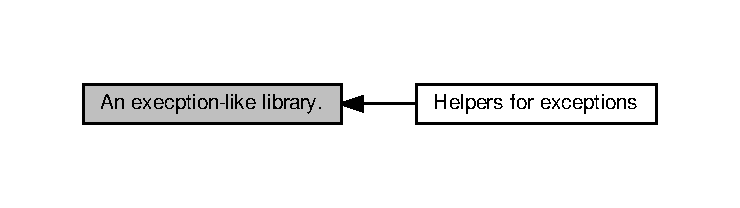
\includegraphics[width=350pt]{group__exceptions}
\end{center}
\end{figure}
\subsection*{Modules}
\begin{DoxyCompactItemize}
\item 
\hyperlink{group__helpers}{Helpers for exceptions}
\begin{DoxyCompactList}\small\item\em These are some internal helpers, not part of the public A\+PI. \end{DoxyCompactList}\end{DoxyCompactItemize}
\subsection*{Data Structures}
\begin{DoxyCompactItemize}
\item 
struct \hyperlink{structexception__handler__frame}{exception\+\_\+handler\+\_\+frame}
\item 
struct \hyperlink{structexception__stack__frame}{exception\+\_\+stack\+\_\+frame}
\end{DoxyCompactItemize}
\subsection*{Macros}
\begin{DoxyCompactItemize}
\item 
\#define {\bfseries \+\_\+\+\_\+concatenate\+\_\+tokens}(x,  y)~x \#\# y\hypertarget{group__exceptions_gadf8cc03bd0ede7f3e5aafa57de5016dd}{}\label{group__exceptions_gadf8cc03bd0ede7f3e5aafa57de5016dd}

\item 
\#define {\bfseries \+\_\+\+\_\+conc}(z,  w)~\+\_\+\+\_\+concatenate\+\_\+tokens(z,w)\hypertarget{group__exceptions_ga0d2e02c74b05d3ff3bfa9eb3dcd891e3}{}\label{group__exceptions_ga0d2e02c74b05d3ff3bfa9eb3dcd891e3}

\end{DoxyCompactItemize}
\subsection*{Typedefs}
\begin{DoxyCompactItemize}
\item 
typedef void($\ast$ {\bfseries exception\+\_\+handler}) (int)\hypertarget{group__exceptions_ga07c60bc46505779b049ce597fe609258}{}\label{group__exceptions_ga07c60bc46505779b049ce597fe609258}

\item 
typedef struct \hyperlink{structexception__stack__frame}{exception\+\_\+stack\+\_\+frame} $\ast$$\ast$ {\bfseries exception\+\_\+context}\hypertarget{group__exceptions_ga644495f4913e96a83cdf2779fd813974}{}\label{group__exceptions_ga644495f4913e96a83cdf2779fd813974}

\end{DoxyCompactItemize}
\subsection*{Functions}
\begin{DoxyCompactItemize}
\item 
void {\bfseries raise\+\_\+exception} (\hyperlink{structexception__stack__frame}{exception\+\_\+context} context)\hypertarget{group__exceptions_ga7eda2653ee54e0c95e9d51b8fd873298}{}\label{group__exceptions_ga7eda2653ee54e0c95e9d51b8fd873298}

\item 
void {\bfseries exception\+\_\+unwind} (\hyperlink{structexception__stack__frame}{exception\+\_\+context} context, int errcode)\hypertarget{group__exceptions_ga5232fee2c414c5ff1ff44dc28c83cf42}{}\label{group__exceptions_ga5232fee2c414c5ff1ff44dc28c83cf42}

\item 
static void {\bfseries \+\_\+\+\_\+exc\+\_\+push\+\_\+frame} (\hyperlink{structexception__stack__frame}{exception\+\_\+context} context, struct \hyperlink{structexception__stack__frame}{exception\+\_\+stack\+\_\+frame} $\ast$frame)\hypertarget{group__exceptions_gad0ebd2587ae85b044e1306a026246a27}{}\label{group__exceptions_gad0ebd2587ae85b044e1306a026246a27}

\item 
static struct \hyperlink{structexception__stack__frame}{exception\+\_\+stack\+\_\+frame} $\ast$ {\bfseries \+\_\+\+\_\+exc\+\_\+try} (\hyperlink{structexception__stack__frame}{exception\+\_\+context} context, int errcode)\hypertarget{group__exceptions_ga47cfe7a060b16ac1cd9a4432853205dc}{}\label{group__exceptions_ga47cfe7a060b16ac1cd9a4432853205dc}

\item 
static struct \hyperlink{structexception__stack__frame}{exception\+\_\+stack\+\_\+frame} $\ast$ {\bfseries \+\_\+\+\_\+exc\+\_\+exit\+\_\+try} (\hyperlink{structexception__stack__frame}{exception\+\_\+context} context)\hypertarget{group__exceptions_ga9d85149bdb927245ff694068119412df}{}\label{group__exceptions_ga9d85149bdb927245ff694068119412df}

\end{DoxyCompactItemize}


\subsection{Detailed Description}
An exception-\/like mechanism for C. 

Exceptions are supported by many object-\/oriented languages, such as Java, C++ and Python, but not by C. This makes programming certain kinds of tasks somewhat complicated. These are tasks that can cause a thread to exit back through several layers of calls. For example, a system call may lead to a stack of nested calls to execute the code of a driver. If processing is to be rolled back to the point of entry to the kernel, all calls in that stack need to propagate the error. This makes coding tedious and error-\/prone.

In C, there is a standard-\/library facility that can be used to implement such functionality, available by including {\ttfamily $<$setjmp.\+h$>$}. The help is in the form of functions {\ttfamily setjmp()} and {\ttfamily longjmp} (and their vatiatons). In this library, these standard calls, wrapped by some suitable macros, and using some G\+NU G\+CC extensions (nested functions), provide some easy-\/to-\/use exception-\/like programming structures.

\subsubsection*{Examples}

Before we describe the details, we show some examples of the library\textquotesingle{}s use.

A try-\/block is declared as follows\+: 
\begin{DoxyCode}
TRY\_WITH(context) \{

    ON\_ERROR \{
        printf(\textcolor{stringliteral}{"Error in what I was doing\(\backslash\)n"});
        \textcolor{comment}{// After this, execute the finally }
    \}

    FINALLY(e) \{
        \textcolor{keywordflow}{if}(e) 
            printf(\textcolor{stringliteral}{"Continuing after error\(\backslash\)n"});         
        \textcolor{keywordflow}{else}
            printf(\textcolor{stringliteral}{"Finished without error\(\backslash\)n"});
    \}

    \textcolor{comment}{// do something here }
    \textcolor{keywordflow}{if}(error\_happens)
        raise\_exception(context);

    \textcolor{comment}{// or call a function that may call raise\_exception()}
    do\_something\_else();

    \textcolor{comment}{// If we leave here, FINALLY will be executed }
\}
\end{DoxyCode}


For example, one could do the following, to construct a composite resource\+: 
\begin{DoxyCode}
Resource r1, r2, r3;
TRY\_WITH(context) \{
    lock\_monitor();
    FINALLY(e) \{
        unlock\_monitor();
    \}

    \textcolor{comment}{// This may raise\_exception(...)}
    r1 = acquire\_resource1();
    ON\_ERROR \{
        release\_resource1(r1);
    \}

    \textcolor{comment}{// This may raise\_exception(...)}
    r2 = acquire\_resource2(r2);

    ON\_ERROR \{
        release\_resource2(r2);
    \}
    
    \textcolor{comment}{// This may raise\_exception(...)}
    r3 = acquire\_resrouce3(r1, r2);
\}
\textcolor{keywordflow}{return} r3;
\end{DoxyCode}


\subsubsection*{How it works}

The workings are based on the idea of an {\bfseries exception stack}. The elements of this stack are called {\bfseries exception stack frames} (E\+S\+Fs). Each thread should have its own exception stack. When a T\+R\+Y\+\_\+\+W\+I\+TH(...) block begins, a new E\+SF is pushed to the stack, and the block starts to execute.

Each E\+SF has two lists of functions of type @ exception\+\_\+handler, which is defined as {\ttfamily void ($\ast$)(int)}. The nodes for these lists are {\ttfamily struct \hyperlink{structexception__handler__frame}{exception\+\_\+handler\+\_\+frame}} objects. Initially, the new E\+SF has empty lists. The first list is the list of {\bfseries catchers} and the second is the list of {\bfseries finalizers}.

As the T\+R\+Y-\/block executes, execution reaches {\ttfamily F\+I\+N\+A\+L\+L\+Y()} and {\ttfamily O\+N\+\_\+\+E\+R\+R\+OR} blocks. When a {\ttfamily F\+I\+N\+A\+L\+L\+Y()} block is reached, a new handler is added to the finalizers list. When a {\ttfamily O\+N\+\_\+\+E\+R\+R\+OR} block is reached, a new handler is added to the catchers list.

If execution arrives at the end of the T\+R\+Y-\/block, the list of catchers is thrown away and the finalizers are executed (in reverse order, that is, last-\/in-\/first-\/out).

If at some point the function {\ttfamily raise\+\_\+exception()} is called, execution jumps back at the T\+R\+Y-\/block at the top of the exception stack. There, each catcher is first executed, followed by all the finalizers. At the end, the E\+SF is popped from the exception stack. Then, if at least one catcher did execute, the exception is considered handled, and execution continues after the T\+R\+Y-\/block. If however there was no catcher executed, and the exception stack is non-\/empty, then {\ttfamily raise\+\_\+exception()} is called again, to repeat the process.

An exception stack is defined simply as a pointer to {\ttfamily struct \hyperlink{structexception__stack__frame}{exception\+\_\+stack\+\_\+frame}}. An \+\_\+\+\_\+exception context\+\_\+\+\_\+is a pointer to such a pointer, that is, 
\begin{DoxyCode}
\textcolor{keyword}{typedef} \textcolor{keyword}{struct }\hyperlink{structexception__stack__frame}{exception\_stack\_frame}** exception\_context;
\end{DoxyCode}
 A context needs to be available to our code in two places\+: when a {\ttfamily T\+R\+Y\+\_\+\+W\+I\+T\+H(context)} block is defined, and when {\ttfamily raise\+\_\+exception(context)} is called.

One can simply define a context as a global variable\+: 
\begin{DoxyCode}
\textcolor{comment}{// at top level}
\textcolor{keyword}{struct }execution\_stack\_frame* exception\_stack = NULL;
\textcolor{preprocessor}{#define TRY  TRY\_WITH(&exception\_stack)}
\textcolor{preprocessor}{#define RAISE  raise\_exception(&exception\_stack)}

TRY \{
    ...
    RAISE;
    ...
\}
\end{DoxyCode}


In a multi-\/threaded case, it is necessary to declare one context for each thread. This can be done at the T\+CB, for example.


\begin{DoxyCode}
\textcolor{keyword}{struct }\hyperlink{structthread__control__block}{TCB} \{
    ....
    \textcolor{keyword}{struct }execution\_stack\_frame* exception\_stack = NULL;   
\}

\textcolor{preprocessor}{#define TRY  TRY\_WITH(& CURTHREAD->exception\_stack)}
\textcolor{preprocessor}{#define RAISE  raise\_exception(& CURTHREAD->exception\_stack)}
\end{DoxyCode}


\subsubsection*{Performance}

Although setting up a T\+R\+Y-\/block is relatively cheap (basically, a call to {\ttfamily setjmp} is done), it is better to avoid calling exception handlers. So, for very critical pieces of code, one could do 
\begin{DoxyCode}
TRY \{
    lock\_mutex();
    ON\_ERROR \{
        unlock\_mutex();
    \}

    ... \textcolor{comment}{// stuff}

    unlock\_mutex();
\}
\end{DoxyCode}
 instead of the more convenient 
\begin{DoxyCode}
TRY \{
    lock\_mutex();
    FINALLY(e) \{
        unlock\_mutex();
    \}

    ... \textcolor{comment}{// stuff    }
\}
\end{DoxyCode}


The first case is faster, because it avoids a function call, when there is no exception, whereas the second will make a call to the {\ttfamily F\+I\+N\+A\+L\+LY} block, even without an exception raised. But, remember\+: {\bfseries premature optimization is the source of all evil}.

\subsubsection*{Raising from inside an exception handler}

It is perfecly legal and supported to have exceptions raised from inside {\ttfamily O\+N\+\_\+\+E\+R\+R\+OR} or {\ttfamily F\+I\+N\+A\+L\+LY} blocks (or the functions they call).

What happens in this case is that the exception handler execution is aborted and the processing continues with the next exception handler of the E\+SF. 
\hypertarget{group__helpers}{}\section{Helpers for exceptions}
\label{group__helpers}\index{Helpers for exceptions@{Helpers for exceptions}}


These are some internal helpers, not part of the public A\+PI.  


Collaboration diagram for Helpers for exceptions\+:\nopagebreak
\begin{figure}[H]
\begin{center}
\leavevmode
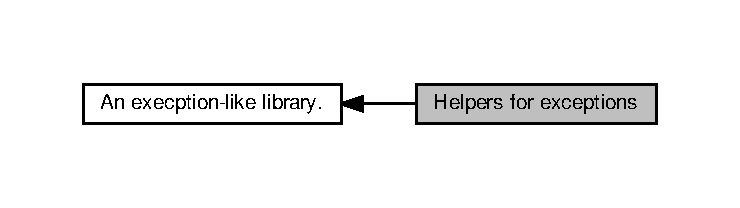
\includegraphics[width=350pt]{group__helpers}
\end{center}
\end{figure}
These are some internal helpers, not part of the public A\+PI. 


\chapter{Data Structure Documentation}
\hypertarget{struct____rs__globals}{}\section{\+\_\+\+\_\+rs\+\_\+globals Struct Reference}
\label{struct____rs__globals}\index{\+\_\+\+\_\+rs\+\_\+globals@{\+\_\+\+\_\+rs\+\_\+globals}}


Collaboration diagram for \+\_\+\+\_\+rs\+\_\+globals\+:
\nopagebreak
\begin{figure}[H]
\begin{center}
\leavevmode
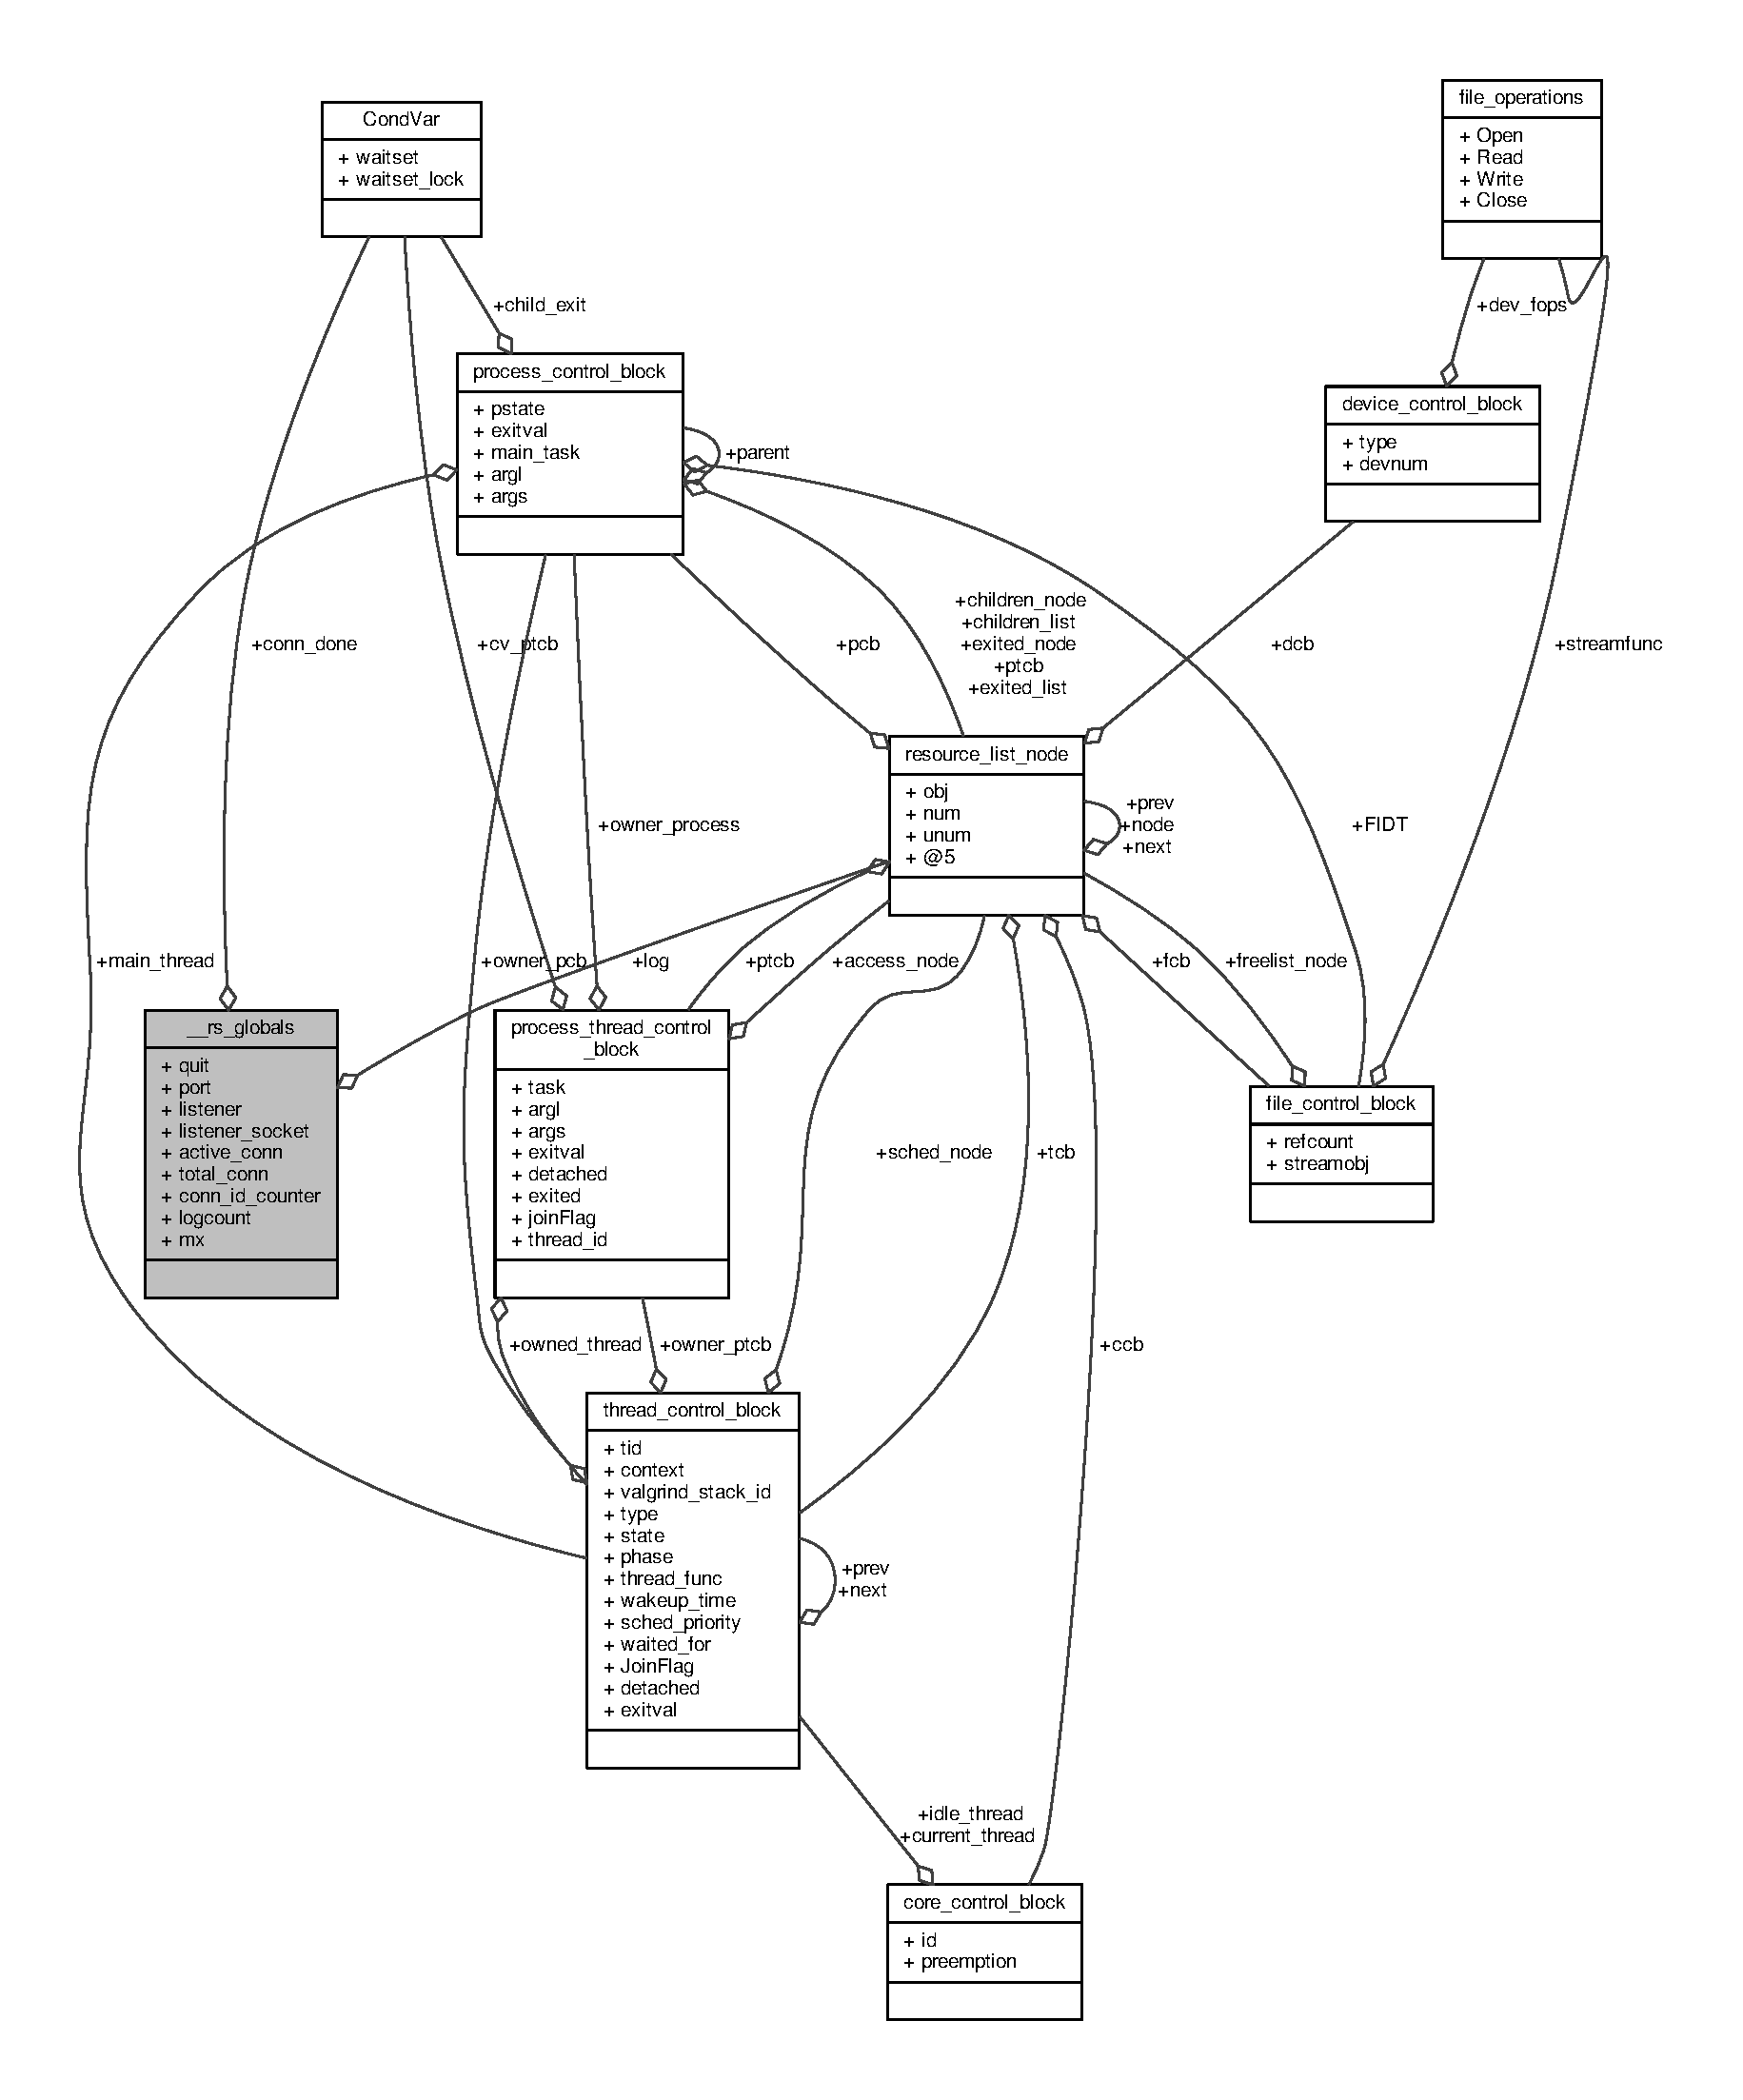
\includegraphics[width=350pt]{struct____rs__globals__coll__graph}
\end{center}
\end{figure}
\subsection*{Data Fields}
\begin{DoxyCompactItemize}
\item 
int {\bfseries quit}\hypertarget{struct____rs__globals_a883fedeeb83e8f30d55072af301365a4}{}\label{struct____rs__globals_a883fedeeb83e8f30d55072af301365a4}

\item 
\hyperlink{group__syscalls_ga13894e5a2ffd5febb7aeb90e87239d61}{port\+\_\+t} {\bfseries port}\hypertarget{struct____rs__globals_a6dc49afd76e2743a62e0a467ab5af41b}{}\label{struct____rs__globals_a6dc49afd76e2743a62e0a467ab5af41b}

\item 
\hyperlink{group__syscalls_gaf67ad1c55e6b2a79bf8a99106380ce01}{Tid\+\_\+t} {\bfseries listener}\hypertarget{struct____rs__globals_afc8fa99b7b3fcee63f780cc0e3690ebf}{}\label{struct____rs__globals_afc8fa99b7b3fcee63f780cc0e3690ebf}

\item 
\hyperlink{group__syscalls_ga5097222c5f0da97d92d4712359abc38f}{Fid\+\_\+t} {\bfseries listener\+\_\+socket}\hypertarget{struct____rs__globals_a7f274f9a80478d9b33b743e1432f2438}{}\label{struct____rs__globals_a7f274f9a80478d9b33b743e1432f2438}

\item 
size\+\_\+t {\bfseries active\+\_\+conn}\hypertarget{struct____rs__globals_ad1be788d826e6e30ab8df0f12d6a53a3}{}\label{struct____rs__globals_ad1be788d826e6e30ab8df0f12d6a53a3}

\item 
size\+\_\+t {\bfseries total\+\_\+conn}\hypertarget{struct____rs__globals_ad4f03cddafaa93561024a6ab26c937d3}{}\label{struct____rs__globals_ad4f03cddafaa93561024a6ab26c937d3}

\item 
size\+\_\+t {\bfseries conn\+\_\+id\+\_\+counter}\hypertarget{struct____rs__globals_a914de4c47a4da5f5df4fa5c4a1de899b}{}\label{struct____rs__globals_a914de4c47a4da5f5df4fa5c4a1de899b}

\item 
\hyperlink{group__rlists_ga8f6244877f7ce2322c90525217ea6e7a}{rlnode} {\bfseries log}\hypertarget{struct____rs__globals_a8578087e09ae301d77b81dd2b5a661fa}{}\label{struct____rs__globals_a8578087e09ae301d77b81dd2b5a661fa}

\item 
size\+\_\+t {\bfseries logcount}\hypertarget{struct____rs__globals_ad1001e26c768cecab1408d19f025d3f8}{}\label{struct____rs__globals_ad1001e26c768cecab1408d19f025d3f8}

\item 
\hyperlink{group__syscalls_gaef2ec62cae8e0031fd19fc8b91083ade}{Mutex} {\bfseries mx}\hypertarget{struct____rs__globals_ae6f58855b0c5911cacb493a1f305c9e3}{}\label{struct____rs__globals_ae6f58855b0c5911cacb493a1f305c9e3}

\item 
\hyperlink{structCondVar}{Cond\+Var} {\bfseries conn\+\_\+done}\hypertarget{struct____rs__globals_acded897204308c539cab184093cd6207}{}\label{struct____rs__globals_acded897204308c539cab184093cd6207}

\end{DoxyCompactItemize}


\subsection{Detailed Description}


Definition at line 407 of file tinyos\+\_\+shell.\+c.



The documentation for this struct was generated from the following file\+:\begin{DoxyCompactItemize}
\item 
tinyos\+\_\+shell.\+c\end{DoxyCompactItemize}

\hypertarget{structCondVar}{}\section{Cond\+Var Struct Reference}
\label{structCondVar}\index{Cond\+Var@{Cond\+Var}}


Condition variables.  




{\ttfamily \#include $<$tinyos.\+h$>$}



Collaboration diagram for Cond\+Var\+:\nopagebreak
\begin{figure}[H]
\begin{center}
\leavevmode
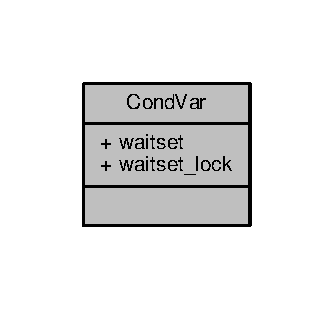
\includegraphics[width=160pt]{structCondVar__coll__graph}
\end{center}
\end{figure}
\subsection*{Data Fields}
\begin{DoxyCompactItemize}
\item 
void $\ast$ \hyperlink{structCondVar_a7da9e0169713c3b3ae386a8ab49f7e34}{waitset}
\item 
\hyperlink{group__syscalls_gaef2ec62cae8e0031fd19fc8b91083ade}{Mutex} \hyperlink{structCondVar_a477b855f4d3880d231206ae79bd5b6cf}{waitset\+\_\+lock}
\end{DoxyCompactItemize}


\subsection{Detailed Description}
Condition variables. 

A condition variable is used for longer synchronization. This implementation can be used both in the pre-\/emptive and in the non-\/preemptive domain.

\begin{DoxySeeAlso}{See also}
\hyperlink{group__syscalls_ga970dca2210b3f2ec8aedab7f542a9bf4}{Cond\+\_\+\+Wait} 

\hyperlink{group__syscalls_ga43f64f8be273d2fe77d7de5f4b81e22d}{Cond\+\_\+\+Signal} 

\hyperlink{group__syscalls_ga8196aa2a48cad90742f254cc3b8fd351}{Cond\+\_\+\+Broadcast} 

\hyperlink{group__syscalls_ga6a7055a466bff255172e05f6ec82d792}{C\+O\+N\+D\+\_\+\+I\+N\+IT} 
\end{DoxySeeAlso}


Definition at line 123 of file tinyos.\+h.



\subsection{Field Documentation}
\index{Cond\+Var@{Cond\+Var}!waitset@{waitset}}
\index{waitset@{waitset}!Cond\+Var@{Cond\+Var}}
\subsubsection[{\texorpdfstring{waitset}{waitset}}]{\setlength{\rightskip}{0pt plus 5cm}void$\ast$ Cond\+Var\+::waitset}\hypertarget{structCondVar_a7da9e0169713c3b3ae386a8ab49f7e34}{}\label{structCondVar_a7da9e0169713c3b3ae386a8ab49f7e34}
The set of waiting threads 

Definition at line 124 of file tinyos.\+h.

\index{Cond\+Var@{Cond\+Var}!waitset\+\_\+lock@{waitset\+\_\+lock}}
\index{waitset\+\_\+lock@{waitset\+\_\+lock}!Cond\+Var@{Cond\+Var}}
\subsubsection[{\texorpdfstring{waitset\+\_\+lock}{waitset_lock}}]{\setlength{\rightskip}{0pt plus 5cm}{\bf Mutex} Cond\+Var\+::waitset\+\_\+lock}\hypertarget{structCondVar_a477b855f4d3880d231206ae79bd5b6cf}{}\label{structCondVar_a477b855f4d3880d231206ae79bd5b6cf}
A mutex to protect {\ttfamily waitset} 

Definition at line 125 of file tinyos.\+h.



The documentation for this struct was generated from the following file\+:\begin{DoxyCompactItemize}
\item 
\hyperlink{tinyos_8h}{tinyos.\+h}\end{DoxyCompactItemize}

\hypertarget{structcore__control__block}{}\section{core\+\_\+control\+\_\+block Struct Reference}
\label{structcore__control__block}\index{core\+\_\+control\+\_\+block@{core\+\_\+control\+\_\+block}}


Core control block.  




{\ttfamily \#include $<$kernel\+\_\+sched.\+h$>$}



Collaboration diagram for core\+\_\+control\+\_\+block\+:
\nopagebreak
\begin{figure}[H]
\begin{center}
\leavevmode
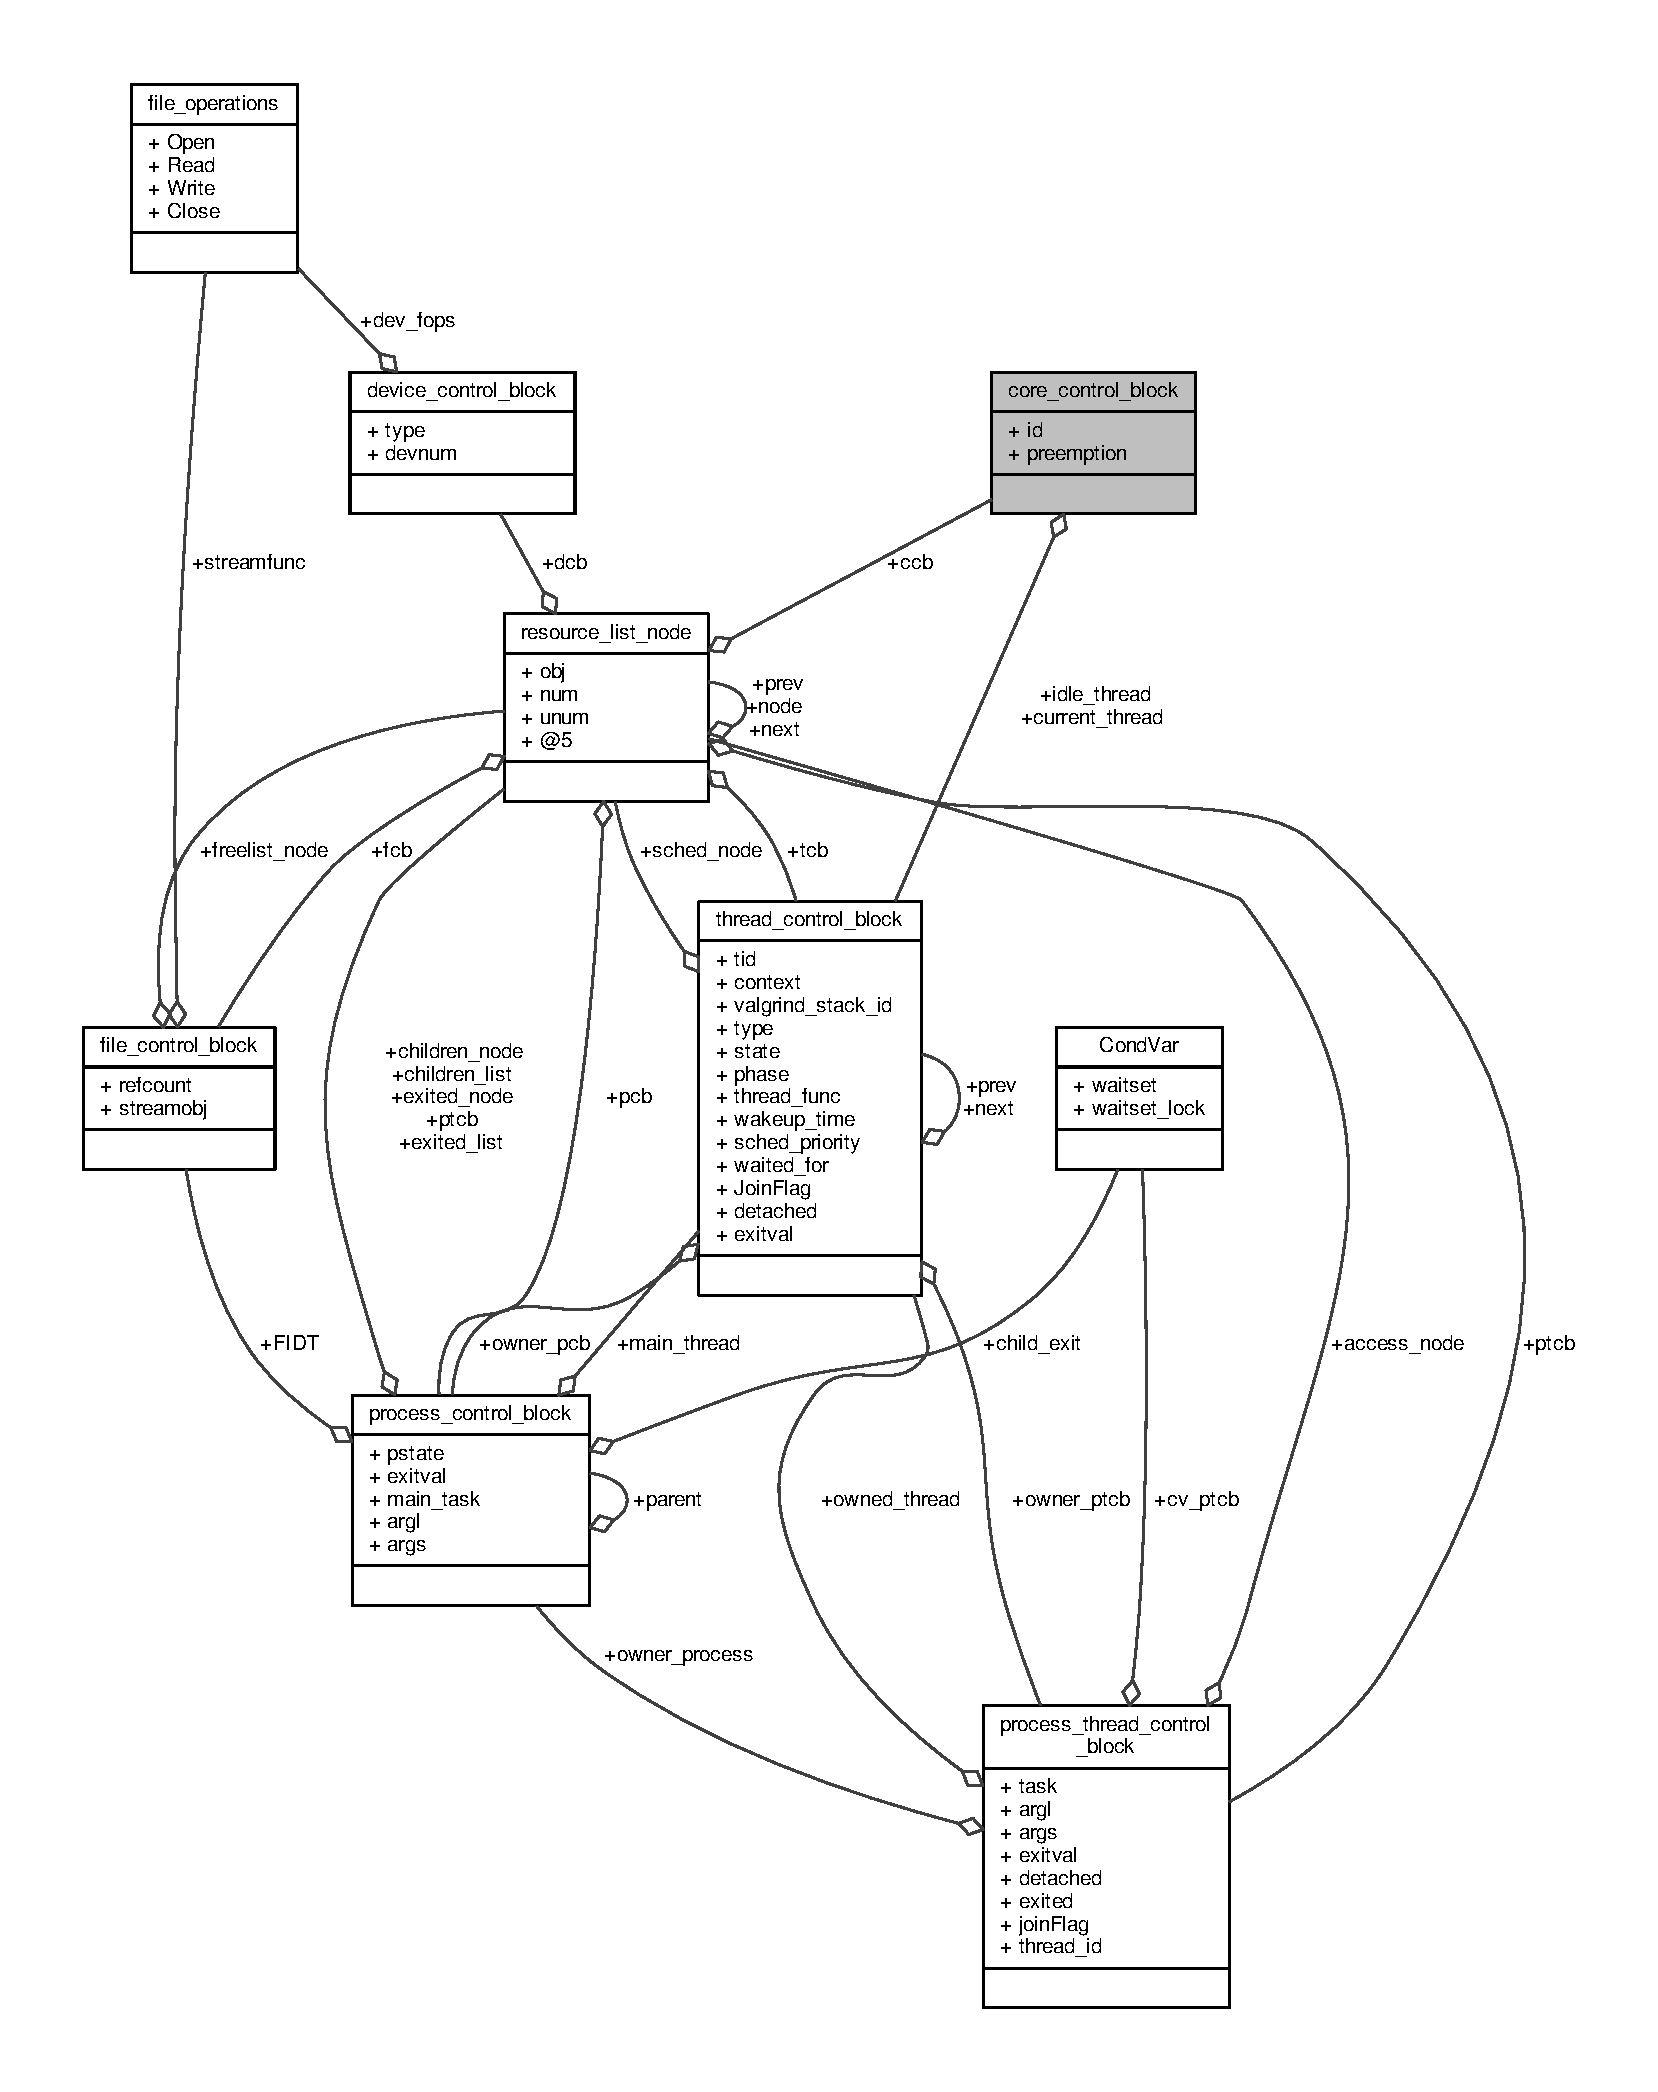
\includegraphics[width=350pt]{structcore__control__block__coll__graph}
\end{center}
\end{figure}
\subsection*{Data Fields}
\begin{DoxyCompactItemize}
\item 
\hyperlink{bios_8h_a91ad9478d81a7aaf2593e8d9c3d06a14}{uint} \hyperlink{structcore__control__block_a5208867f309bdd1656fd473f38b30bfe}{id}
\item 
\hyperlink{group__scheduler_gaf88d9c946bf70b36a1e8bc34383abfc9}{T\+CB} $\ast$ \hyperlink{structcore__control__block_aac649db5b9a99e693ed21c7e610834bf}{current\+\_\+thread}
\item 
\hyperlink{group__scheduler_gaf88d9c946bf70b36a1e8bc34383abfc9}{T\+CB} \hyperlink{structcore__control__block_a6dd29dab4a95ce740f45370345408c52}{idle\+\_\+thread}
\item 
sig\+\_\+atomic\+\_\+t \hyperlink{structcore__control__block_a858cde45d4478d73f60e839594b363f4}{preemption}
\end{DoxyCompactItemize}


\subsection{Detailed Description}
Core control block. 

Per-\/core info in memory (basically scheduler-\/related) 

Definition at line 149 of file kernel\+\_\+sched.\+h.



\subsection{Field Documentation}
\index{core\+\_\+control\+\_\+block@{core\+\_\+control\+\_\+block}!current\+\_\+thread@{current\+\_\+thread}}
\index{current\+\_\+thread@{current\+\_\+thread}!core\+\_\+control\+\_\+block@{core\+\_\+control\+\_\+block}}
\subsubsection[{\texorpdfstring{current\+\_\+thread}{current_thread}}]{\setlength{\rightskip}{0pt plus 5cm}{\bf T\+CB}$\ast$ core\+\_\+control\+\_\+block\+::current\+\_\+thread}\hypertarget{structcore__control__block_aac649db5b9a99e693ed21c7e610834bf}{}\label{structcore__control__block_aac649db5b9a99e693ed21c7e610834bf}
Points to the thread currently owning the core 

Definition at line 152 of file kernel\+\_\+sched.\+h.

\index{core\+\_\+control\+\_\+block@{core\+\_\+control\+\_\+block}!id@{id}}
\index{id@{id}!core\+\_\+control\+\_\+block@{core\+\_\+control\+\_\+block}}
\subsubsection[{\texorpdfstring{id}{id}}]{\setlength{\rightskip}{0pt plus 5cm}{\bf uint} core\+\_\+control\+\_\+block\+::id}\hypertarget{structcore__control__block_a5208867f309bdd1656fd473f38b30bfe}{}\label{structcore__control__block_a5208867f309bdd1656fd473f38b30bfe}
The core id 

Definition at line 150 of file kernel\+\_\+sched.\+h.

\index{core\+\_\+control\+\_\+block@{core\+\_\+control\+\_\+block}!idle\+\_\+thread@{idle\+\_\+thread}}
\index{idle\+\_\+thread@{idle\+\_\+thread}!core\+\_\+control\+\_\+block@{core\+\_\+control\+\_\+block}}
\subsubsection[{\texorpdfstring{idle\+\_\+thread}{idle_thread}}]{\setlength{\rightskip}{0pt plus 5cm}{\bf T\+CB} core\+\_\+control\+\_\+block\+::idle\+\_\+thread}\hypertarget{structcore__control__block_a6dd29dab4a95ce740f45370345408c52}{}\label{structcore__control__block_a6dd29dab4a95ce740f45370345408c52}
Used by the scheduler to handle the core\textquotesingle{}s idle thread 

Definition at line 153 of file kernel\+\_\+sched.\+h.

\index{core\+\_\+control\+\_\+block@{core\+\_\+control\+\_\+block}!preemption@{preemption}}
\index{preemption@{preemption}!core\+\_\+control\+\_\+block@{core\+\_\+control\+\_\+block}}
\subsubsection[{\texorpdfstring{preemption}{preemption}}]{\setlength{\rightskip}{0pt plus 5cm}sig\+\_\+atomic\+\_\+t core\+\_\+control\+\_\+block\+::preemption}\hypertarget{structcore__control__block_a858cde45d4478d73f60e839594b363f4}{}\label{structcore__control__block_a858cde45d4478d73f60e839594b363f4}
Marks preemption, used by the locking code 

Definition at line 154 of file kernel\+\_\+sched.\+h.



The documentation for this struct was generated from the following file\+:\begin{DoxyCompactItemize}
\item 
\hyperlink{kernel__sched_8h}{kernel\+\_\+sched.\+h}\end{DoxyCompactItemize}

\hypertarget{structdevice__control__block}{}\section{device\+\_\+control\+\_\+block Struct Reference}
\label{structdevice__control__block}\index{device\+\_\+control\+\_\+block@{device\+\_\+control\+\_\+block}}


Device control block.  




{\ttfamily \#include $<$kernel\+\_\+dev.\+h$>$}



Collaboration diagram for device\+\_\+control\+\_\+block\+:\nopagebreak
\begin{figure}[H]
\begin{center}
\leavevmode
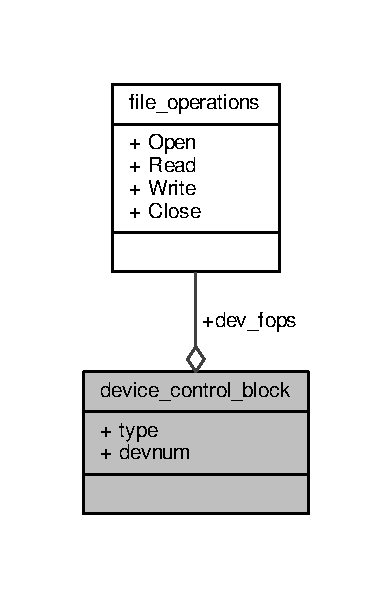
\includegraphics[width=188pt]{structdevice__control__block__coll__graph}
\end{center}
\end{figure}
\subsection*{Data Fields}
\begin{DoxyCompactItemize}
\item 
\hyperlink{group__dev_ga879ceac20e83b2375e5b49f4379b0c90}{Device\+\_\+type} \hyperlink{structdevice__control__block_a35a45268132777177a33513c747633c4}{type}\hypertarget{structdevice__control__block_a35a45268132777177a33513c747633c4}{}\label{structdevice__control__block_a35a45268132777177a33513c747633c4}

\begin{DoxyCompactList}\small\item\em Device type. Much like \textquotesingle{}major number\textquotesingle{} in Unix, determines the driver. \end{DoxyCompactList}\item 
\hyperlink{bios_8h_a91ad9478d81a7aaf2593e8d9c3d06a14}{uint} \hyperlink{structdevice__control__block_a25d8f038a1c6d41f445d078276117fba}{devnum}\hypertarget{structdevice__control__block_a25d8f038a1c6d41f445d078276117fba}{}\label{structdevice__control__block_a25d8f038a1c6d41f445d078276117fba}

\begin{DoxyCompactList}\small\item\em Number of devices for this major number. \end{DoxyCompactList}\item 
\hyperlink{group__dev_gaab625d8ae3a95e942ed10ed1579f5042}{file\+\_\+ops} \hyperlink{structdevice__control__block_a2945d5da96f40ff7fae94e295624a7c7}{dev\+\_\+fops}\hypertarget{structdevice__control__block_a2945d5da96f40ff7fae94e295624a7c7}{}\label{structdevice__control__block_a2945d5da96f40ff7fae94e295624a7c7}

\begin{DoxyCompactList}\small\item\em Device operations This structure is provided by the device driver. \end{DoxyCompactList}\end{DoxyCompactItemize}


\subsection{Detailed Description}
Device control block. 

These objects hold the information that is needed to access a particular device. 

Definition at line 117 of file kernel\+\_\+dev.\+h.



The documentation for this struct was generated from the following file\+:\begin{DoxyCompactItemize}
\item 
\hyperlink{kernel__dev_8h}{kernel\+\_\+dev.\+h}\end{DoxyCompactItemize}

\hypertarget{structexception__handler__frame}{}\section{exception\+\_\+handler\+\_\+frame Struct Reference}
\label{structexception__handler__frame}\index{exception\+\_\+handler\+\_\+frame@{exception\+\_\+handler\+\_\+frame}}


Collaboration diagram for exception\+\_\+handler\+\_\+frame\+:\nopagebreak
\begin{figure}[H]
\begin{center}
\leavevmode
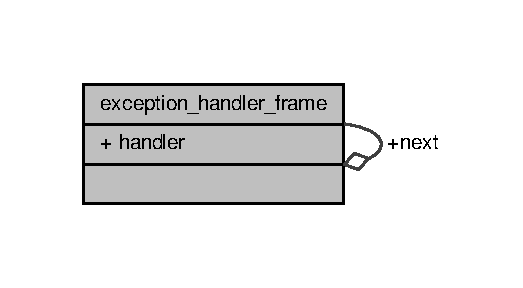
\includegraphics[width=251pt]{structexception__handler__frame__coll__graph}
\end{center}
\end{figure}
\subsection*{Data Fields}
\begin{DoxyCompactItemize}
\item 
exception\+\_\+handler {\bfseries handler}\hypertarget{structexception__handler__frame_a9df815cc8cec8aace242043b89fb44e8}{}\label{structexception__handler__frame_a9df815cc8cec8aace242043b89fb44e8}

\item 
struct \hyperlink{structexception__handler__frame}{exception\+\_\+handler\+\_\+frame} $\ast$ {\bfseries next}\hypertarget{structexception__handler__frame_a407cf31d00d01b49b1774dea464c29cf}{}\label{structexception__handler__frame_a407cf31d00d01b49b1774dea464c29cf}

\end{DoxyCompactItemize}


\subsection{Detailed Description}


Definition at line 870 of file util.\+h.



The documentation for this struct was generated from the following file\+:\begin{DoxyCompactItemize}
\item 
\hyperlink{util_8h}{util.\+h}\end{DoxyCompactItemize}

\hypertarget{structexception__stack__frame}{}\section{exception\+\_\+stack\+\_\+frame Struct Reference}
\label{structexception__stack__frame}\index{exception\+\_\+stack\+\_\+frame@{exception\+\_\+stack\+\_\+frame}}


Collaboration diagram for exception\+\_\+stack\+\_\+frame\+:\nopagebreak
\begin{figure}[H]
\begin{center}
\leavevmode
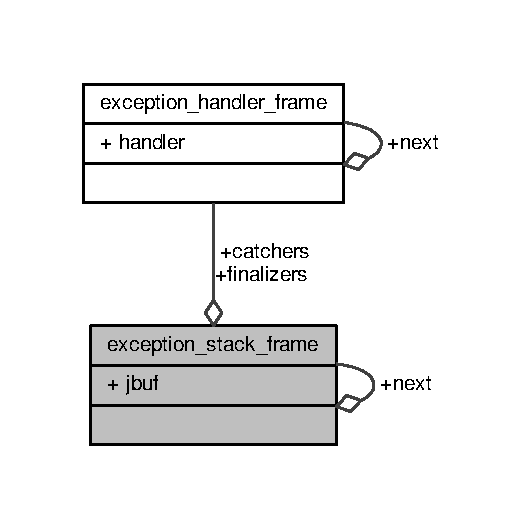
\includegraphics[width=251pt]{structexception__stack__frame__coll__graph}
\end{center}
\end{figure}
\subsection*{Data Fields}
\begin{DoxyCompactItemize}
\item 
struct \hyperlink{structexception__stack__frame}{exception\+\_\+stack\+\_\+frame} $\ast$ {\bfseries next}\hypertarget{structexception__stack__frame_abb538d9a6f6155ed83f140dd2adb7457}{}\label{structexception__stack__frame_abb538d9a6f6155ed83f140dd2adb7457}

\item 
struct \hyperlink{structexception__handler__frame}{exception\+\_\+handler\+\_\+frame} $\ast$ {\bfseries catchers}\hypertarget{structexception__stack__frame_a950ab78cc930f9662ff9cb7eedcfda79}{}\label{structexception__stack__frame_a950ab78cc930f9662ff9cb7eedcfda79}

\item 
struct \hyperlink{structexception__handler__frame}{exception\+\_\+handler\+\_\+frame} $\ast$ {\bfseries finalizers}\hypertarget{structexception__stack__frame_a543e62e78b4b2777e9df32ccc5feba38}{}\label{structexception__stack__frame_a543e62e78b4b2777e9df32ccc5feba38}

\item 
jmp\+\_\+buf {\bfseries jbuf}\hypertarget{structexception__stack__frame_a6f81386a697bcae78000625ee8ba02fa}{}\label{structexception__stack__frame_a6f81386a697bcae78000625ee8ba02fa}

\end{DoxyCompactItemize}


\subsection{Detailed Description}


Definition at line 876 of file util.\+h.



The documentation for this struct was generated from the following file\+:\begin{DoxyCompactItemize}
\item 
\hyperlink{util_8h}{util.\+h}\end{DoxyCompactItemize}

\hypertarget{structfile__control__block}{}\section{file\+\_\+control\+\_\+block Struct Reference}
\label{structfile__control__block}\index{file\+\_\+control\+\_\+block@{file\+\_\+control\+\_\+block}}


The file control block.  




{\ttfamily \#include $<$kernel\+\_\+streams.\+h$>$}



Collaboration diagram for file\+\_\+control\+\_\+block\+:
\nopagebreak
\begin{figure}[H]
\begin{center}
\leavevmode
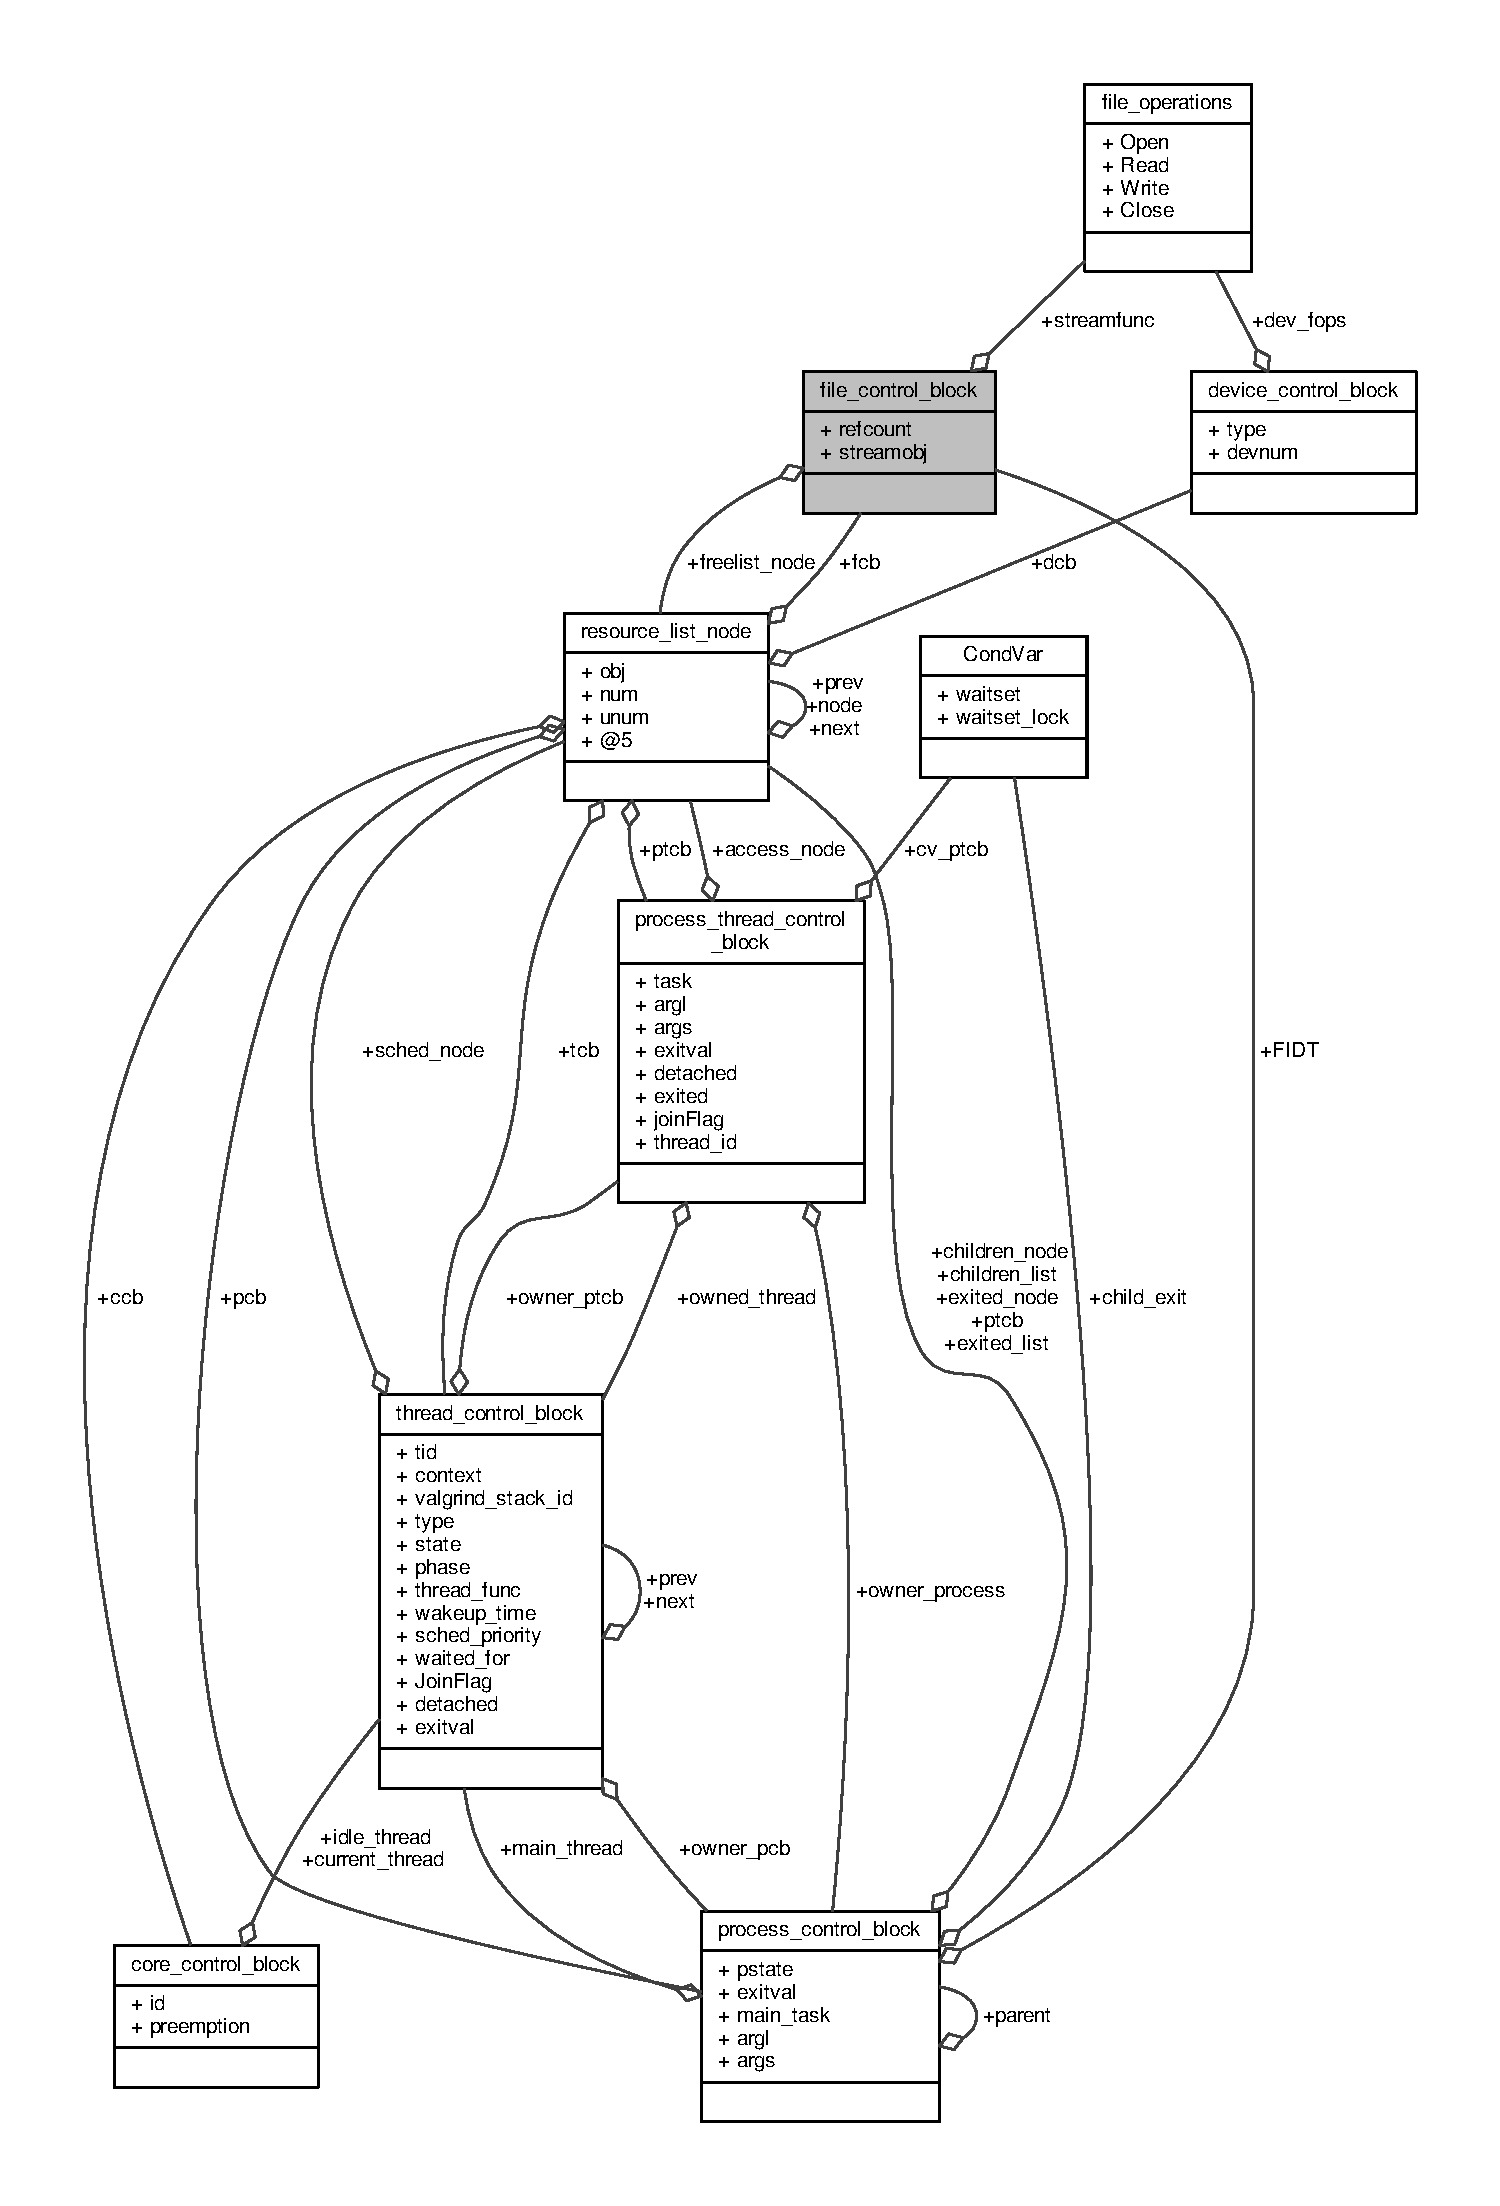
\includegraphics[width=350pt]{structfile__control__block__coll__graph}
\end{center}
\end{figure}
\subsection*{Data Fields}
\begin{DoxyCompactItemize}
\item 
\hyperlink{bios_8h_a91ad9478d81a7aaf2593e8d9c3d06a14}{uint} \hyperlink{structfile__control__block_a629271d79f15500a74096ec65a4adedb}{refcount}\hypertarget{structfile__control__block_a629271d79f15500a74096ec65a4adedb}{}\label{structfile__control__block_a629271d79f15500a74096ec65a4adedb}

\begin{DoxyCompactList}\small\item\em Reference counter. \end{DoxyCompactList}\item 
void $\ast$ \hyperlink{structfile__control__block_a1460eb54b4a65e747b9b9ec3f6a798d6}{streamobj}\hypertarget{structfile__control__block_a1460eb54b4a65e747b9b9ec3f6a798d6}{}\label{structfile__control__block_a1460eb54b4a65e747b9b9ec3f6a798d6}

\begin{DoxyCompactList}\small\item\em The stream object (e.\+g., a device) \end{DoxyCompactList}\item 
\hyperlink{group__dev_gaab625d8ae3a95e942ed10ed1579f5042}{file\+\_\+ops} $\ast$ \hyperlink{structfile__control__block_aa49f26d3baceeb074fa00f9e5caf978b}{streamfunc}\hypertarget{structfile__control__block_aa49f26d3baceeb074fa00f9e5caf978b}{}\label{structfile__control__block_aa49f26d3baceeb074fa00f9e5caf978b}

\begin{DoxyCompactList}\small\item\em The stream implementation methods. \end{DoxyCompactList}\item 
\hyperlink{group__rlists_ga8f6244877f7ce2322c90525217ea6e7a}{rlnode} \hyperlink{structfile__control__block_ac84640123f400fa3fe3cb64df08e6bd6}{freelist\+\_\+node}\hypertarget{structfile__control__block_ac84640123f400fa3fe3cb64df08e6bd6}{}\label{structfile__control__block_ac84640123f400fa3fe3cb64df08e6bd6}

\begin{DoxyCompactList}\small\item\em Intrusive list node. \end{DoxyCompactList}\end{DoxyCompactItemize}


\subsection{Detailed Description}
The file control block. 

A file control block provides a uniform object to the system calls, and contains pointers to device-\/specific functions. 

Definition at line 41 of file kernel\+\_\+streams.\+h.



The documentation for this struct was generated from the following file\+:\begin{DoxyCompactItemize}
\item 
\hyperlink{kernel__streams_8h}{kernel\+\_\+streams.\+h}\end{DoxyCompactItemize}

\hypertarget{structfile__operations}{}\section{file\+\_\+operations Struct Reference}
\label{structfile__operations}\index{file\+\_\+operations@{file\+\_\+operations}}


The device-\/specific file operations table.  




{\ttfamily \#include $<$kernel\+\_\+dev.\+h$>$}



Collaboration diagram for file\+\_\+operations\+:\nopagebreak
\begin{figure}[H]
\begin{center}
\leavevmode
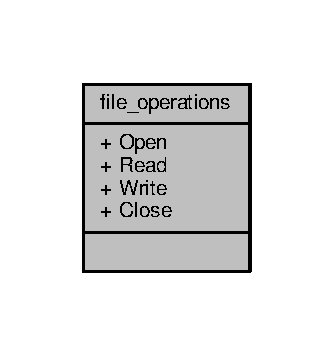
\includegraphics[width=160pt]{structfile__operations__coll__graph}
\end{center}
\end{figure}
\subsection*{Data Fields}
\begin{DoxyCompactItemize}
\item 
void $\ast$($\ast$ \hyperlink{structfile__operations_a2732da2af03e1fc7ba0b63a529ab1411}{Open} )(\hyperlink{bios_8h_a91ad9478d81a7aaf2593e8d9c3d06a14}{uint} minor)
\begin{DoxyCompactList}\small\item\em Return a stream object on which the other methods will operate. \end{DoxyCompactList}\item 
int($\ast$ \hyperlink{structfile__operations_a59d973a490a6861c498ac9cc9c32dbf5}{Read} )(void $\ast$this, char $\ast$buf, unsigned int size)
\begin{DoxyCompactList}\small\item\em Read operation. \end{DoxyCompactList}\item 
int($\ast$ \hyperlink{structfile__operations_a75d4020e8a146c1611dc40184d211ec6}{Write} )(void $\ast$this, const char $\ast$buf, unsigned int size)
\begin{DoxyCompactList}\small\item\em Write operation. \end{DoxyCompactList}\item 
int($\ast$ \hyperlink{structfile__operations_a66cfe706a1a29e3e58c7694dbd801b0f}{Close} )(void $\ast$this)
\begin{DoxyCompactList}\small\item\em Close operation. \end{DoxyCompactList}\end{DoxyCompactItemize}


\subsection{Detailed Description}
The device-\/specific file operations table. 

This object contains pointers to device-\/specific functions for I/O. Device drivers and other resource managers which expose a stream interface, must implement these methods.

The first argument of each method is taken from the \textquotesingle{}streamobj\textquotesingle{} field of the F\+CB. \begin{DoxySeeAlso}{See also}
\hyperlink{group__rlists_ga60c6c294fa1d8ea73ed270404fe5c17d}{F\+CB} 
\end{DoxySeeAlso}


Definition at line 48 of file kernel\+\_\+dev.\+h.



\subsection{Field Documentation}
\index{file\+\_\+operations@{file\+\_\+operations}!Close@{Close}}
\index{Close@{Close}!file\+\_\+operations@{file\+\_\+operations}}
\subsubsection[{\texorpdfstring{Close}{Close}}]{\setlength{\rightskip}{0pt plus 5cm}int($\ast$ file\+\_\+operations\+::\+Close) (void $\ast$this)}\hypertarget{structfile__operations_a66cfe706a1a29e3e58c7694dbd801b0f}{}\label{structfile__operations_a66cfe706a1a29e3e58c7694dbd801b0f}


Close operation. 

Close the stream object, deallocating any resources held by it. This function returns 0 is it was successful and -\/1 if not. Although the value in case of failure is passed to the calling process, the stream should still be destroyed.

Possible errors are\+:
\begin{DoxyItemize}
\item There was a I/O runtime problem. 
\end{DoxyItemize}

Definition at line 94 of file kernel\+\_\+dev.\+h.

\index{file\+\_\+operations@{file\+\_\+operations}!Open@{Open}}
\index{Open@{Open}!file\+\_\+operations@{file\+\_\+operations}}
\subsubsection[{\texorpdfstring{Open}{Open}}]{\setlength{\rightskip}{0pt plus 5cm}void$\ast$($\ast$ file\+\_\+operations\+::\+Open) ({\bf uint} minor)}\hypertarget{structfile__operations_a2732da2af03e1fc7ba0b63a529ab1411}{}\label{structfile__operations_a2732da2af03e1fc7ba0b63a529ab1411}


Return a stream object on which the other methods will operate. 

This function is passed the minor number of the device to be accessed. 

Definition at line 55 of file kernel\+\_\+dev.\+h.

\index{file\+\_\+operations@{file\+\_\+operations}!Read@{Read}}
\index{Read@{Read}!file\+\_\+operations@{file\+\_\+operations}}
\subsubsection[{\texorpdfstring{Read}{Read}}]{\setlength{\rightskip}{0pt plus 5cm}int($\ast$ file\+\_\+operations\+::\+Read) (void $\ast$this, char $\ast$buf, unsigned int size)}\hypertarget{structfile__operations_a59d973a490a6861c498ac9cc9c32dbf5}{}\label{structfile__operations_a59d973a490a6861c498ac9cc9c32dbf5}


Read operation. 

Read up to \textquotesingle{}size\textquotesingle{} bytes from stream \textquotesingle{}this\textquotesingle{} into buffer \textquotesingle{}buf\textquotesingle{}. If no data is available, the thread will block, to wait for data. The Read function should return the number of bytes copied into buf, or -\/1 on error. The call may return fewer bytes than \textquotesingle{}size\textquotesingle{}, but at least 1. A value of 0 indicates \char`\"{}end of data\char`\"{}.

Possible errors are\+:
\begin{DoxyItemize}
\item There was a I/O runtime problem. 
\end{DoxyItemize}

Definition at line 69 of file kernel\+\_\+dev.\+h.

\index{file\+\_\+operations@{file\+\_\+operations}!Write@{Write}}
\index{Write@{Write}!file\+\_\+operations@{file\+\_\+operations}}
\subsubsection[{\texorpdfstring{Write}{Write}}]{\setlength{\rightskip}{0pt plus 5cm}int($\ast$ file\+\_\+operations\+::\+Write) (void $\ast$this, const char $\ast$buf, unsigned int size)}\hypertarget{structfile__operations_a75d4020e8a146c1611dc40184d211ec6}{}\label{structfile__operations_a75d4020e8a146c1611dc40184d211ec6}


Write operation. 

Write up to \textquotesingle{}size\textquotesingle{} bytes from \textquotesingle{}buf\textquotesingle{} to the stream \textquotesingle{}this\textquotesingle{}. If it is not possible to write any data (e.\+g., a buffer is full), the thread will block. The write function should return the number of bytes copied from buf, or -\/1 on error.

Possible errors are\+:
\begin{DoxyItemize}
\item There was a I/O runtime problem. 
\end{DoxyItemize}

Definition at line 82 of file kernel\+\_\+dev.\+h.



The documentation for this struct was generated from the following file\+:\begin{DoxyCompactItemize}
\item 
\hyperlink{kernel__dev_8h}{kernel\+\_\+dev.\+h}\end{DoxyCompactItemize}

\hypertarget{structlogrec}{}\section{logrec Struct Reference}
\label{structlogrec}\index{logrec@{logrec}}


Collaboration diagram for logrec\+:
\nopagebreak
\begin{figure}[H]
\begin{center}
\leavevmode
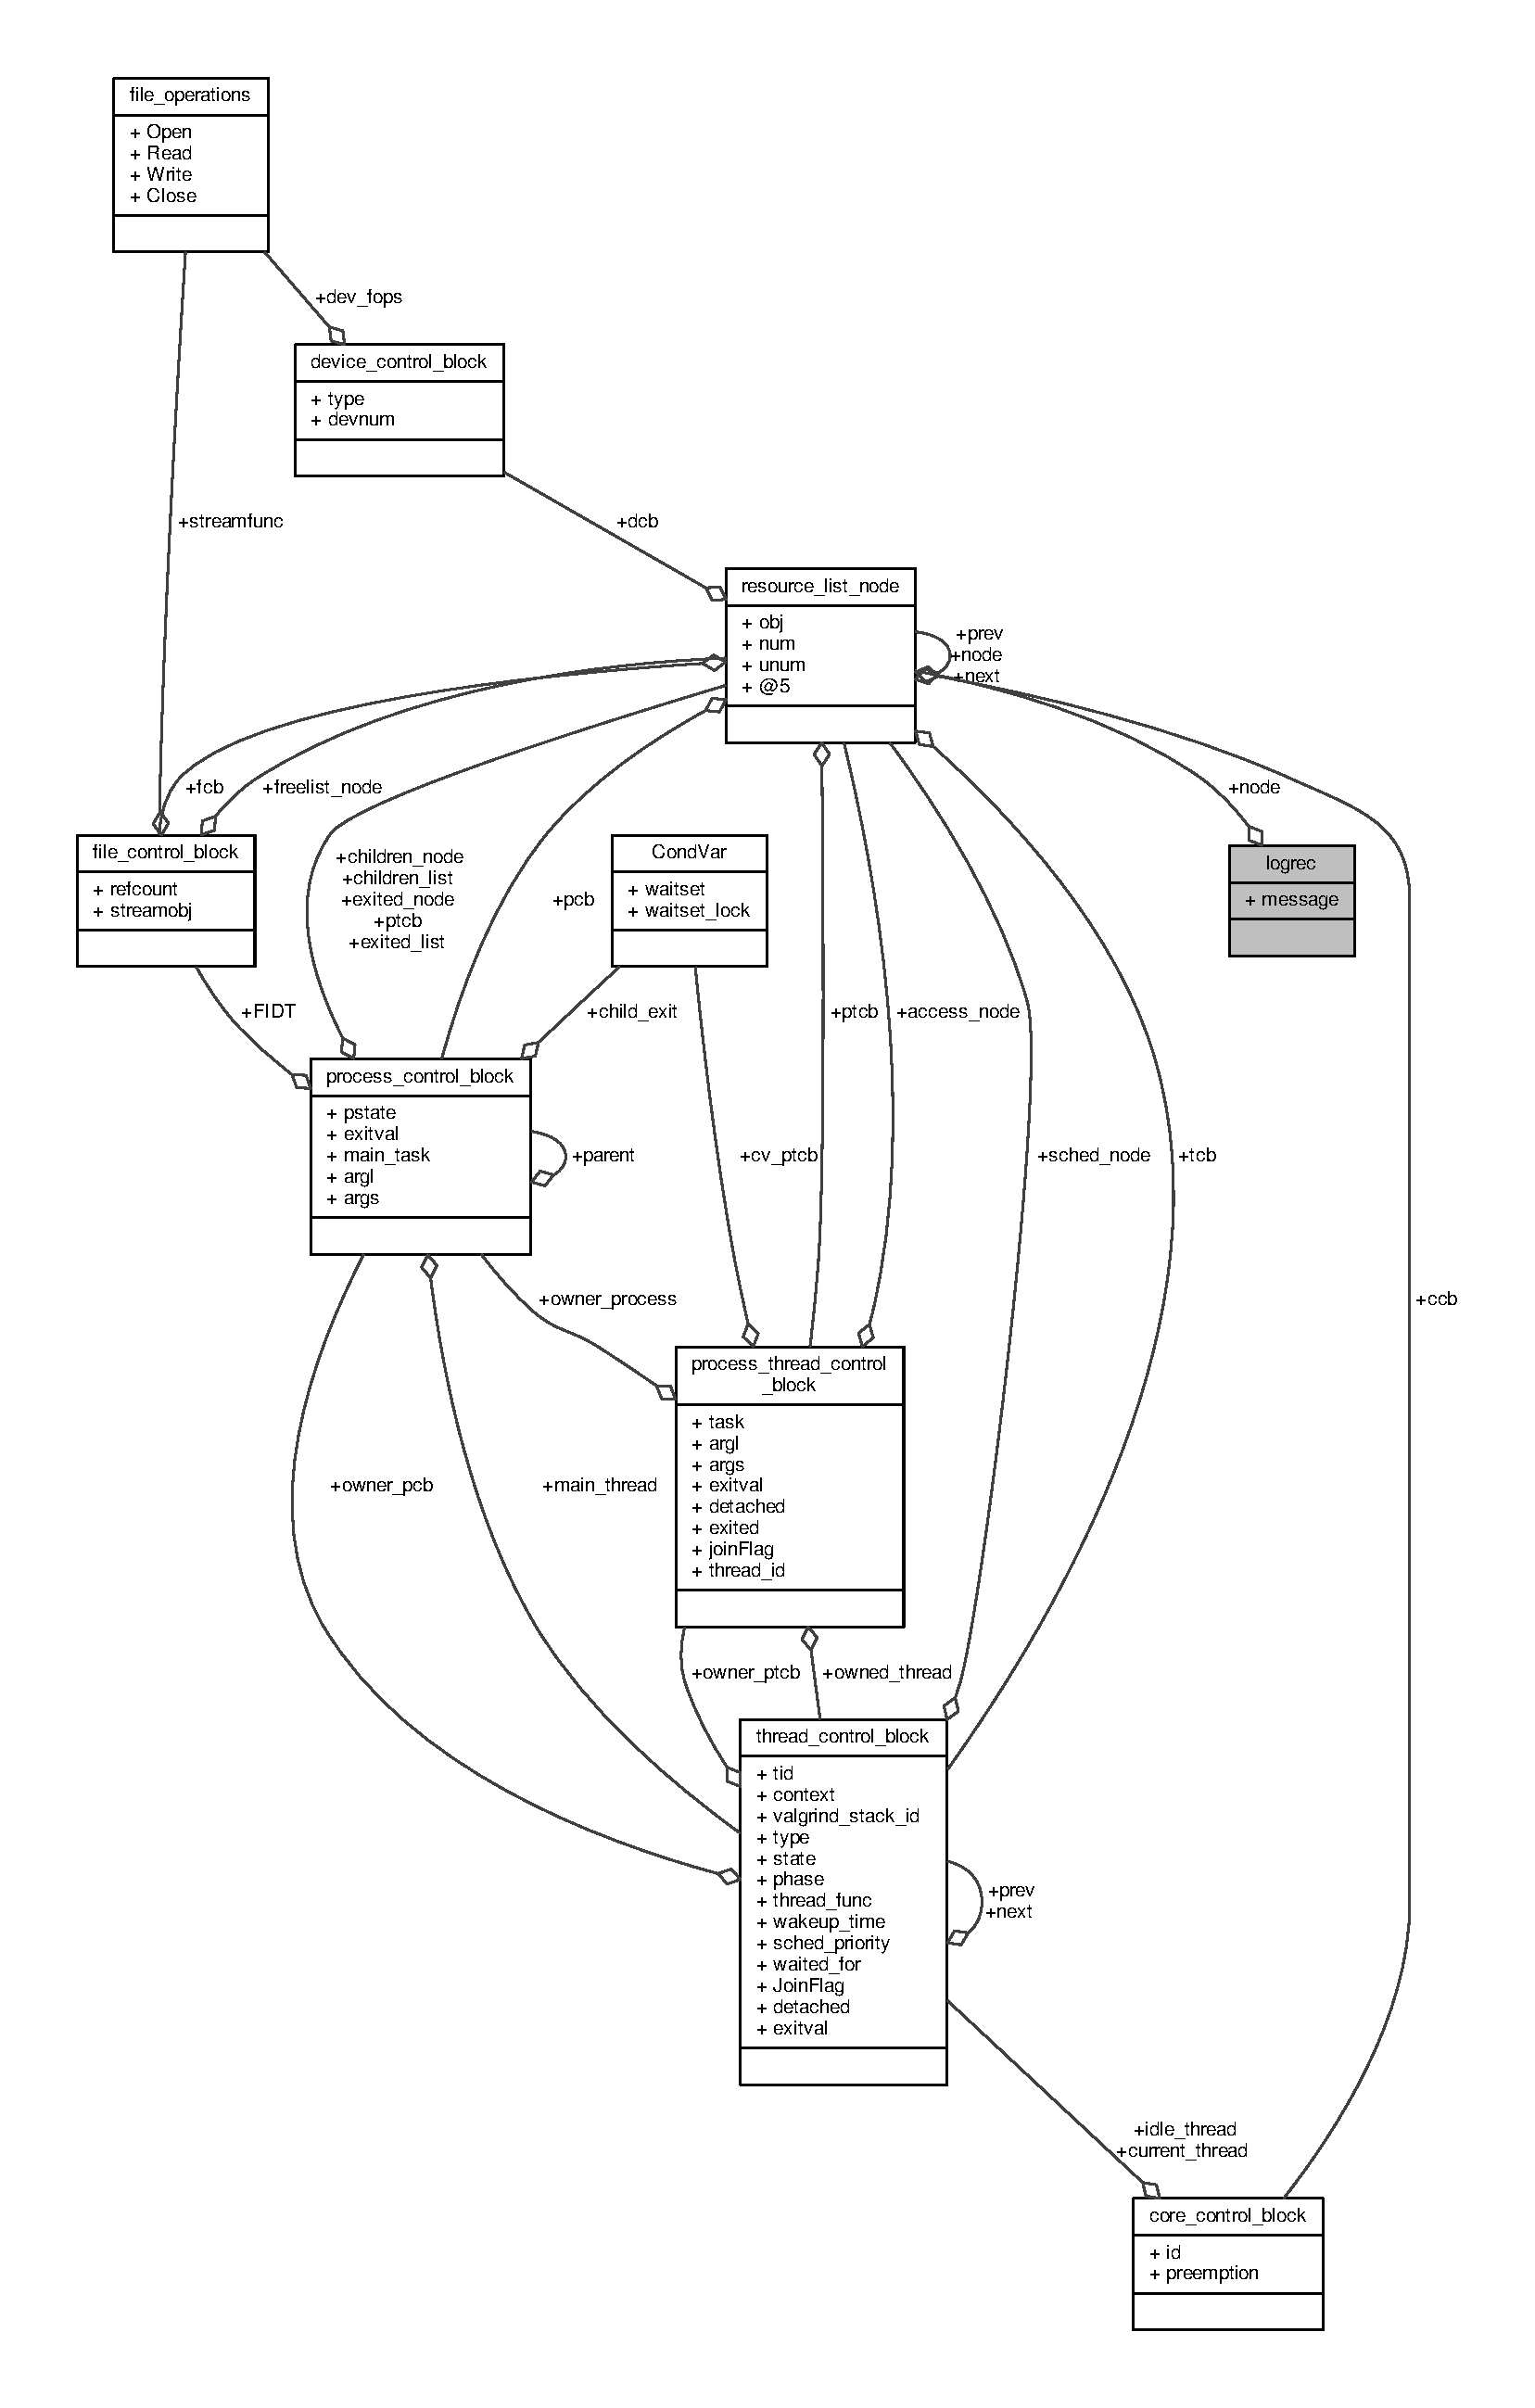
\includegraphics[width=350pt]{structlogrec__coll__graph}
\end{center}
\end{figure}
\subsection*{Data Fields}
\begin{DoxyCompactItemize}
\item 
\hyperlink{group__rlists_ga8f6244877f7ce2322c90525217ea6e7a}{rlnode} {\bfseries node}\hypertarget{structlogrec_ab1f7006e72b67ba7b9d0b26713997aa5}{}\label{structlogrec_ab1f7006e72b67ba7b9d0b26713997aa5}

\item 
char {\bfseries message} \mbox{[}0\mbox{]}\hypertarget{structlogrec_ad21f53e0393fccb77219c1d9d94b7d23}{}\label{structlogrec_ad21f53e0393fccb77219c1d9d94b7d23}

\end{DoxyCompactItemize}


\subsection{Detailed Description}


Definition at line 554 of file tinyos\+\_\+shell.\+c.



The documentation for this struct was generated from the following file\+:\begin{DoxyCompactItemize}
\item 
tinyos\+\_\+shell.\+c\end{DoxyCompactItemize}

\hypertarget{structpeer__variables}{}\section{peer\+\_\+variables Struct Reference}
\label{structpeer__variables}\index{peer\+\_\+variables@{peer\+\_\+variables}}


Collaboration diagram for peer\+\_\+variables\+:\nopagebreak
\begin{figure}[H]
\begin{center}
\leavevmode
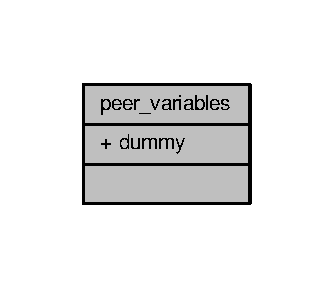
\includegraphics[width=160pt]{structpeer__variables__coll__graph}
\end{center}
\end{figure}
\subsection*{Data Fields}
\begin{DoxyCompactItemize}
\item 
int {\bfseries dummy}\hypertarget{structpeer__variables_a55ff961c263956f40e65d05756672709}{}\label{structpeer__variables_a55ff961c263956f40e65d05756672709}

\end{DoxyCompactItemize}


\subsection{Detailed Description}


Definition at line 23 of file kernel\+\_\+socket.\+c.



The documentation for this struct was generated from the following file\+:\begin{DoxyCompactItemize}
\item 
kernel\+\_\+socket.\+c\end{DoxyCompactItemize}

\hypertarget{structpipe__control__block}{}\section{pipe\+\_\+control\+\_\+block Struct Reference}
\label{structpipe__control__block}\index{pipe\+\_\+control\+\_\+block@{pipe\+\_\+control\+\_\+block}}


Collaboration diagram for pipe\+\_\+control\+\_\+block\+:\nopagebreak
\begin{figure}[H]
\begin{center}
\leavevmode
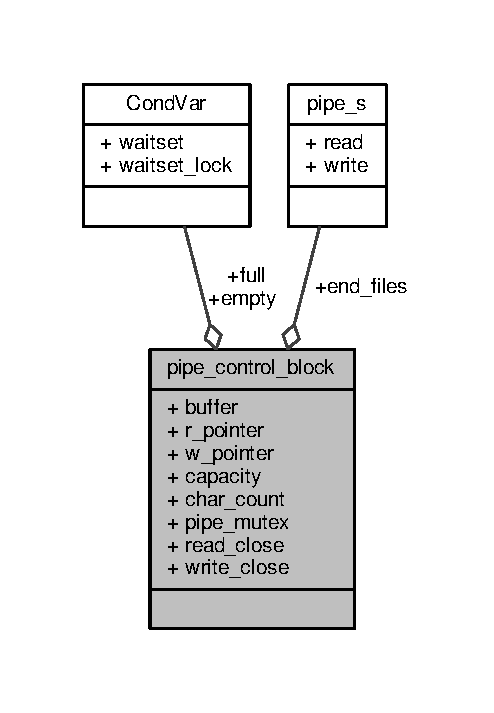
\includegraphics[width=237pt]{structpipe__control__block__coll__graph}
\end{center}
\end{figure}
\subsection*{Data Fields}
\begin{DoxyCompactItemize}
\item 
char $\ast$ {\bfseries buffer}\hypertarget{structpipe__control__block_ae583cd3728bd7487f2fe66adddf95d48}{}\label{structpipe__control__block_ae583cd3728bd7487f2fe66adddf95d48}

\item 
int {\bfseries r\+\_\+pointer}\hypertarget{structpipe__control__block_a9f9eaacb72539adf4aaf45b9efd1c74b}{}\label{structpipe__control__block_a9f9eaacb72539adf4aaf45b9efd1c74b}

\item 
int {\bfseries w\+\_\+pointer}\hypertarget{structpipe__control__block_a7d76f171e180ff49a2863d45574ec912}{}\label{structpipe__control__block_a7d76f171e180ff49a2863d45574ec912}

\item 
int {\bfseries capacity}\hypertarget{structpipe__control__block_a4f42a0270d4cf815b031fc6550592e7c}{}\label{structpipe__control__block_a4f42a0270d4cf815b031fc6550592e7c}

\item 
int {\bfseries char\+\_\+count}\hypertarget{structpipe__control__block_af49ccbbfe7302896843a2aa677dd0e60}{}\label{structpipe__control__block_af49ccbbfe7302896843a2aa677dd0e60}

\item 
\hyperlink{group__syscalls_gad56b5ceaaf7d3ab88b4be7f622314dfb}{pipe\+\_\+t} $\ast$ {\bfseries end\+\_\+files}\hypertarget{structpipe__control__block_a43fd0811ef32129a87f5bbafb258bf44}{}\label{structpipe__control__block_a43fd0811ef32129a87f5bbafb258bf44}

\item 
\hyperlink{structCondVar}{Cond\+Var} {\bfseries full}\hypertarget{structpipe__control__block_a7be46f5729d20e6f1483cdb13334cb2a}{}\label{structpipe__control__block_a7be46f5729d20e6f1483cdb13334cb2a}

\item 
\hyperlink{structCondVar}{Cond\+Var} {\bfseries empty}\hypertarget{structpipe__control__block_aaaedddb6ac8ba86e1437a664559496b8}{}\label{structpipe__control__block_aaaedddb6ac8ba86e1437a664559496b8}

\item 
\hyperlink{group__syscalls_gaef2ec62cae8e0031fd19fc8b91083ade}{Mutex} {\bfseries pipe\+\_\+mutex}\hypertarget{structpipe__control__block_a288c5b54d81699cb967cdd1dc133e766}{}\label{structpipe__control__block_a288c5b54d81699cb967cdd1dc133e766}

\item 
short {\bfseries read\+\_\+close}\hypertarget{structpipe__control__block_a056509d00ad11a6c77047753c5e6341d}{}\label{structpipe__control__block_a056509d00ad11a6c77047753c5e6341d}

\item 
short {\bfseries write\+\_\+close}\hypertarget{structpipe__control__block_a92ec2ce12158afe246e0dd378a14a3d0}{}\label{structpipe__control__block_a92ec2ce12158afe246e0dd378a14a3d0}

\end{DoxyCompactItemize}


\subsection{Detailed Description}


Definition at line 132 of file kernel\+\_\+streams.\+h.



The documentation for this struct was generated from the following file\+:\begin{DoxyCompactItemize}
\item 
\hyperlink{kernel__streams_8h}{kernel\+\_\+streams.\+h}\end{DoxyCompactItemize}

\hypertarget{structpipe__s}{}\section{pipe\+\_\+s Struct Reference}
\label{structpipe__s}\index{pipe\+\_\+s@{pipe\+\_\+s}}


A pair of file ids, describing a pipe.  




{\ttfamily \#include $<$tinyos.\+h$>$}



Collaboration diagram for pipe\+\_\+s\+:\nopagebreak
\begin{figure}[H]
\begin{center}
\leavevmode
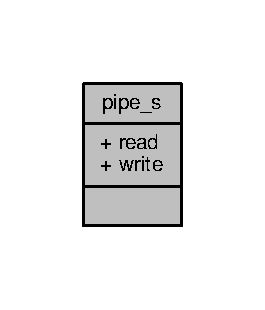
\includegraphics[width=127pt]{structpipe__s__coll__graph}
\end{center}
\end{figure}
\subsection*{Data Fields}
\begin{DoxyCompactItemize}
\item 
\hyperlink{group__syscalls_ga5097222c5f0da97d92d4712359abc38f}{Fid\+\_\+t} \hyperlink{structpipe__s_ad0839b4f9b1fdb0241411952203f18aa}{read}
\item 
\hyperlink{group__syscalls_ga5097222c5f0da97d92d4712359abc38f}{Fid\+\_\+t} \hyperlink{structpipe__s_a69acc9cdf5f10195c43491e3ffa98cb1}{write}
\end{DoxyCompactItemize}


\subsection{Detailed Description}
A pair of file ids, describing a pipe. 

This structure is initialized by the {\ttfamily \hyperlink{group__syscalls_gab6355ce54e047c31538ed5ed9108b5b3}{Pipe()}} system call with two file descriptors, for the read and write ends of the pipe respectively. Writing bytes to the write end using {\ttfamily \hyperlink{group__syscalls_gaf046f003fde24f79fb395c250137856c}{Write()}} will make them available at the read end, unsing {\ttfamily \hyperlink{group__syscalls_ga3e9dc545a789eb45b2d356eabbac3ee3}{Read()}}. 

Definition at line 508 of file tinyos.\+h.



\subsection{Field Documentation}
\index{pipe\+\_\+s@{pipe\+\_\+s}!read@{read}}
\index{read@{read}!pipe\+\_\+s@{pipe\+\_\+s}}
\subsubsection[{\texorpdfstring{read}{read}}]{\setlength{\rightskip}{0pt plus 5cm}{\bf Fid\+\_\+t} pipe\+\_\+s\+::read}\hypertarget{structpipe__s_ad0839b4f9b1fdb0241411952203f18aa}{}\label{structpipe__s_ad0839b4f9b1fdb0241411952203f18aa}
The read end of the pipe 

Definition at line 509 of file tinyos.\+h.

\index{pipe\+\_\+s@{pipe\+\_\+s}!write@{write}}
\index{write@{write}!pipe\+\_\+s@{pipe\+\_\+s}}
\subsubsection[{\texorpdfstring{write}{write}}]{\setlength{\rightskip}{0pt plus 5cm}{\bf Fid\+\_\+t} pipe\+\_\+s\+::write}\hypertarget{structpipe__s_a69acc9cdf5f10195c43491e3ffa98cb1}{}\label{structpipe__s_a69acc9cdf5f10195c43491e3ffa98cb1}
The write end of the pipe 

Definition at line 510 of file tinyos.\+h.



The documentation for this struct was generated from the following file\+:\begin{DoxyCompactItemize}
\item 
\hyperlink{tinyos_8h}{tinyos.\+h}\end{DoxyCompactItemize}

\hypertarget{structport__control__block}{}\section{port\+\_\+control\+\_\+block Struct Reference}
\label{structport__control__block}\index{port\+\_\+control\+\_\+block@{port\+\_\+control\+\_\+block}}


Collaboration diagram for port\+\_\+control\+\_\+block\+:
\nopagebreak
\begin{figure}[H]
\begin{center}
\leavevmode
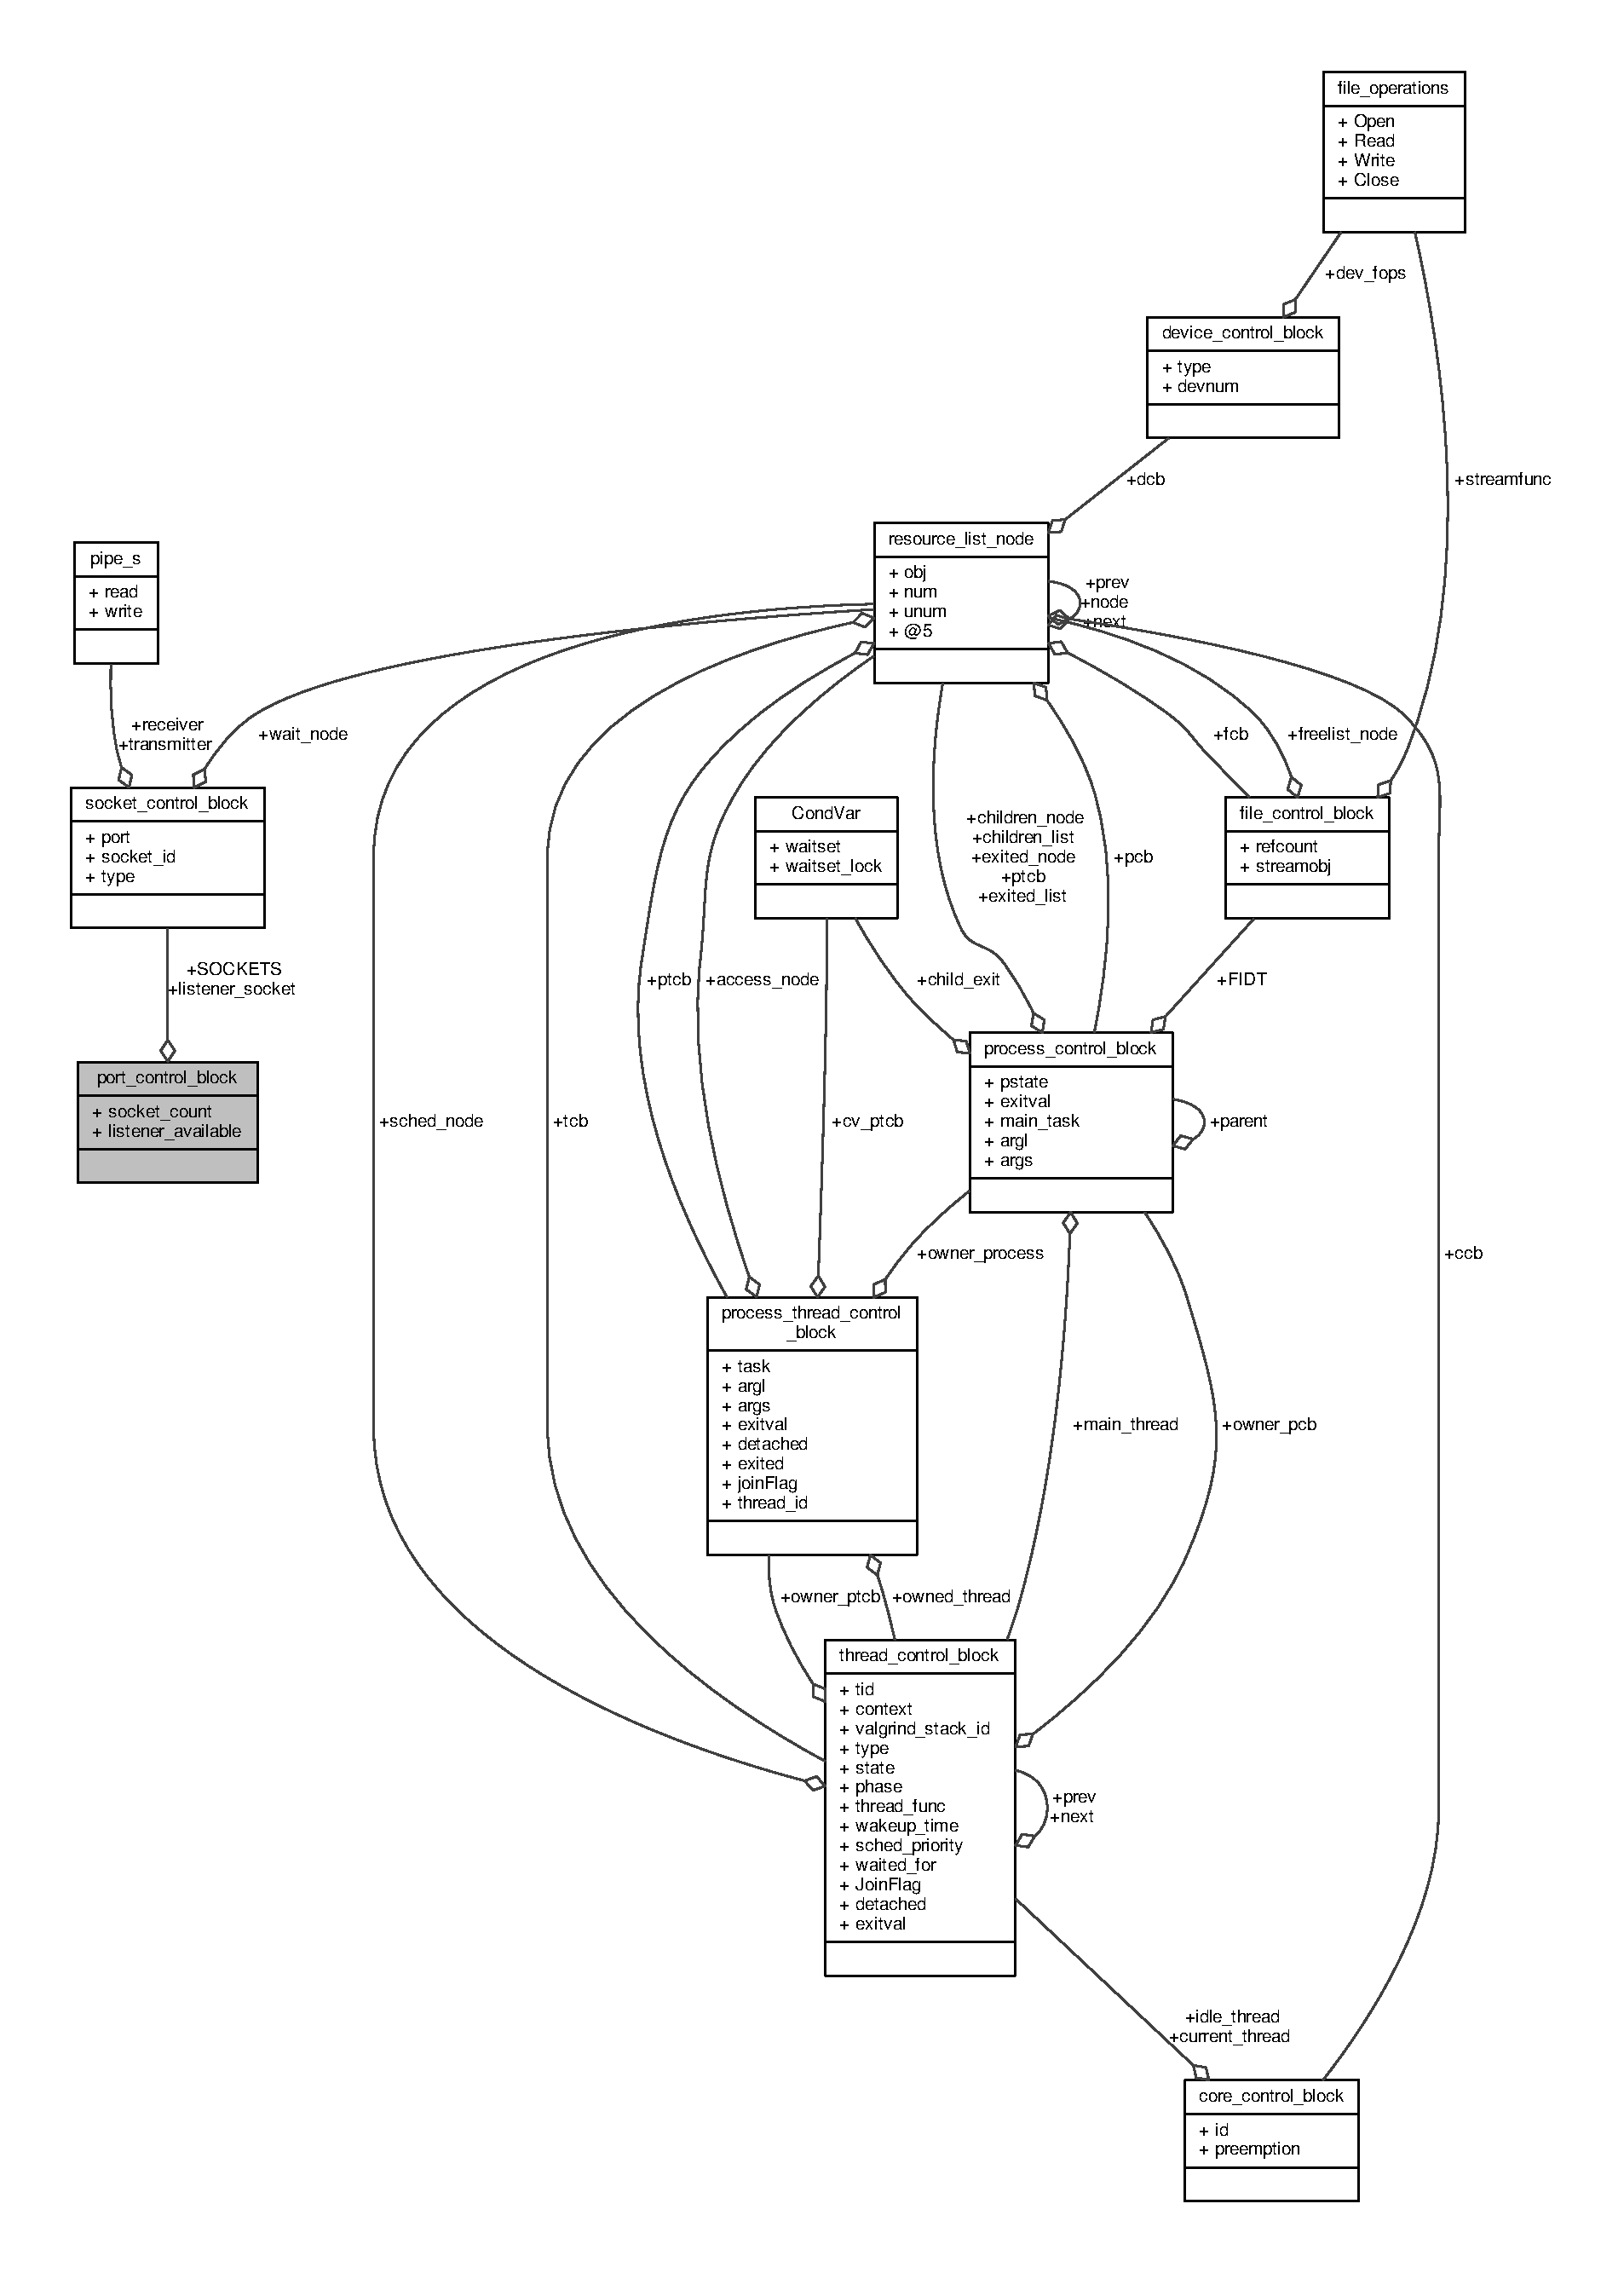
\includegraphics[width=350pt]{structport__control__block__coll__graph}
\end{center}
\end{figure}
\subsection*{Data Fields}
\begin{DoxyCompactItemize}
\item 
unsigned int {\bfseries socket\+\_\+count}\hypertarget{structport__control__block_a0360f6071ffc42ff4f050503faaf1bee}{}\label{structport__control__block_a0360f6071ffc42ff4f050503faaf1bee}

\item 
\hyperlink{structsocket__control__block}{S\+CB} $\ast$ {\bfseries S\+O\+C\+K\+E\+TS} \mbox{[}M\+A\+X\+\_\+\+S\+O\+C\+K\+E\+TS\mbox{]}\hypertarget{structport__control__block_a8351d320913a09d106738415102038cf}{}\label{structport__control__block_a8351d320913a09d106738415102038cf}

\item 
\hyperlink{structsocket__control__block}{S\+CB} $\ast$ {\bfseries listener\+\_\+socket}\hypertarget{structport__control__block_a0843e286af579c2a85f6ef59768f2c40}{}\label{structport__control__block_a0843e286af579c2a85f6ef59768f2c40}

\item 
short {\bfseries listener\+\_\+available}\hypertarget{structport__control__block_aabbaa06dd8e23b31baeb8910f78caee3}{}\label{structport__control__block_aabbaa06dd8e23b31baeb8910f78caee3}

\end{DoxyCompactItemize}


\subsection{Detailed Description}


Definition at line 48 of file kernel\+\_\+socket.\+c.



The documentation for this struct was generated from the following file\+:\begin{DoxyCompactItemize}
\item 
kernel\+\_\+socket.\+c\end{DoxyCompactItemize}

\hypertarget{structprocess__control__block}{}\section{process\+\_\+control\+\_\+block Struct Reference}
\label{structprocess__control__block}\index{process\+\_\+control\+\_\+block@{process\+\_\+control\+\_\+block}}


Process Control Block.  




{\ttfamily \#include $<$kernel\+\_\+proc.\+h$>$}



Collaboration diagram for process\+\_\+control\+\_\+block\+:
\nopagebreak
\begin{figure}[H]
\begin{center}
\leavevmode
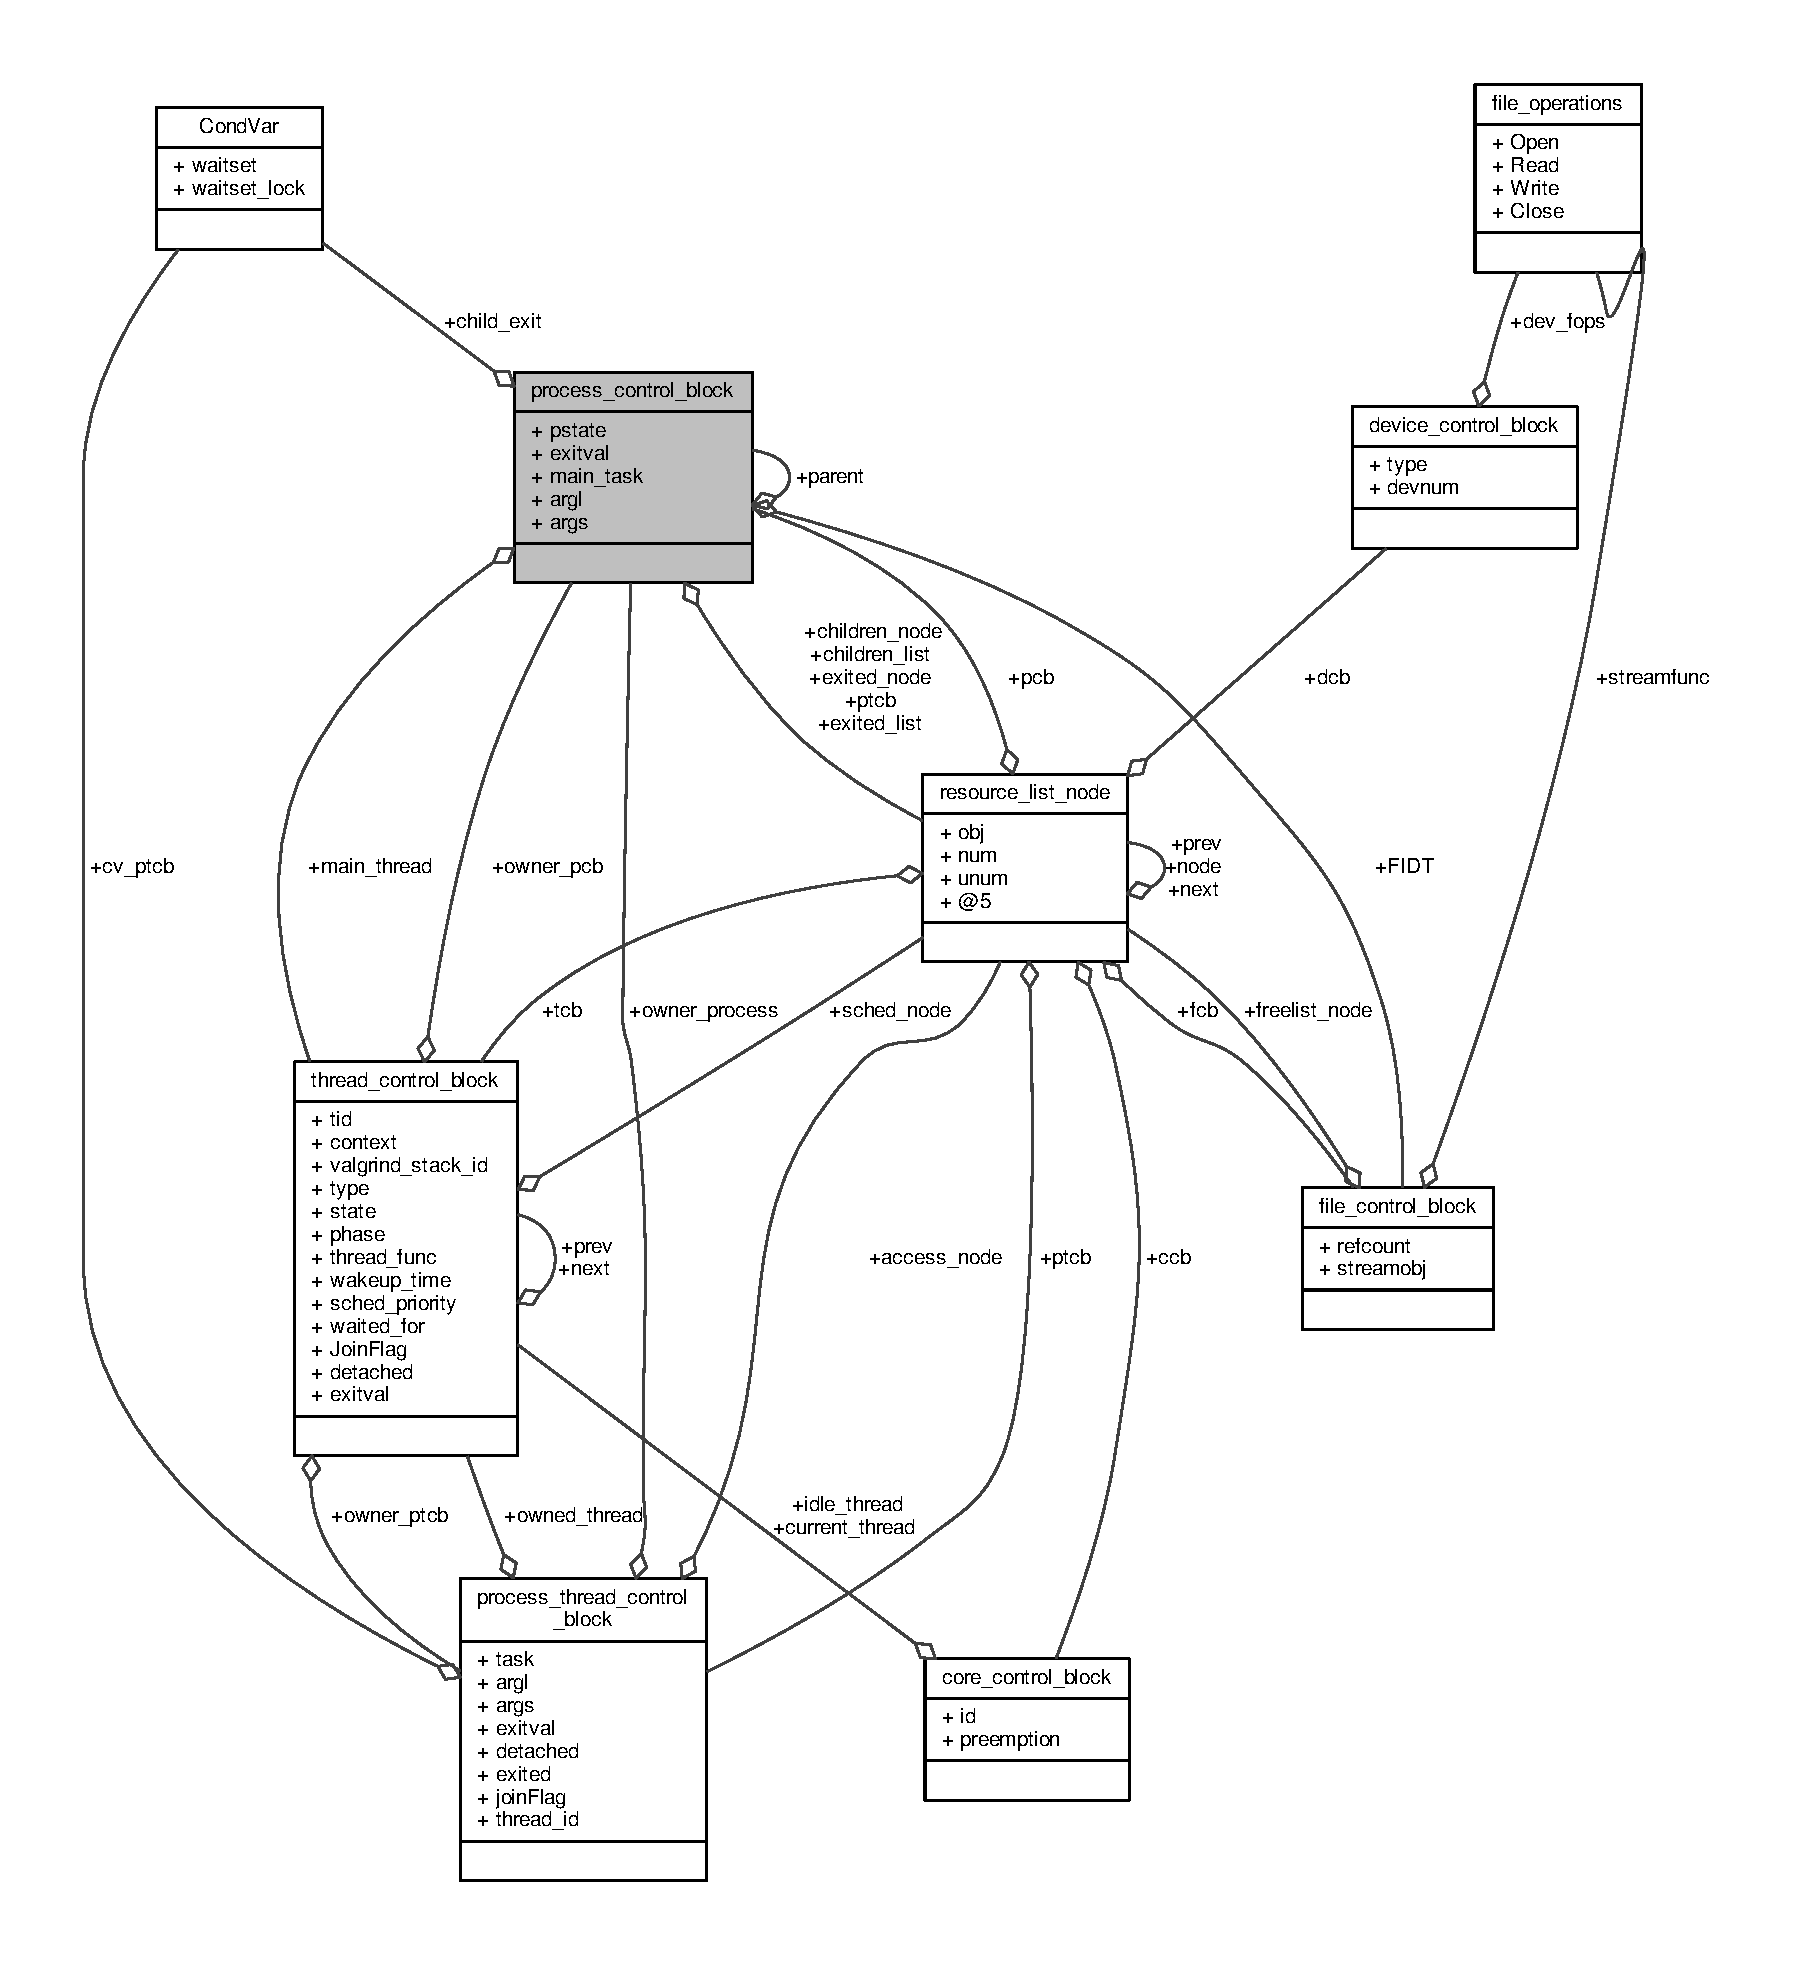
\includegraphics[width=350pt]{structprocess__control__block__coll__graph}
\end{center}
\end{figure}
\subsection*{Data Fields}
\begin{DoxyCompactItemize}
\item 
\hyperlink{group__proc_gade1eea4d20492c4c97263201145e5097}{pid\+\_\+state} \hyperlink{structprocess__control__block_ae3334dd8a5747f108124c7129c27eea5}{pstate}
\item 
\hyperlink{group__proc_ga91aaadf0c3f9cef2293a99c69795323f}{P\+CB} $\ast$ \hyperlink{structprocess__control__block_af20d0c36862c6def80024b4586ff8934}{parent}
\item 
int \hyperlink{structprocess__control__block_add9b4f6d506a3538be7b53411e94fd28}{exitval}
\item 
\hyperlink{group__scheduler_gaf88d9c946bf70b36a1e8bc34383abfc9}{T\+CB} $\ast$ \hyperlink{structprocess__control__block_a3b7a2a952ec5c19d7331307639c78482}{main\+\_\+thread}
\item 
\hyperlink{group__syscalls_gaec3f2f835e105271fbbc00272c0ba984}{Task} \hyperlink{structprocess__control__block_a7d4ddbf8f67ac2bfe9774796b818354e}{main\+\_\+task}
\item 
int \hyperlink{structprocess__control__block_a8c8667a0f61f4380b3d5c69c57315511}{argl}
\item 
void $\ast$ \hyperlink{structprocess__control__block_af7ac33b69a8a1dc582e0fa35cc90568a}{args}
\item 
\hyperlink{group__rlists_ga8f6244877f7ce2322c90525217ea6e7a}{rlnode} \hyperlink{structprocess__control__block_a79b0dd70bbfff1d7da6ab4cbbd00eb1f}{children\+\_\+list}
\item 
\hyperlink{group__rlists_ga8f6244877f7ce2322c90525217ea6e7a}{rlnode} \hyperlink{structprocess__control__block_afddb936103b136214462e1ed870c4c70}{exited\+\_\+list}
\item 
\hyperlink{group__rlists_ga8f6244877f7ce2322c90525217ea6e7a}{rlnode} \hyperlink{structprocess__control__block_a5b9aeabcc3d676cda39eb563a4cc5bd9}{children\+\_\+node}
\item 
\hyperlink{group__rlists_ga8f6244877f7ce2322c90525217ea6e7a}{rlnode} \hyperlink{structprocess__control__block_a9e0d93783a89bd92f39243353f04a27e}{exited\+\_\+node}
\item 
\hyperlink{structCondVar}{Cond\+Var} \hyperlink{structprocess__control__block_a6bcb52e96fdf96d060af2b11f07d44bd}{child\+\_\+exit}
\item 
\hyperlink{group__streams_ga0c7e751afb9d6cadebf070961804d400}{F\+CB} $\ast$ \hyperlink{structprocess__control__block_aad72d85bd79a3100a497d11630a38977}{F\+I\+DT} \mbox{[}\hyperlink{group__syscalls_ga9c697bf9e856897ad75f28190a6f0b68}{M\+A\+X\+\_\+\+F\+I\+L\+E\+ID}\mbox{]}
\item 
\hyperlink{group__rlists_ga8f6244877f7ce2322c90525217ea6e7a}{rlnode} {\bfseries ptcb}\hypertarget{structprocess__control__block_a8fe369a32ad6bc5e27a2e1b5784e43c0}{}\label{structprocess__control__block_a8fe369a32ad6bc5e27a2e1b5784e43c0}

\end{DoxyCompactItemize}


\subsection{Detailed Description}
Process Control Block. 

This structure holds all information pertaining to a process. 

Definition at line 38 of file kernel\+\_\+proc.\+h.



\subsection{Field Documentation}
\index{process\+\_\+control\+\_\+block@{process\+\_\+control\+\_\+block}!argl@{argl}}
\index{argl@{argl}!process\+\_\+control\+\_\+block@{process\+\_\+control\+\_\+block}}
\subsubsection[{\texorpdfstring{argl}{argl}}]{\setlength{\rightskip}{0pt plus 5cm}int process\+\_\+control\+\_\+block\+::argl}\hypertarget{structprocess__control__block_a8c8667a0f61f4380b3d5c69c57315511}{}\label{structprocess__control__block_a8c8667a0f61f4380b3d5c69c57315511}
The main thread\textquotesingle{}s argument length 

Definition at line 46 of file kernel\+\_\+proc.\+h.

\index{process\+\_\+control\+\_\+block@{process\+\_\+control\+\_\+block}!args@{args}}
\index{args@{args}!process\+\_\+control\+\_\+block@{process\+\_\+control\+\_\+block}}
\subsubsection[{\texorpdfstring{args}{args}}]{\setlength{\rightskip}{0pt plus 5cm}void$\ast$ process\+\_\+control\+\_\+block\+::args}\hypertarget{structprocess__control__block_af7ac33b69a8a1dc582e0fa35cc90568a}{}\label{structprocess__control__block_af7ac33b69a8a1dc582e0fa35cc90568a}
The main thread\textquotesingle{}s argument string 

Definition at line 47 of file kernel\+\_\+proc.\+h.

\index{process\+\_\+control\+\_\+block@{process\+\_\+control\+\_\+block}!child\+\_\+exit@{child\+\_\+exit}}
\index{child\+\_\+exit@{child\+\_\+exit}!process\+\_\+control\+\_\+block@{process\+\_\+control\+\_\+block}}
\subsubsection[{\texorpdfstring{child\+\_\+exit}{child_exit}}]{\setlength{\rightskip}{0pt plus 5cm}{\bf Cond\+Var} process\+\_\+control\+\_\+block\+::child\+\_\+exit}\hypertarget{structprocess__control__block_a6bcb52e96fdf96d060af2b11f07d44bd}{}\label{structprocess__control__block_a6bcb52e96fdf96d060af2b11f07d44bd}
Condition variable for {\ttfamily Wait\+Child} 

Definition at line 54 of file kernel\+\_\+proc.\+h.

\index{process\+\_\+control\+\_\+block@{process\+\_\+control\+\_\+block}!children\+\_\+list@{children\+\_\+list}}
\index{children\+\_\+list@{children\+\_\+list}!process\+\_\+control\+\_\+block@{process\+\_\+control\+\_\+block}}
\subsubsection[{\texorpdfstring{children\+\_\+list}{children_list}}]{\setlength{\rightskip}{0pt plus 5cm}{\bf rlnode} process\+\_\+control\+\_\+block\+::children\+\_\+list}\hypertarget{structprocess__control__block_a79b0dd70bbfff1d7da6ab4cbbd00eb1f}{}\label{structprocess__control__block_a79b0dd70bbfff1d7da6ab4cbbd00eb1f}
List of children 

Definition at line 49 of file kernel\+\_\+proc.\+h.

\index{process\+\_\+control\+\_\+block@{process\+\_\+control\+\_\+block}!children\+\_\+node@{children\+\_\+node}}
\index{children\+\_\+node@{children\+\_\+node}!process\+\_\+control\+\_\+block@{process\+\_\+control\+\_\+block}}
\subsubsection[{\texorpdfstring{children\+\_\+node}{children_node}}]{\setlength{\rightskip}{0pt plus 5cm}{\bf rlnode} process\+\_\+control\+\_\+block\+::children\+\_\+node}\hypertarget{structprocess__control__block_a5b9aeabcc3d676cda39eb563a4cc5bd9}{}\label{structprocess__control__block_a5b9aeabcc3d676cda39eb563a4cc5bd9}
Intrusive node for {\ttfamily children\+\_\+list} 

Definition at line 51 of file kernel\+\_\+proc.\+h.

\index{process\+\_\+control\+\_\+block@{process\+\_\+control\+\_\+block}!exited\+\_\+list@{exited\+\_\+list}}
\index{exited\+\_\+list@{exited\+\_\+list}!process\+\_\+control\+\_\+block@{process\+\_\+control\+\_\+block}}
\subsubsection[{\texorpdfstring{exited\+\_\+list}{exited_list}}]{\setlength{\rightskip}{0pt plus 5cm}{\bf rlnode} process\+\_\+control\+\_\+block\+::exited\+\_\+list}\hypertarget{structprocess__control__block_afddb936103b136214462e1ed870c4c70}{}\label{structprocess__control__block_afddb936103b136214462e1ed870c4c70}
List of exited children 

Definition at line 50 of file kernel\+\_\+proc.\+h.

\index{process\+\_\+control\+\_\+block@{process\+\_\+control\+\_\+block}!exited\+\_\+node@{exited\+\_\+node}}
\index{exited\+\_\+node@{exited\+\_\+node}!process\+\_\+control\+\_\+block@{process\+\_\+control\+\_\+block}}
\subsubsection[{\texorpdfstring{exited\+\_\+node}{exited_node}}]{\setlength{\rightskip}{0pt plus 5cm}{\bf rlnode} process\+\_\+control\+\_\+block\+::exited\+\_\+node}\hypertarget{structprocess__control__block_a9e0d93783a89bd92f39243353f04a27e}{}\label{structprocess__control__block_a9e0d93783a89bd92f39243353f04a27e}
Intrusive node for {\ttfamily exited\+\_\+list} 

Definition at line 52 of file kernel\+\_\+proc.\+h.

\index{process\+\_\+control\+\_\+block@{process\+\_\+control\+\_\+block}!exitval@{exitval}}
\index{exitval@{exitval}!process\+\_\+control\+\_\+block@{process\+\_\+control\+\_\+block}}
\subsubsection[{\texorpdfstring{exitval}{exitval}}]{\setlength{\rightskip}{0pt plus 5cm}int process\+\_\+control\+\_\+block\+::exitval}\hypertarget{structprocess__control__block_add9b4f6d506a3538be7b53411e94fd28}{}\label{structprocess__control__block_add9b4f6d506a3538be7b53411e94fd28}
The exit value 

Definition at line 42 of file kernel\+\_\+proc.\+h.

\index{process\+\_\+control\+\_\+block@{process\+\_\+control\+\_\+block}!F\+I\+DT@{F\+I\+DT}}
\index{F\+I\+DT@{F\+I\+DT}!process\+\_\+control\+\_\+block@{process\+\_\+control\+\_\+block}}
\subsubsection[{\texorpdfstring{F\+I\+DT}{FIDT}}]{\setlength{\rightskip}{0pt plus 5cm}{\bf F\+CB}$\ast$ process\+\_\+control\+\_\+block\+::\+F\+I\+DT\mbox{[}{\bf M\+A\+X\+\_\+\+F\+I\+L\+E\+ID}\mbox{]}}\hypertarget{structprocess__control__block_aad72d85bd79a3100a497d11630a38977}{}\label{structprocess__control__block_aad72d85bd79a3100a497d11630a38977}
The fileid table of the process 

Definition at line 56 of file kernel\+\_\+proc.\+h.

\index{process\+\_\+control\+\_\+block@{process\+\_\+control\+\_\+block}!main\+\_\+task@{main\+\_\+task}}
\index{main\+\_\+task@{main\+\_\+task}!process\+\_\+control\+\_\+block@{process\+\_\+control\+\_\+block}}
\subsubsection[{\texorpdfstring{main\+\_\+task}{main_task}}]{\setlength{\rightskip}{0pt plus 5cm}{\bf Task} process\+\_\+control\+\_\+block\+::main\+\_\+task}\hypertarget{structprocess__control__block_a7d4ddbf8f67ac2bfe9774796b818354e}{}\label{structprocess__control__block_a7d4ddbf8f67ac2bfe9774796b818354e}
The main thread\textquotesingle{}s function 

Definition at line 45 of file kernel\+\_\+proc.\+h.

\index{process\+\_\+control\+\_\+block@{process\+\_\+control\+\_\+block}!main\+\_\+thread@{main\+\_\+thread}}
\index{main\+\_\+thread@{main\+\_\+thread}!process\+\_\+control\+\_\+block@{process\+\_\+control\+\_\+block}}
\subsubsection[{\texorpdfstring{main\+\_\+thread}{main_thread}}]{\setlength{\rightskip}{0pt plus 5cm}{\bf T\+CB}$\ast$ process\+\_\+control\+\_\+block\+::main\+\_\+thread}\hypertarget{structprocess__control__block_a3b7a2a952ec5c19d7331307639c78482}{}\label{structprocess__control__block_a3b7a2a952ec5c19d7331307639c78482}
The main thread 

Definition at line 44 of file kernel\+\_\+proc.\+h.

\index{process\+\_\+control\+\_\+block@{process\+\_\+control\+\_\+block}!parent@{parent}}
\index{parent@{parent}!process\+\_\+control\+\_\+block@{process\+\_\+control\+\_\+block}}
\subsubsection[{\texorpdfstring{parent}{parent}}]{\setlength{\rightskip}{0pt plus 5cm}{\bf P\+CB}$\ast$ process\+\_\+control\+\_\+block\+::parent}\hypertarget{structprocess__control__block_af20d0c36862c6def80024b4586ff8934}{}\label{structprocess__control__block_af20d0c36862c6def80024b4586ff8934}
Parent\textquotesingle{}s pcb. 

Definition at line 41 of file kernel\+\_\+proc.\+h.

\index{process\+\_\+control\+\_\+block@{process\+\_\+control\+\_\+block}!pstate@{pstate}}
\index{pstate@{pstate}!process\+\_\+control\+\_\+block@{process\+\_\+control\+\_\+block}}
\subsubsection[{\texorpdfstring{pstate}{pstate}}]{\setlength{\rightskip}{0pt plus 5cm}{\bf pid\+\_\+state} process\+\_\+control\+\_\+block\+::pstate}\hypertarget{structprocess__control__block_ae3334dd8a5747f108124c7129c27eea5}{}\label{structprocess__control__block_ae3334dd8a5747f108124c7129c27eea5}
The pid state for this P\+CB 

Definition at line 39 of file kernel\+\_\+proc.\+h.



The documentation for this struct was generated from the following file\+:\begin{DoxyCompactItemize}
\item 
\hyperlink{kernel__proc_8h}{kernel\+\_\+proc.\+h}\end{DoxyCompactItemize}

\hypertarget{structprocess__thread__control__block}{}\section{process\+\_\+thread\+\_\+control\+\_\+block Struct Reference}
\label{structprocess__thread__control__block}\index{process\+\_\+thread\+\_\+control\+\_\+block@{process\+\_\+thread\+\_\+control\+\_\+block}}


Collaboration diagram for process\+\_\+thread\+\_\+control\+\_\+block\+:
\nopagebreak
\begin{figure}[H]
\begin{center}
\leavevmode
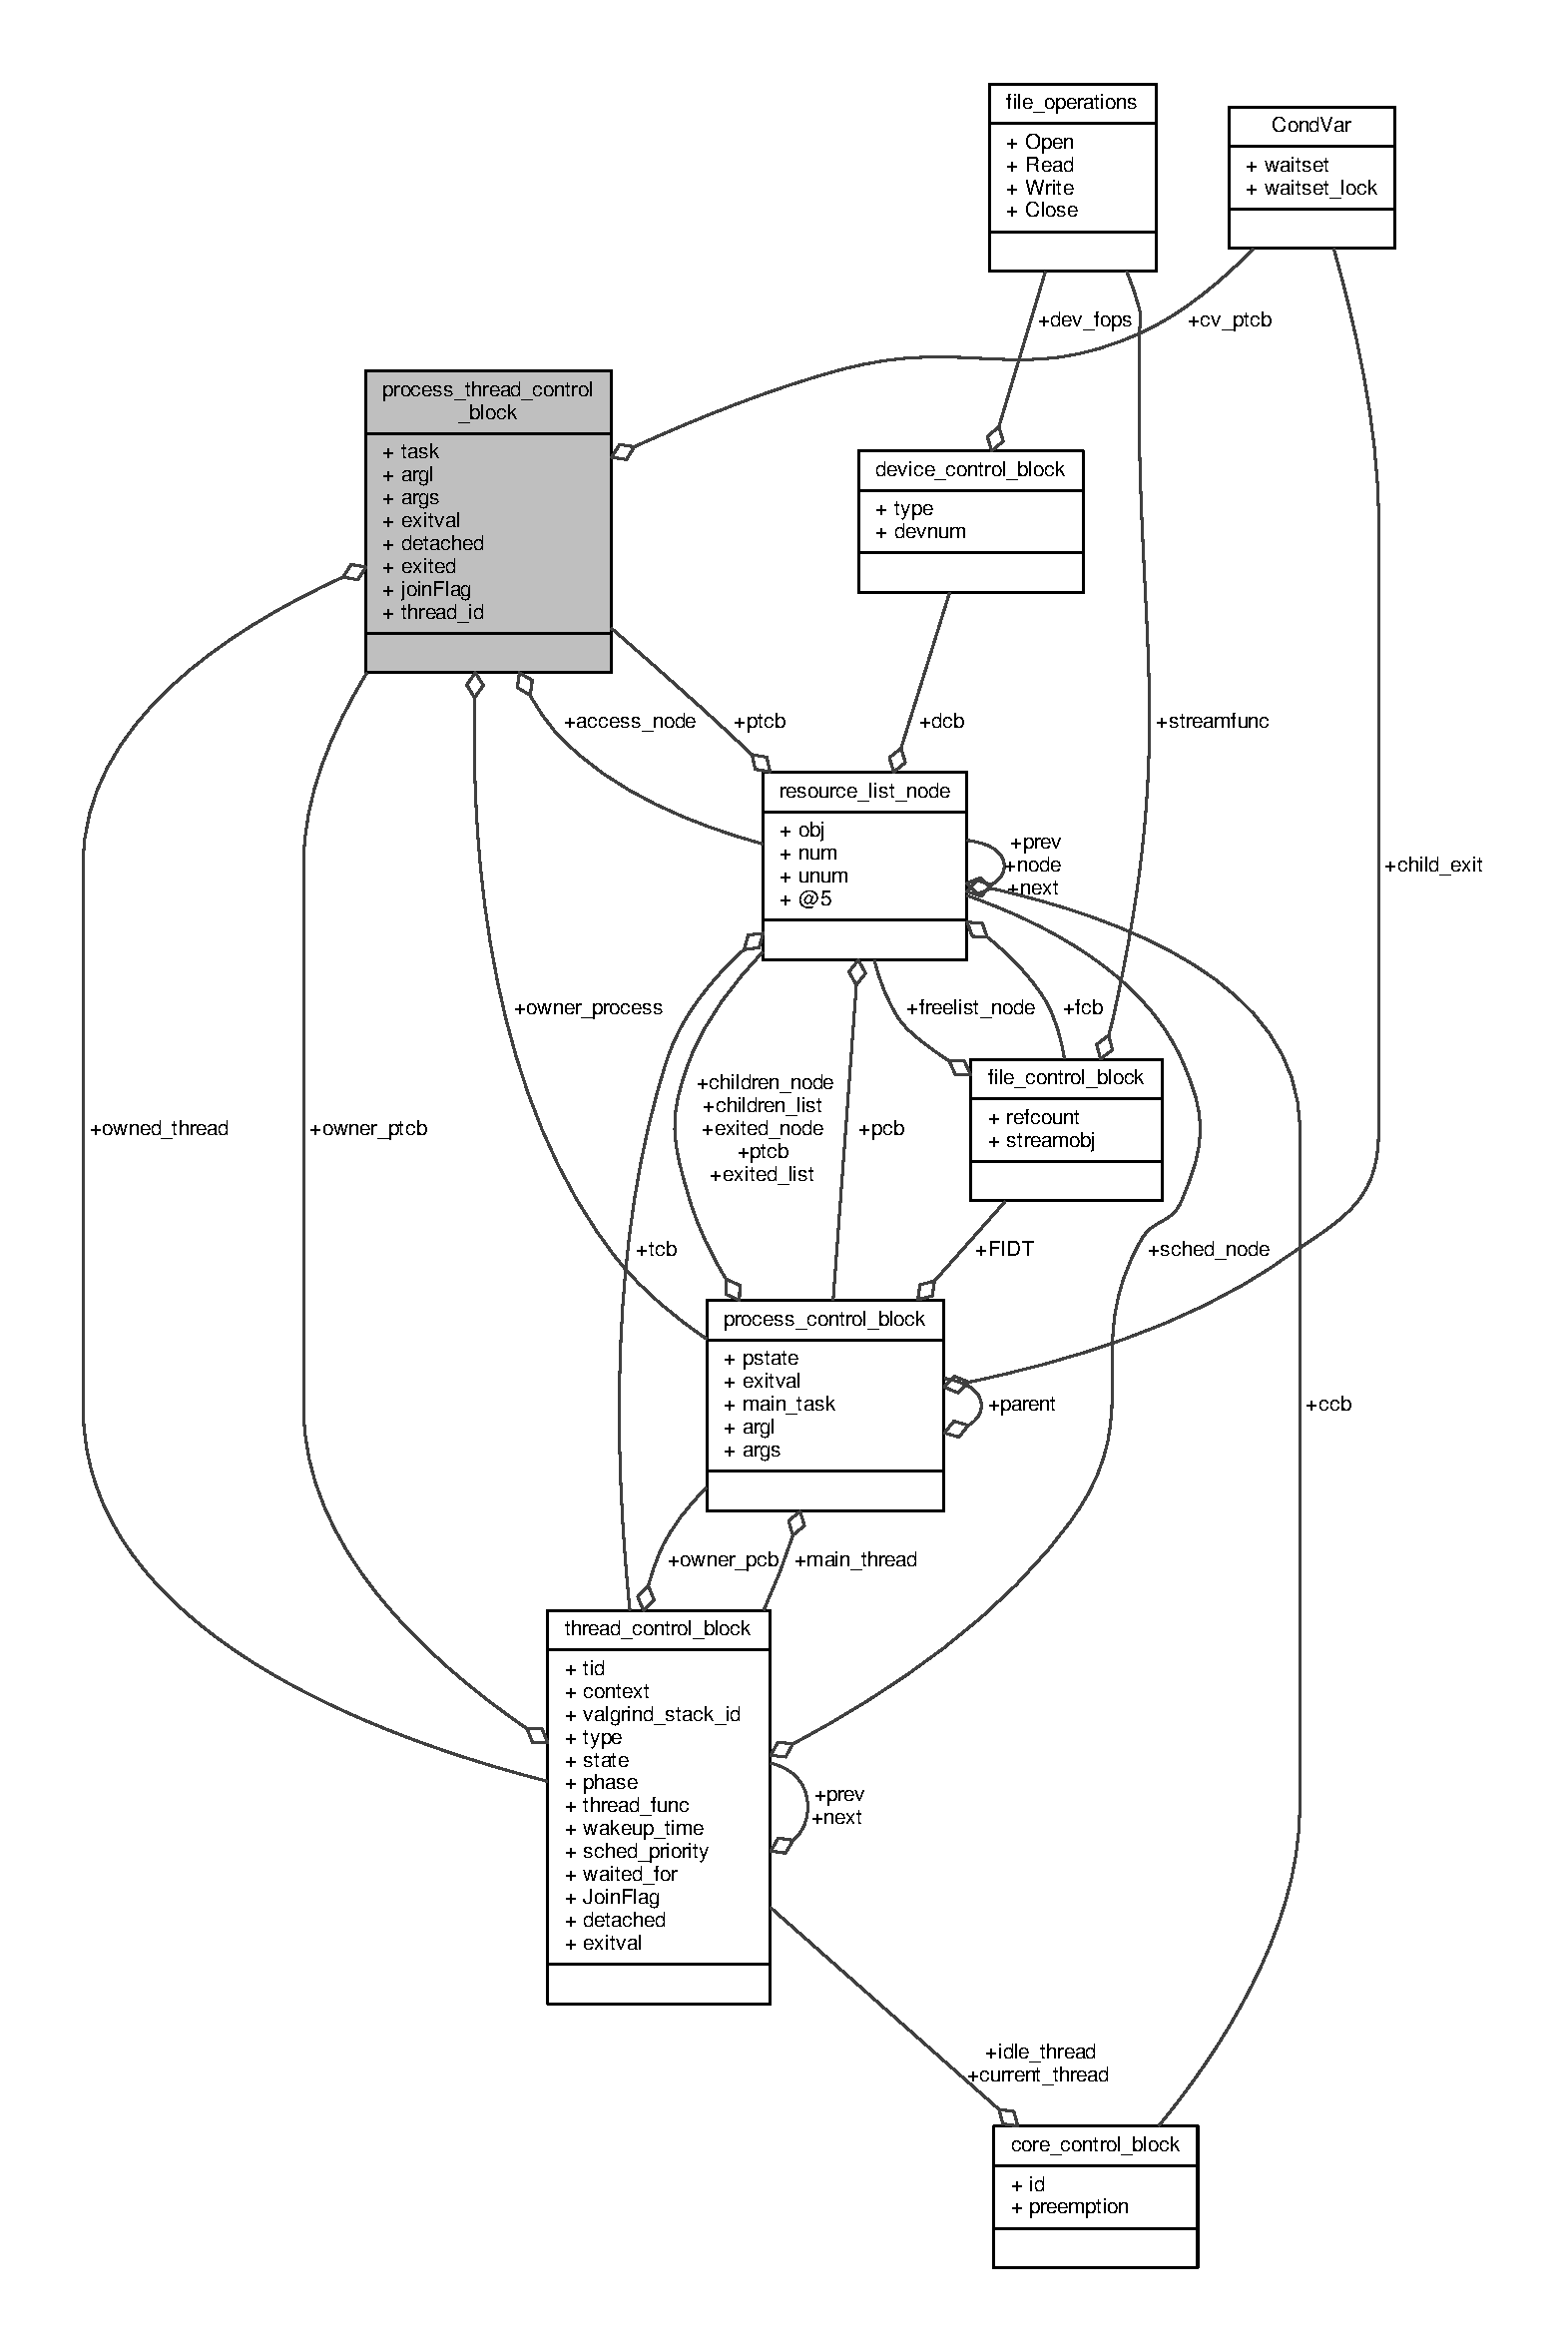
\includegraphics[width=350pt]{structprocess__thread__control__block__coll__graph}
\end{center}
\end{figure}
\subsection*{Data Fields}
\begin{DoxyCompactItemize}
\item 
\hyperlink{group__proc_ga91aaadf0c3f9cef2293a99c69795323f}{P\+CB} $\ast$ {\bfseries owner\+\_\+process}\hypertarget{structprocess__thread__control__block_a040401aaabc78cb50deeeaaa838ccf5e}{}\label{structprocess__thread__control__block_a040401aaabc78cb50deeeaaa838ccf5e}

\item 
\hyperlink{group__scheduler_gaf88d9c946bf70b36a1e8bc34383abfc9}{T\+CB} $\ast$ {\bfseries owned\+\_\+thread}\hypertarget{structprocess__thread__control__block_aa09c0d455e0d9ba3ab13a146a73951e0}{}\label{structprocess__thread__control__block_aa09c0d455e0d9ba3ab13a146a73951e0}

\item 
\hyperlink{group__rlists_ga8f6244877f7ce2322c90525217ea6e7a}{rlnode} {\bfseries access\+\_\+node}\hypertarget{structprocess__thread__control__block_a51f2c0fc0d833033f9fe630743af0167}{}\label{structprocess__thread__control__block_a51f2c0fc0d833033f9fe630743af0167}

\item 
\hyperlink{group__syscalls_gaec3f2f835e105271fbbc00272c0ba984}{Task} {\bfseries task}\hypertarget{structprocess__thread__control__block_a1685f472448d01ec92e39723f37b15fc}{}\label{structprocess__thread__control__block_a1685f472448d01ec92e39723f37b15fc}

\item 
int {\bfseries argl}\hypertarget{structprocess__thread__control__block_afe4baa9de9fc12a689b72c3445b0f024}{}\label{structprocess__thread__control__block_afe4baa9de9fc12a689b72c3445b0f024}

\item 
void $\ast$ {\bfseries args}\hypertarget{structprocess__thread__control__block_a38980424abac6df706714f291678b3ef}{}\label{structprocess__thread__control__block_a38980424abac6df706714f291678b3ef}

\item 
int {\bfseries exitval}\hypertarget{structprocess__thread__control__block_abdf9ff5fef59069e1baa04ee7b5007f6}{}\label{structprocess__thread__control__block_abdf9ff5fef59069e1baa04ee7b5007f6}

\item 
int {\bfseries detached}\hypertarget{structprocess__thread__control__block_aa358c23603b1949eab39bb46d2dc3b2b}{}\label{structprocess__thread__control__block_aa358c23603b1949eab39bb46d2dc3b2b}

\item 
int {\bfseries exited}\hypertarget{structprocess__thread__control__block_a82f3f6173804416baca330d08a0b9a42}{}\label{structprocess__thread__control__block_a82f3f6173804416baca330d08a0b9a42}

\item 
int {\bfseries join\+Flag}\hypertarget{structprocess__thread__control__block_a2621da92c7cf9f63f6fb283d63483a5a}{}\label{structprocess__thread__control__block_a2621da92c7cf9f63f6fb283d63483a5a}

\item 
\hyperlink{group__syscalls_gaf67ad1c55e6b2a79bf8a99106380ce01}{Tid\+\_\+t} {\bfseries thread\+\_\+id}\hypertarget{structprocess__thread__control__block_a0c776905640bee211ddae9a778e5b0df}{}\label{structprocess__thread__control__block_a0c776905640bee211ddae9a778e5b0df}

\item 
\hyperlink{structCondVar}{Cond\+Var} {\bfseries cv\+\_\+ptcb}\hypertarget{structprocess__thread__control__block_a460fe9636de5506fd2aa46348d470650}{}\label{structprocess__thread__control__block_a460fe9636de5506fd2aa46348d470650}

\end{DoxyCompactItemize}


\subsection{Detailed Description}


Definition at line 65 of file kernel\+\_\+proc.\+h.



The documentation for this struct was generated from the following file\+:\begin{DoxyCompactItemize}
\item 
\hyperlink{kernel__proc_8h}{kernel\+\_\+proc.\+h}\end{DoxyCompactItemize}

\hypertarget{structprocinfo}{}\section{procinfo Struct Reference}
\label{structprocinfo}\index{procinfo@{procinfo}}


A struct containing process-\/related information for a non-\/free pid.  




{\ttfamily \#include $<$tinyos.\+h$>$}



Collaboration diagram for procinfo\+:\nopagebreak
\begin{figure}[H]
\begin{center}
\leavevmode
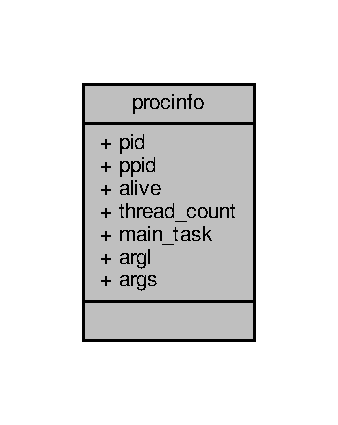
\includegraphics[width=162pt]{structprocinfo__coll__graph}
\end{center}
\end{figure}
\subsection*{Data Fields}
\begin{DoxyCompactItemize}
\item 
\hyperlink{group__syscalls_gafac07f3170763932fac97b6eab2c3984}{Pid\+\_\+t} \hyperlink{structprocinfo_a2e87cd5f0bdfe214832ec20f53deeb50}{pid}\hypertarget{structprocinfo_a2e87cd5f0bdfe214832ec20f53deeb50}{}\label{structprocinfo_a2e87cd5f0bdfe214832ec20f53deeb50}

\begin{DoxyCompactList}\small\item\em The pid of the process. \end{DoxyCompactList}\item 
\hyperlink{group__syscalls_gafac07f3170763932fac97b6eab2c3984}{Pid\+\_\+t} \hyperlink{structprocinfo_a790970c70987013b2712b7dd6d2b75b9}{ppid}
\begin{DoxyCompactList}\small\item\em The parent pid of the process. \end{DoxyCompactList}\item 
int \hyperlink{structprocinfo_a999dc5dbfee9902a9ea458944499efd3}{alive}\hypertarget{structprocinfo_a999dc5dbfee9902a9ea458944499efd3}{}\label{structprocinfo_a999dc5dbfee9902a9ea458944499efd3}

\begin{DoxyCompactList}\small\item\em Non-\/zero if process is alive, zero if process is zombie. \end{DoxyCompactList}\item 
unsigned long \hyperlink{structprocinfo_ae1ed3afa8904729a1daf1b51780cf2cf}{thread\+\_\+count}
\item 
\hyperlink{group__syscalls_gaec3f2f835e105271fbbc00272c0ba984}{Task} \hyperlink{structprocinfo_a4da339065f8780b37ab788f18ef9ed20}{main\+\_\+task}\hypertarget{structprocinfo_a4da339065f8780b37ab788f18ef9ed20}{}\label{structprocinfo_a4da339065f8780b37ab788f18ef9ed20}

\begin{DoxyCompactList}\small\item\em The main task of the process. \end{DoxyCompactList}\item 
int \hyperlink{structprocinfo_ac63081c5a10bc230c115eea36c5f22fd}{argl}
\begin{DoxyCompactList}\small\item\em Argument length of main task. \end{DoxyCompactList}\item 
char \hyperlink{structprocinfo_ac812ea3215fafc8ced9f91320b2d3959}{args} \mbox{[}\hyperlink{group__syscalls_ga657ad9e9d81dcca25fb225cf99051e0d}{P\+R\+O\+C\+I\+N\+F\+O\+\_\+\+M\+A\+X\+\_\+\+A\+R\+G\+S\+\_\+\+S\+I\+ZE}\mbox{]}
\begin{DoxyCompactList}\small\item\em The first {\ttfamily P\+R\+O\+C\+I\+N\+F\+O\+\_\+\+M\+A\+X\+\_\+\+A\+R\+G\+S\+\_\+\+S\+I\+ZE} bytes of the argument of the main task. \end{DoxyCompactList}\end{DoxyCompactItemize}


\subsection{Detailed Description}
A struct containing process-\/related information for a non-\/free pid. 

This structure is returned by information streams. \begin{DoxySeeAlso}{See also}
\hyperlink{group__syscalls_gaf326b11574cdc84a9e21b9d860076821}{Open\+Info} 
\end{DoxySeeAlso}


Definition at line 717 of file tinyos.\+h.



\subsection{Field Documentation}
\index{procinfo@{procinfo}!argl@{argl}}
\index{argl@{argl}!procinfo@{procinfo}}
\subsubsection[{\texorpdfstring{argl}{argl}}]{\setlength{\rightskip}{0pt plus 5cm}int procinfo\+::argl}\hypertarget{structprocinfo_ac63081c5a10bc230c115eea36c5f22fd}{}\label{structprocinfo_ac63081c5a10bc230c115eea36c5f22fd}


Argument length of main task. 

Note that this is the real argument length, not just the length of the {\ttfamily args} field, which is limited at {\ttfamily P\+R\+O\+C\+I\+N\+F\+O\+\_\+\+M\+A\+X\+\_\+\+A\+R\+G\+S\+\_\+\+S\+I\+ZE}. 

Definition at line 730 of file tinyos.\+h.

\index{procinfo@{procinfo}!args@{args}}
\index{args@{args}!procinfo@{procinfo}}
\subsubsection[{\texorpdfstring{args}{args}}]{\setlength{\rightskip}{0pt plus 5cm}char procinfo\+::args\mbox{[}{\bf P\+R\+O\+C\+I\+N\+F\+O\+\_\+\+M\+A\+X\+\_\+\+A\+R\+G\+S\+\_\+\+S\+I\+ZE}\mbox{]}}\hypertarget{structprocinfo_ac812ea3215fafc8ced9f91320b2d3959}{}\label{structprocinfo_ac812ea3215fafc8ced9f91320b2d3959}


The first {\ttfamily P\+R\+O\+C\+I\+N\+F\+O\+\_\+\+M\+A\+X\+\_\+\+A\+R\+G\+S\+\_\+\+S\+I\+ZE} bytes of the argument of the main task. 

If the task\textquotesingle{}s argument is longer (as designated by the {\ttfamily argl} field), the bytes contained in this field are just the prefix. 

Definition at line 735 of file tinyos.\+h.

\index{procinfo@{procinfo}!ppid@{ppid}}
\index{ppid@{ppid}!procinfo@{procinfo}}
\subsubsection[{\texorpdfstring{ppid}{ppid}}]{\setlength{\rightskip}{0pt plus 5cm}{\bf Pid\+\_\+t} procinfo\+::ppid}\hypertarget{structprocinfo_a790970c70987013b2712b7dd6d2b75b9}{}\label{structprocinfo_a790970c70987013b2712b7dd6d2b75b9}


The parent pid of the process. 

This is equal to N\+O\+P\+R\+OC for parentless procs. 

Definition at line 720 of file tinyos.\+h.

\index{procinfo@{procinfo}!thread\+\_\+count@{thread\+\_\+count}}
\index{thread\+\_\+count@{thread\+\_\+count}!procinfo@{procinfo}}
\subsubsection[{\texorpdfstring{thread\+\_\+count}{thread_count}}]{\setlength{\rightskip}{0pt plus 5cm}unsigned long procinfo\+::thread\+\_\+count}\hypertarget{structprocinfo_ae1ed3afa8904729a1daf1b51780cf2cf}{}\label{structprocinfo_ae1ed3afa8904729a1daf1b51780cf2cf}
Current no of threads. 

Definition at line 726 of file tinyos.\+h.



The documentation for this struct was generated from the following file\+:\begin{DoxyCompactItemize}
\item 
\hyperlink{tinyos_8h}{tinyos.\+h}\end{DoxyCompactItemize}

\hypertarget{structprogram__arguments}{}\section{program\+\_\+arguments Struct Reference}
\label{structprogram__arguments}\index{program\+\_\+arguments@{program\+\_\+arguments}}


Global arguments for test execution.  




{\ttfamily \#include $<$unit\+\_\+testing.\+h$>$}



Collaboration diagram for program\+\_\+arguments\+:
\nopagebreak
\begin{figure}[H]
\begin{center}
\leavevmode
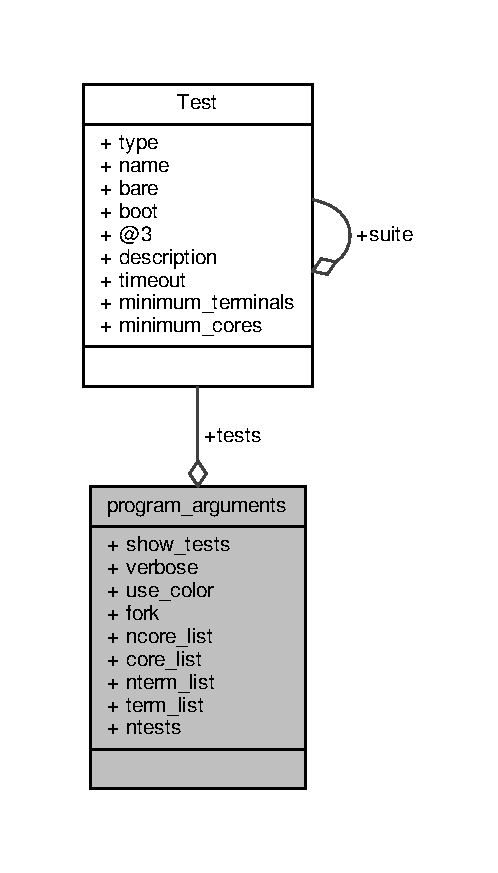
\includegraphics[width=239pt]{structprogram__arguments__coll__graph}
\end{center}
\end{figure}
\subsection*{Data Fields}
\begin{DoxyCompactItemize}
\item 
int \hyperlink{structprogram__arguments_a373cc9d546fdd5ca2c75e42300caf2e6}{show\+\_\+tests}\hypertarget{structprogram__arguments_a373cc9d546fdd5ca2c75e42300caf2e6}{}\label{structprogram__arguments_a373cc9d546fdd5ca2c75e42300caf2e6}

\begin{DoxyCompactList}\small\item\em Flag that we just print the available tests. \end{DoxyCompactList}\item 
int \hyperlink{structprogram__arguments_ab075ba9c1c9d3b650c7490717ed6391e}{verbose}\hypertarget{structprogram__arguments_ab075ba9c1c9d3b650c7490717ed6391e}{}\label{structprogram__arguments_ab075ba9c1c9d3b650c7490717ed6391e}

\begin{DoxyCompactList}\small\item\em Flag verbose. \end{DoxyCompactList}\item 
int \hyperlink{structprogram__arguments_ae952a1ee415137013201280b500796c7}{use\+\_\+color}\hypertarget{structprogram__arguments_ae952a1ee415137013201280b500796c7}{}\label{structprogram__arguments_ae952a1ee415137013201280b500796c7}

\begin{DoxyCompactList}\small\item\em Flag use\+\_\+color. \end{DoxyCompactList}\item 
int \hyperlink{structprogram__arguments_ac8d013f1348ee6c7287fd974561b4f47}{fork}\hypertarget{structprogram__arguments_ac8d013f1348ee6c7287fd974561b4f47}{}\label{structprogram__arguments_ac8d013f1348ee6c7287fd974561b4f47}

\begin{DoxyCompactList}\small\item\em Flag to signal fork. \end{DoxyCompactList}\item 
int \hyperlink{structprogram__arguments_ab9717e16b92f14aa8c54dbf4a2d2b7b1}{ncore\+\_\+list}
\item 
int \hyperlink{structprogram__arguments_ad063b1ce13702392eb2a64792488d505}{core\+\_\+list} \mbox{[}\hyperlink{bios_8h_a009855593b59738d24dbfc236edb3b14}{M\+A\+X\+\_\+\+C\+O\+R\+ES}\mbox{]}\hypertarget{structprogram__arguments_ad063b1ce13702392eb2a64792488d505}{}\label{structprogram__arguments_ad063b1ce13702392eb2a64792488d505}

\begin{DoxyCompactList}\small\item\em List with number of cores. \end{DoxyCompactList}\item 
int \hyperlink{structprogram__arguments_a48fbd16e4ce7ab5438078817c4931108}{nterm\+\_\+list}
\item 
int \hyperlink{structprogram__arguments_ab05abd5478458bb551479eb3e3dc75b1}{term\+\_\+list} \mbox{[}\hyperlink{bios_8h_a4e7d162c7c35103b42768ff4a5c73905}{M\+A\+X\+\_\+\+T\+E\+R\+M\+I\+N\+A\+LS}+1\mbox{]}\hypertarget{structprogram__arguments_ab05abd5478458bb551479eb3e3dc75b1}{}\label{structprogram__arguments_ab05abd5478458bb551479eb3e3dc75b1}

\begin{DoxyCompactList}\small\item\em List with number of terminals. \end{DoxyCompactList}\item 
int \hyperlink{structprogram__arguments_a8b96bf14afced6bae0d45424ab2fac57}{ntests}
\item 
const struct \hyperlink{structTest}{Test} $\ast$ \hyperlink{structprogram__arguments_a1db9e2ccc5b4309d559617d2b327e527}{tests} \mbox{[}\hyperlink{group__Testing_ga2a77d2f2c5b698c69c19e1f8782bf709}{M\+A\+X\+\_\+\+T\+E\+S\+TS}\mbox{]}\hypertarget{structprogram__arguments_a1db9e2ccc5b4309d559617d2b327e527}{}\label{structprogram__arguments_a1db9e2ccc5b4309d559617d2b327e527}

\begin{DoxyCompactList}\small\item\em Tests to run. \end{DoxyCompactList}\end{DoxyCompactItemize}


\subsection{Detailed Description}
Global arguments for test execution. 

Definition at line 208 of file unit\+\_\+testing.\+h.



\subsection{Field Documentation}
\index{program\+\_\+arguments@{program\+\_\+arguments}!ncore\+\_\+list@{ncore\+\_\+list}}
\index{ncore\+\_\+list@{ncore\+\_\+list}!program\+\_\+arguments@{program\+\_\+arguments}}
\subsubsection[{\texorpdfstring{ncore\+\_\+list}{ncore_list}}]{\setlength{\rightskip}{0pt plus 5cm}int program\+\_\+arguments\+::ncore\+\_\+list}\hypertarget{structprogram__arguments_ab9717e16b92f14aa8c54dbf4a2d2b7b1}{}\label{structprogram__arguments_ab9717e16b92f14aa8c54dbf4a2d2b7b1}
Size of {\ttfamily core\+\_\+list} 

Definition at line 223 of file unit\+\_\+testing.\+h.

\index{program\+\_\+arguments@{program\+\_\+arguments}!nterm\+\_\+list@{nterm\+\_\+list}}
\index{nterm\+\_\+list@{nterm\+\_\+list}!program\+\_\+arguments@{program\+\_\+arguments}}
\subsubsection[{\texorpdfstring{nterm\+\_\+list}{nterm_list}}]{\setlength{\rightskip}{0pt plus 5cm}int program\+\_\+arguments\+::nterm\+\_\+list}\hypertarget{structprogram__arguments_a48fbd16e4ce7ab5438078817c4931108}{}\label{structprogram__arguments_a48fbd16e4ce7ab5438078817c4931108}
Size of {\ttfamily term\+\_\+list} 

Definition at line 227 of file unit\+\_\+testing.\+h.

\index{program\+\_\+arguments@{program\+\_\+arguments}!ntests@{ntests}}
\index{ntests@{ntests}!program\+\_\+arguments@{program\+\_\+arguments}}
\subsubsection[{\texorpdfstring{ntests}{ntests}}]{\setlength{\rightskip}{0pt plus 5cm}int program\+\_\+arguments\+::ntests}\hypertarget{structprogram__arguments_a8b96bf14afced6bae0d45424ab2fac57}{}\label{structprogram__arguments_a8b96bf14afced6bae0d45424ab2fac57}
Size of {\ttfamily tests} 

Definition at line 231 of file unit\+\_\+testing.\+h.



The documentation for this struct was generated from the following file\+:\begin{DoxyCompactItemize}
\item 
\hyperlink{unit__testing_8h}{unit\+\_\+testing.\+h}\end{DoxyCompactItemize}

\hypertarget{structresource__list__node}{}\section{resource\+\_\+list\+\_\+node Struct Reference}
\label{structresource__list__node}\index{resource\+\_\+list\+\_\+node@{resource\+\_\+list\+\_\+node}}


List node.  




{\ttfamily \#include $<$util.\+h$>$}



Collaboration diagram for resource\+\_\+list\+\_\+node\+:
\nopagebreak
\begin{figure}[H]
\begin{center}
\leavevmode
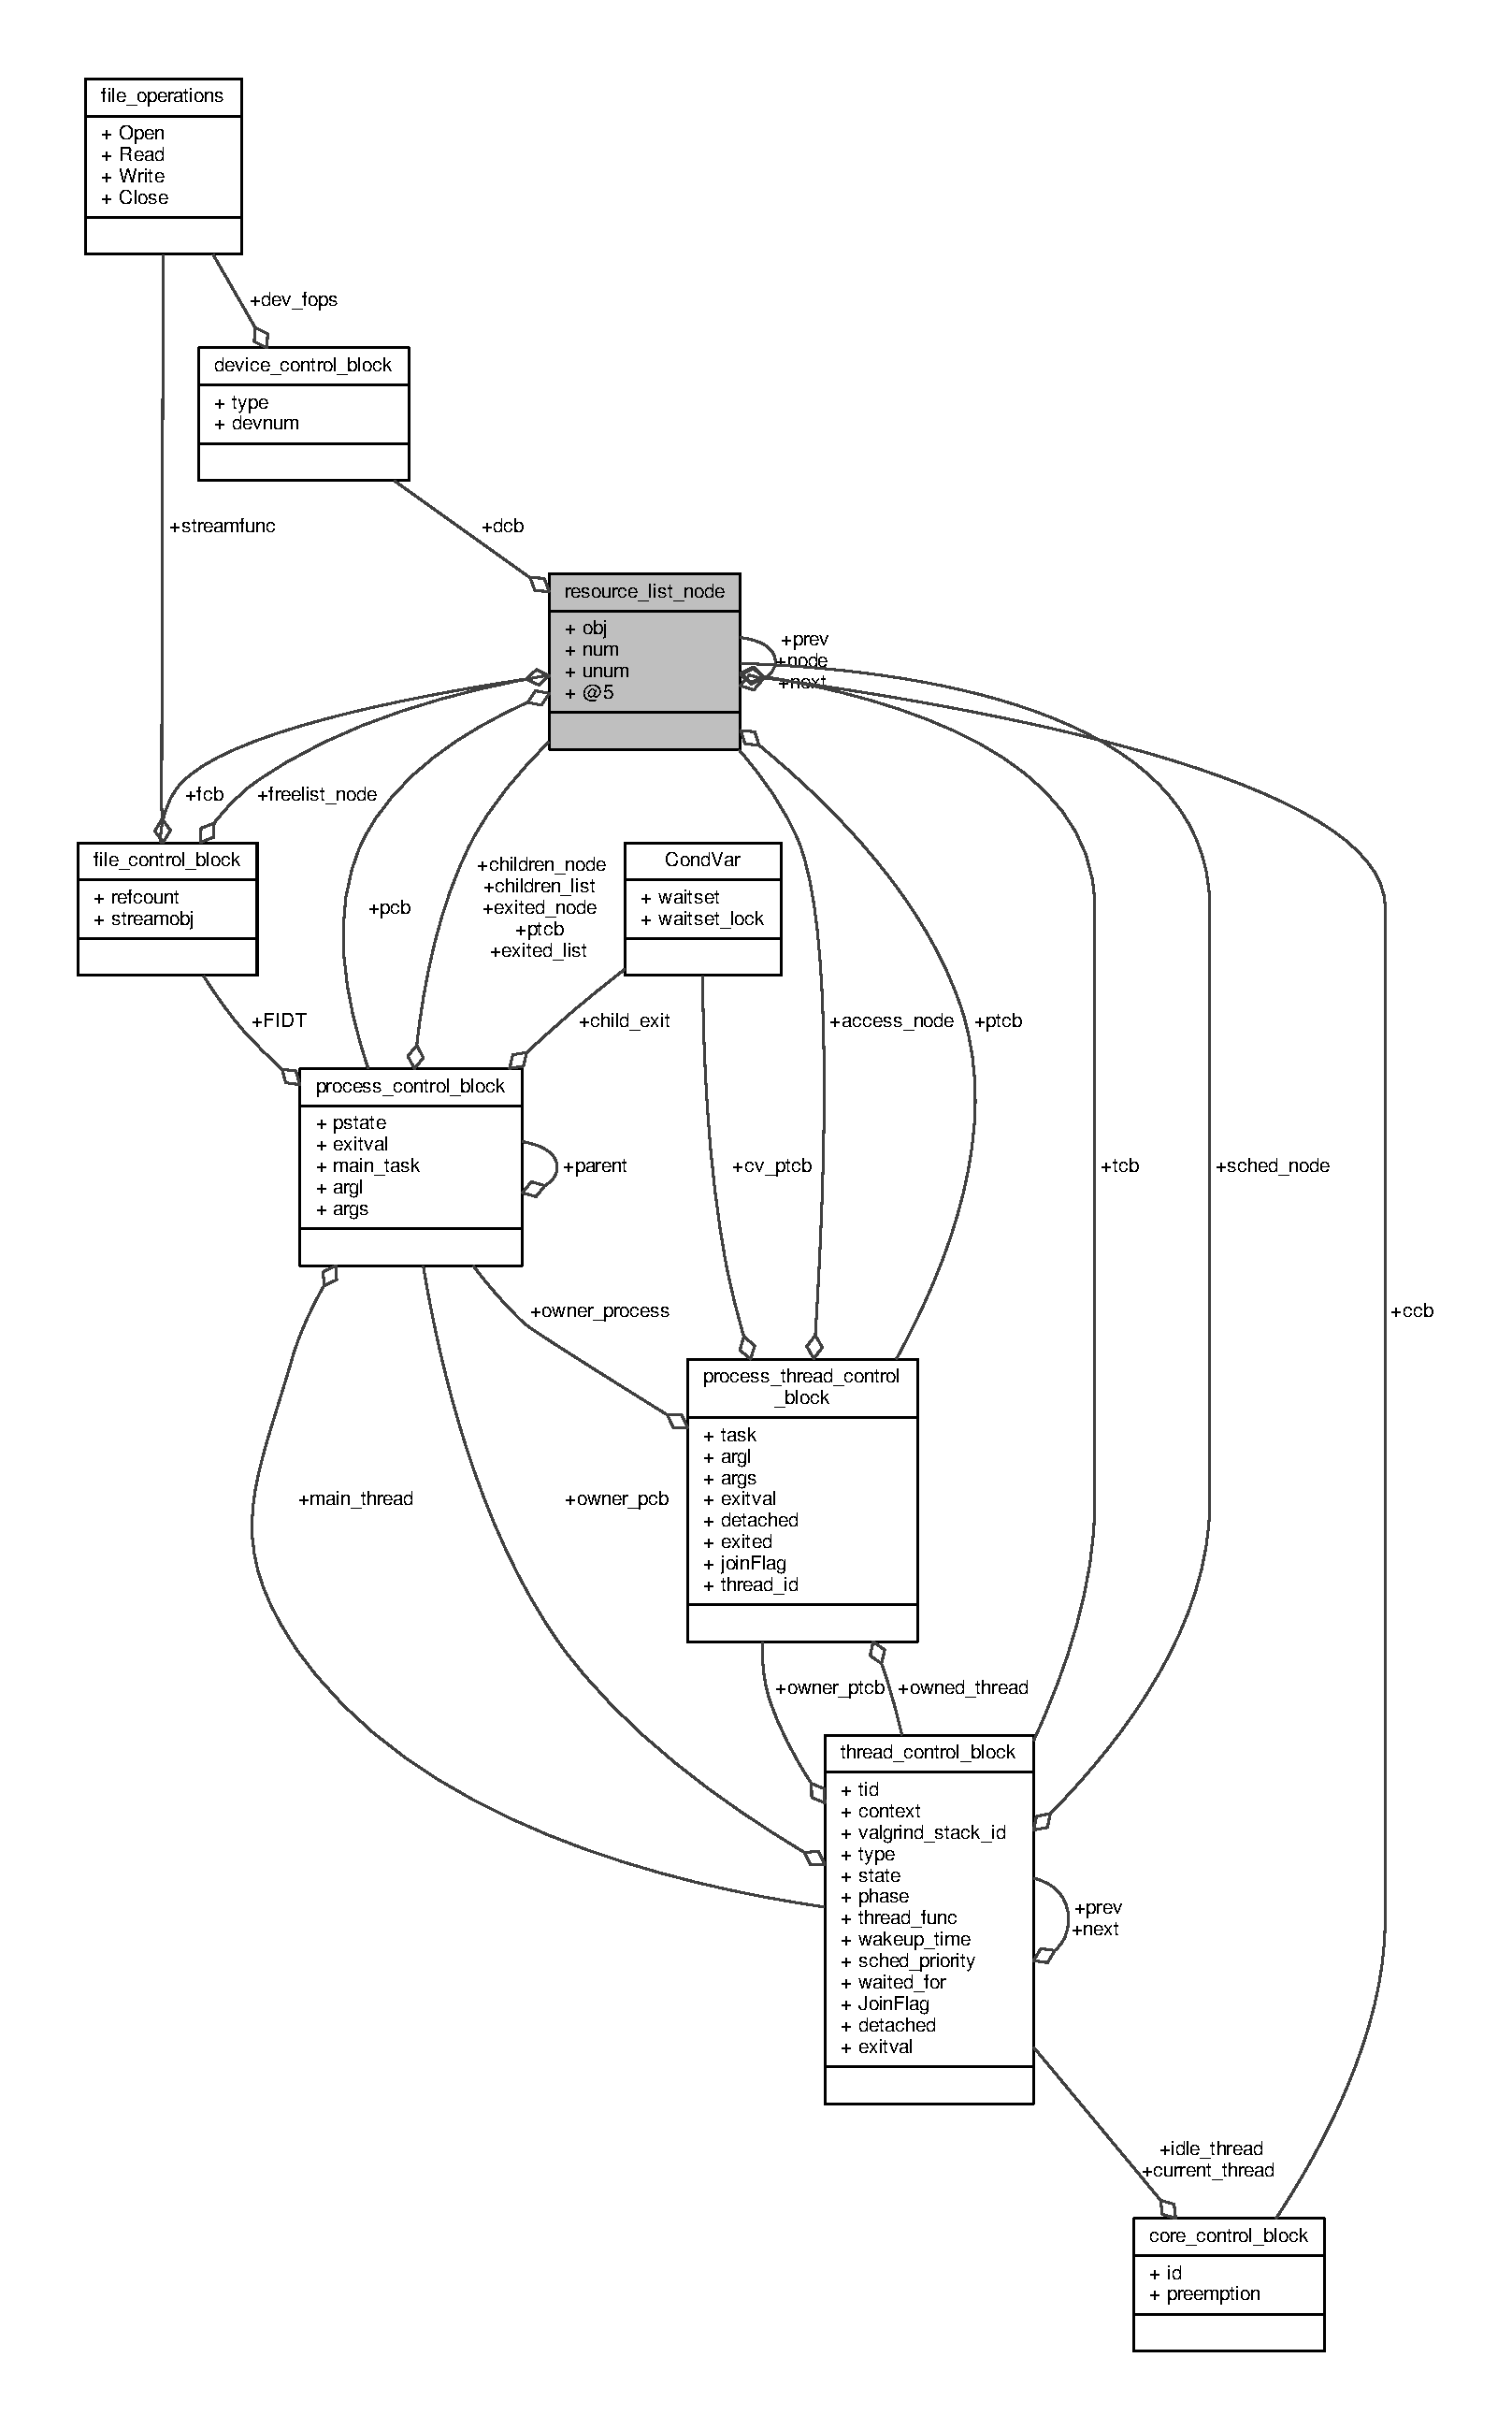
\includegraphics[height=550pt]{structresource__list__node__coll__graph}
\end{center}
\end{figure}
\subsection*{Data Fields}
\begin{DoxyCompactItemize}
\item 
\begin{tabbing}
xx\=xx\=xx\=xx\=xx\=xx\=xx\=xx\=xx\=\kill
union \{\\
\>\hyperlink{structprocess__thread__control__block}{PTCB} $\ast$ {\bfseries ptcb}\\
\>\hyperlink{group__proc_ga91aaadf0c3f9cef2293a99c69795323f}{PCB} $\ast$ {\bfseries pcb}\\
\>\hyperlink{group__scheduler_gaf88d9c946bf70b36a1e8bc34383abfc9}{TCB} $\ast$ {\bfseries tcb}\\
\>\hyperlink{group__scheduler_ga7485b31e0dd9fd723bc2d75fba5206a0}{CCB} $\ast$ {\bfseries ccb}\\
\>\hyperlink{group__dev_gaf0e2d4a982667466d84f6fb7522611d6}{DCB} $\ast$ {\bfseries dcb}\\
\>\hyperlink{group__streams_ga0c7e751afb9d6cadebf070961804d400}{FCB} $\ast$ {\bfseries fcb}\\
\>void $\ast$ {\bfseries obj}\\
\>\hyperlink{group__rlists_gaae2ea9be18d20f0c80a62a2f8e2eed4d}{rlnode\_ptr} {\bfseries node}\\
\>intptr\_t {\bfseries num}\\
\>uintptr\_t {\bfseries unum}\\
\}; \\

\end{tabbing}\begin{DoxyCompactList}\small\item\em The list node\textquotesingle{}s key. \end{DoxyCompactList}\item 
\hyperlink{group__rlists_gaae2ea9be18d20f0c80a62a2f8e2eed4d}{rlnode\+\_\+ptr} \hyperlink{structresource__list__node_a280b77fdcee186bcaade02f76322d183}{prev}\hypertarget{structresource__list__node_a280b77fdcee186bcaade02f76322d183}{}\label{structresource__list__node_a280b77fdcee186bcaade02f76322d183}

\begin{DoxyCompactList}\small\item\em Pointer to previous node. \end{DoxyCompactList}\item 
\hyperlink{group__rlists_gaae2ea9be18d20f0c80a62a2f8e2eed4d}{rlnode\+\_\+ptr} \hyperlink{structresource__list__node_a04b1ee9524cd800f14de2925141e3762}{next}\hypertarget{structresource__list__node_a04b1ee9524cd800f14de2925141e3762}{}\label{structresource__list__node_a04b1ee9524cd800f14de2925141e3762}

\begin{DoxyCompactList}\small\item\em Pointer to next node. \end{DoxyCompactList}\end{DoxyCompactItemize}


\subsection{Detailed Description}
List node. 

Definition at line 300 of file util.\+h.



\subsection{Field Documentation}
\subsubsection[{\texorpdfstring{"@5}{@5}}]{\setlength{\rightskip}{0pt plus 5cm}union \{ ... \} }\hypertarget{structresource__list__node_aba8874eccf1ac3e7657c726a4f86536c}{}\label{structresource__list__node_aba8874eccf1ac3e7657c726a4f86536c}


The list node\textquotesingle{}s key. 

The key (data element) of a list node is stored in a union of several pointer and integer types. This allows for easy access, without the need for casting. For example, 
\begin{DoxyCode}
\hyperlink{structthread__control__block}{TCB}* tcb = mynode->tcb;
\end{DoxyCode}
 

The documentation for this struct was generated from the following file\+:\begin{DoxyCompactItemize}
\item 
\hyperlink{util_8h}{util.\+h}\end{DoxyCompactItemize}

\hypertarget{structserial__device__control__block}{}\section{serial\+\_\+device\+\_\+control\+\_\+block Struct Reference}
\label{structserial__device__control__block}\index{serial\+\_\+device\+\_\+control\+\_\+block@{serial\+\_\+device\+\_\+control\+\_\+block}}


Collaboration diagram for serial\+\_\+device\+\_\+control\+\_\+block\+:\nopagebreak
\begin{figure}[H]
\begin{center}
\leavevmode
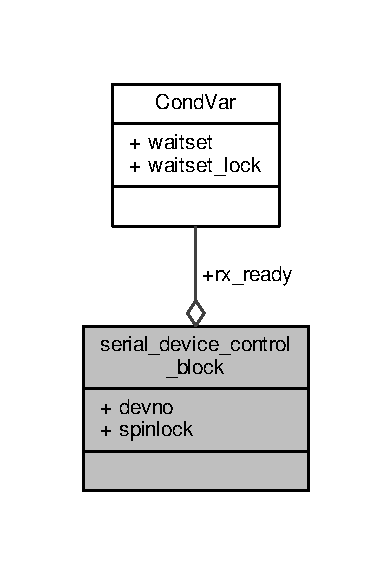
\includegraphics[width=188pt]{structserial__device__control__block__coll__graph}
\end{center}
\end{figure}
\subsection*{Data Fields}
\begin{DoxyCompactItemize}
\item 
\hyperlink{bios_8h_a91ad9478d81a7aaf2593e8d9c3d06a14}{uint} {\bfseries devno}\hypertarget{structserial__device__control__block_a44ef944c9ed235eff02cba42f44487c6}{}\label{structserial__device__control__block_a44ef944c9ed235eff02cba42f44487c6}

\item 
\hyperlink{group__syscalls_gaef2ec62cae8e0031fd19fc8b91083ade}{Mutex} {\bfseries spinlock}\hypertarget{structserial__device__control__block_a8861a6dc00a780bf5641f6945bf276cc}{}\label{structserial__device__control__block_a8861a6dc00a780bf5641f6945bf276cc}

\item 
\hyperlink{structCondVar}{Cond\+Var} {\bfseries rx\+\_\+ready}\hypertarget{structserial__device__control__block_a2b0916cc5b259d64ebe85743ab89b84e}{}\label{structserial__device__control__block_a2b0916cc5b259d64ebe85743ab89b84e}

\end{DoxyCompactItemize}


\subsection{Detailed Description}


Definition at line 69 of file kernel\+\_\+dev.\+c.



The documentation for this struct was generated from the following file\+:\begin{DoxyCompactItemize}
\item 
kernel\+\_\+dev.\+c\end{DoxyCompactItemize}

\hypertarget{structsocket__control__block}{}\section{socket\+\_\+control\+\_\+block Struct Reference}
\label{structsocket__control__block}\index{socket\+\_\+control\+\_\+block@{socket\+\_\+control\+\_\+block}}


Collaboration diagram for socket\+\_\+control\+\_\+block\+:
\nopagebreak
\begin{figure}[H]
\begin{center}
\leavevmode
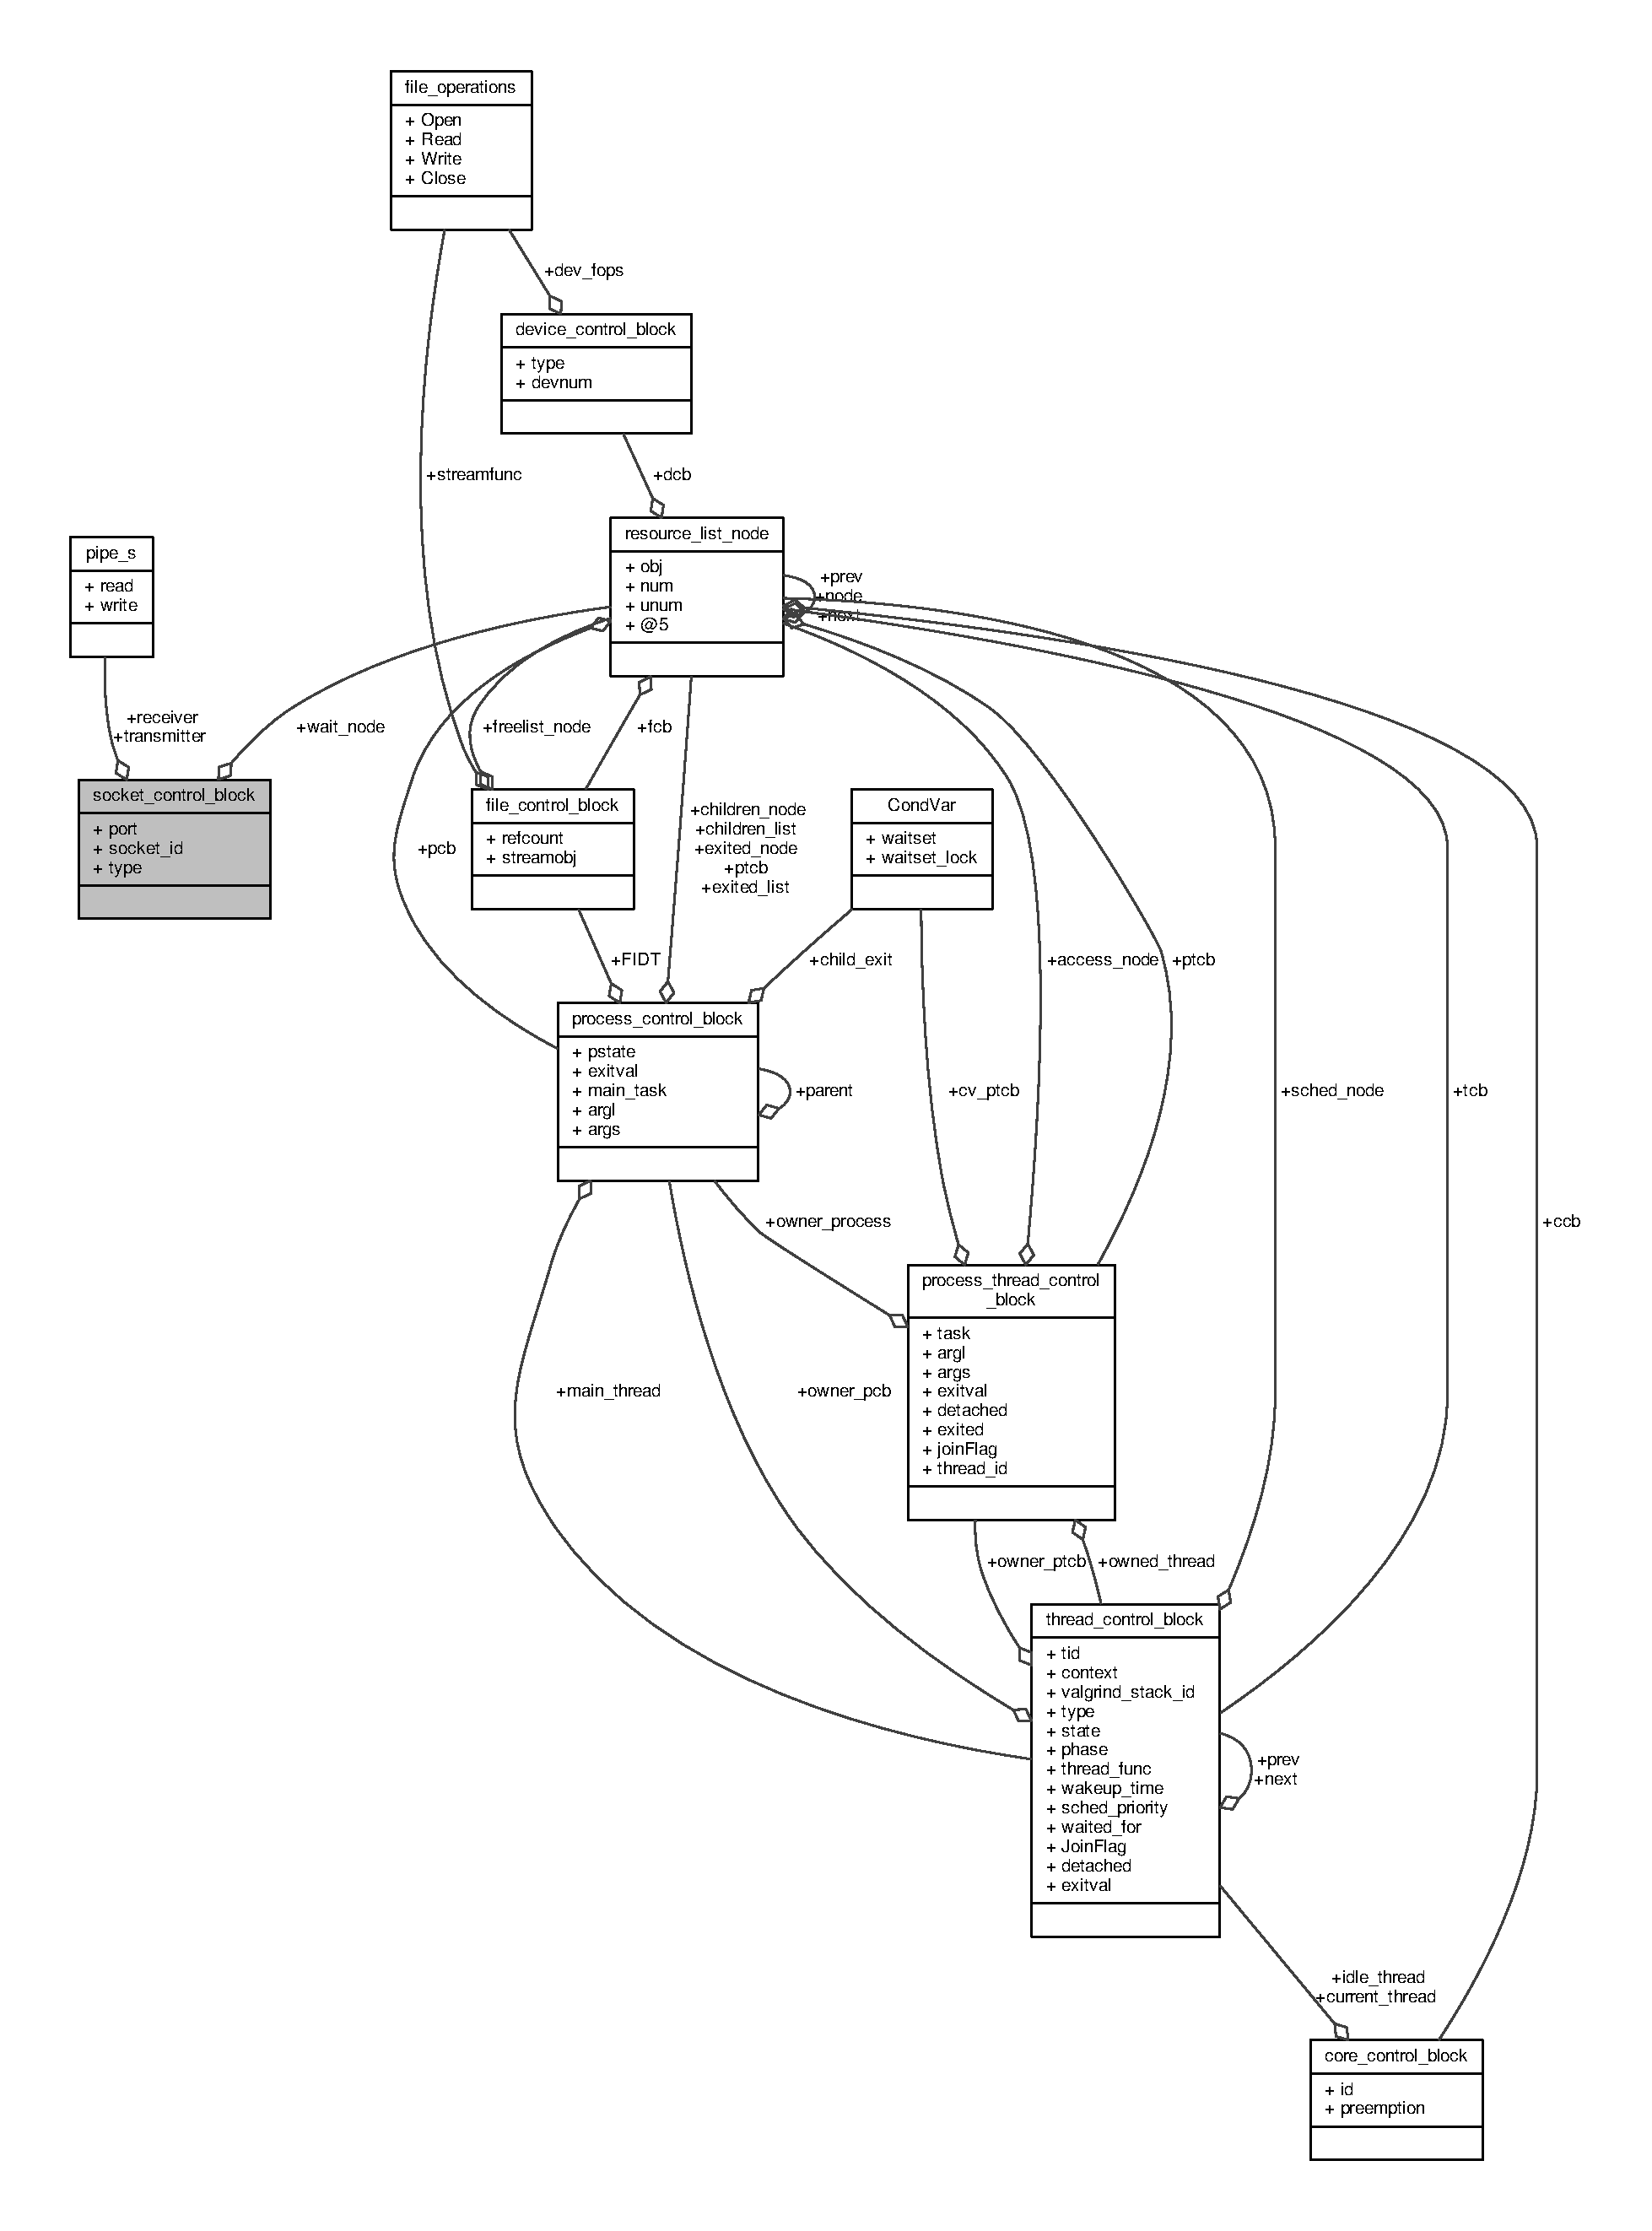
\includegraphics[width=350pt]{structsocket__control__block__coll__graph}
\end{center}
\end{figure}
\subsection*{Data Fields}
\begin{DoxyCompactItemize}
\item 
\hyperlink{group__syscalls_ga13894e5a2ffd5febb7aeb90e87239d61}{port\+\_\+t} {\bfseries port}\hypertarget{structsocket__control__block_a423683847ce85a4d78ea2830e3eb938d}{}\label{structsocket__control__block_a423683847ce85a4d78ea2830e3eb938d}

\item 
\hyperlink{group__syscalls_gad56b5ceaaf7d3ab88b4be7f622314dfb}{pipe\+\_\+t} {\bfseries transmitter}\hypertarget{structsocket__control__block_ac170296c34ccae8e6898c414ebc2bf16}{}\label{structsocket__control__block_ac170296c34ccae8e6898c414ebc2bf16}

\item 
\hyperlink{group__syscalls_gad56b5ceaaf7d3ab88b4be7f622314dfb}{pipe\+\_\+t} {\bfseries receiver}\hypertarget{structsocket__control__block_a391aacf4e12a923f9b284829b60e44b8}{}\label{structsocket__control__block_a391aacf4e12a923f9b284829b60e44b8}

\item 
\hyperlink{group__rlists_ga8f6244877f7ce2322c90525217ea6e7a}{rlnode} {\bfseries wait\+\_\+node}\hypertarget{structsocket__control__block_a9f64ee3e191c8072eddddeb2ed4ed06a}{}\label{structsocket__control__block_a9f64ee3e191c8072eddddeb2ed4ed06a}

\item 
\hyperlink{group__syscalls_ga5097222c5f0da97d92d4712359abc38f}{Fid\+\_\+t} {\bfseries socket\+\_\+id}\hypertarget{structsocket__control__block_aa0ca17a7e9a5f8994e85a4fe8b6818b7}{}\label{structsocket__control__block_aa0ca17a7e9a5f8994e85a4fe8b6818b7}

\item 
socket\+\_\+type {\bfseries type}\hypertarget{structsocket__control__block_aff33160bc35e844f2262cf907a6077de}{}\label{structsocket__control__block_aff33160bc35e844f2262cf907a6077de}

\end{DoxyCompactItemize}


\subsection{Detailed Description}


Definition at line 27 of file kernel\+\_\+socket.\+c.



The documentation for this struct was generated from the following file\+:\begin{DoxyCompactItemize}
\item 
kernel\+\_\+socket.\+c\end{DoxyCompactItemize}

\hypertarget{structsymposium__t}{}\section{symposium\+\_\+t Struct Reference}
\label{structsymposium__t}\index{symposium\+\_\+t@{symposium\+\_\+t}}


A symposium definition.  




{\ttfamily \#include $<$symposium.\+h$>$}



Collaboration diagram for symposium\+\_\+t\+:\nopagebreak
\begin{figure}[H]
\begin{center}
\leavevmode
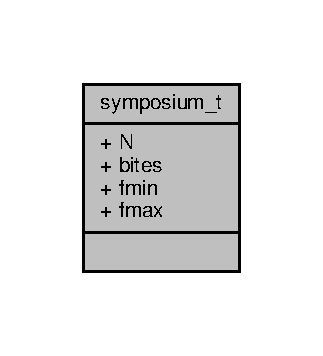
\includegraphics[width=155pt]{structsymposium__t__coll__graph}
\end{center}
\end{figure}
\subsection*{Data Fields}
\begin{DoxyCompactItemize}
\item 
int \hyperlink{structsymposium__t_a4e366c10036b2d89ebc2dbcdefba8999}{N}
\item 
int \hyperlink{structsymposium__t_a9ee1b978200b8a4b7c30b170c1f20643}{bites}
\item 
int {\bfseries fmin}\hypertarget{structsymposium__t_ab7af5af3a92d6c03bf916571a09d6aed}{}\label{structsymposium__t_ab7af5af3a92d6c03bf916571a09d6aed}

\item 
int \hyperlink{structsymposium__t_a038b49a350225fed31d5c148a9147ec6}{fmax}
\end{DoxyCompactItemize}


\subsection{Detailed Description}
A symposium definition. 

The four numbers defining a symposium. 

Definition at line 82 of file symposium.\+h.



\subsection{Field Documentation}
\index{symposium\+\_\+t@{symposium\+\_\+t}!bites@{bites}}
\index{bites@{bites}!symposium\+\_\+t@{symposium\+\_\+t}}
\subsubsection[{\texorpdfstring{bites}{bites}}]{\setlength{\rightskip}{0pt plus 5cm}int symposium\+\_\+t\+::bites}\hypertarget{structsymposium__t_a9ee1b978200b8a4b7c30b170c1f20643}{}\label{structsymposium__t_a9ee1b978200b8a4b7c30b170c1f20643}
Number of bites each philosopher takes. 

Definition at line 84 of file symposium.\+h.

\index{symposium\+\_\+t@{symposium\+\_\+t}!fmax@{fmax}}
\index{fmax@{fmax}!symposium\+\_\+t@{symposium\+\_\+t}}
\subsubsection[{\texorpdfstring{fmax}{fmax}}]{\setlength{\rightskip}{0pt plus 5cm}int symposium\+\_\+t\+::fmax}\hypertarget{structsymposium__t_a038b49a350225fed31d5c148a9147ec6}{}\label{structsymposium__t_a038b49a350225fed31d5c148a9147ec6}
Values used by the Fibbonacci routines 

Definition at line 85 of file symposium.\+h.

\index{symposium\+\_\+t@{symposium\+\_\+t}!N@{N}}
\index{N@{N}!symposium\+\_\+t@{symposium\+\_\+t}}
\subsubsection[{\texorpdfstring{N}{N}}]{\setlength{\rightskip}{0pt plus 5cm}int symposium\+\_\+t\+::N}\hypertarget{structsymposium__t_a4e366c10036b2d89ebc2dbcdefba8999}{}\label{structsymposium__t_a4e366c10036b2d89ebc2dbcdefba8999}
Number of philosophers 

Definition at line 83 of file symposium.\+h.



The documentation for this struct was generated from the following file\+:\begin{DoxyCompactItemize}
\item 
\hyperlink{symposium_8h}{symposium.\+h}\end{DoxyCompactItemize}

\hypertarget{structSymposiumTable}{}\section{Symposium\+Table Struct Reference}
\label{structSymposiumTable}\index{Symposium\+Table@{Symposium\+Table}}


A symposium monitor.  




{\ttfamily \#include $<$symposium.\+h$>$}



Collaboration diagram for Symposium\+Table\+:\nopagebreak
\begin{figure}[H]
\begin{center}
\leavevmode
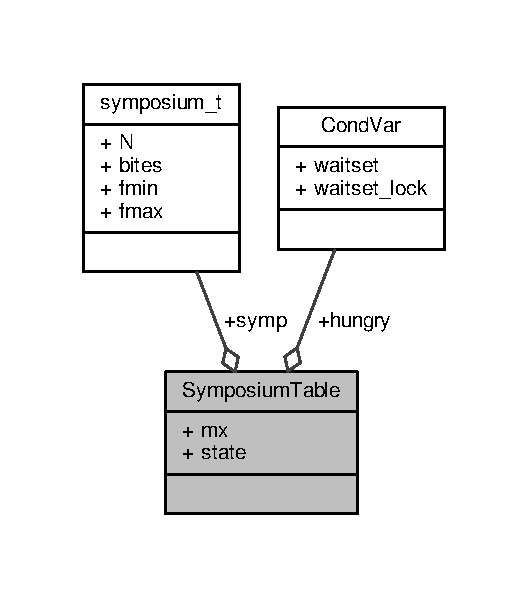
\includegraphics[width=254pt]{structSymposiumTable__coll__graph}
\end{center}
\end{figure}
\subsection*{Data Fields}
\begin{DoxyCompactItemize}
\item 
\hyperlink{group__syscalls_gaef2ec62cae8e0031fd19fc8b91083ade}{Mutex} \hyperlink{structSymposiumTable_a8c36f26f523e6b2f99f6e70fff098de8}{mx}
\item 
\hyperlink{structsymposium__t}{symposium\+\_\+t} $\ast$ \hyperlink{structSymposiumTable_a4089e2778ba23eb79c4785eb5702f70f}{symp}
\item 
\hyperlink{symposium_8h_a9fced5fb7d50a8fa2e8ae45b0cae3520}{P\+H\+IL} $\ast$ \hyperlink{structSymposiumTable_a70507f28df670d0db2e59fc65309af08}{state}
\item 
\hyperlink{structCondVar}{Cond\+Var} $\ast$ \hyperlink{structSymposiumTable_a6daa1fdbfe8e836e72bfd6953bc91f6e}{hungry}
\end{DoxyCompactItemize}


\subsection{Detailed Description}
A symposium monitor. 

Such an object must be shared between all philosopher threads/processes. 

Definition at line 113 of file symposium.\+h.



\subsection{Field Documentation}
\index{Symposium\+Table@{Symposium\+Table}!hungry@{hungry}}
\index{hungry@{hungry}!Symposium\+Table@{Symposium\+Table}}
\subsubsection[{\texorpdfstring{hungry}{hungry}}]{\setlength{\rightskip}{0pt plus 5cm}{\bf Cond\+Var}$\ast$ Symposium\+Table\+::hungry}\hypertarget{structSymposiumTable_a6daa1fdbfe8e836e72bfd6953bc91f6e}{}\label{structSymposiumTable_a6daa1fdbfe8e836e72bfd6953bc91f6e}
hungry\mbox{[}i\mbox{]} i=...N\+: condition var for philosophers 

Definition at line 117 of file symposium.\+h.

\index{Symposium\+Table@{Symposium\+Table}!mx@{mx}}
\index{mx@{mx}!Symposium\+Table@{Symposium\+Table}}
\subsubsection[{\texorpdfstring{mx}{mx}}]{\setlength{\rightskip}{0pt plus 5cm}{\bf Mutex} Symposium\+Table\+::mx}\hypertarget{structSymposiumTable_a8c36f26f523e6b2f99f6e70fff098de8}{}\label{structSymposiumTable_a8c36f26f523e6b2f99f6e70fff098de8}
Monitor mutex 

Definition at line 114 of file symposium.\+h.

\index{Symposium\+Table@{Symposium\+Table}!state@{state}}
\index{state@{state}!Symposium\+Table@{Symposium\+Table}}
\subsubsection[{\texorpdfstring{state}{state}}]{\setlength{\rightskip}{0pt plus 5cm}{\bf P\+H\+IL}$\ast$ Symposium\+Table\+::state}\hypertarget{structSymposiumTable_a70507f28df670d0db2e59fc65309af08}{}\label{structSymposiumTable_a70507f28df670d0db2e59fc65309af08}
state\mbox{[}i\mbox{]} i=1...N\mbox{]}\+: Philosopher state 

Definition at line 116 of file symposium.\+h.

\index{Symposium\+Table@{Symposium\+Table}!symp@{symp}}
\index{symp@{symp}!Symposium\+Table@{Symposium\+Table}}
\subsubsection[{\texorpdfstring{symp}{symp}}]{\setlength{\rightskip}{0pt plus 5cm}{\bf symposium\+\_\+t}$\ast$ Symposium\+Table\+::symp}\hypertarget{structSymposiumTable_a4089e2778ba23eb79c4785eb5702f70f}{}\label{structSymposiumTable_a4089e2778ba23eb79c4785eb5702f70f}
The symposium definition 

Definition at line 115 of file symposium.\+h.



The documentation for this struct was generated from the following file\+:\begin{DoxyCompactItemize}
\item 
\hyperlink{symposium_8h}{symposium.\+h}\end{DoxyCompactItemize}

\hypertarget{structTest}{}\section{Test Struct Reference}
\label{structTest}\index{Test@{Test}}


\hyperlink{structTest}{Test} descriptor.  




{\ttfamily \#include $<$unit\+\_\+testing.\+h$>$}



Collaboration diagram for Test\+:
\nopagebreak
\begin{figure}[H]
\begin{center}
\leavevmode
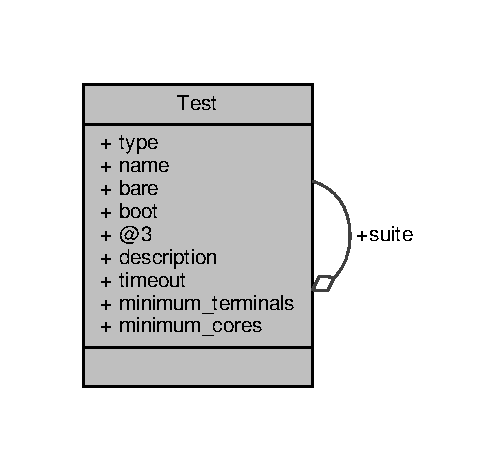
\includegraphics[width=239pt]{structTest__coll__graph}
\end{center}
\end{figure}
\subsection*{Data Fields}
\begin{DoxyCompactItemize}
\item 
Test\+\_\+type \hyperlink{structTest_a5074007b777ea0958966027197c17792}{type}
\item 
const char $\ast$ \hyperlink{structTest_ae44674e48b203d9c26e04e09b6fe5b61}{name}
\item 
\begin{tabbing}
xx\=xx\=xx\=xx\=xx\=xx\=xx\=xx\=xx\=\kill
union \{\\
\>void($\ast$ {\bfseries bare} )(void)\\
\>\hyperlink{group__syscalls_gaec3f2f835e105271fbbc00272c0ba984}{Task} {\bfseries boot}\\
\>const struct \hyperlink{structTest}{Test} $\ast$$\ast$ {\bfseries suite}\\
\}; \\

\end{tabbing}\item 
const char $\ast$ \hyperlink{structTest_a294ca3f1114240c908f66216afcad783}{description}
\item 
unsigned int \hyperlink{structTest_a80e78f2e6aeed2a6e5b7c705ce5a1493}{timeout}
\item 
unsigned int \hyperlink{structTest_a2741188633c51b8e3cb545fa3971bf60}{minimum\+\_\+terminals}
\item 
unsigned int \hyperlink{structTest_ac203918837b4c6718a020246e189a95a}{minimum\+\_\+cores}
\end{DoxyCompactItemize}


\subsection{Detailed Description}
\hyperlink{structTest}{Test} descriptor. 

This object describes a test. 

Definition at line 309 of file unit\+\_\+testing.\+h.



\subsection{Field Documentation}
\subsubsection[{\texorpdfstring{"@3}{@3}}]{\setlength{\rightskip}{0pt plus 5cm}union \{ ... \} }\hypertarget{structTest_a6dd50dae1a4469e7723e85331dbf9ba0}{}\label{structTest_a6dd50dae1a4469e7723e85331dbf9ba0}
\hyperlink{structTest}{Test} function, or list of tests \index{Test@{Test}!description@{description}}
\index{description@{description}!Test@{Test}}
\subsubsection[{\texorpdfstring{description}{description}}]{\setlength{\rightskip}{0pt plus 5cm}const char$\ast$ Test\+::description}\hypertarget{structTest_a294ca3f1114240c908f66216afcad783}{}\label{structTest_a294ca3f1114240c908f66216afcad783}
Human-\/readable, for printing 

Definition at line 318 of file unit\+\_\+testing.\+h.

\index{Test@{Test}!minimum\+\_\+cores@{minimum\+\_\+cores}}
\index{minimum\+\_\+cores@{minimum\+\_\+cores}!Test@{Test}}
\subsubsection[{\texorpdfstring{minimum\+\_\+cores}{minimum_cores}}]{\setlength{\rightskip}{0pt plus 5cm}unsigned int Test\+::minimum\+\_\+cores}\hypertarget{structTest_ac203918837b4c6718a020246e189a95a}{}\label{structTest_ac203918837b4c6718a020246e189a95a}
Minimum no. of cores required. Default\+: 1 

Definition at line 321 of file unit\+\_\+testing.\+h.

\index{Test@{Test}!minimum\+\_\+terminals@{minimum\+\_\+terminals}}
\index{minimum\+\_\+terminals@{minimum\+\_\+terminals}!Test@{Test}}
\subsubsection[{\texorpdfstring{minimum\+\_\+terminals}{minimum_terminals}}]{\setlength{\rightskip}{0pt plus 5cm}unsigned int Test\+::minimum\+\_\+terminals}\hypertarget{structTest_a2741188633c51b8e3cb545fa3971bf60}{}\label{structTest_a2741188633c51b8e3cb545fa3971bf60}
Minimum no. of terminals required. Default\+: 0 

Definition at line 320 of file unit\+\_\+testing.\+h.

\index{Test@{Test}!name@{name}}
\index{name@{name}!Test@{Test}}
\subsubsection[{\texorpdfstring{name}{name}}]{\setlength{\rightskip}{0pt plus 5cm}const char$\ast$ Test\+::name}\hypertarget{structTest_ae44674e48b203d9c26e04e09b6fe5b61}{}\label{structTest_ae44674e48b203d9c26e04e09b6fe5b61}
\hyperlink{structTest}{Test} name 

Definition at line 312 of file unit\+\_\+testing.\+h.

\index{Test@{Test}!timeout@{timeout}}
\index{timeout@{timeout}!Test@{Test}}
\subsubsection[{\texorpdfstring{timeout}{timeout}}]{\setlength{\rightskip}{0pt plus 5cm}unsigned int Test\+::timeout}\hypertarget{structTest_a80e78f2e6aeed2a6e5b7c705ce5a1493}{}\label{structTest_a80e78f2e6aeed2a6e5b7c705ce5a1493}
time to kill test (see D\+E\+F\+A\+U\+L\+T\+\_\+\+T\+I\+M\+E\+O\+UT) 

Definition at line 319 of file unit\+\_\+testing.\+h.

\index{Test@{Test}!type@{type}}
\index{type@{type}!Test@{Test}}
\subsubsection[{\texorpdfstring{type}{type}}]{\setlength{\rightskip}{0pt plus 5cm}Test\+\_\+type Test\+::type}\hypertarget{structTest_a5074007b777ea0958966027197c17792}{}\label{structTest_a5074007b777ea0958966027197c17792}
Bare, boot or suite 

Definition at line 311 of file unit\+\_\+testing.\+h.



The documentation for this struct was generated from the following file\+:\begin{DoxyCompactItemize}
\item 
\hyperlink{unit__testing_8h}{unit\+\_\+testing.\+h}\end{DoxyCompactItemize}

\hypertarget{structthread__control__block}{}\section{thread\+\_\+control\+\_\+block Struct Reference}
\label{structthread__control__block}\index{thread\+\_\+control\+\_\+block@{thread\+\_\+control\+\_\+block}}


The thread control block.  




{\ttfamily \#include $<$kernel\+\_\+sched.\+h$>$}



Collaboration diagram for thread\+\_\+control\+\_\+block\+:
\nopagebreak
\begin{figure}[H]
\begin{center}
\leavevmode
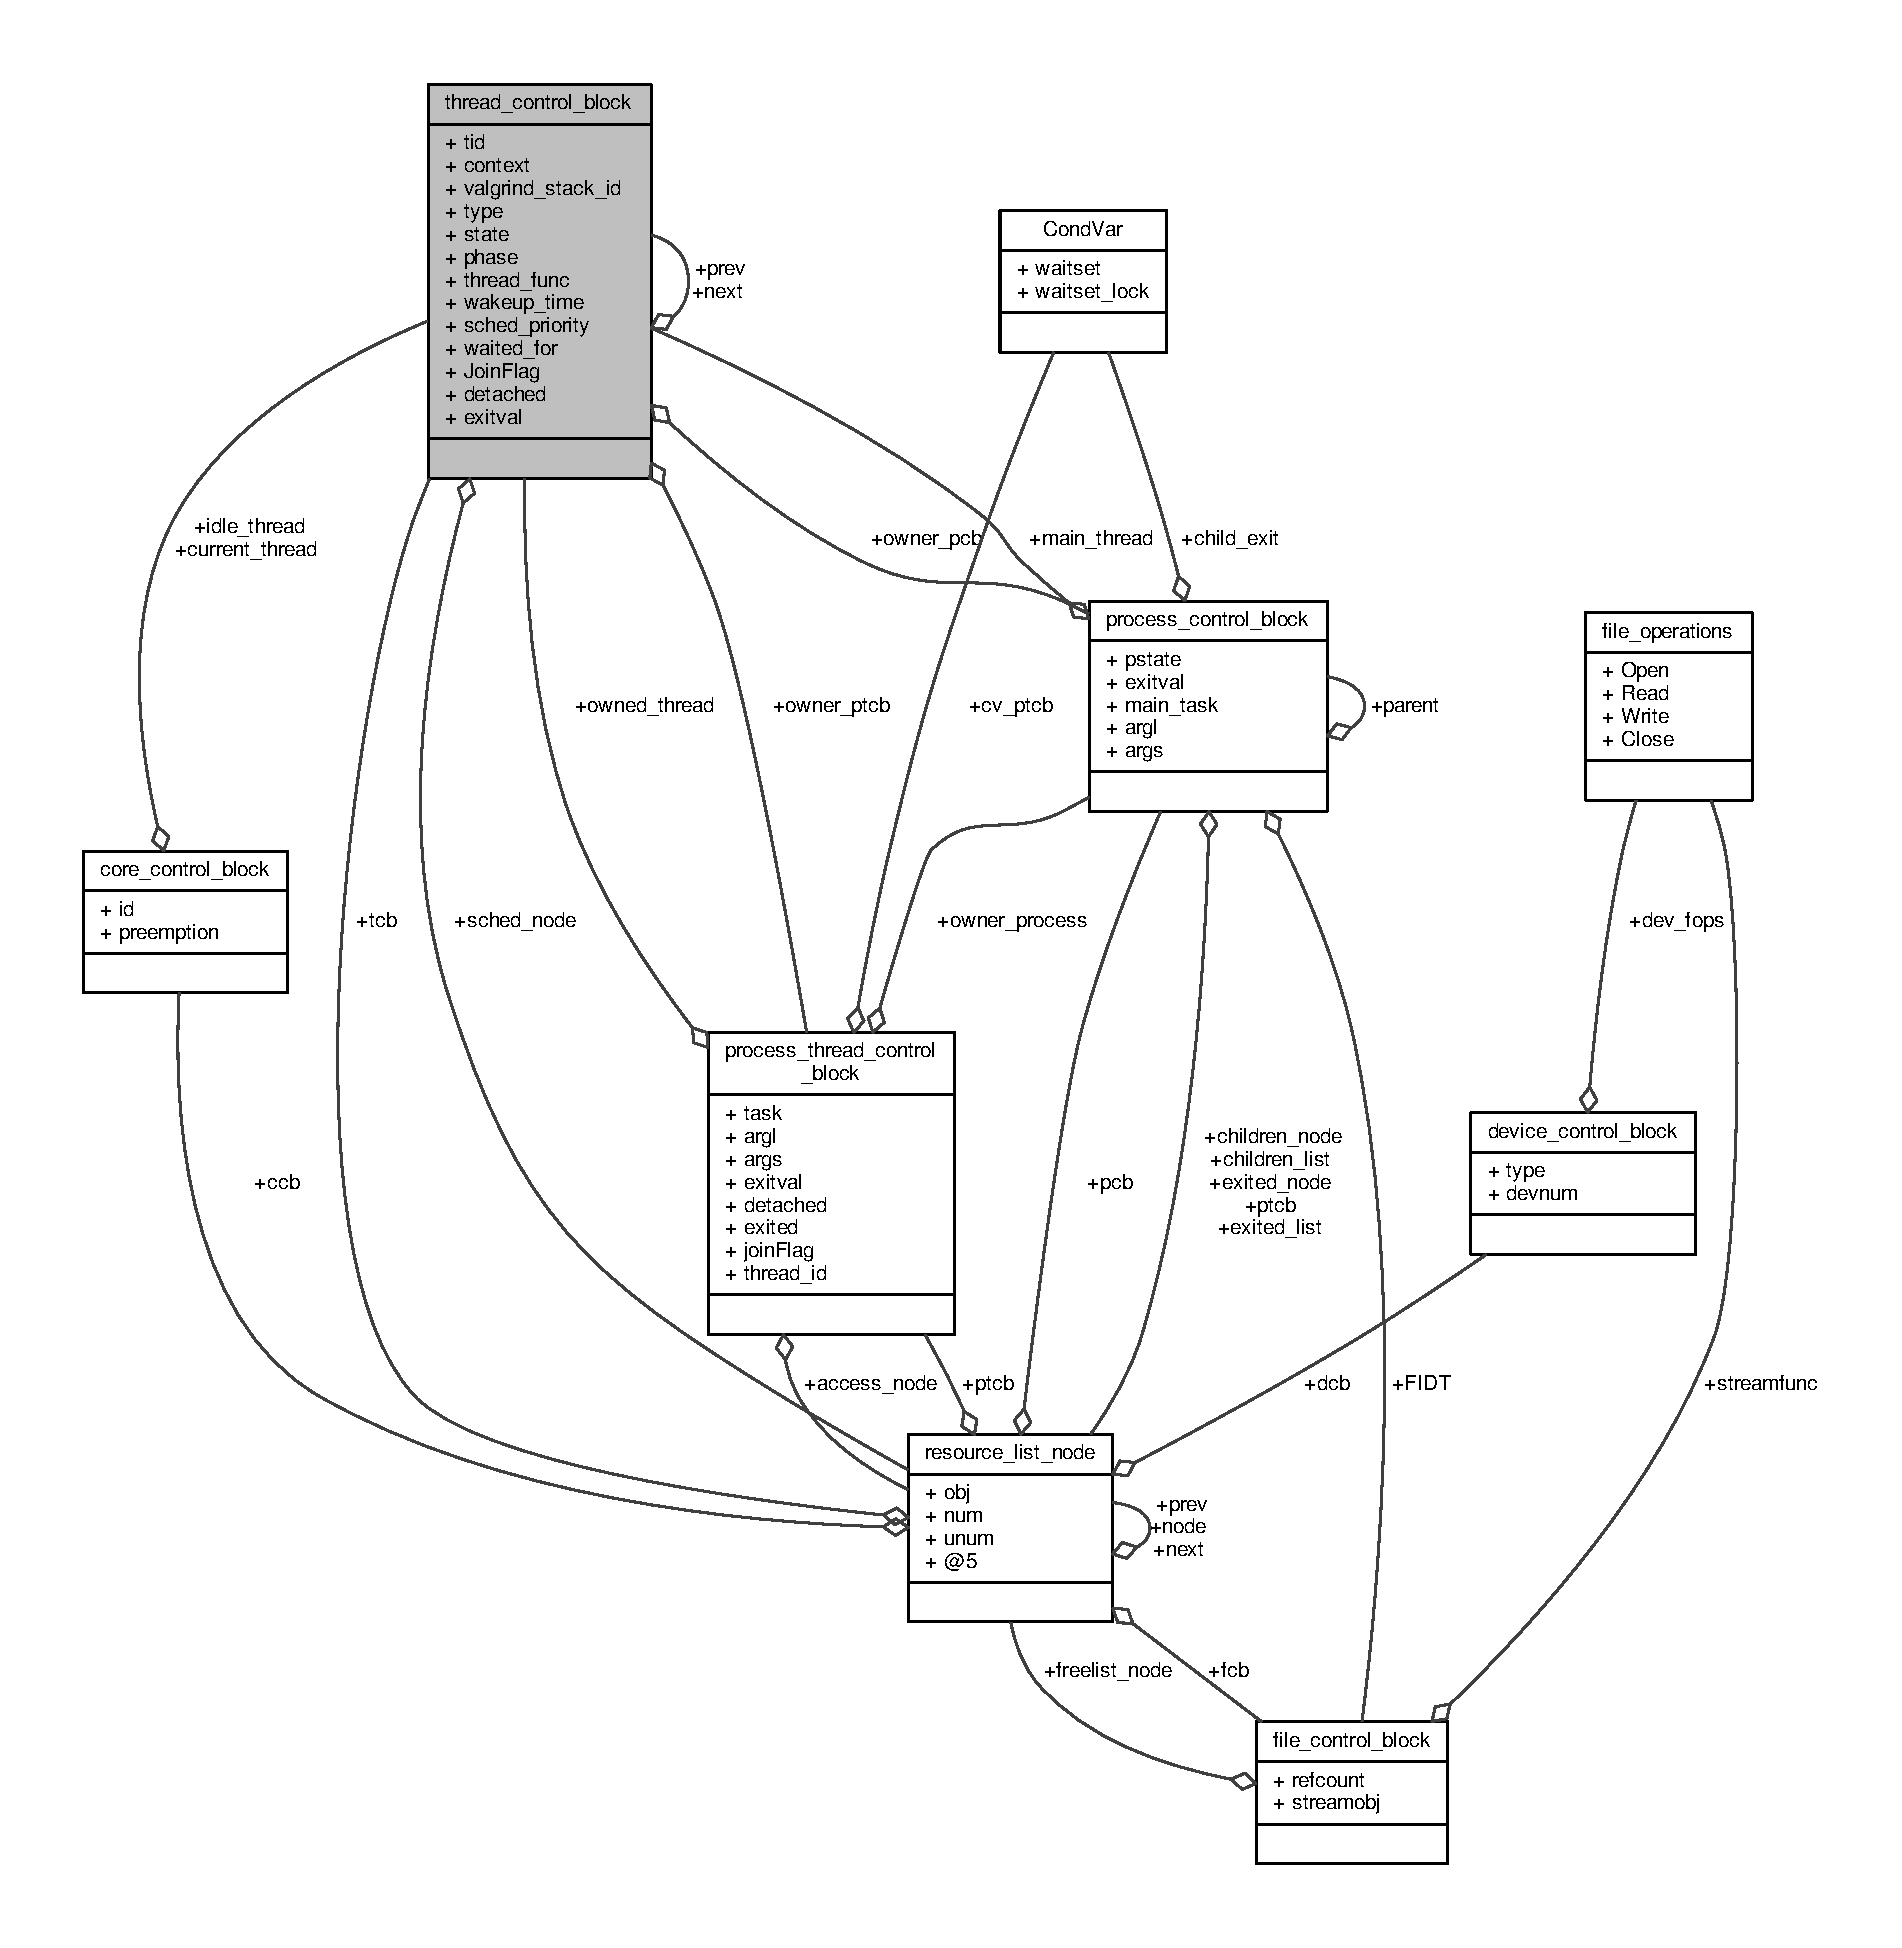
\includegraphics[width=350pt]{structthread__control__block__coll__graph}
\end{center}
\end{figure}
\subsection*{Data Fields}
\begin{DoxyCompactItemize}
\item 
\hyperlink{group__syscalls_gaf67ad1c55e6b2a79bf8a99106380ce01}{Tid\+\_\+t} {\bfseries tid}\hypertarget{structthread__control__block_a76c53858bfcc21ebd103e52255df554b}{}\label{structthread__control__block_a76c53858bfcc21ebd103e52255df554b}

\item 
\hyperlink{group__proc_ga91aaadf0c3f9cef2293a99c69795323f}{P\+CB} $\ast$ \hyperlink{structthread__control__block_a74aa312623cb8be2bc719d5210b58c04}{owner\+\_\+pcb}
\item 
\hyperlink{structprocess__thread__control__block}{P\+T\+CB} $\ast$ {\bfseries owner\+\_\+ptcb}\hypertarget{structthread__control__block_ae9b6a0650c4cf3fd826669ae3da4ef00}{}\label{structthread__control__block_ae9b6a0650c4cf3fd826669ae3da4ef00}

\item 
\hyperlink{bios_8h_a6067c1395a75fc3e17f1ea6353065b54}{cpu\+\_\+context\+\_\+t} \hyperlink{structthread__control__block_a9c107039dffa851dde6edabd6cd3f89c}{context}
\item 
unsigned \hyperlink{structthread__control__block_ad8a2da36c0ad775c12c5f66f4fec9d41}{valgrind\+\_\+stack\+\_\+id}
\item 
\hyperlink{group__scheduler_ga18795bc1ab00161fc27ce34b1895fb03}{Thread\+\_\+type} \hyperlink{structthread__control__block_abd0f40bdcb22c701df03f560bbc42d5c}{type}
\item 
\hyperlink{group__scheduler_ga6c969c169777f82c104cf73e501df70f}{Thread\+\_\+state} \hyperlink{structthread__control__block_affd872365cf4768fa1c9bd1e196bb97c}{state}
\item 
\hyperlink{group__scheduler_gab180b4aa356776bddcd724cef4f5deae}{Thread\+\_\+phase} \hyperlink{structthread__control__block_aa7e8e6a00c5f9f25210a49589ad818f8}{phase}
\item 
void($\ast$ \hyperlink{structthread__control__block_a91a73f2ad3f727b7412b912b3d65109a}{thread\+\_\+func} )()
\item 
\hyperlink{bios_8h_ae7291e5cd742fb9bc6d4aaa0d51bd0ee}{Timer\+Duration} \hyperlink{structthread__control__block_a7dbf9ba7df67911abb7951e249f587b6}{wakeup\+\_\+time}
\item 
\hyperlink{group__rlists_ga8f6244877f7ce2322c90525217ea6e7a}{rlnode} \hyperlink{structthread__control__block_add433b079e04053fe70fdd2b92e1d6ad}{sched\+\_\+node}
\item 
struct \hyperlink{structthread__control__block}{thread\+\_\+control\+\_\+block} $\ast$ \hyperlink{structthread__control__block_a605a6e9bb8154b658ee72e193599d180}{prev}
\item 
struct \hyperlink{structthread__control__block}{thread\+\_\+control\+\_\+block} $\ast$ \hyperlink{structthread__control__block_ac6b51ca735291f730ca1d4c335fb9359}{next}
\item 
int {\bfseries sched\+\_\+priority}\hypertarget{structthread__control__block_aa12eeaf590e1e878b1dd35916958c090}{}\label{structthread__control__block_aa12eeaf590e1e878b1dd35916958c090}

\item 
int {\bfseries waited\+\_\+for}\hypertarget{structthread__control__block_a74eabf68ca0e44e99e88bea17d4cfbec}{}\label{structthread__control__block_a74eabf68ca0e44e99e88bea17d4cfbec}

\item 
int {\bfseries Join\+Flag}\hypertarget{structthread__control__block_a3383ecd07ca7fd4b1a8f1f445bed90dc}{}\label{structthread__control__block_a3383ecd07ca7fd4b1a8f1f445bed90dc}

\item 
int {\bfseries detached}\hypertarget{structthread__control__block_a6600a9623cf64758cd190d9ddd5549bf}{}\label{structthread__control__block_a6600a9623cf64758cd190d9ddd5549bf}

\item 
int {\bfseries exitval}\hypertarget{structthread__control__block_a59463eb8dfdfc17e0a2cc71c8ae3a1b7}{}\label{structthread__control__block_a59463eb8dfdfc17e0a2cc71c8ae3a1b7}

\end{DoxyCompactItemize}


\subsection{Detailed Description}
The thread control block. 

An object of this type is associated to every thread. In this objectwakeup\+\_\+time are stored all the metadata that relate to the thread. 

Definition at line 93 of file kernel\+\_\+sched.\+h.



\subsection{Field Documentation}
\index{thread\+\_\+control\+\_\+block@{thread\+\_\+control\+\_\+block}!context@{context}}
\index{context@{context}!thread\+\_\+control\+\_\+block@{thread\+\_\+control\+\_\+block}}
\subsubsection[{\texorpdfstring{context}{context}}]{\setlength{\rightskip}{0pt plus 5cm}{\bf cpu\+\_\+context\+\_\+t} thread\+\_\+control\+\_\+block\+::context}\hypertarget{structthread__control__block_a9c107039dffa851dde6edabd6cd3f89c}{}\label{structthread__control__block_a9c107039dffa851dde6edabd6cd3f89c}
The thread context 

Definition at line 101 of file kernel\+\_\+sched.\+h.

\index{thread\+\_\+control\+\_\+block@{thread\+\_\+control\+\_\+block}!next@{next}}
\index{next@{next}!thread\+\_\+control\+\_\+block@{thread\+\_\+control\+\_\+block}}
\subsubsection[{\texorpdfstring{next}{next}}]{\setlength{\rightskip}{0pt plus 5cm}struct {\bf thread\+\_\+control\+\_\+block}$\ast$ thread\+\_\+control\+\_\+block\+::next}\hypertarget{structthread__control__block_ac6b51ca735291f730ca1d4c335fb9359}{}\label{structthread__control__block_ac6b51ca735291f730ca1d4c335fb9359}
next context 

Definition at line 118 of file kernel\+\_\+sched.\+h.

\index{thread\+\_\+control\+\_\+block@{thread\+\_\+control\+\_\+block}!owner\+\_\+pcb@{owner\+\_\+pcb}}
\index{owner\+\_\+pcb@{owner\+\_\+pcb}!thread\+\_\+control\+\_\+block@{thread\+\_\+control\+\_\+block}}
\subsubsection[{\texorpdfstring{owner\+\_\+pcb}{owner_pcb}}]{\setlength{\rightskip}{0pt plus 5cm}{\bf P\+CB}$\ast$ thread\+\_\+control\+\_\+block\+::owner\+\_\+pcb}\hypertarget{structthread__control__block_a74aa312623cb8be2bc719d5210b58c04}{}\label{structthread__control__block_a74aa312623cb8be2bc719d5210b58c04}
This is null for a free T\+CB 

Definition at line 98 of file kernel\+\_\+sched.\+h.

\index{thread\+\_\+control\+\_\+block@{thread\+\_\+control\+\_\+block}!phase@{phase}}
\index{phase@{phase}!thread\+\_\+control\+\_\+block@{thread\+\_\+control\+\_\+block}}
\subsubsection[{\texorpdfstring{phase}{phase}}]{\setlength{\rightskip}{0pt plus 5cm}{\bf Thread\+\_\+phase} thread\+\_\+control\+\_\+block\+::phase}\hypertarget{structthread__control__block_aa7e8e6a00c5f9f25210a49589ad818f8}{}\label{structthread__control__block_aa7e8e6a00c5f9f25210a49589ad818f8}
The phase of the thread 

Definition at line 109 of file kernel\+\_\+sched.\+h.

\index{thread\+\_\+control\+\_\+block@{thread\+\_\+control\+\_\+block}!prev@{prev}}
\index{prev@{prev}!thread\+\_\+control\+\_\+block@{thread\+\_\+control\+\_\+block}}
\subsubsection[{\texorpdfstring{prev}{prev}}]{\setlength{\rightskip}{0pt plus 5cm}struct {\bf thread\+\_\+control\+\_\+block}$\ast$ thread\+\_\+control\+\_\+block\+::prev}\hypertarget{structthread__control__block_a605a6e9bb8154b658ee72e193599d180}{}\label{structthread__control__block_a605a6e9bb8154b658ee72e193599d180}
previous context 

Definition at line 117 of file kernel\+\_\+sched.\+h.

\index{thread\+\_\+control\+\_\+block@{thread\+\_\+control\+\_\+block}!sched\+\_\+node@{sched\+\_\+node}}
\index{sched\+\_\+node@{sched\+\_\+node}!thread\+\_\+control\+\_\+block@{thread\+\_\+control\+\_\+block}}
\subsubsection[{\texorpdfstring{sched\+\_\+node}{sched_node}}]{\setlength{\rightskip}{0pt plus 5cm}{\bf rlnode} thread\+\_\+control\+\_\+block\+::sched\+\_\+node}\hypertarget{structthread__control__block_add433b079e04053fe70fdd2b92e1d6ad}{}\label{structthread__control__block_add433b079e04053fe70fdd2b92e1d6ad}
node to use when queueing in the scheduler lists 

Definition at line 114 of file kernel\+\_\+sched.\+h.

\index{thread\+\_\+control\+\_\+block@{thread\+\_\+control\+\_\+block}!state@{state}}
\index{state@{state}!thread\+\_\+control\+\_\+block@{thread\+\_\+control\+\_\+block}}
\subsubsection[{\texorpdfstring{state}{state}}]{\setlength{\rightskip}{0pt plus 5cm}{\bf Thread\+\_\+state} thread\+\_\+control\+\_\+block\+::state}\hypertarget{structthread__control__block_affd872365cf4768fa1c9bd1e196bb97c}{}\label{structthread__control__block_affd872365cf4768fa1c9bd1e196bb97c}
The state of the thread 

Definition at line 108 of file kernel\+\_\+sched.\+h.

\index{thread\+\_\+control\+\_\+block@{thread\+\_\+control\+\_\+block}!thread\+\_\+func@{thread\+\_\+func}}
\index{thread\+\_\+func@{thread\+\_\+func}!thread\+\_\+control\+\_\+block@{thread\+\_\+control\+\_\+block}}
\subsubsection[{\texorpdfstring{thread\+\_\+func}{thread_func}}]{\setlength{\rightskip}{0pt plus 5cm}void($\ast$ thread\+\_\+control\+\_\+block\+::thread\+\_\+func) ()}\hypertarget{structthread__control__block_a91a73f2ad3f727b7412b912b3d65109a}{}\label{structthread__control__block_a91a73f2ad3f727b7412b912b3d65109a}
The function executed by this thread 

Definition at line 111 of file kernel\+\_\+sched.\+h.

\index{thread\+\_\+control\+\_\+block@{thread\+\_\+control\+\_\+block}!type@{type}}
\index{type@{type}!thread\+\_\+control\+\_\+block@{thread\+\_\+control\+\_\+block}}
\subsubsection[{\texorpdfstring{type}{type}}]{\setlength{\rightskip}{0pt plus 5cm}{\bf Thread\+\_\+type} thread\+\_\+control\+\_\+block\+::type}\hypertarget{structthread__control__block_abd0f40bdcb22c701df03f560bbc42d5c}{}\label{structthread__control__block_abd0f40bdcb22c701df03f560bbc42d5c}
The type of thread\+: I\+D\+LE or N\+O\+R\+M\+AL 

Definition at line 107 of file kernel\+\_\+sched.\+h.

\index{thread\+\_\+control\+\_\+block@{thread\+\_\+control\+\_\+block}!valgrind\+\_\+stack\+\_\+id@{valgrind\+\_\+stack\+\_\+id}}
\index{valgrind\+\_\+stack\+\_\+id@{valgrind\+\_\+stack\+\_\+id}!thread\+\_\+control\+\_\+block@{thread\+\_\+control\+\_\+block}}
\subsubsection[{\texorpdfstring{valgrind\+\_\+stack\+\_\+id}{valgrind_stack_id}}]{\setlength{\rightskip}{0pt plus 5cm}unsigned thread\+\_\+control\+\_\+block\+::valgrind\+\_\+stack\+\_\+id}\hypertarget{structthread__control__block_ad8a2da36c0ad775c12c5f66f4fec9d41}{}\label{structthread__control__block_ad8a2da36c0ad775c12c5f66f4fec9d41}
This is useful in order to register the thread stack to valgrind 

Definition at line 104 of file kernel\+\_\+sched.\+h.

\index{thread\+\_\+control\+\_\+block@{thread\+\_\+control\+\_\+block}!wakeup\+\_\+time@{wakeup\+\_\+time}}
\index{wakeup\+\_\+time@{wakeup\+\_\+time}!thread\+\_\+control\+\_\+block@{thread\+\_\+control\+\_\+block}}
\subsubsection[{\texorpdfstring{wakeup\+\_\+time}{wakeup_time}}]{\setlength{\rightskip}{0pt plus 5cm}{\bf Timer\+Duration} thread\+\_\+control\+\_\+block\+::wakeup\+\_\+time}\hypertarget{structthread__control__block_a7dbf9ba7df67911abb7951e249f587b6}{}\label{structthread__control__block_a7dbf9ba7df67911abb7951e249f587b6}
The time this thread will be woken up by the scheduler 

Definition at line 113 of file kernel\+\_\+sched.\+h.



The documentation for this struct was generated from the following file\+:\begin{DoxyCompactItemize}
\item 
\hyperlink{kernel__sched_8h}{kernel\+\_\+sched.\+h}\end{DoxyCompactItemize}

\chapter{File Documentation}
\hypertarget{bios_8h}{}\section{bios.\+h File Reference}
\label{bios_8h}\index{bios.\+h@{bios.\+h}}


The Virtual Machine A\+PI.  


{\ttfamily \#include $<$stdint.\+h$>$}\\*
{\ttfamily \#include $<$ucontext.\+h$>$}\\*
Include dependency graph for bios.\+h\+:\nopagebreak
\begin{figure}[H]
\begin{center}
\leavevmode
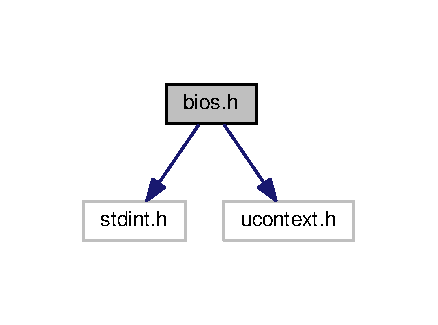
\includegraphics[width=210pt]{bios_8h__incl}
\end{center}
\end{figure}
This graph shows which files directly or indirectly include this file\+:\nopagebreak
\begin{figure}[H]
\begin{center}
\leavevmode
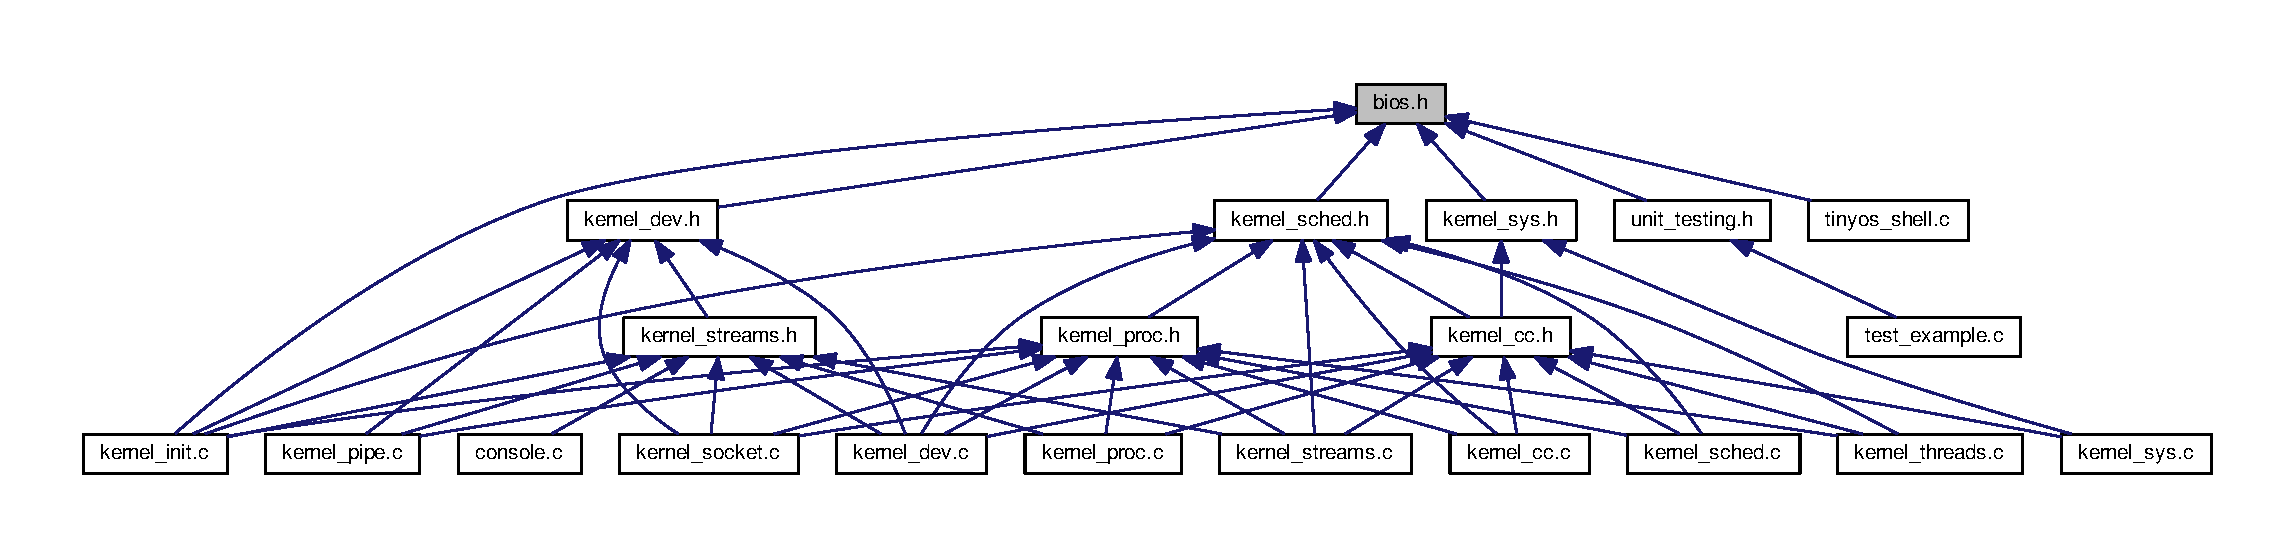
\includegraphics[width=350pt]{bios_8h__dep__incl}
\end{center}
\end{figure}
\subsection*{Macros}
\begin{DoxyCompactItemize}
\item 
\#define \hyperlink{bios_8h_a009855593b59738d24dbfc236edb3b14}{M\+A\+X\+\_\+\+C\+O\+R\+ES}~32\hypertarget{bios_8h_a009855593b59738d24dbfc236edb3b14}{}\label{bios_8h_a009855593b59738d24dbfc236edb3b14}

\begin{DoxyCompactList}\small\item\em Maximum number of cores for a virtual machine. \end{DoxyCompactList}\item 
\#define \hyperlink{bios_8h_a4e7d162c7c35103b42768ff4a5c73905}{M\+A\+X\+\_\+\+T\+E\+R\+M\+I\+N\+A\+LS}~4\hypertarget{bios_8h_a4e7d162c7c35103b42768ff4a5c73905}{}\label{bios_8h_a4e7d162c7c35103b42768ff4a5c73905}

\begin{DoxyCompactList}\small\item\em Maximum number of terminals for a virtual machine. \end{DoxyCompactList}\end{DoxyCompactItemize}
\subsection*{Typedefs}
\begin{DoxyCompactItemize}
\item 
typedef void \hyperlink{bios_8h_a11aeb47c6c66d331acd12556d0d4aedc}{interrupt\+\_\+handler}()\hypertarget{bios_8h_a11aeb47c6c66d331acd12556d0d4aedc}{}\label{bios_8h_a11aeb47c6c66d331acd12556d0d4aedc}

\begin{DoxyCompactList}\small\item\em The signature type of interrupt handlers. \end{DoxyCompactList}\item 
typedef unsigned int \hyperlink{bios_8h_a91ad9478d81a7aaf2593e8d9c3d06a14}{uint}\hypertarget{bios_8h_a91ad9478d81a7aaf2593e8d9c3d06a14}{}\label{bios_8h_a91ad9478d81a7aaf2593e8d9c3d06a14}

\begin{DoxyCompactList}\small\item\em Helper declaration. \end{DoxyCompactList}\item 
typedef uint64\+\_\+t \hyperlink{bios_8h_ae7291e5cd742fb9bc6d4aaa0d51bd0ee}{Timer\+Duration}\hypertarget{bios_8h_ae7291e5cd742fb9bc6d4aaa0d51bd0ee}{}\label{bios_8h_ae7291e5cd742fb9bc6d4aaa0d51bd0ee}

\begin{DoxyCompactList}\small\item\em A type for time intervals measured in microseconds. \end{DoxyCompactList}\item 
typedef enum \hyperlink{bios_8h_a137af7bce5ff764f5c0aa4550086deaa}{Interrupt} \hyperlink{bios_8h_a9d92c1d2b682bfedd88e238b6bf2fb22}{Interrupt}\hypertarget{bios_8h_a9d92c1d2b682bfedd88e238b6bf2fb22}{}\label{bios_8h_a9d92c1d2b682bfedd88e238b6bf2fb22}

\begin{DoxyCompactList}\small\item\em The interrupts supported by the C\+PU. \end{DoxyCompactList}\item 
typedef ucontext\+\_\+t \hyperlink{bios_8h_a6067c1395a75fc3e17f1ea6353065b54}{cpu\+\_\+context\+\_\+t}\hypertarget{bios_8h_a6067c1395a75fc3e17f1ea6353065b54}{}\label{bios_8h_a6067c1395a75fc3e17f1ea6353065b54}

\begin{DoxyCompactList}\small\item\em A type for saving C\+PU context into. \end{DoxyCompactList}\end{DoxyCompactItemize}
\subsection*{Enumerations}
\begin{DoxyCompactItemize}
\item 
enum \hyperlink{bios_8h_a137af7bce5ff764f5c0aa4550086deaa}{Interrupt} \{ \\*
\hyperlink{bios_8h_a137af7bce5ff764f5c0aa4550086deaaab4019255561cb4b48789d55c079e1709}{I\+CI}, 
\hyperlink{bios_8h_a137af7bce5ff764f5c0aa4550086deaaac4212312865bd8ac6810b9651d9e80df}{A\+L\+A\+RM}, 
\hyperlink{bios_8h_a137af7bce5ff764f5c0aa4550086deaaa2e06ea796d072595be1770c601e78206}{S\+E\+R\+I\+A\+L\+\_\+\+R\+X\+\_\+\+R\+E\+A\+DY}, 
\hyperlink{bios_8h_a137af7bce5ff764f5c0aa4550086deaaad168539d997c69c61da9c1f5f3187878}{S\+E\+R\+I\+A\+L\+\_\+\+T\+X\+\_\+\+R\+E\+A\+DY}, 
\\*
{\bfseries maximum\+\_\+interrupt\+\_\+no}
 \}\begin{DoxyCompactList}\small\item\em The interrupts supported by the C\+PU. \end{DoxyCompactList}
\end{DoxyCompactItemize}
\subsection*{Functions}
\begin{DoxyCompactItemize}
\item 
void \hyperlink{bios_8h_a3474751482bc2a9a40597f66fe35f630}{vm\+\_\+boot} (\hyperlink{bios_8h_a11aeb47c6c66d331acd12556d0d4aedc}{interrupt\+\_\+handler} bootfunc, \hyperlink{bios_8h_a91ad9478d81a7aaf2593e8d9c3d06a14}{uint} cores, \hyperlink{bios_8h_a91ad9478d81a7aaf2593e8d9c3d06a14}{uint} serialno)
\begin{DoxyCompactList}\small\item\em Boot a C\+PU with the given number of cores and boot function. \end{DoxyCompactList}\item 
\hyperlink{bios_8h_a91ad9478d81a7aaf2593e8d9c3d06a14}{uint} \hyperlink{bios_8h_aa02a29e5c8a1f4d68413eea0aaa09fba}{cpu\+\_\+cores} ()\hypertarget{bios_8h_aa02a29e5c8a1f4d68413eea0aaa09fba}{}\label{bios_8h_aa02a29e5c8a1f4d68413eea0aaa09fba}

\begin{DoxyCompactList}\small\item\em Returns the number of cores. \end{DoxyCompactList}\item 
void \hyperlink{bios_8h_ab8f96f6027a2276735b4a221a56ed786}{cpu\+\_\+core\+\_\+barrier\+\_\+sync} ()
\begin{DoxyCompactList}\small\item\em Barrier synchronization for all cores. \end{DoxyCompactList}\item 
void \hyperlink{bios_8h_a719b0f9f8854d21436c96931ba1caf59}{cpu\+\_\+ici} (\hyperlink{bios_8h_a91ad9478d81a7aaf2593e8d9c3d06a14}{uint} core)
\begin{DoxyCompactList}\small\item\em Raise an I\+CI interrupt to the given core. \end{DoxyCompactList}\item 
void \hyperlink{bios_8h_a0cf5c5e80f04d98362346e6ec770022d}{cpu\+\_\+interrupt\+\_\+handler} (\hyperlink{bios_8h_a137af7bce5ff764f5c0aa4550086deaa}{Interrupt} interrupt, \hyperlink{bios_8h_a11aeb47c6c66d331acd12556d0d4aedc}{interrupt\+\_\+handler} handler)
\begin{DoxyCompactList}\small\item\em Define an interrupt handler for this core. \end{DoxyCompactList}\item 
void \hyperlink{bios_8h_ab2be31ceb56ec6919d4d25fe4b2da0c8}{cpu\+\_\+disable\+\_\+interrupts} ()
\begin{DoxyCompactList}\small\item\em Disable interrupts for this core. \end{DoxyCompactList}\item 
void \hyperlink{bios_8h_a10055a90cf57a2a22fa9193922f9f2a8}{cpu\+\_\+enable\+\_\+interrupts} ()
\begin{DoxyCompactList}\small\item\em Enable interrupts for this core. \end{DoxyCompactList}\item 
void \hyperlink{bios_8h_a3e2c9a3aea40c8eeaa723ee35caace06}{cpu\+\_\+core\+\_\+halt} ()
\begin{DoxyCompactList}\small\item\em Halt the core until an interrupt arrives. \end{DoxyCompactList}\item 
void \hyperlink{bios_8h_a9191a31f24c07b8282a3c8edbba24ee0}{cpu\+\_\+core\+\_\+restart} (\hyperlink{bios_8h_a91ad9478d81a7aaf2593e8d9c3d06a14}{uint} c)
\begin{DoxyCompactList}\small\item\em Restart the given core. \end{DoxyCompactList}\item 
void \hyperlink{bios_8h_a7eeccd43040cc43ac977f649d639a3e9}{cpu\+\_\+core\+\_\+restart\+\_\+one} ()
\begin{DoxyCompactList}\small\item\em Restart some halted core. \end{DoxyCompactList}\item 
void \hyperlink{bios_8h_aa82b1a876663da26cbf511bcfb06404d}{cpu\+\_\+core\+\_\+restart\+\_\+all} ()
\begin{DoxyCompactList}\small\item\em Signal all halted cores to restart. \end{DoxyCompactList}\item 
void \hyperlink{bios_8h_a825ac4a4bcf2ef8d3c9bb48d5434c161}{cpu\+\_\+initialize\+\_\+context} (\hyperlink{bios_8h_a6067c1395a75fc3e17f1ea6353065b54}{cpu\+\_\+context\+\_\+t} $\ast$ctx, void $\ast$ss\+\_\+sp, size\+\_\+t ss\+\_\+size, void($\ast$func)())
\begin{DoxyCompactList}\small\item\em Initialize a C\+PU context for a new thread. \end{DoxyCompactList}\item 
void \hyperlink{bios_8h_a78a3870d56e6867224909cf226c2e90a}{cpu\+\_\+swap\+\_\+context} (\hyperlink{bios_8h_a6067c1395a75fc3e17f1ea6353065b54}{cpu\+\_\+context\+\_\+t} $\ast$oldctx, \hyperlink{bios_8h_a6067c1395a75fc3e17f1ea6353065b54}{cpu\+\_\+context\+\_\+t} $\ast$newctx)
\begin{DoxyCompactList}\small\item\em Switch the C\+PU context. \end{DoxyCompactList}\item 
\hyperlink{bios_8h_ae7291e5cd742fb9bc6d4aaa0d51bd0ee}{Timer\+Duration} \hyperlink{bios_8h_a01f7a35679bdda42fff3da6ae6e5664b}{bios\+\_\+set\+\_\+timer} (\hyperlink{bios_8h_ae7291e5cd742fb9bc6d4aaa0d51bd0ee}{Timer\+Duration} usec)
\begin{DoxyCompactList}\small\item\em Reset the core timer to the specified interval. \end{DoxyCompactList}\item 
\hyperlink{bios_8h_ae7291e5cd742fb9bc6d4aaa0d51bd0ee}{Timer\+Duration} \hyperlink{bios_8h_a27768c037d72b51415b836bd93196df2}{bios\+\_\+cancel\+\_\+timer} ()
\begin{DoxyCompactList}\small\item\em Cancel the current activated timer, if any. \end{DoxyCompactList}\item 
\hyperlink{bios_8h_ae7291e5cd742fb9bc6d4aaa0d51bd0ee}{Timer\+Duration} \hyperlink{bios_8h_a78addcd72c31fb32d46cc51fe01a86b4}{bios\+\_\+clock} ()
\begin{DoxyCompactList}\small\item\em Get the current time from the hardware clock. \end{DoxyCompactList}\item 
\hyperlink{bios_8h_a91ad9478d81a7aaf2593e8d9c3d06a14}{uint} \hyperlink{bios_8h_af69405820033d3f2e8033af258f47ea2}{bios\+\_\+serial\+\_\+ports} ()
\begin{DoxyCompactList}\small\item\em Return the number of serial ports/terminals. \end{DoxyCompactList}\item 
void \hyperlink{bios_8h_a3d9df4f1db5a1d99720f327668726e2b}{bios\+\_\+serial\+\_\+interrupt\+\_\+core} (\hyperlink{bios_8h_a91ad9478d81a7aaf2593e8d9c3d06a14}{uint} serial, \hyperlink{bios_8h_a137af7bce5ff764f5c0aa4550086deaa}{Interrupt} intno, \hyperlink{bios_8h_a91ad9478d81a7aaf2593e8d9c3d06a14}{uint} core)
\begin{DoxyCompactList}\small\item\em Assign a core to interrupts from a specific serial device. \end{DoxyCompactList}\item 
int \hyperlink{bios_8h_a04ebe8b1d424c0ef473db751f7b79fbb}{bios\+\_\+read\+\_\+serial} (\hyperlink{bios_8h_a91ad9478d81a7aaf2593e8d9c3d06a14}{uint} serial, char $\ast$ptr)
\begin{DoxyCompactList}\small\item\em Read a byte from a serial port. \end{DoxyCompactList}\item 
int \hyperlink{bios_8h_a97bde2ebd5f9d86c0085aacaa5e5d287}{bios\+\_\+write\+\_\+serial} (\hyperlink{bios_8h_a91ad9478d81a7aaf2593e8d9c3d06a14}{uint} serial, char value)
\begin{DoxyCompactList}\small\item\em Write a byte to a serial port. \end{DoxyCompactList}\end{DoxyCompactItemize}
\subsection*{Variables}
\begin{DoxyCompactItemize}
\item 
\+\_\+\+Thread\+\_\+local \hyperlink{bios_8h_a91ad9478d81a7aaf2593e8d9c3d06a14}{uint} \hyperlink{bios_8h_abac58ced7d51f54f2318b326bc991933}{cpu\+\_\+core\+\_\+id}\hypertarget{bios_8h_abac58ced7d51f54f2318b326bc991933}{}\label{bios_8h_abac58ced7d51f54f2318b326bc991933}

\begin{DoxyCompactList}\small\item\em Contains the id of the current core. \end{DoxyCompactList}\end{DoxyCompactItemize}


\subsection{Detailed Description}
The Virtual Machine A\+PI. 

This file contains the A\+PI for a virtual machine (simulated computer) which we will refer to as VM. This VM is used to implement tinyos3 on.

The VM has a multicore C\+PU and peripherals.

A simulation starts by calling function {\ttfamily vm\+\_\+boot}. The description of the VM (currently, the number of simulated cores and the number of terminal devices), and also the initial function executed by each core at boot time, are given as arguments.

The VM (virtual) hardware is controlled by a B\+I\+OS (Basic I/O System) through the B\+I\+OS A\+PI. We now describe the concepts of the B\+I\+OS in detail.

\subsubsection*{C\+PU }

A C\+PU has 1 or more cores. Each core executes independently of each other. Variable cpu\+\_\+core\+\_\+id contains the id number of the current core.

\subsubsection*{Interrupts }

Each C\+PU core has its own interrupt vector---it can set its own interrupt handlers, independently of other cores. Setting an interrupt handler to {\ttfamily N\+U\+LL} (the default), ignores the interrupt for this core.


\begin{DoxyItemize}
\item When an interrupt handler executes, interrupts are initially disabled.
\item Interrupts can also be enabled and disabled programmatically.
\item If an interrupt is raised while interrupts are disabled, it will be marked as raised and the interrupt handler (if non-\/\+N\+U\+LL) will be called as soon as interrupts are re-\/enabled.
\item The {\bfseries I\+CI} (Inter-\/\+Core Interrupt) interrupt can be sent from one core to another (or to itself!).
\end{DoxyItemize}

\subsubsection*{Peripherals }

The peripherals are managed via the \textquotesingle{}bios\+\_\+...\textquotesingle{} functions.

There are two types of simulated peripherals\+: {\itshape timers} and {\itshape serial ports} (connected to terminals). Each type of peripheral is documented below.

\subsubsection*{Timers }

Each simulated core has its own timer. A timer can be activated by initializing it with some time interval. When the timer expires, the A\+L\+A\+RM interrupt is raised for the core.

\subsubsection*{Serial ports }

The virtual machine has a number of serial ports connected to terminals.

Each serial port/terminal can support reading and writing of single bytes. The reads return keyboard input, whereas the writes send characters to display on the screen.

Terminals are numbered from 0, up to {\ttfamily M\+A\+X\+\_\+\+T\+E\+R\+M\+I\+N\+A\+L\+S-\/1}.

Implementation-\/wise, for each terminal/serial port, two Unix named pipes must exist in the current directory\+: one named con $ N $ and one named kbd $ N $, where $ N $ is the number of the serial port. For example, if the computer has 2 serial ports, the following named pipes must be defined in the current directory at runtime\+: con0 kbd0 con1 kbd1

Also, program \textquotesingle{}terminal\textquotesingle{} must be executed twice (in two different windows)\+:

./terminal 0

./terminal 1

Data can be read from a serial port, one byte at a time. A read may fail if the device is not-\/ready to perform the operation. On a device which is ready, the read will succeed. When a non-\/ready device becomes ready, a {\ttfamily S\+E\+R\+I\+A\+L\+\_\+\+R\+X\+\_\+\+R\+E\+A\+DY} interrupt is raised.

Data can be written to a serial port, one byte at a time. A write may fail if the device is not-\/ready to perform the operation. On a device which is ready, the write will succeed. When a non-\/ready device becomes ready, a {\ttfamily S\+E\+R\+I\+A\+L\+\_\+\+T\+X\+\_\+\+R\+E\+A\+DY} interrupt is raised.

Also, each interrupt is sent if the serial device timeouts (is inactive for about 300 msec). 

\subsection{Enumeration Type Documentation}
\index{bios.\+h@{bios.\+h}!Interrupt@{Interrupt}}
\index{Interrupt@{Interrupt}!bios.\+h@{bios.\+h}}
\subsubsection[{\texorpdfstring{Interrupt}{Interrupt}}]{\setlength{\rightskip}{0pt plus 5cm}enum {\bf Interrupt}}\hypertarget{bios_8h_a137af7bce5ff764f5c0aa4550086deaa}{}\label{bios_8h_a137af7bce5ff764f5c0aa4550086deaa}


The interrupts supported by the C\+PU. 

\begin{Desc}
\item[Enumerator]\par
\begin{description}
\index{I\+CI@{I\+CI}!bios.\+h@{bios.\+h}}\index{bios.\+h@{bios.\+h}!I\+CI@{I\+CI}}\item[{\em 
I\+CI\hypertarget{bios_8h_a137af7bce5ff764f5c0aa4550086deaaab4019255561cb4b48789d55c079e1709}{}\label{bios_8h_a137af7bce5ff764f5c0aa4550086deaaab4019255561cb4b48789d55c079e1709}
}]Raised by some core, via \hyperlink{bios_8h_a719b0f9f8854d21436c96931ba1caf59}{cpu\+\_\+ici()} \index{A\+L\+A\+RM@{A\+L\+A\+RM}!bios.\+h@{bios.\+h}}\index{bios.\+h@{bios.\+h}!A\+L\+A\+RM@{A\+L\+A\+RM}}\item[{\em 
A\+L\+A\+RM\hypertarget{bios_8h_a137af7bce5ff764f5c0aa4550086deaaac4212312865bd8ac6810b9651d9e80df}{}\label{bios_8h_a137af7bce5ff764f5c0aa4550086deaaac4212312865bd8ac6810b9651d9e80df}
}]Raised when the core\textquotesingle{}s timer expires. \index{S\+E\+R\+I\+A\+L\+\_\+\+R\+X\+\_\+\+R\+E\+A\+DY@{S\+E\+R\+I\+A\+L\+\_\+\+R\+X\+\_\+\+R\+E\+A\+DY}!bios.\+h@{bios.\+h}}\index{bios.\+h@{bios.\+h}!S\+E\+R\+I\+A\+L\+\_\+\+R\+X\+\_\+\+R\+E\+A\+DY@{S\+E\+R\+I\+A\+L\+\_\+\+R\+X\+\_\+\+R\+E\+A\+DY}}\item[{\em 
S\+E\+R\+I\+A\+L\+\_\+\+R\+X\+\_\+\+R\+E\+A\+DY\hypertarget{bios_8h_a137af7bce5ff764f5c0aa4550086deaaa2e06ea796d072595be1770c601e78206}{}\label{bios_8h_a137af7bce5ff764f5c0aa4550086deaaa2e06ea796d072595be1770c601e78206}
}]Raised when data is available for reading from a serial port \index{S\+E\+R\+I\+A\+L\+\_\+\+T\+X\+\_\+\+R\+E\+A\+DY@{S\+E\+R\+I\+A\+L\+\_\+\+T\+X\+\_\+\+R\+E\+A\+DY}!bios.\+h@{bios.\+h}}\index{bios.\+h@{bios.\+h}!S\+E\+R\+I\+A\+L\+\_\+\+T\+X\+\_\+\+R\+E\+A\+DY@{S\+E\+R\+I\+A\+L\+\_\+\+T\+X\+\_\+\+R\+E\+A\+DY}}\item[{\em 
S\+E\+R\+I\+A\+L\+\_\+\+T\+X\+\_\+\+R\+E\+A\+DY\hypertarget{bios_8h_a137af7bce5ff764f5c0aa4550086deaaad168539d997c69c61da9c1f5f3187878}{}\label{bios_8h_a137af7bce5ff764f5c0aa4550086deaaad168539d997c69c61da9c1f5f3187878}
}]Raised when a serial port is ready to accept data \end{description}
\end{Desc}


Definition at line 117 of file bios.\+h.



\subsection{Function Documentation}
\index{bios.\+h@{bios.\+h}!bios\+\_\+cancel\+\_\+timer@{bios\+\_\+cancel\+\_\+timer}}
\index{bios\+\_\+cancel\+\_\+timer@{bios\+\_\+cancel\+\_\+timer}!bios.\+h@{bios.\+h}}
\subsubsection[{\texorpdfstring{bios\+\_\+cancel\+\_\+timer()}{bios_cancel_timer()}}]{\setlength{\rightskip}{0pt plus 5cm}{\bf Timer\+Duration} bios\+\_\+cancel\+\_\+timer (
\begin{DoxyParamCaption}
{}
\end{DoxyParamCaption}
)}\hypertarget{bios_8h_a27768c037d72b51415b836bd93196df2}{}\label{bios_8h_a27768c037d72b51415b836bd93196df2}


Cancel the current activated timer, if any. 

This can be called even if the timer is not already activated. This call is equivalent to bios\+\_\+set\+\_\+timer(0).

\begin{DoxySeeAlso}{See also}
\hyperlink{bios_8h_a01f7a35679bdda42fff3da6ae6e5664b}{bios\+\_\+set\+\_\+timer} 
\end{DoxySeeAlso}
\index{bios.\+h@{bios.\+h}!bios\+\_\+clock@{bios\+\_\+clock}}
\index{bios\+\_\+clock@{bios\+\_\+clock}!bios.\+h@{bios.\+h}}
\subsubsection[{\texorpdfstring{bios\+\_\+clock()}{bios_clock()}}]{\setlength{\rightskip}{0pt plus 5cm}{\bf Timer\+Duration} bios\+\_\+clock (
\begin{DoxyParamCaption}
{}
\end{DoxyParamCaption}
)}\hypertarget{bios_8h_a78addcd72c31fb32d46cc51fe01a86b4}{}\label{bios_8h_a78addcd72c31fb32d46cc51fe01a86b4}


Get the current time from the hardware clock. 

This function returns a real-\/time clock value, in usec. The value of the clock is 10 times the number of seconds since the epoch.

The resolution of the clock is very low, currently around 100 msec. Therefore, it is inappropriate for any type of precise timing. \index{bios.\+h@{bios.\+h}!bios\+\_\+read\+\_\+serial@{bios\+\_\+read\+\_\+serial}}
\index{bios\+\_\+read\+\_\+serial@{bios\+\_\+read\+\_\+serial}!bios.\+h@{bios.\+h}}
\subsubsection[{\texorpdfstring{bios\+\_\+read\+\_\+serial(uint serial, char $\ast$ptr)}{bios_read_serial(uint serial, char *ptr)}}]{\setlength{\rightskip}{0pt plus 5cm}int bios\+\_\+read\+\_\+serial (
\begin{DoxyParamCaption}
\item[{{\bf uint}}]{serial, }
\item[{char $\ast$}]{ptr}
\end{DoxyParamCaption}
)}\hypertarget{bios_8h_a04ebe8b1d424c0ef473db751f7b79fbb}{}\label{bios_8h_a04ebe8b1d424c0ef473db751f7b79fbb}


Read a byte from a serial port. 

Try to read a byte from serial port {\ttfamily serial} and store it into the location pointed by {\ttfamily ptr}. If the operation succeds, 1 is returned. If not, 0 is returned. The operation may not succeed, if the terminal connected to the serial port has not sent any data.

If this operation returns 0, a {\ttfamily S\+E\+R\+I\+A\+L\+\_\+\+R\+X\+\_\+\+R\+E\+A\+DY} interrupt will be raised when data is ready to be received, but the contents of {\ttfamily $\ast$ptr} will not be touched.


\begin{DoxyParams}{Parameters}
{\em serial} & the serial device to read from \\
\hline
{\em ptr} & the location in which to store the read byte \\
\hline
\end{DoxyParams}
\begin{DoxyReturn}{Returns}
a integer designating success (non-\/zero) or failure (zero) 
\end{DoxyReturn}
\index{bios.\+h@{bios.\+h}!bios\+\_\+serial\+\_\+interrupt\+\_\+core@{bios\+\_\+serial\+\_\+interrupt\+\_\+core}}
\index{bios\+\_\+serial\+\_\+interrupt\+\_\+core@{bios\+\_\+serial\+\_\+interrupt\+\_\+core}!bios.\+h@{bios.\+h}}
\subsubsection[{\texorpdfstring{bios\+\_\+serial\+\_\+interrupt\+\_\+core(uint serial, Interrupt intno, uint core)}{bios_serial_interrupt_core(uint serial, Interrupt intno, uint core)}}]{\setlength{\rightskip}{0pt plus 5cm}void bios\+\_\+serial\+\_\+interrupt\+\_\+core (
\begin{DoxyParamCaption}
\item[{{\bf uint}}]{serial, }
\item[{{\bf Interrupt}}]{intno, }
\item[{{\bf uint}}]{core}
\end{DoxyParamCaption}
)}\hypertarget{bios_8h_a3d9df4f1db5a1d99720f327668726e2b}{}\label{bios_8h_a3d9df4f1db5a1d99720f327668726e2b}


Assign a core to interrupts from a specific serial device. 

Make interrupts of type {\ttfamily intno} for serial port port {\ttfamily serial} be sent to {\ttfamily core}. By default, initially all interrupts are sent to core 0.


\begin{DoxyParams}{Parameters}
{\em serial} & the serial device whose interrupt is assigned, it must be greater of equal to {\ttfamily 0} and less than {\ttfamily \hyperlink{bios_8h_af69405820033d3f2e8033af258f47ea2}{bios\+\_\+serial\+\_\+ports()}}. \\
\hline
{\em intno} & the interrupt to assign (one of {\ttfamily S\+E\+R\+I\+A\+L\+\_\+\+R\+X\+\_\+\+R\+E\+A\+DY} and {\ttfamily S\+E\+R\+I\+A\+L\+\_\+\+T\+X\+\_\+\+R\+E\+A\+DY}) \\
\hline
{\em core} & th \\
\hline
\end{DoxyParams}
\index{bios.\+h@{bios.\+h}!bios\+\_\+serial\+\_\+ports@{bios\+\_\+serial\+\_\+ports}}
\index{bios\+\_\+serial\+\_\+ports@{bios\+\_\+serial\+\_\+ports}!bios.\+h@{bios.\+h}}
\subsubsection[{\texorpdfstring{bios\+\_\+serial\+\_\+ports()}{bios_serial_ports()}}]{\setlength{\rightskip}{0pt plus 5cm}{\bf uint} bios\+\_\+serial\+\_\+ports (
\begin{DoxyParamCaption}
{}
\end{DoxyParamCaption}
)}\hypertarget{bios_8h_af69405820033d3f2e8033af258f47ea2}{}\label{bios_8h_af69405820033d3f2e8033af258f47ea2}


Return the number of serial ports/terminals. 

This is the number specified at the initialization of the VM. \index{bios.\+h@{bios.\+h}!bios\+\_\+set\+\_\+timer@{bios\+\_\+set\+\_\+timer}}
\index{bios\+\_\+set\+\_\+timer@{bios\+\_\+set\+\_\+timer}!bios.\+h@{bios.\+h}}
\subsubsection[{\texorpdfstring{bios\+\_\+set\+\_\+timer(\+Timer\+Duration usec)}{bios_set_timer(TimerDuration usec)}}]{\setlength{\rightskip}{0pt plus 5cm}{\bf Timer\+Duration} bios\+\_\+set\+\_\+timer (
\begin{DoxyParamCaption}
\item[{{\bf Timer\+Duration}}]{usec}
\end{DoxyParamCaption}
)}\hypertarget{bios_8h_a01f7a35679bdda42fff3da6ae6e5664b}{}\label{bios_8h_a01f7a35679bdda42fff3da6ae6e5664b}


Reset the core timer to the specified interval. 

The interval for the timer is given in microseconds, but the accuracy of the alarm is much coarser, to the order of 10 msec (that is, 10,000 microseconds). After the interval expires, the core receives an A\+L\+A\+RM interrupt.

This function can be called even if the timer is already activated; in this case, the previous timer countdown is canceled and the timer resets to the new value.

If {\ttfamily usec} is specified as 0, any existing timer count is canceled.


\begin{DoxyParams}{Parameters}
{\em usec} & the timer countdown interval in microseconds \\
\hline
\end{DoxyParams}
\begin{DoxyReturn}{Returns}
the time remaining interval since the last call 
\end{DoxyReturn}
\begin{DoxySeeAlso}{See also}
\hyperlink{bios_8h_a27768c037d72b51415b836bd93196df2}{bios\+\_\+cancel\+\_\+timer} 
\end{DoxySeeAlso}
\index{bios.\+h@{bios.\+h}!bios\+\_\+write\+\_\+serial@{bios\+\_\+write\+\_\+serial}}
\index{bios\+\_\+write\+\_\+serial@{bios\+\_\+write\+\_\+serial}!bios.\+h@{bios.\+h}}
\subsubsection[{\texorpdfstring{bios\+\_\+write\+\_\+serial(uint serial, char value)}{bios_write_serial(uint serial, char value)}}]{\setlength{\rightskip}{0pt plus 5cm}int bios\+\_\+write\+\_\+serial (
\begin{DoxyParamCaption}
\item[{{\bf uint}}]{serial, }
\item[{char}]{value}
\end{DoxyParamCaption}
)}\hypertarget{bios_8h_a97bde2ebd5f9d86c0085aacaa5e5d287}{}\label{bios_8h_a97bde2ebd5f9d86c0085aacaa5e5d287}


Write a byte to a serial port. 

Try to write byte {\ttfamily value} to serial port {\ttfamily serial}. If the operation succeds, 1 is returned. If not, 0 is returned.

If this operation returns 0, a {\ttfamily S\+E\+R\+I\+A\+L\+\_\+\+T\+X\+\_\+\+R\+E\+A\+DY} interrupt will be raised when the device is ready to accept data.


\begin{DoxyParams}{Parameters}
{\em serial} & the serial device to write to \\
\hline
{\em value} & the value to send to the serial device \\
\hline
\end{DoxyParams}
\begin{DoxyReturn}{Returns}
a integer designating success (non-\/zero) or failure (zero) 
\end{DoxyReturn}
\index{bios.\+h@{bios.\+h}!cpu\+\_\+core\+\_\+barrier\+\_\+sync@{cpu\+\_\+core\+\_\+barrier\+\_\+sync}}
\index{cpu\+\_\+core\+\_\+barrier\+\_\+sync@{cpu\+\_\+core\+\_\+barrier\+\_\+sync}!bios.\+h@{bios.\+h}}
\subsubsection[{\texorpdfstring{cpu\+\_\+core\+\_\+barrier\+\_\+sync()}{cpu_core_barrier_sync()}}]{\setlength{\rightskip}{0pt plus 5cm}void cpu\+\_\+core\+\_\+barrier\+\_\+sync (
\begin{DoxyParamCaption}
{}
\end{DoxyParamCaption}
)}\hypertarget{bios_8h_ab8f96f6027a2276735b4a221a56ed786}{}\label{bios_8h_ab8f96f6027a2276735b4a221a56ed786}


Barrier synchronization for all cores. 

Each core calling this function stops, until all cores have called it. Then, all cores proceed.

This is mostly useful when the machine boots the operating system, or at shutdown. \index{bios.\+h@{bios.\+h}!cpu\+\_\+core\+\_\+halt@{cpu\+\_\+core\+\_\+halt}}
\index{cpu\+\_\+core\+\_\+halt@{cpu\+\_\+core\+\_\+halt}!bios.\+h@{bios.\+h}}
\subsubsection[{\texorpdfstring{cpu\+\_\+core\+\_\+halt()}{cpu_core_halt()}}]{\setlength{\rightskip}{0pt plus 5cm}void cpu\+\_\+core\+\_\+halt (
\begin{DoxyParamCaption}
{}
\end{DoxyParamCaption}
)}\hypertarget{bios_8h_a3e2c9a3aea40c8eeaa723ee35caace06}{}\label{bios_8h_a3e2c9a3aea40c8eeaa723ee35caace06}


Halt the core until an interrupt arrives. 

This function will block the core on which it is called, until an interrupt arrives for the core.

This function is useful when a core becomes idle. An idle core does not consume simulation resources (in particular C\+PU time). \index{bios.\+h@{bios.\+h}!cpu\+\_\+core\+\_\+restart@{cpu\+\_\+core\+\_\+restart}}
\index{cpu\+\_\+core\+\_\+restart@{cpu\+\_\+core\+\_\+restart}!bios.\+h@{bios.\+h}}
\subsubsection[{\texorpdfstring{cpu\+\_\+core\+\_\+restart(uint c)}{cpu_core_restart(uint c)}}]{\setlength{\rightskip}{0pt plus 5cm}void cpu\+\_\+core\+\_\+restart (
\begin{DoxyParamCaption}
\item[{{\bf uint}}]{c}
\end{DoxyParamCaption}
)}\hypertarget{bios_8h_a9191a31f24c07b8282a3c8edbba24ee0}{}\label{bios_8h_a9191a31f24c07b8282a3c8edbba24ee0}


Restart the given core. 

This call will restart the given core, if it was halted. 
\begin{DoxyParams}{Parameters}
{\em c} & the core to restart \\
\hline
\end{DoxyParams}
\index{bios.\+h@{bios.\+h}!cpu\+\_\+core\+\_\+restart\+\_\+all@{cpu\+\_\+core\+\_\+restart\+\_\+all}}
\index{cpu\+\_\+core\+\_\+restart\+\_\+all@{cpu\+\_\+core\+\_\+restart\+\_\+all}!bios.\+h@{bios.\+h}}
\subsubsection[{\texorpdfstring{cpu\+\_\+core\+\_\+restart\+\_\+all()}{cpu_core_restart_all()}}]{\setlength{\rightskip}{0pt plus 5cm}void cpu\+\_\+core\+\_\+restart\+\_\+all (
\begin{DoxyParamCaption}
{}
\end{DoxyParamCaption}
)}\hypertarget{bios_8h_aa82b1a876663da26cbf511bcfb06404d}{}\label{bios_8h_aa82b1a876663da26cbf511bcfb06404d}


Signal all halted cores to restart. 

When this function is called, all halted cores will be restarted. \index{bios.\+h@{bios.\+h}!cpu\+\_\+core\+\_\+restart\+\_\+one@{cpu\+\_\+core\+\_\+restart\+\_\+one}}
\index{cpu\+\_\+core\+\_\+restart\+\_\+one@{cpu\+\_\+core\+\_\+restart\+\_\+one}!bios.\+h@{bios.\+h}}
\subsubsection[{\texorpdfstring{cpu\+\_\+core\+\_\+restart\+\_\+one()}{cpu_core_restart_one()}}]{\setlength{\rightskip}{0pt plus 5cm}void cpu\+\_\+core\+\_\+restart\+\_\+one (
\begin{DoxyParamCaption}
{}
\end{DoxyParamCaption}
)}\hypertarget{bios_8h_a7eeccd43040cc43ac977f649d639a3e9}{}\label{bios_8h_a7eeccd43040cc43ac977f649d639a3e9}


Restart some halted core. 

This call will restart some halted core, if at least one exists. \index{bios.\+h@{bios.\+h}!cpu\+\_\+disable\+\_\+interrupts@{cpu\+\_\+disable\+\_\+interrupts}}
\index{cpu\+\_\+disable\+\_\+interrupts@{cpu\+\_\+disable\+\_\+interrupts}!bios.\+h@{bios.\+h}}
\subsubsection[{\texorpdfstring{cpu\+\_\+disable\+\_\+interrupts()}{cpu_disable_interrupts()}}]{\setlength{\rightskip}{0pt plus 5cm}void cpu\+\_\+disable\+\_\+interrupts (
\begin{DoxyParamCaption}
{}
\end{DoxyParamCaption}
)}\hypertarget{bios_8h_ab2be31ceb56ec6919d4d25fe4b2da0c8}{}\label{bios_8h_ab2be31ceb56ec6919d4d25fe4b2da0c8}


Disable interrupts for this core. 

If an interrupt arrives while interrupts are disabled, it will be marked as {\itshape pending} and will be raised when interrupts are re-\/enabled.

\begin{DoxySeeAlso}{See also}
\hyperlink{bios_8h_a10055a90cf57a2a22fa9193922f9f2a8}{cpu\+\_\+enable\+\_\+interrupts} 
\end{DoxySeeAlso}
\index{bios.\+h@{bios.\+h}!cpu\+\_\+enable\+\_\+interrupts@{cpu\+\_\+enable\+\_\+interrupts}}
\index{cpu\+\_\+enable\+\_\+interrupts@{cpu\+\_\+enable\+\_\+interrupts}!bios.\+h@{bios.\+h}}
\subsubsection[{\texorpdfstring{cpu\+\_\+enable\+\_\+interrupts()}{cpu_enable_interrupts()}}]{\setlength{\rightskip}{0pt plus 5cm}void cpu\+\_\+enable\+\_\+interrupts (
\begin{DoxyParamCaption}
{}
\end{DoxyParamCaption}
)}\hypertarget{bios_8h_a10055a90cf57a2a22fa9193922f9f2a8}{}\label{bios_8h_a10055a90cf57a2a22fa9193922f9f2a8}


Enable interrupts for this core. 

If an interrupt is pending, i.\+e., it arrived while interrupts were disabled, it will be raised as soon as this call is made.

\begin{DoxySeeAlso}{See also}
\hyperlink{bios_8h_ab2be31ceb56ec6919d4d25fe4b2da0c8}{cpu\+\_\+disable\+\_\+interrupts} 
\end{DoxySeeAlso}
\index{bios.\+h@{bios.\+h}!cpu\+\_\+ici@{cpu\+\_\+ici}}
\index{cpu\+\_\+ici@{cpu\+\_\+ici}!bios.\+h@{bios.\+h}}
\subsubsection[{\texorpdfstring{cpu\+\_\+ici(uint core)}{cpu_ici(uint core)}}]{\setlength{\rightskip}{0pt plus 5cm}void cpu\+\_\+ici (
\begin{DoxyParamCaption}
\item[{{\bf uint}}]{core}
\end{DoxyParamCaption}
)}\hypertarget{bios_8h_a719b0f9f8854d21436c96931ba1caf59}{}\label{bios_8h_a719b0f9f8854d21436c96931ba1caf59}


Raise an I\+CI interrupt to the given core. 

This is a simple way that one core may interrupt another. \index{bios.\+h@{bios.\+h}!cpu\+\_\+initialize\+\_\+context@{cpu\+\_\+initialize\+\_\+context}}
\index{cpu\+\_\+initialize\+\_\+context@{cpu\+\_\+initialize\+\_\+context}!bios.\+h@{bios.\+h}}
\subsubsection[{\texorpdfstring{cpu\+\_\+initialize\+\_\+context(cpu\+\_\+context\+\_\+t $\ast$ctx, void $\ast$ss\+\_\+sp, size\+\_\+t ss\+\_\+size, void($\ast$func)())}{cpu_initialize_context(cpu_context_t *ctx, void *ss_sp, size_t ss_size, void(*func)())}}]{\setlength{\rightskip}{0pt plus 5cm}void cpu\+\_\+initialize\+\_\+context (
\begin{DoxyParamCaption}
\item[{{\bf cpu\+\_\+context\+\_\+t} $\ast$}]{ctx, }
\item[{void $\ast$}]{ss\+\_\+sp, }
\item[{size\+\_\+t}]{ss\+\_\+size, }
\item[{void($\ast$)()}]{func}
\end{DoxyParamCaption}
)}\hypertarget{bios_8h_a825ac4a4bcf2ef8d3c9bb48d5434c161}{}\label{bios_8h_a825ac4a4bcf2ef8d3c9bb48d5434c161}


Initialize a C\+PU context for a new thread. 

To initialize the context, a stack segment of adequate size must be provided.


\begin{DoxyParams}{Parameters}
{\em ctx} & the context object to initialize \\
\hline
{\em ss\+\_\+sp} & the pointer to the beginning of the stack segment \\
\hline
{\em ss\+\_\+size} & the size of the stack segment \\
\hline
{\em func} & the function to execute in the new context \\
\hline
\end{DoxyParams}
\index{bios.\+h@{bios.\+h}!cpu\+\_\+interrupt\+\_\+handler@{cpu\+\_\+interrupt\+\_\+handler}}
\index{cpu\+\_\+interrupt\+\_\+handler@{cpu\+\_\+interrupt\+\_\+handler}!bios.\+h@{bios.\+h}}
\subsubsection[{\texorpdfstring{cpu\+\_\+interrupt\+\_\+handler(\+Interrupt interrupt, interrupt\+\_\+handler handler)}{cpu_interrupt_handler(Interrupt interrupt, interrupt_handler handler)}}]{\setlength{\rightskip}{0pt plus 5cm}void cpu\+\_\+interrupt\+\_\+handler (
\begin{DoxyParamCaption}
\item[{{\bf Interrupt}}]{interrupt, }
\item[{{\bf interrupt\+\_\+handler}}]{handler}
\end{DoxyParamCaption}
)}\hypertarget{bios_8h_a0cf5c5e80f04d98362346e6ec770022d}{}\label{bios_8h_a0cf5c5e80f04d98362346e6ec770022d}


Define an interrupt handler for this core. 

This function set the interrupt handler of the calling core, for the given interrupt. If {\ttfamily handler} is N\+U\+LL, then the interrupt will be ignored by this core.


\begin{DoxyParams}{Parameters}
{\em interrupt} & the interrupt to set the handler for \\
\hline
{\em handler} & the handler function to call\\
\hline
\end{DoxyParams}
\begin{DoxySeeAlso}{See also}
\hyperlink{bios_8h_a11aeb47c6c66d331acd12556d0d4aedc}{interrupt\+\_\+handler} 

\hyperlink{bios_8h_a137af7bce5ff764f5c0aa4550086deaa}{Interrupt} 
\end{DoxySeeAlso}
\index{bios.\+h@{bios.\+h}!cpu\+\_\+swap\+\_\+context@{cpu\+\_\+swap\+\_\+context}}
\index{cpu\+\_\+swap\+\_\+context@{cpu\+\_\+swap\+\_\+context}!bios.\+h@{bios.\+h}}
\subsubsection[{\texorpdfstring{cpu\+\_\+swap\+\_\+context(cpu\+\_\+context\+\_\+t $\ast$oldctx, cpu\+\_\+context\+\_\+t $\ast$newctx)}{cpu_swap_context(cpu_context_t *oldctx, cpu_context_t *newctx)}}]{\setlength{\rightskip}{0pt plus 5cm}void cpu\+\_\+swap\+\_\+context (
\begin{DoxyParamCaption}
\item[{{\bf cpu\+\_\+context\+\_\+t} $\ast$}]{oldctx, }
\item[{{\bf cpu\+\_\+context\+\_\+t} $\ast$}]{newctx}
\end{DoxyParamCaption}
)}\hypertarget{bios_8h_a78a3870d56e6867224909cf226c2e90a}{}\label{bios_8h_a78a3870d56e6867224909cf226c2e90a}


Switch the C\+PU context. 

Save the current context into {\ttfamily oldctx} and load the contents of {\ttfamily newctx} into the C\+PU.


\begin{DoxyParams}{Parameters}
{\em oldctx} & pointer to the storage for the old context \\
\hline
{\em newctx} & pointer to the new context to be loaded \\
\hline
\end{DoxyParams}
\index{bios.\+h@{bios.\+h}!vm\+\_\+boot@{vm\+\_\+boot}}
\index{vm\+\_\+boot@{vm\+\_\+boot}!bios.\+h@{bios.\+h}}
\subsubsection[{\texorpdfstring{vm\+\_\+boot(interrupt\+\_\+handler bootfunc, uint cores, uint serialno)}{vm_boot(interrupt_handler bootfunc, uint cores, uint serialno)}}]{\setlength{\rightskip}{0pt plus 5cm}void vm\+\_\+boot (
\begin{DoxyParamCaption}
\item[{{\bf interrupt\+\_\+handler}}]{bootfunc, }
\item[{{\bf uint}}]{cores, }
\item[{{\bf uint}}]{serialno}
\end{DoxyParamCaption}
)}\hypertarget{bios_8h_a3474751482bc2a9a40597f66fe35f630}{}\label{bios_8h_a3474751482bc2a9a40597f66fe35f630}


Boot a C\+PU with the given number of cores and boot function. 

This function sets up a number of simulated cores, each starting to execute function bootfunc.

The number of cores must be between 1 and M\+A\+X\+\_\+\+C\+O\+R\+ES.

Also, this function initializes the simulated peripherals (timers and terminals).

The simulation ends (and this function returns) when (and if) all cores return from bootfunc, in which case the VM shuts down.


\begin{DoxyParams}{Parameters}
{\em bootfunc} & The function that each simulated core will execute at boot time. When all cores return from this function, the virtual machine shuts down. \\
\hline
{\em cores} & The number of cores simulated by the virtual machine \\
\hline
{\em serialno} & the number of serial ports connected to terminals that the computer will support. The terminals can be accessed via named pipes (aka F\+I\+F\+Os), which must already exist. See the serial A\+PI below for more details. \\
\hline
\end{DoxyParams}

\hypertarget{kernel__cc_8c}{}\section{kernel\+\_\+cc.\+c File Reference}
\label{kernel__cc_8c}\index{kernel\+\_\+cc.\+c@{kernel\+\_\+cc.\+c}}


The implementation for concurrency control .  


{\ttfamily \#include $<$assert.\+h$>$}\\*
{\ttfamily \#include \char`\"{}kernel\+\_\+sched.\+h\char`\"{}}\\*
{\ttfamily \#include \char`\"{}kernel\+\_\+proc.\+h\char`\"{}}\\*
{\ttfamily \#include \char`\"{}kernel\+\_\+cc.\+h\char`\"{}}\\*
Include dependency graph for kernel\+\_\+cc.\+c\+:\nopagebreak
\begin{figure}[H]
\begin{center}
\leavevmode
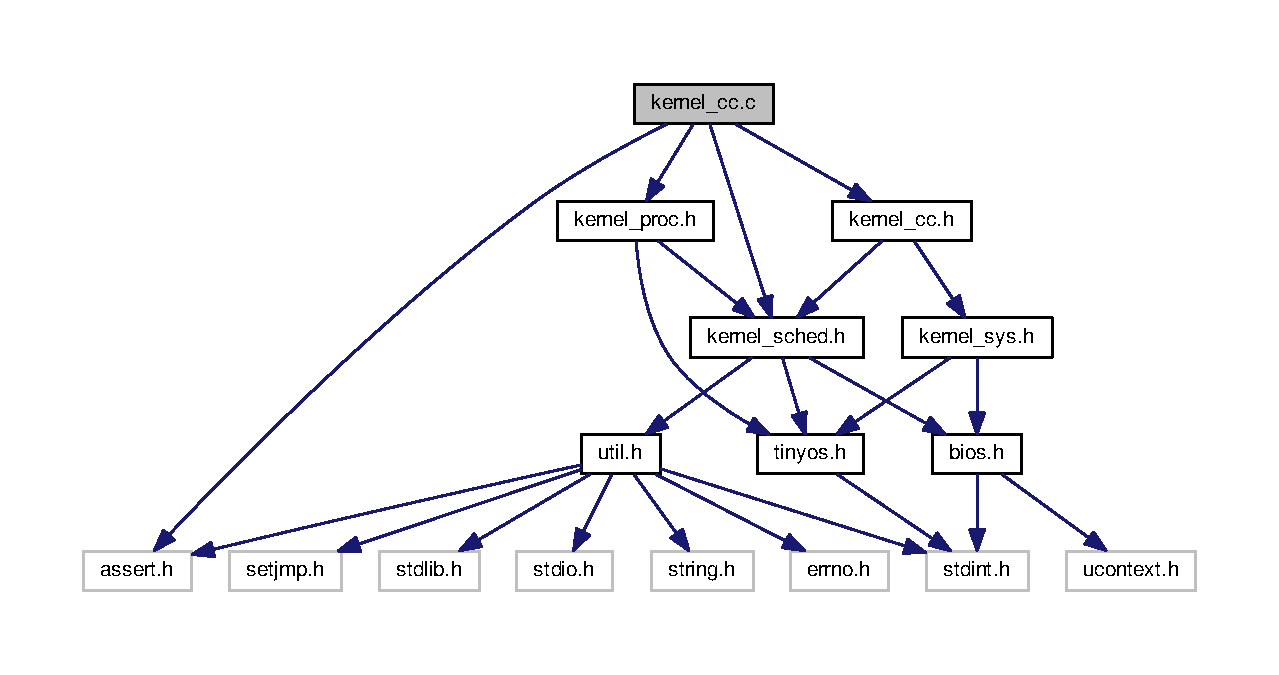
\includegraphics[width=350pt]{kernel__cc_8c__incl}
\end{center}
\end{figure}
\subsection*{Macros}
\begin{DoxyCompactItemize}
\item 
\#define {\bfseries M\+U\+T\+E\+X\+\_\+\+S\+P\+I\+NS}~1000\hypertarget{kernel__cc_8c_a146046d778f29cb1d176fcbd4d066733}{}\label{kernel__cc_8c_a146046d778f29cb1d176fcbd4d066733}

\end{DoxyCompactItemize}
\subsection*{Functions}
\begin{DoxyCompactItemize}
\item 
void \hyperlink{group__syscalls_ga1140be44df71d39edaf6a7262fb763ca}{Mutex\+\_\+\+Lock} (\hyperlink{group__syscalls_gaef2ec62cae8e0031fd19fc8b91083ade}{Mutex} $\ast$lock)
\begin{DoxyCompactList}\small\item\em Lock a mutex. \end{DoxyCompactList}\item 
void \hyperlink{group__syscalls_ga0b98d0315d0931d0c28104c36dd559c9}{Mutex\+\_\+\+Unlock} (\hyperlink{group__syscalls_gaef2ec62cae8e0031fd19fc8b91083ade}{Mutex} $\ast$lock)
\begin{DoxyCompactList}\small\item\em Unlock a mutex that you locked. \end{DoxyCompactList}\item 
static void {\bfseries remove\+\_\+from\+\_\+ring} (\hyperlink{structCondVar}{Cond\+Var} $\ast$cv, \+\_\+\+\_\+cv\+\_\+waiter $\ast$w)\hypertarget{kernel__cc_8c_abc2cf733db2b12d13a3f6e258f89dd2b}{}\label{kernel__cc_8c_abc2cf733db2b12d13a3f6e258f89dd2b}

\item 
static int {\bfseries cv\+\_\+wait} (\hyperlink{group__syscalls_gaef2ec62cae8e0031fd19fc8b91083ade}{Mutex} $\ast$mutex, \hyperlink{structCondVar}{Cond\+Var} $\ast$cv, enum \hyperlink{group__scheduler_gaad787d8d80312ffca3c0f197b3a25fbe}{S\+C\+H\+E\+D\+\_\+\+C\+A\+U\+SE} cause, \hyperlink{bios_8h_ae7291e5cd742fb9bc6d4aaa0d51bd0ee}{Timer\+Duration} timeout)\hypertarget{kernel__cc_8c_a639afd8d38fd525e27bf8bb1fadf24ee}{}\label{kernel__cc_8c_a639afd8d38fd525e27bf8bb1fadf24ee}

\item 
static void {\bfseries cv\+\_\+signal} (\hyperlink{structCondVar}{Cond\+Var} $\ast$cv)\hypertarget{kernel__cc_8c_a57708cb3ca29d1a575df0af638ca7d8d}{}\label{kernel__cc_8c_a57708cb3ca29d1a575df0af638ca7d8d}

\item 
int \hyperlink{group__syscalls_ga970dca2210b3f2ec8aedab7f542a9bf4}{Cond\+\_\+\+Wait} (\hyperlink{group__syscalls_gaef2ec62cae8e0031fd19fc8b91083ade}{Mutex} $\ast$mutex, \hyperlink{structCondVar}{Cond\+Var} $\ast$cv)
\begin{DoxyCompactList}\small\item\em Wait on a condition variable. \end{DoxyCompactList}\item 
int \hyperlink{group__syscalls_ga4e955b769339be9ea6a0c1bd4151c48f}{Cond\+\_\+\+Timed\+Wait} (\hyperlink{group__syscalls_gaef2ec62cae8e0031fd19fc8b91083ade}{Mutex} $\ast$mutex, \hyperlink{structCondVar}{Cond\+Var} $\ast$cv, \hyperlink{group__syscalls_gaf412159e5cef839836a5e7b19ee75d1c}{timeout\+\_\+t} timeout)
\begin{DoxyCompactList}\small\item\em Wait on a condition variable. \end{DoxyCompactList}\item 
void \hyperlink{group__syscalls_ga43f64f8be273d2fe77d7de5f4b81e22d}{Cond\+\_\+\+Signal} (\hyperlink{structCondVar}{Cond\+Var} $\ast$cv)
\begin{DoxyCompactList}\small\item\em Signal a condition variable. \end{DoxyCompactList}\item 
void \hyperlink{group__syscalls_ga8196aa2a48cad90742f254cc3b8fd351}{Cond\+\_\+\+Broadcast} (\hyperlink{structCondVar}{Cond\+Var} $\ast$cv)
\begin{DoxyCompactList}\small\item\em Notify all threads waiting at a condition variable. \end{DoxyCompactList}\item 
int \hyperlink{kernel__cc_8c_a6121802a0b64aae83288f60bf8a76834}{set\+\_\+core\+\_\+preemption} (int preempt)
\begin{DoxyCompactList}\small\item\em Set the preemption status for the current thread. \end{DoxyCompactList}\item 
int \hyperlink{kernel__cc_8c_ac3fd575c0f82fd75f8e7305be1107e2c}{get\+\_\+core\+\_\+preemption} ()
\begin{DoxyCompactList}\small\item\em Get the current preemption status. \end{DoxyCompactList}\item 
void \hyperlink{kernel__cc_8c_a64cbb83e8857ffaf703722363ac94f05}{kernel\+\_\+lock} ()\hypertarget{kernel__cc_8c_a64cbb83e8857ffaf703722363ac94f05}{}\label{kernel__cc_8c_a64cbb83e8857ffaf703722363ac94f05}

\begin{DoxyCompactList}\small\item\em Lock the kernel. \end{DoxyCompactList}\item 
void \hyperlink{kernel__cc_8c_a8ca062a9a1c570f34398bd177cb96e58}{kernel\+\_\+unlock} ()\hypertarget{kernel__cc_8c_a8ca062a9a1c570f34398bd177cb96e58}{}\label{kernel__cc_8c_a8ca062a9a1c570f34398bd177cb96e58}

\begin{DoxyCompactList}\small\item\em Unlock the kernel. \end{DoxyCompactList}\item 
int \hyperlink{kernel__cc_8c_a1fad5a21e5010939e1e0ad711192bc6c}{kernel\+\_\+wait\+\_\+wchan} (\hyperlink{structCondVar}{Cond\+Var} $\ast$cv, enum \hyperlink{group__scheduler_gaad787d8d80312ffca3c0f197b3a25fbe}{S\+C\+H\+E\+D\+\_\+\+C\+A\+U\+SE} cause, const char $\ast$wchan\+\_\+name, \hyperlink{bios_8h_ae7291e5cd742fb9bc6d4aaa0d51bd0ee}{Timer\+Duration} timeout)
\begin{DoxyCompactList}\small\item\em Wait on a condition variable using the kernel lock. \end{DoxyCompactList}\item 
void \hyperlink{kernel__cc_8c_a167cdb3f2a2285becf553405210eb08a}{kernel\+\_\+signal} (\hyperlink{structCondVar}{Cond\+Var} $\ast$cv)
\begin{DoxyCompactList}\small\item\em Signal a kernel condition to one waiter. \end{DoxyCompactList}\item 
void \hyperlink{kernel__cc_8c_a6ab8c1febc779de0c176d4e8a101ec5b}{kernel\+\_\+broadcast} (\hyperlink{structCondVar}{Cond\+Var} $\ast$cv)\hypertarget{kernel__cc_8c_a6ab8c1febc779de0c176d4e8a101ec5b}{}\label{kernel__cc_8c_a6ab8c1febc779de0c176d4e8a101ec5b}

\begin{DoxyCompactList}\small\item\em Signal a kernel condition to all waiters. \end{DoxyCompactList}\item 
void \hyperlink{kernel__cc_8c_aeafd158aa175ab53b85bc55dc4bbd962}{kernel\+\_\+sleep} (\hyperlink{group__scheduler_ga6c969c169777f82c104cf73e501df70f}{Thread\+\_\+state} newstate, enum \hyperlink{group__scheduler_gaad787d8d80312ffca3c0f197b3a25fbe}{S\+C\+H\+E\+D\+\_\+\+C\+A\+U\+SE} cause)
\begin{DoxyCompactList}\small\item\em Put thread to sleep, unlocking the kernel. \end{DoxyCompactList}\end{DoxyCompactItemize}
\subsection*{Variables}
\begin{DoxyCompactItemize}
\item 
\hyperlink{group__syscalls_gaef2ec62cae8e0031fd19fc8b91083ade}{Mutex} \hyperlink{kernel__cc_8c_a57ffb2dcd44b56da47dc03b2f85d9480}{kernel\+\_\+mutex} = \hyperlink{group__syscalls_ga96be0bfc33e7e113099c7546798bec99}{M\+U\+T\+E\+X\+\_\+\+I\+N\+IT}
\begin{DoxyCompactList}\small\item\em The kernel lock. \end{DoxyCompactList}\item 
static int {\bfseries kernel\+\_\+sem} = 1\hypertarget{kernel__cc_8c_a1c9aaa217ee98e133a7d199b5e0049f3}{}\label{kernel__cc_8c_a1c9aaa217ee98e133a7d199b5e0049f3}

\item 
static \hyperlink{structCondVar}{Cond\+Var} {\bfseries kernel\+\_\+sem\+\_\+cv} = \hyperlink{group__syscalls_ga6a7055a466bff255172e05f6ec82d792}{C\+O\+N\+D\+\_\+\+I\+N\+IT}\hypertarget{kernel__cc_8c_addaf45de2e9f92b9eb5ed68cc1017e6f}{}\label{kernel__cc_8c_addaf45de2e9f92b9eb5ed68cc1017e6f}

\end{DoxyCompactItemize}


\subsection{Detailed Description}
The implementation for concurrency control . 

Locks for scheduler and device drivers. Because we support multiple cores, we need to avoid race conditions with an interrupt handler on the same core, and also to avoid race conditions between cores. 

\subsection{Function Documentation}
\index{kernel\+\_\+cc.\+c@{kernel\+\_\+cc.\+c}!get\+\_\+core\+\_\+preemption@{get\+\_\+core\+\_\+preemption}}
\index{get\+\_\+core\+\_\+preemption@{get\+\_\+core\+\_\+preemption}!kernel\+\_\+cc.\+c@{kernel\+\_\+cc.\+c}}
\subsubsection[{\texorpdfstring{get\+\_\+core\+\_\+preemption()}{get_core_preemption()}}]{\setlength{\rightskip}{0pt plus 5cm}int get\+\_\+core\+\_\+preemption (
\begin{DoxyParamCaption}
{}
\end{DoxyParamCaption}
)}\hypertarget{kernel__cc_8c_ac3fd575c0f82fd75f8e7305be1107e2c}{}\label{kernel__cc_8c_ac3fd575c0f82fd75f8e7305be1107e2c}


Get the current preemption status. 

\begin{DoxyReturn}{Returns}
the current preemption status for this core, 0 means no preemption and 1 means preemption. 
\end{DoxyReturn}
\begin{DoxySeeAlso}{See also}
\hyperlink{kernel__cc_8h_a6121802a0b64aae83288f60bf8a76834}{set\+\_\+core\+\_\+preemption} 
\end{DoxySeeAlso}


Definition at line 243 of file kernel\+\_\+cc.\+c.

\index{kernel\+\_\+cc.\+c@{kernel\+\_\+cc.\+c}!kernel\+\_\+signal@{kernel\+\_\+signal}}
\index{kernel\+\_\+signal@{kernel\+\_\+signal}!kernel\+\_\+cc.\+c@{kernel\+\_\+cc.\+c}}
\subsubsection[{\texorpdfstring{kernel\+\_\+signal(\+Cond\+Var $\ast$cv)}{kernel_signal(CondVar *cv)}}]{\setlength{\rightskip}{0pt plus 5cm}void kernel\+\_\+signal (
\begin{DoxyParamCaption}
\item[{{\bf Cond\+Var} $\ast$}]{cv}
\end{DoxyParamCaption}
)}\hypertarget{kernel__cc_8c_a167cdb3f2a2285becf553405210eb08a}{}\label{kernel__cc_8c_a167cdb3f2a2285becf553405210eb08a}


Signal a kernel condition to one waiter. 

This call must be made 

Definition at line 324 of file kernel\+\_\+cc.\+c.

\index{kernel\+\_\+cc.\+c@{kernel\+\_\+cc.\+c}!kernel\+\_\+sleep@{kernel\+\_\+sleep}}
\index{kernel\+\_\+sleep@{kernel\+\_\+sleep}!kernel\+\_\+cc.\+c@{kernel\+\_\+cc.\+c}}
\subsubsection[{\texorpdfstring{kernel\+\_\+sleep(\+Thread\+\_\+state newstate, enum S\+C\+H\+E\+D\+\_\+\+C\+A\+U\+S\+E cause)}{kernel_sleep(Thread_state newstate, enum SCHED_CAUSE cause)}}]{\setlength{\rightskip}{0pt plus 5cm}void kernel\+\_\+sleep (
\begin{DoxyParamCaption}
\item[{{\bf Thread\+\_\+state}}]{state, }
\item[{enum {\bf S\+C\+H\+E\+D\+\_\+\+C\+A\+U\+SE}}]{cause}
\end{DoxyParamCaption}
)}\hypertarget{kernel__cc_8c_aeafd158aa175ab53b85bc55dc4bbd962}{}\label{kernel__cc_8c_aeafd158aa175ab53b85bc55dc4bbd962}


Put thread to sleep, unlocking the kernel. 

System calls should call this function instead of {\ttfamily sleep\+\_\+releasing}, as the kernel lock is not a mutex. 

Definition at line 334 of file kernel\+\_\+cc.\+c.

\index{kernel\+\_\+cc.\+c@{kernel\+\_\+cc.\+c}!kernel\+\_\+wait\+\_\+wchan@{kernel\+\_\+wait\+\_\+wchan}}
\index{kernel\+\_\+wait\+\_\+wchan@{kernel\+\_\+wait\+\_\+wchan}!kernel\+\_\+cc.\+c@{kernel\+\_\+cc.\+c}}
\subsubsection[{\texorpdfstring{kernel\+\_\+wait\+\_\+wchan(\+Cond\+Var $\ast$cv, enum S\+C\+H\+E\+D\+\_\+\+C\+A\+U\+S\+E cause, const char $\ast$wchan\+\_\+name, Timer\+Duration timeout)}{kernel_wait_wchan(CondVar *cv, enum SCHED_CAUSE cause, const char *wchan_name, TimerDuration timeout)}}]{\setlength{\rightskip}{0pt plus 5cm}int kernel\+\_\+wait\+\_\+wchan (
\begin{DoxyParamCaption}
\item[{{\bf Cond\+Var} $\ast$}]{cv, }
\item[{enum {\bf S\+C\+H\+E\+D\+\_\+\+C\+A\+U\+SE}}]{cause, }
\item[{const char $\ast$}]{wchan, }
\item[{{\bf Timer\+Duration}}]{timeout}
\end{DoxyParamCaption}
)}\hypertarget{kernel__cc_8c_a1fad5a21e5010939e1e0ad711192bc6c}{}\label{kernel__cc_8c_a1fad5a21e5010939e1e0ad711192bc6c}


Wait on a condition variable using the kernel lock. 

\begin{DoxyReturn}{Returns}
1 if signalled, 0 if not 
\end{DoxyReturn}


Definition at line 305 of file kernel\+\_\+cc.\+c.

\index{kernel\+\_\+cc.\+c@{kernel\+\_\+cc.\+c}!set\+\_\+core\+\_\+preemption@{set\+\_\+core\+\_\+preemption}}
\index{set\+\_\+core\+\_\+preemption@{set\+\_\+core\+\_\+preemption}!kernel\+\_\+cc.\+c@{kernel\+\_\+cc.\+c}}
\subsubsection[{\texorpdfstring{set\+\_\+core\+\_\+preemption(int preempt)}{set_core_preemption(int preempt)}}]{\setlength{\rightskip}{0pt plus 5cm}int set\+\_\+core\+\_\+preemption (
\begin{DoxyParamCaption}
\item[{int}]{preempt}
\end{DoxyParamCaption}
)}\hypertarget{kernel__cc_8c_a6121802a0b64aae83288f60bf8a76834}{}\label{kernel__cc_8c_a6121802a0b64aae83288f60bf8a76834}


Set the preemption status for the current thread. 

Depending on the value of the argument, this function will set preemption on or off. Preemption is disabled by disabling interrupts. This function is usually called via the convenience macros {\ttfamily preempt\+\_\+on} and {\ttfamily preempt\+\_\+off}. A typical non-\/preemptive section is declared as 
\begin{DoxyCode}
1 int preempt = preempt\_off;
2 ..
3     // do stuff without preemption 
4 ...
5 if(preempt) preempt\_on;
\end{DoxyCode}



\begin{DoxyParams}{Parameters}
{\em preempt} & the new preemption status \\
\hline
\end{DoxyParams}
\begin{DoxyReturn}{Returns}
the previous preemption status, where 0 means that preemption was previously off, and 1 means that it was on.
\end{DoxyReturn}
\begin{DoxySeeAlso}{See also}
\hyperlink{kernel__cc_8h_af936bcf607a61848cfea21c119f30905}{preempt\+\_\+off} 

\hyperlink{kernel__cc_8h_ac8efed506a60c7c6f02514e878a4004b}{preempt\+\_\+on} 
\end{DoxySeeAlso}


Definition at line 227 of file kernel\+\_\+cc.\+c.



\subsection{Variable Documentation}
\index{kernel\+\_\+cc.\+c@{kernel\+\_\+cc.\+c}!kernel\+\_\+mutex@{kernel\+\_\+mutex}}
\index{kernel\+\_\+mutex@{kernel\+\_\+mutex}!kernel\+\_\+cc.\+c@{kernel\+\_\+cc.\+c}}
\subsubsection[{\texorpdfstring{kernel\+\_\+mutex}{kernel_mutex}}]{\setlength{\rightskip}{0pt plus 5cm}{\bf Mutex} kernel\+\_\+mutex = {\bf M\+U\+T\+E\+X\+\_\+\+I\+N\+IT}}\hypertarget{kernel__cc_8c_a57ffb2dcd44b56da47dc03b2f85d9480}{}\label{kernel__cc_8c_a57ffb2dcd44b56da47dc03b2f85d9480}


The kernel lock. 

Kernel locking is provided by a semaphore, implemented as a monitor. A semaphre for kernel locking has the advantage that ????????????? 

Definition at line 265 of file kernel\+\_\+cc.\+c.


\hypertarget{kernel__cc_8h}{}\section{kernel\+\_\+cc.\+h File Reference}
\label{kernel__cc_8h}\index{kernel\+\_\+cc.\+h@{kernel\+\_\+cc.\+h}}


Concurrency and preemption control A\+PI.  


{\ttfamily \#include \char`\"{}kernel\+\_\+sys.\+h\char`\"{}}\\*
{\ttfamily \#include \char`\"{}kernel\+\_\+sched.\+h\char`\"{}}\\*
Include dependency graph for kernel\+\_\+cc.\+h\+:\nopagebreak
\begin{figure}[H]
\begin{center}
\leavevmode
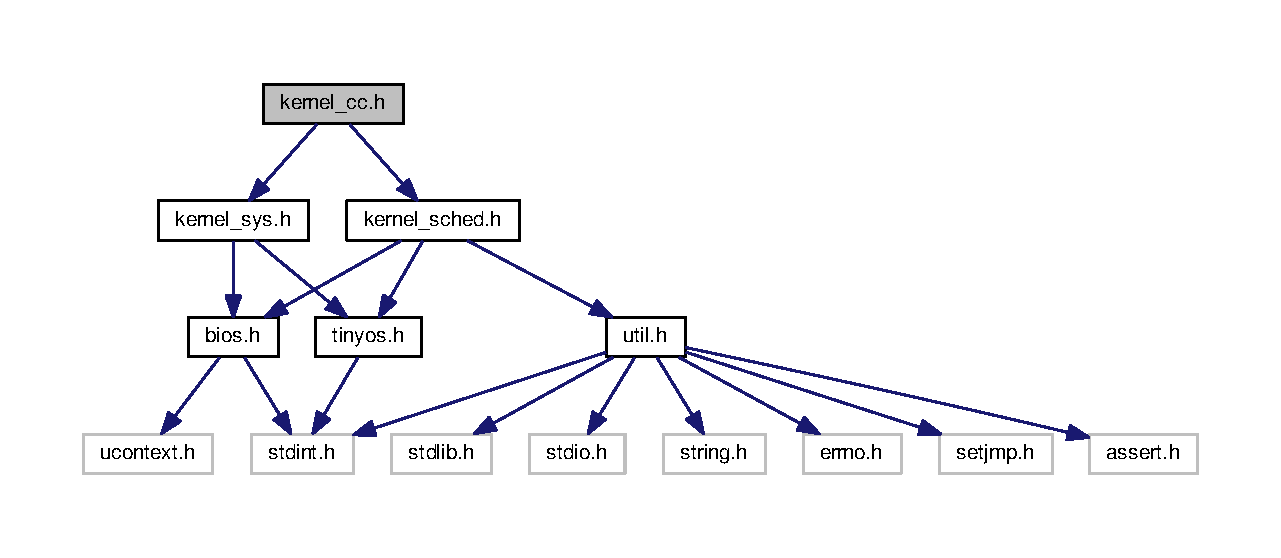
\includegraphics[width=350pt]{kernel__cc_8h__incl}
\end{center}
\end{figure}
This graph shows which files directly or indirectly include this file\+:\nopagebreak
\begin{figure}[H]
\begin{center}
\leavevmode
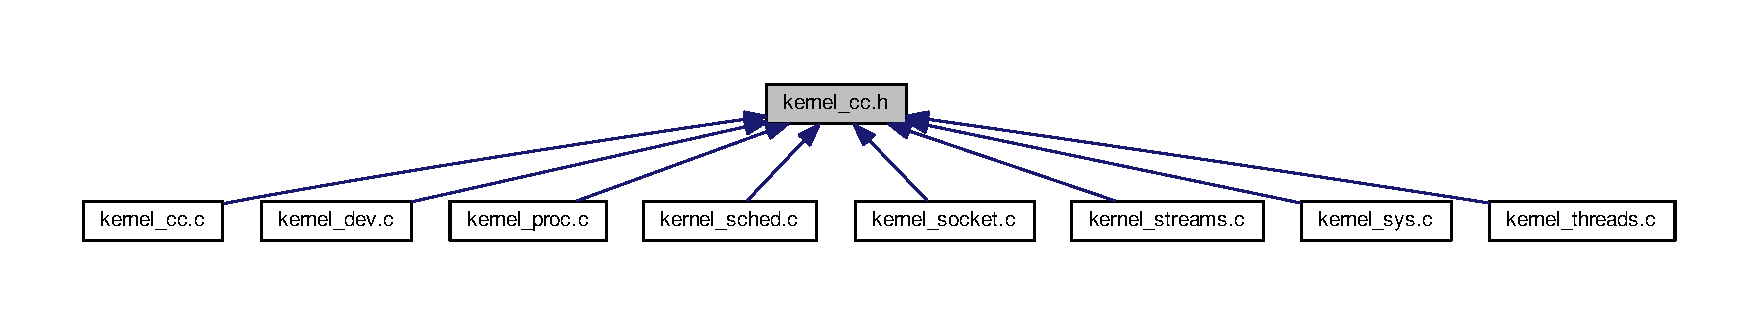
\includegraphics[width=350pt]{kernel__cc_8h__dep__incl}
\end{center}
\end{figure}
\subsection*{Macros}
\begin{DoxyCompactItemize}
\item 
\#define {\bfseries kernel\+\_\+wait}(cv,  cause)~\hyperlink{kernel__cc_8h_abe7f999775e4f5a56201bf88a9eeb2a1}{kernel\+\_\+wait\+\_\+wchan}((cv),(cause),\+\_\+\+\_\+\+F\+U\+N\+C\+T\+I\+O\+N\+\_\+\+\_\+, \hyperlink{group__scheduler_ga462fb2ba6f2af99ec3d021ded436bb65}{N\+O\+\_\+\+T\+I\+M\+E\+O\+UT})\hypertarget{kernel__cc_8h_a327d5485981b426c5e7079387dd3073b}{}\label{kernel__cc_8h_a327d5485981b426c5e7079387dd3073b}

\item 
\#define {\bfseries kernel\+\_\+timedwait}(cv,  cause,  timeout)~\hyperlink{kernel__cc_8h_abe7f999775e4f5a56201bf88a9eeb2a1}{kernel\+\_\+wait\+\_\+wchan}((cv),(cause),\+\_\+\+\_\+\+F\+U\+N\+C\+T\+I\+O\+N\+\_\+\+\_\+, (timeout))\hypertarget{kernel__cc_8h_ada476fc3746c5de3a120ff33b26e3c13}{}\label{kernel__cc_8h_ada476fc3746c5de3a120ff33b26e3c13}

\item 
\#define \hyperlink{kernel__cc_8h_af936bcf607a61848cfea21c119f30905}{preempt\+\_\+off}~(\hyperlink{kernel__cc_8h_a6121802a0b64aae83288f60bf8a76834}{set\+\_\+core\+\_\+preemption}(0))
\begin{DoxyCompactList}\small\item\em Easily turn preemption off. \end{DoxyCompactList}\item 
\#define \hyperlink{kernel__cc_8h_ac8efed506a60c7c6f02514e878a4004b}{preempt\+\_\+on}~(\hyperlink{kernel__cc_8h_a6121802a0b64aae83288f60bf8a76834}{set\+\_\+core\+\_\+preemption}(1))
\begin{DoxyCompactList}\small\item\em Easily turn preemption off. \end{DoxyCompactList}\end{DoxyCompactItemize}
\subsection*{Functions}
\begin{DoxyCompactItemize}
\item 
void \hyperlink{kernel__cc_8h_a64cbb83e8857ffaf703722363ac94f05}{kernel\+\_\+lock} ()\hypertarget{kernel__cc_8h_a64cbb83e8857ffaf703722363ac94f05}{}\label{kernel__cc_8h_a64cbb83e8857ffaf703722363ac94f05}

\begin{DoxyCompactList}\small\item\em Lock the kernel. \end{DoxyCompactList}\item 
void \hyperlink{kernel__cc_8h_a8ca062a9a1c570f34398bd177cb96e58}{kernel\+\_\+unlock} ()\hypertarget{kernel__cc_8h_a8ca062a9a1c570f34398bd177cb96e58}{}\label{kernel__cc_8h_a8ca062a9a1c570f34398bd177cb96e58}

\begin{DoxyCompactList}\small\item\em Unlock the kernel. \end{DoxyCompactList}\item 
int \hyperlink{kernel__cc_8h_abe7f999775e4f5a56201bf88a9eeb2a1}{kernel\+\_\+wait\+\_\+wchan} (\hyperlink{structCondVar}{Cond\+Var} $\ast$cv, enum \hyperlink{group__scheduler_gaad787d8d80312ffca3c0f197b3a25fbe}{S\+C\+H\+E\+D\+\_\+\+C\+A\+U\+SE} cause, const char $\ast$wchan, \hyperlink{bios_8h_ae7291e5cd742fb9bc6d4aaa0d51bd0ee}{Timer\+Duration} timeout)
\begin{DoxyCompactList}\small\item\em Wait on a condition variable using the kernel lock. \end{DoxyCompactList}\item 
void \hyperlink{kernel__cc_8h_a167cdb3f2a2285becf553405210eb08a}{kernel\+\_\+signal} (\hyperlink{structCondVar}{Cond\+Var} $\ast$cv)
\begin{DoxyCompactList}\small\item\em Signal a kernel condition to one waiter. \end{DoxyCompactList}\item 
void \hyperlink{kernel__cc_8h_a6ab8c1febc779de0c176d4e8a101ec5b}{kernel\+\_\+broadcast} (\hyperlink{structCondVar}{Cond\+Var} $\ast$cv)\hypertarget{kernel__cc_8h_a6ab8c1febc779de0c176d4e8a101ec5b}{}\label{kernel__cc_8h_a6ab8c1febc779de0c176d4e8a101ec5b}

\begin{DoxyCompactList}\small\item\em Signal a kernel condition to all waiters. \end{DoxyCompactList}\item 
void \hyperlink{kernel__cc_8h_ac108cbd1eb069858a5ed9e576069c464}{kernel\+\_\+sleep} (\hyperlink{group__scheduler_ga6c969c169777f82c104cf73e501df70f}{Thread\+\_\+state} state, enum \hyperlink{group__scheduler_gaad787d8d80312ffca3c0f197b3a25fbe}{S\+C\+H\+E\+D\+\_\+\+C\+A\+U\+SE} cause)
\begin{DoxyCompactList}\small\item\em Put thread to sleep, unlocking the kernel. \end{DoxyCompactList}\item 
int \hyperlink{kernel__cc_8h_a6121802a0b64aae83288f60bf8a76834}{set\+\_\+core\+\_\+preemption} (int preempt)
\begin{DoxyCompactList}\small\item\em Set the preemption status for the current thread. \end{DoxyCompactList}\item 
int \hyperlink{kernel__cc_8h_ac3fd575c0f82fd75f8e7305be1107e2c}{get\+\_\+core\+\_\+preemption} ()
\begin{DoxyCompactList}\small\item\em Get the current preemption status. \end{DoxyCompactList}\end{DoxyCompactItemize}
\subsection*{Variables}
\begin{DoxyCompactItemize}
\item 
\hyperlink{group__syscalls_gaef2ec62cae8e0031fd19fc8b91083ade}{Mutex} \hyperlink{kernel__cc_8h_a57ffb2dcd44b56da47dc03b2f85d9480}{kernel\+\_\+mutex}
\begin{DoxyCompactList}\small\item\em The kernel lock. \end{DoxyCompactList}\end{DoxyCompactItemize}


\subsection{Detailed Description}
Concurrency and preemption control A\+PI. 



\subsection{Macro Definition Documentation}
\index{kernel\+\_\+cc.\+h@{kernel\+\_\+cc.\+h}!preempt\+\_\+off@{preempt\+\_\+off}}
\index{preempt\+\_\+off@{preempt\+\_\+off}!kernel\+\_\+cc.\+h@{kernel\+\_\+cc.\+h}}
\subsubsection[{\texorpdfstring{preempt\+\_\+off}{preempt_off}}]{\setlength{\rightskip}{0pt plus 5cm}\#define preempt\+\_\+off~({\bf set\+\_\+core\+\_\+preemption}(0))}\hypertarget{kernel__cc_8h_af936bcf607a61848cfea21c119f30905}{}\label{kernel__cc_8h_af936bcf607a61848cfea21c119f30905}


Easily turn preemption off. 

\begin{DoxySeeAlso}{See also}
\hyperlink{kernel__cc_8h_a6121802a0b64aae83288f60bf8a76834}{set\+\_\+core\+\_\+preemption} 
\end{DoxySeeAlso}


Definition at line 121 of file kernel\+\_\+cc.\+h.

\index{kernel\+\_\+cc.\+h@{kernel\+\_\+cc.\+h}!preempt\+\_\+on@{preempt\+\_\+on}}
\index{preempt\+\_\+on@{preempt\+\_\+on}!kernel\+\_\+cc.\+h@{kernel\+\_\+cc.\+h}}
\subsubsection[{\texorpdfstring{preempt\+\_\+on}{preempt_on}}]{\setlength{\rightskip}{0pt plus 5cm}\#define preempt\+\_\+on~({\bf set\+\_\+core\+\_\+preemption}(1))}\hypertarget{kernel__cc_8h_ac8efed506a60c7c6f02514e878a4004b}{}\label{kernel__cc_8h_ac8efed506a60c7c6f02514e878a4004b}


Easily turn preemption off. 

\begin{DoxySeeAlso}{See also}
\hyperlink{kernel__cc_8h_a6121802a0b64aae83288f60bf8a76834}{set\+\_\+core\+\_\+preemption} 
\end{DoxySeeAlso}


Definition at line 126 of file kernel\+\_\+cc.\+h.



\subsection{Function Documentation}
\index{kernel\+\_\+cc.\+h@{kernel\+\_\+cc.\+h}!get\+\_\+core\+\_\+preemption@{get\+\_\+core\+\_\+preemption}}
\index{get\+\_\+core\+\_\+preemption@{get\+\_\+core\+\_\+preemption}!kernel\+\_\+cc.\+h@{kernel\+\_\+cc.\+h}}
\subsubsection[{\texorpdfstring{get\+\_\+core\+\_\+preemption()}{get_core_preemption()}}]{\setlength{\rightskip}{0pt plus 5cm}int get\+\_\+core\+\_\+preemption (
\begin{DoxyParamCaption}
{}
\end{DoxyParamCaption}
)}\hypertarget{kernel__cc_8h_ac3fd575c0f82fd75f8e7305be1107e2c}{}\label{kernel__cc_8h_ac3fd575c0f82fd75f8e7305be1107e2c}


Get the current preemption status. 

\begin{DoxyReturn}{Returns}
the current preemption status for this core, 0 means no preemption and 1 means preemption. 
\end{DoxyReturn}
\begin{DoxySeeAlso}{See also}
\hyperlink{kernel__cc_8h_a6121802a0b64aae83288f60bf8a76834}{set\+\_\+core\+\_\+preemption} 
\end{DoxySeeAlso}


Definition at line 243 of file kernel\+\_\+cc.\+c.

\index{kernel\+\_\+cc.\+h@{kernel\+\_\+cc.\+h}!kernel\+\_\+signal@{kernel\+\_\+signal}}
\index{kernel\+\_\+signal@{kernel\+\_\+signal}!kernel\+\_\+cc.\+h@{kernel\+\_\+cc.\+h}}
\subsubsection[{\texorpdfstring{kernel\+\_\+signal(\+Cond\+Var $\ast$cv)}{kernel_signal(CondVar *cv)}}]{\setlength{\rightskip}{0pt plus 5cm}void kernel\+\_\+signal (
\begin{DoxyParamCaption}
\item[{{\bf Cond\+Var} $\ast$}]{cv}
\end{DoxyParamCaption}
)}\hypertarget{kernel__cc_8h_a167cdb3f2a2285becf553405210eb08a}{}\label{kernel__cc_8h_a167cdb3f2a2285becf553405210eb08a}


Signal a kernel condition to one waiter. 

This call must be made 

Definition at line 324 of file kernel\+\_\+cc.\+c.

\index{kernel\+\_\+cc.\+h@{kernel\+\_\+cc.\+h}!kernel\+\_\+sleep@{kernel\+\_\+sleep}}
\index{kernel\+\_\+sleep@{kernel\+\_\+sleep}!kernel\+\_\+cc.\+h@{kernel\+\_\+cc.\+h}}
\subsubsection[{\texorpdfstring{kernel\+\_\+sleep(\+Thread\+\_\+state state, enum S\+C\+H\+E\+D\+\_\+\+C\+A\+U\+S\+E cause)}{kernel_sleep(Thread_state state, enum SCHED_CAUSE cause)}}]{\setlength{\rightskip}{0pt plus 5cm}void kernel\+\_\+sleep (
\begin{DoxyParamCaption}
\item[{{\bf Thread\+\_\+state}}]{state, }
\item[{enum {\bf S\+C\+H\+E\+D\+\_\+\+C\+A\+U\+SE}}]{cause}
\end{DoxyParamCaption}
)}\hypertarget{kernel__cc_8h_ac108cbd1eb069858a5ed9e576069c464}{}\label{kernel__cc_8h_ac108cbd1eb069858a5ed9e576069c464}


Put thread to sleep, unlocking the kernel. 

System calls should call this function instead of {\ttfamily sleep\+\_\+releasing}, as the kernel lock is not a mutex. 

Definition at line 334 of file kernel\+\_\+cc.\+c.

\index{kernel\+\_\+cc.\+h@{kernel\+\_\+cc.\+h}!kernel\+\_\+wait\+\_\+wchan@{kernel\+\_\+wait\+\_\+wchan}}
\index{kernel\+\_\+wait\+\_\+wchan@{kernel\+\_\+wait\+\_\+wchan}!kernel\+\_\+cc.\+h@{kernel\+\_\+cc.\+h}}
\subsubsection[{\texorpdfstring{kernel\+\_\+wait\+\_\+wchan(\+Cond\+Var $\ast$cv, enum S\+C\+H\+E\+D\+\_\+\+C\+A\+U\+S\+E cause, const char $\ast$wchan, Timer\+Duration timeout)}{kernel_wait_wchan(CondVar *cv, enum SCHED_CAUSE cause, const char *wchan, TimerDuration timeout)}}]{\setlength{\rightskip}{0pt plus 5cm}int kernel\+\_\+wait\+\_\+wchan (
\begin{DoxyParamCaption}
\item[{{\bf Cond\+Var} $\ast$}]{cv, }
\item[{enum {\bf S\+C\+H\+E\+D\+\_\+\+C\+A\+U\+SE}}]{cause, }
\item[{const char $\ast$}]{wchan, }
\item[{{\bf Timer\+Duration}}]{timeout}
\end{DoxyParamCaption}
)}\hypertarget{kernel__cc_8h_abe7f999775e4f5a56201bf88a9eeb2a1}{}\label{kernel__cc_8h_abe7f999775e4f5a56201bf88a9eeb2a1}


Wait on a condition variable using the kernel lock. 

\begin{DoxyReturn}{Returns}
1 if signalled, 0 if not 
\end{DoxyReturn}


Definition at line 305 of file kernel\+\_\+cc.\+c.

\index{kernel\+\_\+cc.\+h@{kernel\+\_\+cc.\+h}!set\+\_\+core\+\_\+preemption@{set\+\_\+core\+\_\+preemption}}
\index{set\+\_\+core\+\_\+preemption@{set\+\_\+core\+\_\+preemption}!kernel\+\_\+cc.\+h@{kernel\+\_\+cc.\+h}}
\subsubsection[{\texorpdfstring{set\+\_\+core\+\_\+preemption(int preempt)}{set_core_preemption(int preempt)}}]{\setlength{\rightskip}{0pt plus 5cm}int set\+\_\+core\+\_\+preemption (
\begin{DoxyParamCaption}
\item[{int}]{preempt}
\end{DoxyParamCaption}
)}\hypertarget{kernel__cc_8h_a6121802a0b64aae83288f60bf8a76834}{}\label{kernel__cc_8h_a6121802a0b64aae83288f60bf8a76834}


Set the preemption status for the current thread. 

Depending on the value of the argument, this function will set preemption on or off. Preemption is disabled by disabling interrupts. This function is usually called via the convenience macros {\ttfamily preempt\+\_\+on} and {\ttfamily preempt\+\_\+off}. A typical non-\/preemptive section is declared as 
\begin{DoxyCode}
1 int preempt = preempt\_off;
2 ..
3     // do stuff without preemption 
4 ...
5 if(preempt) preempt\_on;
\end{DoxyCode}



\begin{DoxyParams}{Parameters}
{\em preempt} & the new preemption status \\
\hline
\end{DoxyParams}
\begin{DoxyReturn}{Returns}
the previous preemption status, where 0 means that preemption was previously off, and 1 means that it was on.
\end{DoxyReturn}
\begin{DoxySeeAlso}{See also}
\hyperlink{kernel__cc_8h_af936bcf607a61848cfea21c119f30905}{preempt\+\_\+off} 

\hyperlink{kernel__cc_8h_ac8efed506a60c7c6f02514e878a4004b}{preempt\+\_\+on} 
\end{DoxySeeAlso}


Definition at line 227 of file kernel\+\_\+cc.\+c.



\subsection{Variable Documentation}
\index{kernel\+\_\+cc.\+h@{kernel\+\_\+cc.\+h}!kernel\+\_\+mutex@{kernel\+\_\+mutex}}
\index{kernel\+\_\+mutex@{kernel\+\_\+mutex}!kernel\+\_\+cc.\+h@{kernel\+\_\+cc.\+h}}
\subsubsection[{\texorpdfstring{kernel\+\_\+mutex}{kernel_mutex}}]{\setlength{\rightskip}{0pt plus 5cm}{\bf Mutex} kernel\+\_\+mutex}\hypertarget{kernel__cc_8h_a57ffb2dcd44b56da47dc03b2f85d9480}{}\label{kernel__cc_8h_a57ffb2dcd44b56da47dc03b2f85d9480}


The kernel lock. 

Kernel locking is provided by a semaphore, implemented as a monitor. A semaphre for kernel locking has the advantage that ????????????? 

Definition at line 265 of file kernel\+\_\+cc.\+c.


\hypertarget{kernel__dev_8h}{}\section{kernel\+\_\+dev.\+h File Reference}
\label{kernel__dev_8h}\index{kernel\+\_\+dev.\+h@{kernel\+\_\+dev.\+h}}


Device management.  


{\ttfamily \#include \char`\"{}util.\+h\char`\"{}}\\*
{\ttfamily \#include \char`\"{}bios.\+h\char`\"{}}\\*
Include dependency graph for kernel\+\_\+dev.\+h\+:\nopagebreak
\begin{figure}[H]
\begin{center}
\leavevmode
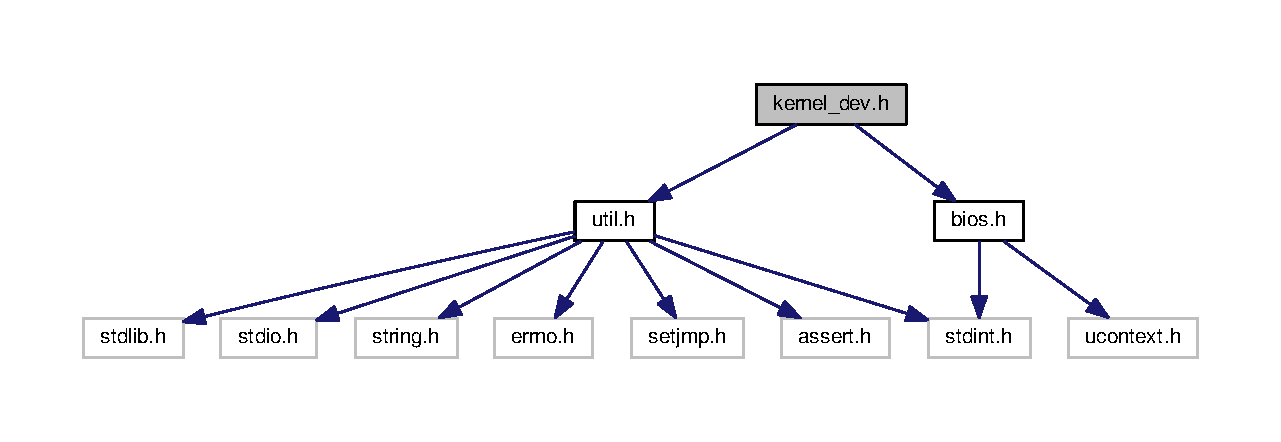
\includegraphics[width=350pt]{kernel__dev_8h__incl}
\end{center}
\end{figure}
This graph shows which files directly or indirectly include this file\+:\nopagebreak
\begin{figure}[H]
\begin{center}
\leavevmode
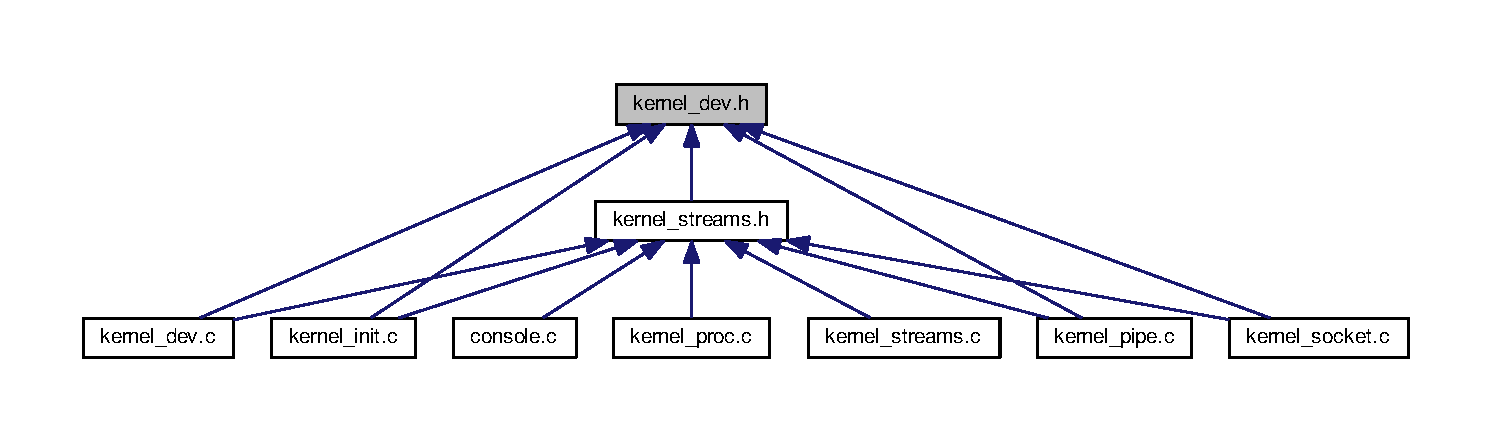
\includegraphics[width=350pt]{kernel__dev_8h__dep__incl}
\end{center}
\end{figure}
\subsection*{Data Structures}
\begin{DoxyCompactItemize}
\item 
struct \hyperlink{structfile__operations}{file\+\_\+operations}
\begin{DoxyCompactList}\small\item\em The device-\/specific file operations table. \end{DoxyCompactList}\item 
struct \hyperlink{structdevice__control__block}{device\+\_\+control\+\_\+block}
\begin{DoxyCompactList}\small\item\em Device control block. \end{DoxyCompactList}\end{DoxyCompactItemize}
\subsection*{Typedefs}
\begin{DoxyCompactItemize}
\item 
typedef struct \hyperlink{structfile__operations}{file\+\_\+operations} \hyperlink{group__dev_gaab625d8ae3a95e942ed10ed1579f5042}{file\+\_\+ops}
\begin{DoxyCompactList}\small\item\em The device-\/specific file operations table. \end{DoxyCompactList}\item 
typedef struct \hyperlink{structdevice__control__block}{device\+\_\+control\+\_\+block} \hyperlink{group__dev_gaf0e2d4a982667466d84f6fb7522611d6}{D\+CB}
\begin{DoxyCompactList}\small\item\em Device control block. \end{DoxyCompactList}\end{DoxyCompactItemize}
\subsection*{Enumerations}
\begin{DoxyCompactItemize}
\item 
enum \hyperlink{group__dev_ga879ceac20e83b2375e5b49f4379b0c90}{Device\+\_\+type} \{ \hyperlink{group__dev_gga879ceac20e83b2375e5b49f4379b0c90a8ca9ed7c2fc080b6706582ccf828b08f}{D\+E\+V\+\_\+\+N\+U\+LL}, 
\hyperlink{group__dev_gga879ceac20e83b2375e5b49f4379b0c90adb43c91cf279ccd4510abaed9425bacc}{D\+E\+V\+\_\+\+S\+E\+R\+I\+AL}, 
\hyperlink{group__dev_gga879ceac20e83b2375e5b49f4379b0c90a4d07dfbc7e68d26e2d92773a37381ce7}{D\+E\+V\+\_\+\+M\+AX}
 \}\begin{DoxyCompactList}\small\item\em The device type. \end{DoxyCompactList}
\end{DoxyCompactItemize}
\subsection*{Functions}
\begin{DoxyCompactItemize}
\item 
void \hyperlink{group__dev_ga840b5c2460abea4a19a201f7d6d035c8}{initialize\+\_\+devices} ()
\begin{DoxyCompactList}\small\item\em Initialization for devices. \end{DoxyCompactList}\item 
int \hyperlink{group__dev_ga6d8e08550640c9819aa07b6bba9fa6ed}{device\+\_\+open} (\hyperlink{group__dev_ga879ceac20e83b2375e5b49f4379b0c90}{Device\+\_\+type} major, \hyperlink{bios_8h_a91ad9478d81a7aaf2593e8d9c3d06a14}{uint} minor, void $\ast$$\ast$obj, \hyperlink{group__dev_gaab625d8ae3a95e942ed10ed1579f5042}{file\+\_\+ops} $\ast$$\ast$ops)
\begin{DoxyCompactList}\small\item\em Open a device. \end{DoxyCompactList}\item 
\hyperlink{bios_8h_a91ad9478d81a7aaf2593e8d9c3d06a14}{uint} \hyperlink{group__dev_ga0808cf584a510e0eff6908a5313ce296}{device\+\_\+no} (\hyperlink{group__dev_ga879ceac20e83b2375e5b49f4379b0c90}{Device\+\_\+type} major)
\begin{DoxyCompactList}\small\item\em Get the number of devices of a particular major number. \end{DoxyCompactList}\end{DoxyCompactItemize}


\subsection{Detailed Description}
Device management. 


\hypertarget{kernel__proc_8h}{}\section{kernel\+\_\+proc.\+h File Reference}
\label{kernel__proc_8h}\index{kernel\+\_\+proc.\+h@{kernel\+\_\+proc.\+h}}


The process table and process management.  


{\ttfamily \#include \char`\"{}tinyos.\+h\char`\"{}}\\*
{\ttfamily \#include \char`\"{}kernel\+\_\+sched.\+h\char`\"{}}\\*
Include dependency graph for kernel\+\_\+proc.\+h\+:\nopagebreak
\begin{figure}[H]
\begin{center}
\leavevmode
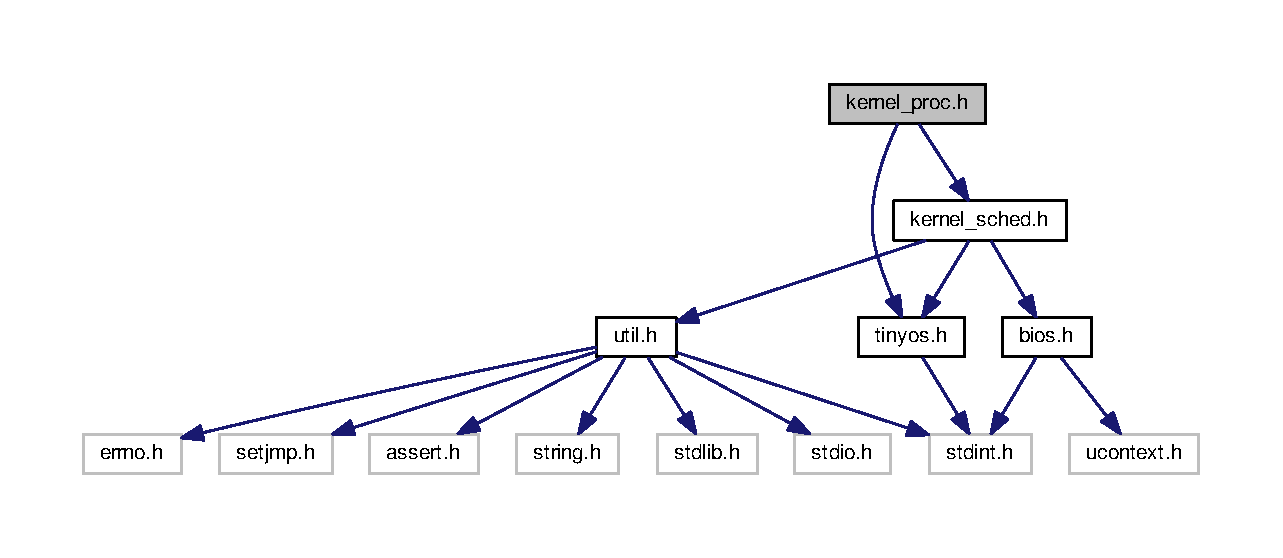
\includegraphics[width=350pt]{kernel__proc_8h__incl}
\end{center}
\end{figure}
This graph shows which files directly or indirectly include this file\+:\nopagebreak
\begin{figure}[H]
\begin{center}
\leavevmode
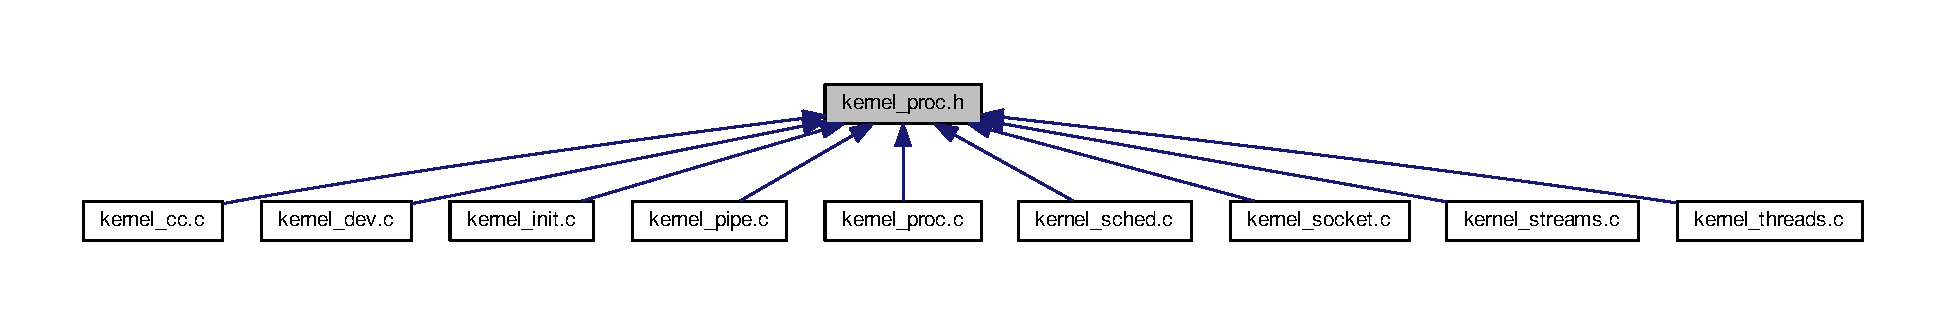
\includegraphics[width=350pt]{kernel__proc_8h__dep__incl}
\end{center}
\end{figure}
\subsection*{Data Structures}
\begin{DoxyCompactItemize}
\item 
struct \hyperlink{structprocess__control__block}{process\+\_\+control\+\_\+block}
\begin{DoxyCompactList}\small\item\em Process Control Block. \end{DoxyCompactList}\item 
struct \hyperlink{structprocess__thread__control__block}{process\+\_\+thread\+\_\+control\+\_\+block}
\end{DoxyCompactItemize}
\subsection*{Typedefs}
\begin{DoxyCompactItemize}
\item 
typedef enum \hyperlink{group__proc_ga4f133ac5f9b2ca9c1446889baee1dc05}{pid\+\_\+state\+\_\+e} \hyperlink{group__proc_gade1eea4d20492c4c97263201145e5097}{pid\+\_\+state}
\begin{DoxyCompactList}\small\item\em P\+ID state. \end{DoxyCompactList}\item 
typedef struct \hyperlink{structprocess__control__block}{process\+\_\+control\+\_\+block} \hyperlink{group__proc_ga91aaadf0c3f9cef2293a99c69795323f}{P\+CB}
\begin{DoxyCompactList}\small\item\em Process Control Block. \end{DoxyCompactList}\item 
typedef struct \hyperlink{structprocess__thread__control__block}{process\+\_\+thread\+\_\+control\+\_\+block} {\bfseries P\+T\+CB}
\end{DoxyCompactItemize}
\subsection*{Enumerations}
\begin{DoxyCompactItemize}
\item 
enum \hyperlink{group__proc_ga4f133ac5f9b2ca9c1446889baee1dc05}{pid\+\_\+state\+\_\+e} \{ \hyperlink{group__proc_gga4f133ac5f9b2ca9c1446889baee1dc05acc62d1576546f3245237e1b232d838b6}{F\+R\+EE}, 
\hyperlink{group__proc_gga4f133ac5f9b2ca9c1446889baee1dc05a4f34c5c191d6e0d028ca831b6c0b1571}{A\+L\+I\+VE}, 
\hyperlink{group__proc_gga4f133ac5f9b2ca9c1446889baee1dc05a5dfb36109b24f39d54d5c3f48f53def8}{Z\+O\+M\+B\+IE}
 \}\begin{DoxyCompactList}\small\item\em P\+ID state. \end{DoxyCompactList}
\end{DoxyCompactItemize}
\subsection*{Functions}
\begin{DoxyCompactItemize}
\item 
void \hyperlink{group__proc_ga82948cbeb57bb0b6e15d1f14f06a2db3}{initialize\+\_\+processes} ()
\begin{DoxyCompactList}\small\item\em Initialize the process table. \end{DoxyCompactList}\item 
\hyperlink{group__proc_ga91aaadf0c3f9cef2293a99c69795323f}{P\+CB} $\ast$ \hyperlink{group__proc_ga10cf45ea8bc92b00bd1f25553b9cf5c8}{get\+\_\+pcb} (\hyperlink{group__syscalls_gafac07f3170763932fac97b6eab2c3984}{Pid\+\_\+t} pid)
\begin{DoxyCompactList}\small\item\em Get the P\+CB for a P\+ID. \end{DoxyCompactList}\item 
\hyperlink{group__syscalls_gafac07f3170763932fac97b6eab2c3984}{Pid\+\_\+t} \hyperlink{group__proc_ga110e884cb053244b18d1058751a78cfe}{get\+\_\+pid} (\hyperlink{group__proc_ga91aaadf0c3f9cef2293a99c69795323f}{P\+CB} $\ast$pcb)
\begin{DoxyCompactList}\small\item\em Get the P\+ID of a P\+CB. \end{DoxyCompactList}\end{DoxyCompactItemize}


\subsection{Detailed Description}
The process table and process management. 


\hypertarget{kernel__sched_8h}{}\section{kernel\+\_\+sched.\+h File Reference}
\label{kernel__sched_8h}\index{kernel\+\_\+sched.\+h@{kernel\+\_\+sched.\+h}}


Tiny\+OS kernel\+: The Scheduler A\+PI.  


{\ttfamily \#include \char`\"{}util.\+h\char`\"{}}\\*
{\ttfamily \#include \char`\"{}bios.\+h\char`\"{}}\\*
{\ttfamily \#include \char`\"{}tinyos.\+h\char`\"{}}\\*
Include dependency graph for kernel\+\_\+sched.\+h\+:\nopagebreak
\begin{figure}[H]
\begin{center}
\leavevmode
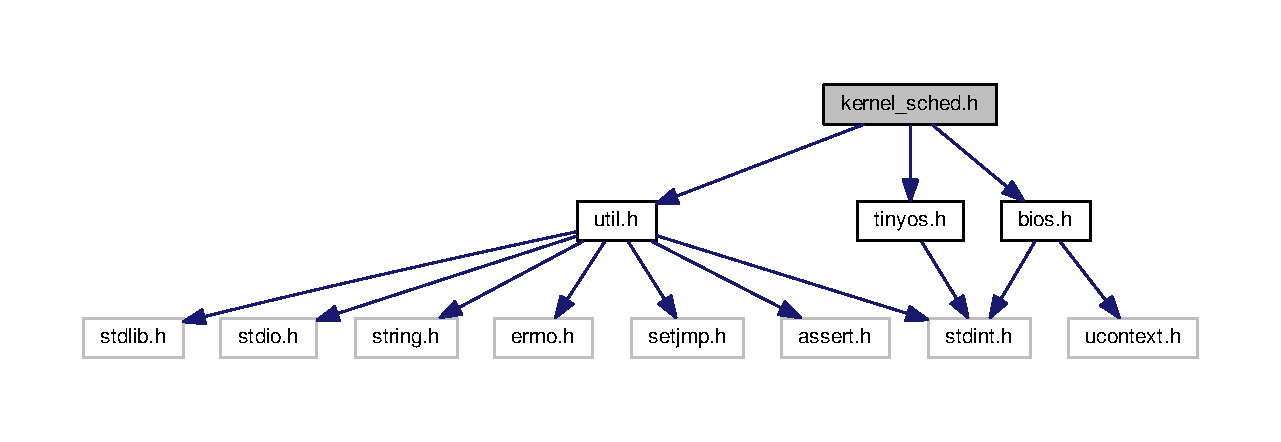
\includegraphics[width=350pt]{kernel__sched_8h__incl}
\end{center}
\end{figure}
This graph shows which files directly or indirectly include this file\+:\nopagebreak
\begin{figure}[H]
\begin{center}
\leavevmode
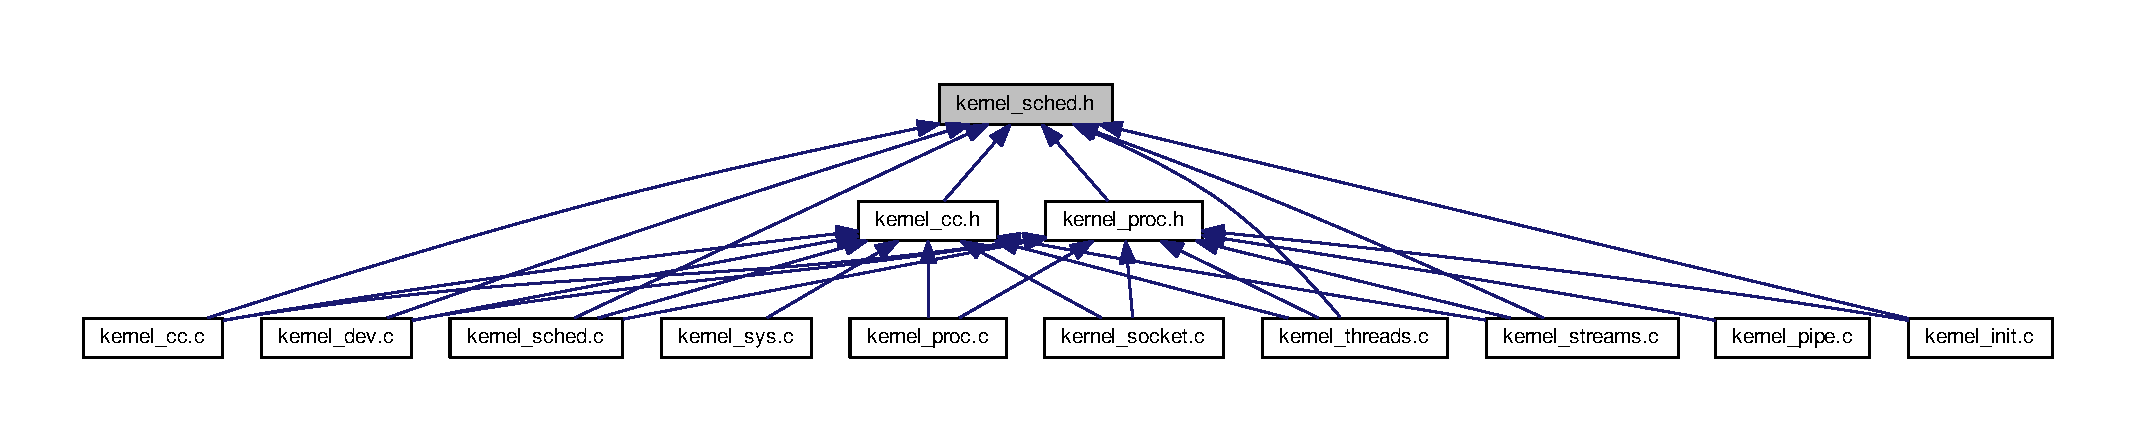
\includegraphics[width=350pt]{kernel__sched_8h__dep__incl}
\end{center}
\end{figure}
\subsection*{Data Structures}
\begin{DoxyCompactItemize}
\item 
struct \hyperlink{structthread__control__block}{thread\+\_\+control\+\_\+block}
\begin{DoxyCompactList}\small\item\em The thread control block. \end{DoxyCompactList}\item 
struct \hyperlink{structcore__control__block}{core\+\_\+control\+\_\+block}
\begin{DoxyCompactList}\small\item\em Core control block. \end{DoxyCompactList}\end{DoxyCompactItemize}
\subsection*{Macros}
\begin{DoxyCompactItemize}
\item 
\#define {\bfseries M\+A\+X\+\_\+\+P\+R\+I\+O\+R\+I\+T\+Y\+\_\+\+S\+T\+AY}~100
\item 
\#define \hyperlink{group__scheduler_ga90b7a8cb7bc3fdbd98014a3e15ee6e9a}{T\+H\+R\+E\+A\+D\+\_\+\+S\+T\+A\+C\+K\+\_\+\+S\+I\+ZE}~(128$\ast$1024)
\item 
\#define \hyperlink{group__scheduler_ga869aabe01f7b28027376354dd895b96b}{C\+U\+R\+C\+O\+RE}~(\hyperlink{group__scheduler_ga3be3b151b275926dff3fb99bee765eab}{cctx}\mbox{[}\hyperlink{bios_8h_abac58ced7d51f54f2318b326bc991933}{cpu\+\_\+core\+\_\+id}\mbox{]})
\begin{DoxyCompactList}\small\item\em The current core\textquotesingle{}s C\+CB. \end{DoxyCompactList}\item 
\#define \hyperlink{group__scheduler_ga587a82c8931f0df72f43cc913ceb7e27}{C\+U\+R\+T\+H\+R\+E\+AD}~(C\+U\+R\+C\+O\+R\+E.\+current\+\_\+thread)
\begin{DoxyCompactList}\small\item\em The current thread. \end{DoxyCompactList}\item 
\#define \hyperlink{group__scheduler_gae3437e8e6787ef05b6576d03c5b6a0ca}{C\+U\+R\+P\+R\+OC}~(\hyperlink{group__scheduler_ga587a82c8931f0df72f43cc913ceb7e27}{C\+U\+R\+T\+H\+R\+E\+AD}-\/$>$owner\+\_\+pcb)
\begin{DoxyCompactList}\small\item\em The current thread. \end{DoxyCompactList}\item 
\#define \hyperlink{group__scheduler_ga462fb2ba6f2af99ec3d021ded436bb65}{N\+O\+\_\+\+T\+I\+M\+E\+O\+UT}~((\hyperlink{bios_8h_ae7291e5cd742fb9bc6d4aaa0d51bd0ee}{Timer\+Duration})-\/1)
\begin{DoxyCompactList}\small\item\em A timeout constant, denoting no timeout for sleep. \end{DoxyCompactList}\item 
\#define \hyperlink{group__scheduler_gabc4f0f9abea1b5443308e4ea84b52b21}{Q\+U\+A\+N\+T\+UM}~(10000\+L)
\begin{DoxyCompactList}\small\item\em Quantum (in microseconds) \end{DoxyCompactList}\end{DoxyCompactItemize}
\subsection*{Typedefs}
\begin{DoxyCompactItemize}
\item 
typedef struct \hyperlink{structthread__control__block}{thread\+\_\+control\+\_\+block} \hyperlink{group__scheduler_gaf88d9c946bf70b36a1e8bc34383abfc9}{T\+CB}
\begin{DoxyCompactList}\small\item\em The thread control block. \end{DoxyCompactList}\item 
typedef struct \hyperlink{structcore__control__block}{core\+\_\+control\+\_\+block} \hyperlink{group__scheduler_ga7485b31e0dd9fd723bc2d75fba5206a0}{C\+CB}
\begin{DoxyCompactList}\small\item\em Core control block. \end{DoxyCompactList}\end{DoxyCompactItemize}
\subsection*{Enumerations}
\begin{DoxyCompactItemize}
\item 
enum \hyperlink{group__scheduler_ga6c969c169777f82c104cf73e501df70f}{Thread\+\_\+state} \{ \\*
\hyperlink{group__scheduler_gga6c969c169777f82c104cf73e501df70fa0cb1b2c6a7db1f1084886c98909a3f36}{I\+N\+IT}, 
\hyperlink{group__scheduler_gga6c969c169777f82c104cf73e501df70fa6564f2f3e15be06b670547bbcaaf0798}{R\+E\+A\+DY}, 
\hyperlink{group__scheduler_gga6c969c169777f82c104cf73e501df70fa1061be6c3fb88d32829cba6f6b2be304}{R\+U\+N\+N\+I\+NG}, 
\hyperlink{group__scheduler_gga6c969c169777f82c104cf73e501df70fa948b2aee15f52b421fa4770c47bcfe8c}{S\+T\+O\+P\+P\+ED}, 
\\*
\hyperlink{group__scheduler_gga6c969c169777f82c104cf73e501df70fab9f9543350f6bd6191e52158daa88884}{E\+X\+I\+T\+ED}
 \}\begin{DoxyCompactList}\small\item\em Thread state. \end{DoxyCompactList}
\item 
enum \hyperlink{group__scheduler_gab180b4aa356776bddcd724cef4f5deae}{Thread\+\_\+phase} \{ \hyperlink{group__scheduler_ggab180b4aa356776bddcd724cef4f5deaeaa826daca588e692c88114586b0de472b}{C\+T\+X\+\_\+\+C\+L\+E\+AN}, 
\hyperlink{group__scheduler_ggab180b4aa356776bddcd724cef4f5deaea2b4b41fda67c1a83e6523675515c007b}{C\+T\+X\+\_\+\+D\+I\+R\+TY}
 \}\begin{DoxyCompactList}\small\item\em Thread phase. \end{DoxyCompactList}
\item 
enum \hyperlink{group__scheduler_ga18795bc1ab00161fc27ce34b1895fb03}{Thread\+\_\+type} \{ \hyperlink{group__scheduler_gga18795bc1ab00161fc27ce34b1895fb03abc11b4e4eba50c875d7ed6bc34090dd3}{I\+D\+L\+E\+\_\+\+T\+H\+R\+E\+AD}, 
\hyperlink{group__scheduler_gga18795bc1ab00161fc27ce34b1895fb03a1d3bb8be1deb6ac7be94fea88e1ed76b}{N\+O\+R\+M\+A\+L\+\_\+\+T\+H\+R\+E\+AD}
 \}\begin{DoxyCompactList}\small\item\em Thread type. \end{DoxyCompactList}
\item 
enum \hyperlink{group__scheduler_gaad787d8d80312ffca3c0f197b3a25fbe}{S\+C\+H\+E\+D\+\_\+\+C\+A\+U\+SE} \{ \\*
\hyperlink{group__scheduler_ggaad787d8d80312ffca3c0f197b3a25fbea99764e3e8f3195b33e888c816c9a0207}{S\+C\+H\+E\+D\+\_\+\+Q\+U\+A\+N\+T\+UM}, 
\hyperlink{group__scheduler_ggaad787d8d80312ffca3c0f197b3a25fbeaa19b25dfae8d75a5900bb23a1f6c64d8}{S\+C\+H\+E\+D\+\_\+\+IO}, 
\hyperlink{group__scheduler_ggaad787d8d80312ffca3c0f197b3a25fbea7d3764881e09d1f0dbf2d8ef09640a37}{S\+C\+H\+E\+D\+\_\+\+M\+U\+T\+EX}, 
\hyperlink{group__scheduler_ggaad787d8d80312ffca3c0f197b3a25fbea5f78cf7f43e406215d39f936fa99fd5a}{S\+C\+H\+E\+D\+\_\+\+P\+I\+PE}, 
\\*
\hyperlink{group__scheduler_ggaad787d8d80312ffca3c0f197b3a25fbea1b7d43bbe4e4eb4089beb28b2c8f7e50}{S\+C\+H\+E\+D\+\_\+\+P\+O\+LL}, 
\hyperlink{group__scheduler_ggaad787d8d80312ffca3c0f197b3a25fbea525b9af8477ce2505c0d559940d827e5}{S\+C\+H\+E\+D\+\_\+\+I\+D\+LE}, 
\hyperlink{group__scheduler_ggaad787d8d80312ffca3c0f197b3a25fbea9ead280a8852a73f1ba3368d66338275}{S\+C\+H\+E\+D\+\_\+\+U\+S\+ER}, 
\hyperlink{group__scheduler_ggaad787d8d80312ffca3c0f197b3a25fbeaa22d6ce0d6e60054464bc01e9b7a34d6}{S\+C\+H\+E\+D\+\_\+\+I\+N\+IT}
 \}\begin{DoxyCompactList}\small\item\em Designate different origins of scheduler invocation. \end{DoxyCompactList}
\end{DoxyCompactItemize}
\subsection*{Functions}
\begin{DoxyCompactItemize}
\item 
\hyperlink{group__scheduler_gaf88d9c946bf70b36a1e8bc34383abfc9}{T\+CB} $\ast$ \hyperlink{group__scheduler_gab0a2dca5105d7e856f03c0cc4dc4d707}{spawn\+\_\+thread} (\hyperlink{group__proc_ga91aaadf0c3f9cef2293a99c69795323f}{P\+CB} $\ast$pcb, void($\ast$func)(), \hyperlink{structprocess__thread__control__block}{P\+T\+CB} $\ast$ptcb)
\begin{DoxyCompactList}\small\item\em Create a new thread. \end{DoxyCompactList}\item 
int \hyperlink{group__scheduler_gae8301452fd9ae5bf7cd7f2676650ff06}{wakeup} (\hyperlink{group__scheduler_gaf88d9c946bf70b36a1e8bc34383abfc9}{T\+CB} $\ast$tcb)
\begin{DoxyCompactList}\small\item\em Wakeup a blocked thread. \end{DoxyCompactList}\item 
void \hyperlink{group__scheduler_ga0ab1a2dcfbfe3fb09cc24044efddfd34}{sleep\+\_\+releasing} (\hyperlink{group__scheduler_ga6c969c169777f82c104cf73e501df70f}{Thread\+\_\+state} newstate, \hyperlink{group__syscalls_gaef2ec62cae8e0031fd19fc8b91083ade}{Mutex} $\ast$mx, enum \hyperlink{group__scheduler_gaad787d8d80312ffca3c0f197b3a25fbe}{S\+C\+H\+E\+D\+\_\+\+C\+A\+U\+SE} cause, \hyperlink{bios_8h_ae7291e5cd742fb9bc6d4aaa0d51bd0ee}{Timer\+Duration} timeout)
\begin{DoxyCompactList}\small\item\em Block the current thread. \end{DoxyCompactList}\item 
void \hyperlink{group__scheduler_ga1db327892199949812ae5a52119f2e97}{yield} (enum \hyperlink{group__scheduler_gaad787d8d80312ffca3c0f197b3a25fbe}{S\+C\+H\+E\+D\+\_\+\+C\+A\+U\+SE} cause)
\begin{DoxyCompactList}\small\item\em Give up the C\+PU. \end{DoxyCompactList}\item 
void \hyperlink{group__scheduler_ga147600b59d656eb9d9558673c2fad36d}{run\+\_\+scheduler} (void)
\begin{DoxyCompactList}\small\item\em Enter the scheduler. \end{DoxyCompactList}\item 
void \hyperlink{group__scheduler_ga244fb594301322e79d11a7844c759bba}{initialize\+\_\+scheduler} (void)
\begin{DoxyCompactList}\small\item\em Initialize the scheduler. \end{DoxyCompactList}\end{DoxyCompactItemize}
\subsection*{Variables}
\begin{DoxyCompactItemize}
\item 
\hyperlink{group__scheduler_ga7485b31e0dd9fd723bc2d75fba5206a0}{C\+CB} \hyperlink{group__scheduler_ga3be3b151b275926dff3fb99bee765eab}{cctx} \mbox{[}\hyperlink{bios_8h_a009855593b59738d24dbfc236edb3b14}{M\+A\+X\+\_\+\+C\+O\+R\+ES}\mbox{]}
\begin{DoxyCompactList}\small\item\em the array of Core Control Blocks (C\+CB) for the kernel \end{DoxyCompactList}\end{DoxyCompactItemize}


\subsection{Detailed Description}
Tiny\+OS kernel\+: The Scheduler A\+PI. 


\hypertarget{kernel__streams_8h}{}\section{kernel\+\_\+streams.\+h File Reference}
\label{kernel__streams_8h}\index{kernel\+\_\+streams.\+h@{kernel\+\_\+streams.\+h}}


Support for I/O streams.  


{\ttfamily \#include \char`\"{}tinyos.\+h\char`\"{}}\\*
{\ttfamily \#include \char`\"{}kernel\+\_\+dev.\+h\char`\"{}}\\*
Include dependency graph for kernel\+\_\+streams.\+h\+:\nopagebreak
\begin{figure}[H]
\begin{center}
\leavevmode
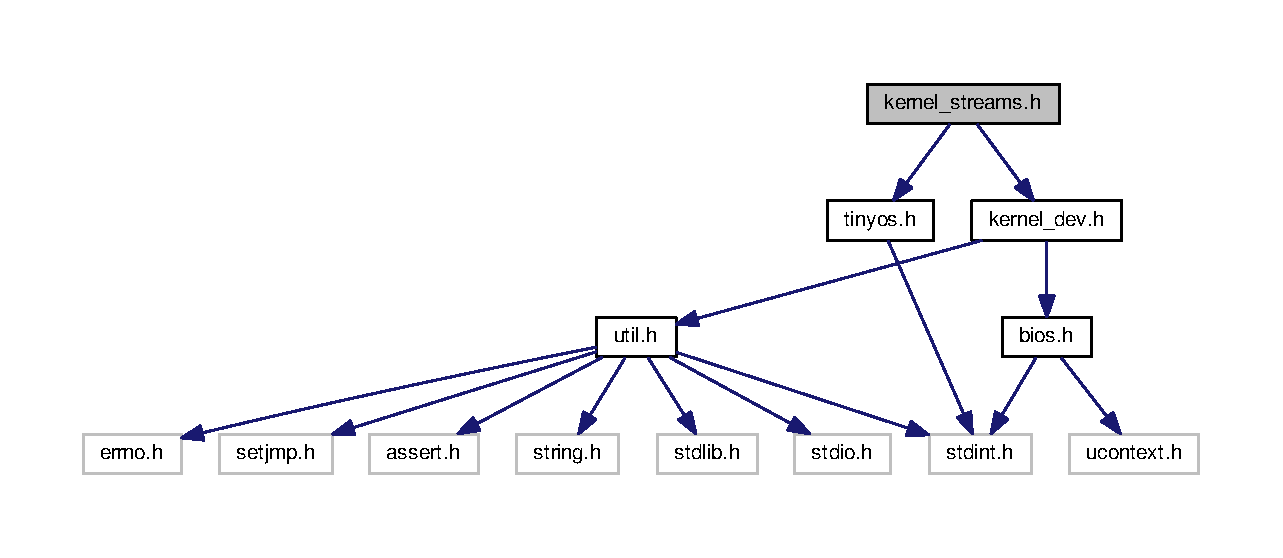
\includegraphics[width=350pt]{kernel__streams_8h__incl}
\end{center}
\end{figure}
This graph shows which files directly or indirectly include this file\+:\nopagebreak
\begin{figure}[H]
\begin{center}
\leavevmode
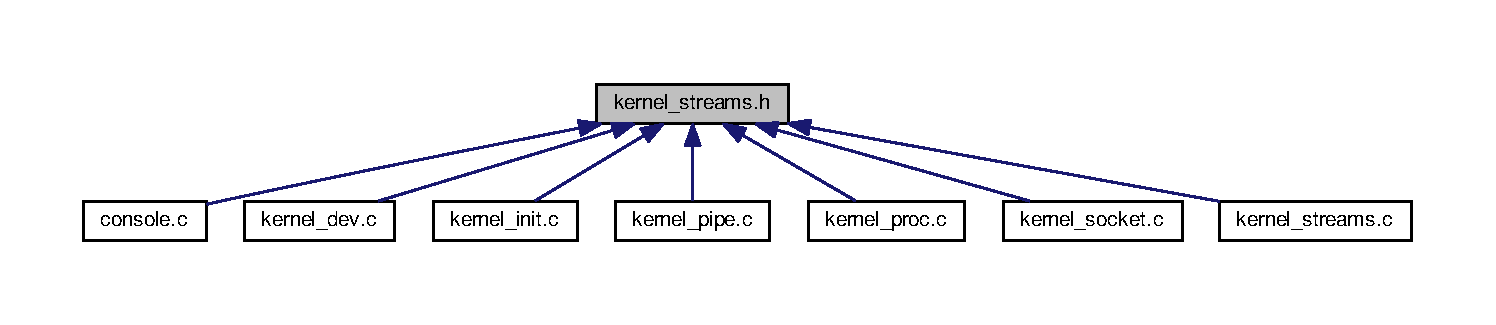
\includegraphics[width=350pt]{kernel__streams_8h__dep__incl}
\end{center}
\end{figure}
\subsection*{Data Structures}
\begin{DoxyCompactItemize}
\item 
struct \hyperlink{structfile__control__block}{file\+\_\+control\+\_\+block}
\begin{DoxyCompactList}\small\item\em The file control block. \end{DoxyCompactList}\item 
struct \hyperlink{structpipe__control__block}{pipe\+\_\+control\+\_\+block}
\end{DoxyCompactItemize}
\subsection*{Typedefs}
\begin{DoxyCompactItemize}
\item 
typedef struct \hyperlink{structfile__control__block}{file\+\_\+control\+\_\+block} \hyperlink{group__streams_ga0c7e751afb9d6cadebf070961804d400}{F\+CB}
\begin{DoxyCompactList}\small\item\em The file control block. \end{DoxyCompactList}\item 
typedef struct \hyperlink{structpipe__control__block}{pipe\+\_\+control\+\_\+block} {\bfseries P\+P\+CB}
\end{DoxyCompactItemize}
\subsection*{Functions}
\begin{DoxyCompactItemize}
\item 
void \hyperlink{group__streams_ga147537248d983b0cc6cc7e8b39245f09}{initialize\+\_\+files} ()
\begin{DoxyCompactList}\small\item\em Initialization for files and streams. \end{DoxyCompactList}\item 
void \hyperlink{group__streams_ga409efca0b415dfdabe868c292d1daf66}{F\+C\+B\+\_\+incref} (\hyperlink{group__streams_ga0c7e751afb9d6cadebf070961804d400}{F\+CB} $\ast$fcb)
\begin{DoxyCompactList}\small\item\em Increase the reference count of an fcb. \end{DoxyCompactList}\item 
int \hyperlink{group__streams_ga26586eafc28dd1f2ac5bc7402922aa36}{F\+C\+B\+\_\+decref} (\hyperlink{group__streams_ga0c7e751afb9d6cadebf070961804d400}{F\+CB} $\ast$fcb)
\begin{DoxyCompactList}\small\item\em Decrease the reference count of the fcb. \end{DoxyCompactList}\item 
int \hyperlink{group__streams_ga462269376de145171b87b7bc3036e4f8}{F\+C\+B\+\_\+reserve} (size\+\_\+t num, \hyperlink{group__syscalls_ga5097222c5f0da97d92d4712359abc38f}{Fid\+\_\+t} $\ast$fid, \hyperlink{group__streams_ga0c7e751afb9d6cadebf070961804d400}{F\+CB} $\ast$$\ast$fcb)
\begin{DoxyCompactList}\small\item\em Acquire a number of F\+C\+Bs and corresponding fids. \end{DoxyCompactList}\item 
void \hyperlink{group__streams_gac44c094845a8d4e2e13f9df5b17274df}{F\+C\+B\+\_\+unreserve} (size\+\_\+t num, \hyperlink{group__syscalls_ga5097222c5f0da97d92d4712359abc38f}{Fid\+\_\+t} $\ast$fid, \hyperlink{group__streams_ga0c7e751afb9d6cadebf070961804d400}{F\+CB} $\ast$$\ast$fcb)
\begin{DoxyCompactList}\small\item\em Release a number of F\+C\+Bs and corresponding fids. \end{DoxyCompactList}\item 
\hyperlink{group__streams_ga0c7e751afb9d6cadebf070961804d400}{F\+CB} $\ast$ \hyperlink{group__streams_ga36b4f172aba29ba2660d0aed0f10d60b}{get\+\_\+fcb} (\hyperlink{group__syscalls_ga5097222c5f0da97d92d4712359abc38f}{Fid\+\_\+t} fid)
\begin{DoxyCompactList}\small\item\em Translate an fid to an F\+CB. \end{DoxyCompactList}\item 
\hyperlink{structpipe__control__block}{P\+P\+CB} $\ast$ {\bfseries create\+Pipe} ()
\end{DoxyCompactItemize}
\subsection*{Variables}
\begin{DoxyCompactItemize}
\item 
static \hyperlink{group__dev_gaab625d8ae3a95e942ed10ed1579f5042}{file\+\_\+ops} {\bfseries writer\+\_\+ops}
\item 
static \hyperlink{group__dev_gaab625d8ae3a95e942ed10ed1579f5042}{file\+\_\+ops} {\bfseries reader\+\_\+ops}
\end{DoxyCompactItemize}


\subsection{Detailed Description}
Support for I/O streams. 


\hypertarget{symposium_8h}{}\section{symposium.\+h File Reference}
\label{symposium_8h}\index{symposium.\+h@{symposium.\+h}}


An implementation of Dining Philosophers.  


{\ttfamily \#include \char`\"{}tinyos.\+h\char`\"{}}\\*
Include dependency graph for symposium.\+h\+:\nopagebreak
\begin{figure}[H]
\begin{center}
\leavevmode
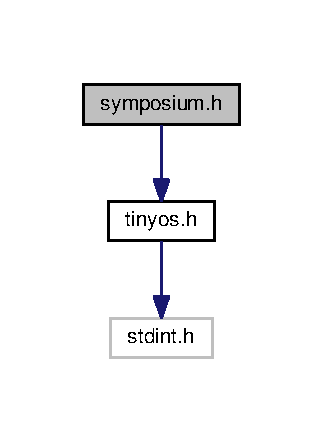
\includegraphics[width=155pt]{symposium_8h__incl}
\end{center}
\end{figure}
This graph shows which files directly or indirectly include this file\+:\nopagebreak
\begin{figure}[H]
\begin{center}
\leavevmode
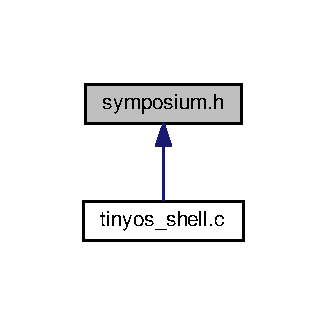
\includegraphics[width=157pt]{symposium_8h__dep__incl}
\end{center}
\end{figure}
\subsection*{Data Structures}
\begin{DoxyCompactItemize}
\item 
struct \hyperlink{structsymposium__t}{symposium\+\_\+t}
\begin{DoxyCompactList}\small\item\em A symposium definition. \end{DoxyCompactList}\item 
struct \hyperlink{structSymposiumTable}{Symposium\+Table}
\begin{DoxyCompactList}\small\item\em A symposium monitor. \end{DoxyCompactList}\end{DoxyCompactItemize}
\subsection*{Macros}
\begin{DoxyCompactItemize}
\item 
\#define \hyperlink{symposium_8h_aa8c7593792d981b932c6eb4a9188edff}{F\+B\+A\+SE}~35\hypertarget{symposium_8h_aa8c7593792d981b932c6eb4a9188edff}{}\label{symposium_8h_aa8c7593792d981b932c6eb4a9188edff}

\begin{DoxyCompactList}\small\item\em The default for constant $F_\text{BASE}$. \end{DoxyCompactList}\item 
\#define \hyperlink{symposium_8h_a2c3f0109071e4c85f626dab0a13dda90}{F\+G\+AP}~10\hypertarget{symposium_8h_a2c3f0109071e4c85f626dab0a13dda90}{}\label{symposium_8h_a2c3f0109071e4c85f626dab0a13dda90}

\begin{DoxyCompactList}\small\item\em The default for constant $F_\text{GAP}$. \end{DoxyCompactList}\end{DoxyCompactItemize}
\subsection*{Enumerations}
\begin{DoxyCompactItemize}
\item 
enum \hyperlink{symposium_8h_a9fced5fb7d50a8fa2e8ae45b0cae3520}{P\+H\+IL} \{ {\bfseries N\+O\+T\+H\+E\+RE} =0, 
{\bfseries T\+H\+I\+N\+K\+I\+NG}, 
{\bfseries H\+U\+N\+G\+RY}, 
{\bfseries E\+A\+T\+I\+NG}
 \}\hypertarget{symposium_8h_a9fced5fb7d50a8fa2e8ae45b0cae3520}{}\label{symposium_8h_a9fced5fb7d50a8fa2e8ae45b0cae3520}
\begin{DoxyCompactList}\small\item\em A philosopher\textquotesingle{}s state. \end{DoxyCompactList}
\end{DoxyCompactItemize}
\subsection*{Functions}
\begin{DoxyCompactItemize}
\item 
unsigned int \hyperlink{symposium_8h_a84513d2aec8501a26825e23f0e450ca5}{fibo} (unsigned int n)
\begin{DoxyCompactList}\small\item\em Compute the n-\/th Fibonacci number recursively. \end{DoxyCompactList}\item 
void \hyperlink{symposium_8h_a900dd2c0958369a94ba06efb7a352216}{adjust\+\_\+symposium} (\hyperlink{structsymposium__t}{symposium\+\_\+t} $\ast$table, int d\+B\+A\+SE, int d\+G\+AP)
\begin{DoxyCompactList}\small\item\em Adjust a symposium\textquotesingle{}s duration. \end{DoxyCompactList}\item 
void \hyperlink{symposium_8h_acee238ec1bec29869630d48b21c54904}{Symposium\+Table\+\_\+init} (\hyperlink{structSymposiumTable}{Symposium\+Table} $\ast$table, \hyperlink{structsymposium__t}{symposium\+\_\+t} $\ast$symp)
\begin{DoxyCompactList}\small\item\em Initialize a symposium monitor. \end{DoxyCompactList}\item 
void \hyperlink{symposium_8h_af52cdc1038db2959d8af09fa5f13032f}{Symposium\+Table\+\_\+destroy} (\hyperlink{structSymposiumTable}{Symposium\+Table} $\ast$table)
\begin{DoxyCompactList}\small\item\em Destroy a symposium monitor. \end{DoxyCompactList}\item 
void \hyperlink{symposium_8h_ad0a96304b18eeb599ee43e14ed1c2e56}{Symposium\+Table\+\_\+philosopher} (\hyperlink{structSymposiumTable}{Symposium\+Table} $\ast$table, int i)
\begin{DoxyCompactList}\small\item\em The philosopher. \end{DoxyCompactList}\item 
int \hyperlink{symposium_8h_a5214bc7f5ae83c1db2e14b40dea86948}{Symposium\+Of\+Threads} (int argl, void $\ast$args)
\begin{DoxyCompactList}\small\item\em Run a symposium using threads. \end{DoxyCompactList}\item 
int \hyperlink{symposium_8h_a528034fb39aa477a05b57211c9614ebe}{Symposium\+Of\+Processes} (int argl, void $\ast$args)
\begin{DoxyCompactList}\small\item\em Run a symposium using processes. \end{DoxyCompactList}\end{DoxyCompactItemize}


\subsection{Detailed Description}
An implementation of Dining Philosophers. 

The Dining Philisophers are sitting around a Symposium roundtable. Each philosopher comes to the table, cycles between thinking and eating a number of times, and leaves the table. However,
\begin{DoxyItemize}
\item in order to eat she needs to hold a fork in each hand, and
\item there is only one fork between two philosophers. Therefore, a philosopher may wait hungry for forks to become available.
\end{DoxyItemize}

In our simulation, a philosopher is a thread. The symposium is implemented as a monitor, with each philosopher waiting at their own condition variable.

During each thinking or eating period, a philosopher computes Fibonacci numbers using an exponentially expensive recursion\+: \[ F(n+2) = F(n+1) + F(n) \] with $F(0) = 0$ and $F(1)=1$. The complexity of this recursion is $ O( \phi^n )$ where $\phi=\frac{1+\sqrt{5}}{2}\approx 1.618$ is the {\bfseries golden ratio}.

For each thinking session, an integer $n$ is drawn uniformly at random from the set $ [f_\text{min}, f_\text{max}] $.

Overall, a symposium is specified by four numbers\+:
\begin{DoxyItemize}
\item {\ttfamily N}, the number of philosophers
\item {\ttfamily bites}, the number of times each of them eats
\item $f_\text{min}, f_\text{max}$ which determine the time of each thinking and eating period.
\end{DoxyItemize}

In order to make symposia with a large number of philosophers or number of bites, we can compute suitable values of $f_\text{min}, f_\text{max}$. We use the following simple formulas\+: \[ f_\text{min} = F_\text{BASE} - \log_\phi( 2*N*\text{bites} ) \] and \[ f_\text{max} = f_\text{min} + F_\text{GAP}. \]

The constants $F_\text{BASE}$ and $F_\text{GAP}$ are defined in the source code.

\begin{DoxySeeAlso}{See also}
\hyperlink{symposium_8h_aa8c7593792d981b932c6eb4a9188edff}{F\+B\+A\+SE} 

\hyperlink{symposium_8h_a2c3f0109071e4c85f626dab0a13dda90}{F\+G\+AP} 
\end{DoxySeeAlso}


\subsection{Function Documentation}
\index{symposium.\+h@{symposium.\+h}!adjust\+\_\+symposium@{adjust\+\_\+symposium}}
\index{adjust\+\_\+symposium@{adjust\+\_\+symposium}!symposium.\+h@{symposium.\+h}}
\subsubsection[{\texorpdfstring{adjust\+\_\+symposium(symposium\+\_\+t $\ast$table, int d\+B\+A\+S\+E, int d\+G\+A\+P)}{adjust_symposium(symposium_t *table, int dBASE, int dGAP)}}]{\setlength{\rightskip}{0pt plus 5cm}void adjust\+\_\+symposium (
\begin{DoxyParamCaption}
\item[{{\bf symposium\+\_\+t} $\ast$}]{table, }
\item[{int}]{d\+B\+A\+SE, }
\item[{int}]{d\+G\+AP}
\end{DoxyParamCaption}
)}\hypertarget{symposium_8h_a900dd2c0958369a94ba06efb7a352216}{}\label{symposium_8h_a900dd2c0958369a94ba06efb7a352216}


Adjust a symposium\textquotesingle{}s duration. 

This function computes $f_\text{min}, f_\text{max}$ based on the values \[ F_\text{BASE} = \text{FBASE}+\text{dBASE} \] and \[ F_\text{GAP} = \text{FGAP}+\text{dGAP}. \]

The computed values are stored in {\ttfamily table}.


\begin{DoxyParams}{Parameters}
{\em table} & the symposium table whose $f$-\/values are computed. \\
\hline
{\em d\+B\+A\+SE} & added to \hyperlink{symposium_8h_aa8c7593792d981b932c6eb4a9188edff}{F\+B\+A\+SE} \\
\hline
{\em d\+G\+AP} & added to \hyperlink{symposium_8h_a2c3f0109071e4c85f626dab0a13dda90}{F\+G\+AP} \\
\hline
\end{DoxyParams}
\begin{DoxySeeAlso}{See also}
\hyperlink{symposium_8h_aa8c7593792d981b932c6eb4a9188edff}{F\+B\+A\+SE} 

\hyperlink{symposium_8h_a2c3f0109071e4c85f626dab0a13dda90}{F\+G\+AP} 
\end{DoxySeeAlso}
\index{symposium.\+h@{symposium.\+h}!fibo@{fibo}}
\index{fibo@{fibo}!symposium.\+h@{symposium.\+h}}
\subsubsection[{\texorpdfstring{fibo(unsigned int n)}{fibo(unsigned int n)}}]{\setlength{\rightskip}{0pt plus 5cm}unsigned int fibo (
\begin{DoxyParamCaption}
\item[{unsigned int}]{n}
\end{DoxyParamCaption}
)}\hypertarget{symposium_8h_a84513d2aec8501a26825e23f0e450ca5}{}\label{symposium_8h_a84513d2aec8501a26825e23f0e450ca5}


Compute the n-\/th Fibonacci number recursively. 

The purpose of this function is to burn C\+PU cycles. Its complexity is $ O( \phi^n )$ where $\phi=\frac{1+\sqrt{5}}{2}\approx 1.618$ is the golden ratio.


\begin{DoxyParams}{Parameters}
{\em n} & the index of the Fibonacci number \\
\hline
\end{DoxyParams}
\begin{DoxyReturn}{Returns}
the n-\/th Fibonacci number 
\end{DoxyReturn}
\index{symposium.\+h@{symposium.\+h}!Symposium\+Of\+Processes@{Symposium\+Of\+Processes}}
\index{Symposium\+Of\+Processes@{Symposium\+Of\+Processes}!symposium.\+h@{symposium.\+h}}
\subsubsection[{\texorpdfstring{Symposium\+Of\+Processes(int argl, void $\ast$args)}{SymposiumOfProcesses(int argl, void *args)}}]{\setlength{\rightskip}{0pt plus 5cm}int Symposium\+Of\+Processes (
\begin{DoxyParamCaption}
\item[{int}]{argl, }
\item[{void $\ast$}]{args}
\end{DoxyParamCaption}
)}\hypertarget{symposium_8h_a528034fb39aa477a05b57211c9614ebe}{}\label{symposium_8h_a528034fb39aa477a05b57211c9614ebe}


Run a symposium using processes. 

In this implememntation, each philosopher is a process.

This program can be called as follows\+: 
\begin{DoxyCode}
1 symposium\_t symp = ...;
2 Exec(SymposiumProcesses, sizeof(symp), &symp);
\end{DoxyCode}
 \index{symposium.\+h@{symposium.\+h}!Symposium\+Of\+Threads@{Symposium\+Of\+Threads}}
\index{Symposium\+Of\+Threads@{Symposium\+Of\+Threads}!symposium.\+h@{symposium.\+h}}
\subsubsection[{\texorpdfstring{Symposium\+Of\+Threads(int argl, void $\ast$args)}{SymposiumOfThreads(int argl, void *args)}}]{\setlength{\rightskip}{0pt plus 5cm}int Symposium\+Of\+Threads (
\begin{DoxyParamCaption}
\item[{int}]{argl, }
\item[{void $\ast$}]{args}
\end{DoxyParamCaption}
)}\hypertarget{symposium_8h_a5214bc7f5ae83c1db2e14b40dea86948}{}\label{symposium_8h_a5214bc7f5ae83c1db2e14b40dea86948}


Run a symposium using threads. 

In this implememntation, each philosopher is a thread.

This program can be called as follows\+: 
\begin{DoxyCode}
1 symposium\_t symp = ...;
2 Exec(SymposiumOfThreads, sizeof(symp), &symp);
\end{DoxyCode}
 \index{symposium.\+h@{symposium.\+h}!Symposium\+Table\+\_\+destroy@{Symposium\+Table\+\_\+destroy}}
\index{Symposium\+Table\+\_\+destroy@{Symposium\+Table\+\_\+destroy}!symposium.\+h@{symposium.\+h}}
\subsubsection[{\texorpdfstring{Symposium\+Table\+\_\+destroy(\+Symposium\+Table $\ast$table)}{SymposiumTable_destroy(SymposiumTable *table)}}]{\setlength{\rightskip}{0pt plus 5cm}void Symposium\+Table\+\_\+destroy (
\begin{DoxyParamCaption}
\item[{{\bf Symposium\+Table} $\ast$}]{table}
\end{DoxyParamCaption}
)}\hypertarget{symposium_8h_af52cdc1038db2959d8af09fa5f13032f}{}\label{symposium_8h_af52cdc1038db2959d8af09fa5f13032f}


Destroy a symposium monitor. 


\begin{DoxyParams}{Parameters}
{\em table} & the monitor \\
\hline
\end{DoxyParams}
\index{symposium.\+h@{symposium.\+h}!Symposium\+Table\+\_\+init@{Symposium\+Table\+\_\+init}}
\index{Symposium\+Table\+\_\+init@{Symposium\+Table\+\_\+init}!symposium.\+h@{symposium.\+h}}
\subsubsection[{\texorpdfstring{Symposium\+Table\+\_\+init(\+Symposium\+Table $\ast$table, symposium\+\_\+t $\ast$symp)}{SymposiumTable_init(SymposiumTable *table, symposium_t *symp)}}]{\setlength{\rightskip}{0pt plus 5cm}void Symposium\+Table\+\_\+init (
\begin{DoxyParamCaption}
\item[{{\bf Symposium\+Table} $\ast$}]{table, }
\item[{{\bf symposium\+\_\+t} $\ast$}]{symp}
\end{DoxyParamCaption}
)}\hypertarget{symposium_8h_acee238ec1bec29869630d48b21c54904}{}\label{symposium_8h_acee238ec1bec29869630d48b21c54904}


Initialize a symposium monitor. 

Note\+: this method allocates memory. Therefore, \hyperlink{symposium_8h_af52cdc1038db2959d8af09fa5f13032f}{Symposium\+Table\+\_\+destroy} must be called


\begin{DoxyParams}{Parameters}
{\em table} & the monitor \\
\hline
{\em symp} & the symposium \\
\hline
\end{DoxyParams}
\index{symposium.\+h@{symposium.\+h}!Symposium\+Table\+\_\+philosopher@{Symposium\+Table\+\_\+philosopher}}
\index{Symposium\+Table\+\_\+philosopher@{Symposium\+Table\+\_\+philosopher}!symposium.\+h@{symposium.\+h}}
\subsubsection[{\texorpdfstring{Symposium\+Table\+\_\+philosopher(\+Symposium\+Table $\ast$table, int i)}{SymposiumTable_philosopher(SymposiumTable *table, int i)}}]{\setlength{\rightskip}{0pt plus 5cm}void Symposium\+Table\+\_\+philosopher (
\begin{DoxyParamCaption}
\item[{{\bf Symposium\+Table} $\ast$}]{table, }
\item[{int}]{i}
\end{DoxyParamCaption}
)}\hypertarget{symposium_8h_ad0a96304b18eeb599ee43e14ed1c2e56}{}\label{symposium_8h_ad0a96304b18eeb599ee43e14ed1c2e56}


The philosopher. 

This function implements philosopher logic. A symposium consists of {\ttfamily N} threads or processes executing this function.


\begin{DoxyParams}{Parameters}
{\em table} & the symposium monitor \\
\hline
{\em i} & the philosopher index \\
\hline
\end{DoxyParams}

\hypertarget{tinyos_8h}{}\section{tinyos.\+h File Reference}
\label{tinyos_8h}\index{tinyos.\+h@{tinyos.\+h}}


Public kernel A\+PI.  


{\ttfamily \#include $<$stdint.\+h$>$}\\*
Include dependency graph for tinyos.\+h\+:\nopagebreak
\begin{figure}[H]
\begin{center}
\leavevmode
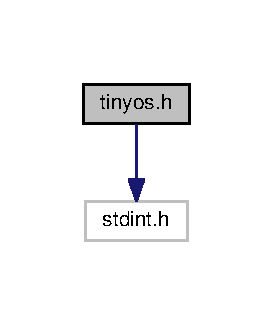
\includegraphics[width=131pt]{tinyos_8h__incl}
\end{center}
\end{figure}
This graph shows which files directly or indirectly include this file\+:\nopagebreak
\begin{figure}[H]
\begin{center}
\leavevmode
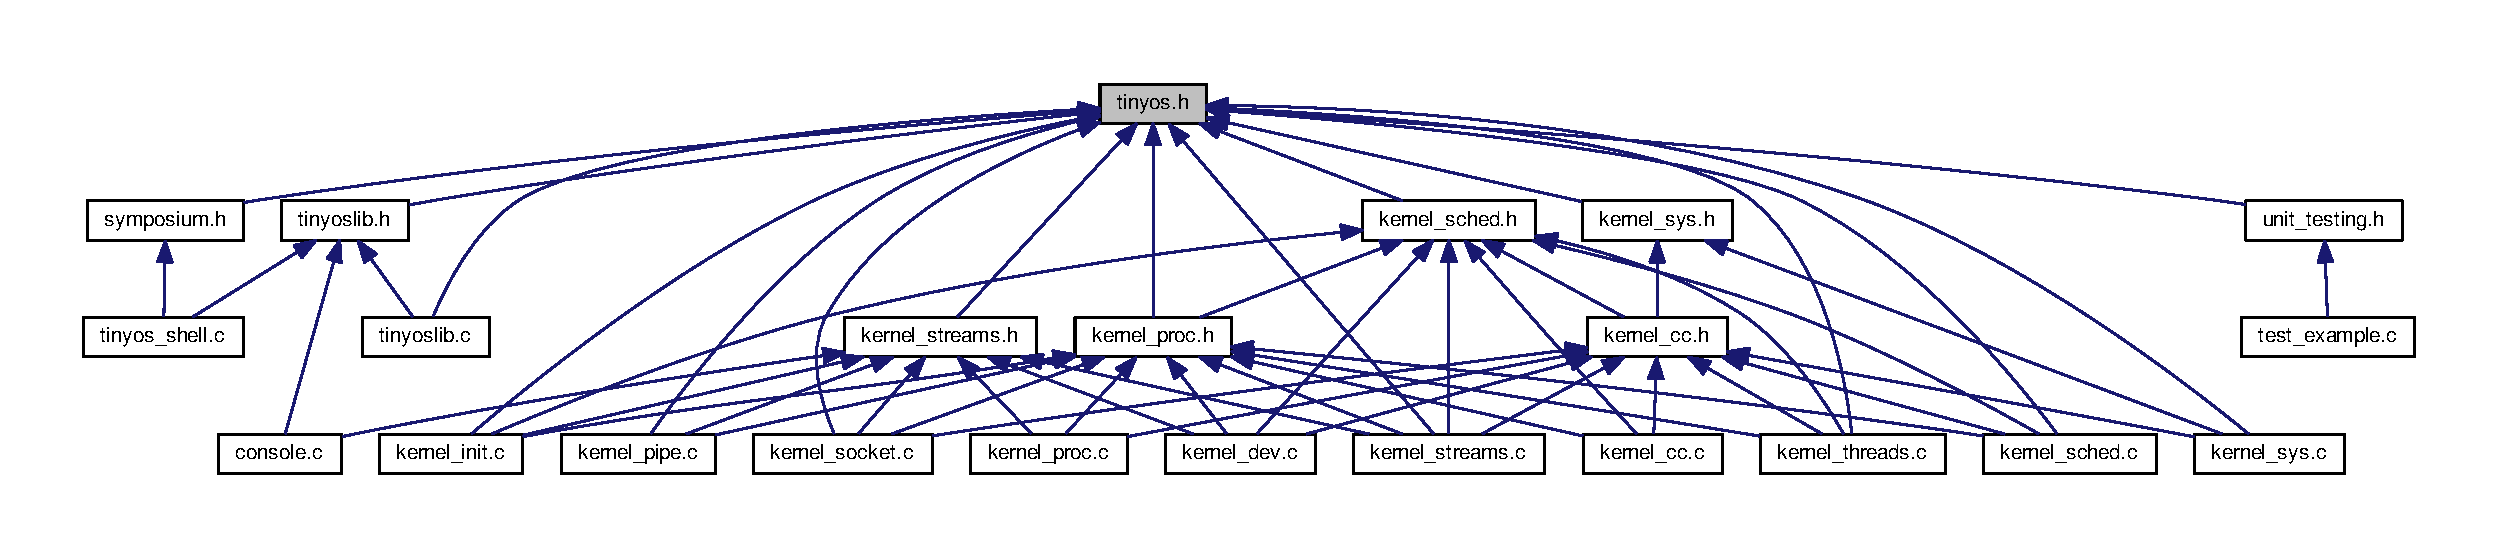
\includegraphics[width=350pt]{tinyos_8h__dep__incl}
\end{center}
\end{figure}
\subsection*{Data Structures}
\begin{DoxyCompactItemize}
\item 
struct \hyperlink{structCondVar}{Cond\+Var}
\begin{DoxyCompactList}\small\item\em Condition variables. \end{DoxyCompactList}\item 
struct \hyperlink{structpipe__s}{pipe\+\_\+s}
\begin{DoxyCompactList}\small\item\em A pair of file ids, describing a pipe. \end{DoxyCompactList}\item 
struct \hyperlink{structprocinfo}{procinfo}
\begin{DoxyCompactList}\small\item\em A struct containing process-\/related information for a non-\/free pid. \end{DoxyCompactList}\end{DoxyCompactItemize}
\subsection*{Macros}
\begin{DoxyCompactItemize}
\item 
\#define \hyperlink{group__syscalls_gaf22d54bd4d558803b5ccbc6eb21f83b2}{N\+O\+P\+R\+OC}~(-\/1)
\begin{DoxyCompactList}\small\item\em The invalid P\+ID. \end{DoxyCompactList}\item 
\#define \hyperlink{group__syscalls_ga63e32d00bc48471b4db49d481ac228dc}{M\+A\+X\+\_\+\+P\+R\+OC}~65536
\begin{DoxyCompactList}\small\item\em The maximum number of processes. \end{DoxyCompactList}\item 
\#define \hyperlink{group__syscalls_ga9c697bf9e856897ad75f28190a6f0b68}{M\+A\+X\+\_\+\+F\+I\+L\+E\+ID}~16
\begin{DoxyCompactList}\small\item\em The maximum number of open files per process. Only values 0 to M\+A\+X\+\_\+\+F\+I\+L\+E\+I\+D-\/1 are legal for file descriptors. \end{DoxyCompactList}\item 
\#define \hyperlink{group__syscalls_ga80bacbaea8dd6aecf216d85d981bcb21}{N\+O\+F\+I\+LE}~(-\/1)
\begin{DoxyCompactList}\small\item\em The invalid file id. \end{DoxyCompactList}\item 
\#define \hyperlink{group__syscalls_ga00ccfb785dd0b09ec7091fc213c2f491}{N\+O\+T\+H\+R\+E\+AD}~((\hyperlink{group__syscalls_gaf67ad1c55e6b2a79bf8a99106380ce01}{Tid\+\_\+t})0)
\begin{DoxyCompactList}\small\item\em The invalid thread ID. \end{DoxyCompactList}\item 
\#define \hyperlink{group__syscalls_ga96be0bfc33e7e113099c7546798bec99}{M\+U\+T\+E\+X\+\_\+\+I\+N\+IT}~0
\begin{DoxyCompactList}\small\item\em This macro is used to initialize mutexes. \end{DoxyCompactList}\item 
\#define \hyperlink{group__syscalls_ga6a7055a466bff255172e05f6ec82d792}{C\+O\+N\+D\+\_\+\+I\+N\+IT}~((\hyperlink{structCondVar}{Cond\+Var})\{ N\+U\+LL, \hyperlink{group__syscalls_ga96be0bfc33e7e113099c7546798bec99}{M\+U\+T\+E\+X\+\_\+\+I\+N\+IT} \})
\begin{DoxyCompactList}\small\item\em This macro is used to initialize condition variables. \end{DoxyCompactList}\item 
\#define \hyperlink{group__syscalls_ga401e1a60d6381236216b6a130a6685bd}{M\+A\+X\+\_\+\+P\+O\+RT}~1023
\begin{DoxyCompactList}\small\item\em the maximum legal port \end{DoxyCompactList}\item 
\#define \hyperlink{group__syscalls_gab71912b8841547d43a65ad40d730acd5}{N\+O\+P\+O\+RT}~((\hyperlink{group__syscalls_ga13894e5a2ffd5febb7aeb90e87239d61}{port\+\_\+t})0)
\begin{DoxyCompactList}\small\item\em a null value for a port \end{DoxyCompactList}\item 
\#define \hyperlink{group__syscalls_ga657ad9e9d81dcca25fb225cf99051e0d}{P\+R\+O\+C\+I\+N\+F\+O\+\_\+\+M\+A\+X\+\_\+\+A\+R\+G\+S\+\_\+\+S\+I\+ZE}~(128)
\begin{DoxyCompactList}\small\item\em The max. size of args returned by a procinfo structure. \end{DoxyCompactList}\end{DoxyCompactItemize}
\subsection*{Typedefs}
\begin{DoxyCompactItemize}
\item 
typedef int \hyperlink{group__syscalls_gafac07f3170763932fac97b6eab2c3984}{Pid\+\_\+t}
\begin{DoxyCompactList}\small\item\em The type of a process ID. \end{DoxyCompactList}\item 
typedef unsigned long \hyperlink{group__syscalls_gaf412159e5cef839836a5e7b19ee75d1c}{timeout\+\_\+t}
\begin{DoxyCompactList}\small\item\em An integer type for time intervals. \end{DoxyCompactList}\item 
typedef int \hyperlink{group__syscalls_ga5097222c5f0da97d92d4712359abc38f}{Fid\+\_\+t}
\begin{DoxyCompactList}\small\item\em The type of a file ID. \end{DoxyCompactList}\item 
typedef uintptr\+\_\+t \hyperlink{group__syscalls_gaf67ad1c55e6b2a79bf8a99106380ce01}{Tid\+\_\+t}
\begin{DoxyCompactList}\small\item\em The type of a thread ID. \end{DoxyCompactList}\item 
typedef char \hyperlink{group__syscalls_gaef2ec62cae8e0031fd19fc8b91083ade}{Mutex}
\begin{DoxyCompactList}\small\item\em A mutex is used to provide mutual exclusion. \end{DoxyCompactList}\item 
typedef int($\ast$ \hyperlink{group__syscalls_gaec3f2f835e105271fbbc00272c0ba984}{Task}) (int, void $\ast$)
\begin{DoxyCompactList}\small\item\em The signature for the main function of a process. \end{DoxyCompactList}\item 
typedef struct \hyperlink{structpipe__s}{pipe\+\_\+s} \hyperlink{group__syscalls_gad56b5ceaaf7d3ab88b4be7f622314dfb}{pipe\+\_\+t}
\begin{DoxyCompactList}\small\item\em A pair of file ids, describing a pipe. \end{DoxyCompactList}\item 
typedef int16\+\_\+t \hyperlink{group__syscalls_ga13894e5a2ffd5febb7aeb90e87239d61}{port\+\_\+t}
\begin{DoxyCompactList}\small\item\em A type for socket ports. \end{DoxyCompactList}\item 
typedef struct \hyperlink{structprocinfo}{procinfo} \hyperlink{group__syscalls_ga9682d9066f643f8d18cff58fd3fb09b9}{procinfo}
\begin{DoxyCompactList}\small\item\em A struct containing process-\/related information for a non-\/free pid. \end{DoxyCompactList}\end{DoxyCompactItemize}
\subsection*{Enumerations}
\begin{DoxyCompactItemize}
\item 
enum \hyperlink{group__syscalls_ga9eb10a0a72ca3149140272e9344a272b}{shutdown\+\_\+mode} \{ \hyperlink{group__syscalls_gga9eb10a0a72ca3149140272e9344a272bacbd27e0b4e3d4a02b0d833f919887d2d}{S\+H\+U\+T\+D\+O\+W\+N\+\_\+\+R\+E\+AD} =1, 
\hyperlink{group__syscalls_gga9eb10a0a72ca3149140272e9344a272ba9a7920b6a1eb57633bb981aa60edbe24}{S\+H\+U\+T\+D\+O\+W\+N\+\_\+\+W\+R\+I\+TE} =2, 
\hyperlink{group__syscalls_gga9eb10a0a72ca3149140272e9344a272bab67e72e17566af8eb432d0f3eba6d44d}{S\+H\+U\+T\+D\+O\+W\+N\+\_\+\+B\+O\+TH} =3
 \}\begin{DoxyCompactList}\small\item\em Socket shutdown modes. \end{DoxyCompactList}
\end{DoxyCompactItemize}
\subsection*{Functions}
\begin{DoxyCompactItemize}
\item 
void \hyperlink{group__syscalls_ga1140be44df71d39edaf6a7262fb763ca}{Mutex\+\_\+\+Lock} (\hyperlink{group__syscalls_gaef2ec62cae8e0031fd19fc8b91083ade}{Mutex} $\ast$)
\begin{DoxyCompactList}\small\item\em Lock a mutex. \end{DoxyCompactList}\item 
void \hyperlink{group__syscalls_ga0b98d0315d0931d0c28104c36dd559c9}{Mutex\+\_\+\+Unlock} (\hyperlink{group__syscalls_gaef2ec62cae8e0031fd19fc8b91083ade}{Mutex} $\ast$)
\begin{DoxyCompactList}\small\item\em Unlock a mutex that you locked. \end{DoxyCompactList}\item 
int \hyperlink{group__syscalls_ga970dca2210b3f2ec8aedab7f542a9bf4}{Cond\+\_\+\+Wait} (\hyperlink{group__syscalls_gaef2ec62cae8e0031fd19fc8b91083ade}{Mutex} $\ast$mx, \hyperlink{structCondVar}{Cond\+Var} $\ast$cv)
\begin{DoxyCompactList}\small\item\em Wait on a condition variable. \end{DoxyCompactList}\item 
int \hyperlink{group__syscalls_ga4e955b769339be9ea6a0c1bd4151c48f}{Cond\+\_\+\+Timed\+Wait} (\hyperlink{group__syscalls_gaef2ec62cae8e0031fd19fc8b91083ade}{Mutex} $\ast$mx, \hyperlink{structCondVar}{Cond\+Var} $\ast$cv, \hyperlink{group__syscalls_gaf412159e5cef839836a5e7b19ee75d1c}{timeout\+\_\+t} timeout)
\begin{DoxyCompactList}\small\item\em Wait on a condition variable. \end{DoxyCompactList}\item 
void \hyperlink{group__syscalls_ga43f64f8be273d2fe77d7de5f4b81e22d}{Cond\+\_\+\+Signal} (\hyperlink{structCondVar}{Cond\+Var} $\ast$)
\begin{DoxyCompactList}\small\item\em Signal a condition variable. \end{DoxyCompactList}\item 
void \hyperlink{group__syscalls_ga8196aa2a48cad90742f254cc3b8fd351}{Cond\+\_\+\+Broadcast} (\hyperlink{structCondVar}{Cond\+Var} $\ast$)
\begin{DoxyCompactList}\small\item\em Notify all threads waiting at a condition variable. \end{DoxyCompactList}\item 
\hyperlink{group__syscalls_gafac07f3170763932fac97b6eab2c3984}{Pid\+\_\+t} \hyperlink{group__syscalls_ga737ad30d8105b4b76e3eb102dd016404}{Exec} (\hyperlink{group__syscalls_gaec3f2f835e105271fbbc00272c0ba984}{Task} task, int argl, void $\ast$args)
\begin{DoxyCompactList}\small\item\em Create a new process. \end{DoxyCompactList}\item 
void \hyperlink{group__syscalls_gabed0249344c12ecd4f8d440fc05a360a}{Exit} (int val)
\begin{DoxyCompactList}\small\item\em Exit the current process. \end{DoxyCompactList}\item 
\hyperlink{group__syscalls_gafac07f3170763932fac97b6eab2c3984}{Pid\+\_\+t} \hyperlink{group__syscalls_ga37017afba05480740d26b033975fef03}{Wait\+Child} (\hyperlink{group__syscalls_gafac07f3170763932fac97b6eab2c3984}{Pid\+\_\+t} pid, int $\ast$exitval)
\begin{DoxyCompactList}\small\item\em Wait on a terminating child. \end{DoxyCompactList}\item 
\hyperlink{group__syscalls_gafac07f3170763932fac97b6eab2c3984}{Pid\+\_\+t} \hyperlink{group__syscalls_ga5106ac1f078c5dde2d6fea3881c1a4fb}{Get\+Pid} (void)
\begin{DoxyCompactList}\small\item\em Return the P\+ID of the caller. \end{DoxyCompactList}\item 
\hyperlink{group__syscalls_gafac07f3170763932fac97b6eab2c3984}{Pid\+\_\+t} \hyperlink{group__syscalls_ga33ccb3f7c80d85e610206c0e1150657b}{Get\+P\+Pid} (void)
\begin{DoxyCompactList}\small\item\em Return the P\+ID of the caller\textquotesingle{}s parent. \end{DoxyCompactList}\item 
\hyperlink{group__syscalls_gaf67ad1c55e6b2a79bf8a99106380ce01}{Tid\+\_\+t} \hyperlink{group__syscalls_ga284070b5fddcc3653e146e63fcbfe6e3}{Create\+Thread} (\hyperlink{group__syscalls_gaec3f2f835e105271fbbc00272c0ba984}{Task} task, int argl, void $\ast$args)
\begin{DoxyCompactList}\small\item\em Create a new thread in the current process. \end{DoxyCompactList}\item 
\hyperlink{group__syscalls_gaf67ad1c55e6b2a79bf8a99106380ce01}{Tid\+\_\+t} \hyperlink{group__syscalls_ga75ffeb50fda6297110a2f07ef94d285c}{Thread\+Self} ()
\begin{DoxyCompactList}\small\item\em Return the Tid of the current thread. \end{DoxyCompactList}\item 
int \hyperlink{group__syscalls_ga9ffbb344eb33487ceef5442846a74be0}{Thread\+Join} (\hyperlink{group__syscalls_gaf67ad1c55e6b2a79bf8a99106380ce01}{Tid\+\_\+t} tid, int $\ast$exitval)
\begin{DoxyCompactList}\small\item\em Join the given thread. \end{DoxyCompactList}\item 
int \hyperlink{group__syscalls_ga5f957d985678728a418ff70a617fab4d}{Thread\+Detach} (\hyperlink{group__syscalls_gaf67ad1c55e6b2a79bf8a99106380ce01}{Tid\+\_\+t} tid)
\begin{DoxyCompactList}\small\item\em Detach the given thread. \end{DoxyCompactList}\item 
void \hyperlink{group__syscalls_gab77e59bf31165db88a22ac8f031b8741}{Thread\+Exit} (int exitval)
\begin{DoxyCompactList}\small\item\em Terminate the current thread. \end{DoxyCompactList}\item 
unsigned int \hyperlink{group__syscalls_ga31576e1579c15b6b066038702e6557c7}{Get\+Terminal\+Devices} ()
\begin{DoxyCompactList}\small\item\em Return the number of terminal devices available. \end{DoxyCompactList}\item 
\hyperlink{group__syscalls_ga5097222c5f0da97d92d4712359abc38f}{Fid\+\_\+t} \hyperlink{group__syscalls_ga6ea2b586a8dfcfc1e7065e1664a0fb35}{Open\+Terminal} (unsigned int termno)
\begin{DoxyCompactList}\small\item\em Open a stream on terminal device \textquotesingle{}termno\textquotesingle{}. \end{DoxyCompactList}\item 
\hyperlink{group__syscalls_ga5097222c5f0da97d92d4712359abc38f}{Fid\+\_\+t} \hyperlink{group__syscalls_ga39805b4ae668b715fb43f0f1e6ce8c45}{Open\+Null} ()
\begin{DoxyCompactList}\small\item\em Open a stream on the null device. \end{DoxyCompactList}\item 
int \hyperlink{group__syscalls_ga3e9dc545a789eb45b2d356eabbac3ee3}{Read} (\hyperlink{group__syscalls_ga5097222c5f0da97d92d4712359abc38f}{Fid\+\_\+t} fd, char $\ast$buf, unsigned int size)
\begin{DoxyCompactList}\small\item\em Read bytes from a stream. \end{DoxyCompactList}\item 
int \hyperlink{group__syscalls_gaf046f003fde24f79fb395c250137856c}{Write} (\hyperlink{group__syscalls_ga5097222c5f0da97d92d4712359abc38f}{Fid\+\_\+t} fd, const char $\ast$buf, unsigned int size)
\begin{DoxyCompactList}\small\item\em Write bytes to a stream. \end{DoxyCompactList}\item 
int \hyperlink{group__syscalls_ga82187e2e98af053a2ab6cb516e9e7f5a}{Close} (\hyperlink{group__syscalls_ga5097222c5f0da97d92d4712359abc38f}{Fid\+\_\+t} fd)
\begin{DoxyCompactList}\small\item\em Close a file id. \end{DoxyCompactList}\item 
int \hyperlink{group__syscalls_gacc048c60209e2dfb4b5cfc1c3f21aa88}{Dup2} (\hyperlink{group__syscalls_ga5097222c5f0da97d92d4712359abc38f}{Fid\+\_\+t} oldfd, \hyperlink{group__syscalls_ga5097222c5f0da97d92d4712359abc38f}{Fid\+\_\+t} newfd)
\begin{DoxyCompactList}\small\item\em Make a copy of a stream to a new file ID. \end{DoxyCompactList}\item 
int \hyperlink{group__syscalls_gab6355ce54e047c31538ed5ed9108b5b3}{Pipe} (\hyperlink{group__syscalls_gad56b5ceaaf7d3ab88b4be7f622314dfb}{pipe\+\_\+t} $\ast$pipe)
\begin{DoxyCompactList}\small\item\em Construct and return a pipe. \end{DoxyCompactList}\item 
\hyperlink{group__syscalls_ga5097222c5f0da97d92d4712359abc38f}{Fid\+\_\+t} \hyperlink{group__syscalls_gadf167321edde68e905173d8056d3eb2f}{Socket} (\hyperlink{group__syscalls_ga13894e5a2ffd5febb7aeb90e87239d61}{port\+\_\+t} port)
\begin{DoxyCompactList}\small\item\em Return a new socket bound on a port. \end{DoxyCompactList}\item 
int \hyperlink{group__syscalls_ga9ff5bae3e7b9e5bbf5a788a5ff739bf7}{Listen} (\hyperlink{group__syscalls_ga5097222c5f0da97d92d4712359abc38f}{Fid\+\_\+t} sock)
\begin{DoxyCompactList}\small\item\em Initialize a socket as a listening socket. \end{DoxyCompactList}\item 
\hyperlink{group__syscalls_ga5097222c5f0da97d92d4712359abc38f}{Fid\+\_\+t} \hyperlink{group__syscalls_ga8116ee944d1b03b6fb2fdba59b57d4a8}{Accept} (\hyperlink{group__syscalls_ga5097222c5f0da97d92d4712359abc38f}{Fid\+\_\+t} lsock)
\begin{DoxyCompactList}\small\item\em Wait for a connection. \end{DoxyCompactList}\item 
int \hyperlink{group__syscalls_ga747ceadd43e9a4c72b08fffbadaefbdd}{Connect} (\hyperlink{group__syscalls_ga5097222c5f0da97d92d4712359abc38f}{Fid\+\_\+t} sock, \hyperlink{group__syscalls_ga13894e5a2ffd5febb7aeb90e87239d61}{port\+\_\+t} port, \hyperlink{group__syscalls_gaf412159e5cef839836a5e7b19ee75d1c}{timeout\+\_\+t} timeout)
\begin{DoxyCompactList}\small\item\em Create a connection to a listener at a specific port. \end{DoxyCompactList}\item 
int \hyperlink{group__syscalls_ga61d49d63d8c0f9fc0917cc1bda6fdfcb}{Shut\+Down} (\hyperlink{group__syscalls_ga5097222c5f0da97d92d4712359abc38f}{Fid\+\_\+t} sock, \hyperlink{group__syscalls_ga9eb10a0a72ca3149140272e9344a272b}{shutdown\+\_\+mode} how)
\begin{DoxyCompactList}\small\item\em Shut down one direction of socket communication. \end{DoxyCompactList}\item 
\hyperlink{group__syscalls_ga5097222c5f0da97d92d4712359abc38f}{Fid\+\_\+t} \hyperlink{group__syscalls_gaf326b11574cdc84a9e21b9d860076821}{Open\+Info} ()
\begin{DoxyCompactList}\small\item\em Open a kernel information stream. \end{DoxyCompactList}\item 
void \hyperlink{group__syscalls_ga31d9ee7df9665928617a9f9c0cc6d361}{boot} (unsigned int ncores, unsigned int terminals, \hyperlink{group__syscalls_gaec3f2f835e105271fbbc00272c0ba984}{Task} boot\+\_\+task, int argl, void $\ast$args)
\begin{DoxyCompactList}\small\item\em Boot tinyos3. \end{DoxyCompactList}\end{DoxyCompactItemize}


\subsection{Detailed Description}
Public kernel A\+PI. 


\hypertarget{tinyoslib_8h}{}\section{tinyoslib.\+h File Reference}
\label{tinyoslib_8h}\index{tinyoslib.\+h@{tinyoslib.\+h}}


Tiny\+OS standard library header file.  


{\ttfamily \#include $<$stdio.\+h$>$}\\*
{\ttfamily \#include \char`\"{}tinyos.\+h\char`\"{}}\\*
Include dependency graph for tinyoslib.\+h\+:\nopagebreak
\begin{figure}[H]
\begin{center}
\leavevmode
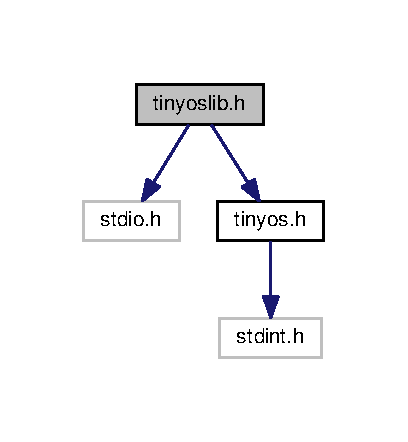
\includegraphics[width=196pt]{tinyoslib_8h__incl}
\end{center}
\end{figure}
This graph shows which files directly or indirectly include this file\+:\nopagebreak
\begin{figure}[H]
\begin{center}
\leavevmode
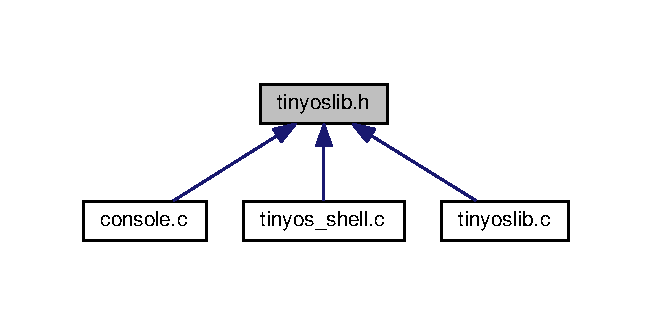
\includegraphics[width=313pt]{tinyoslib_8h__dep__incl}
\end{center}
\end{figure}
\subsection*{Typedefs}
\begin{DoxyCompactItemize}
\item 
typedef int($\ast$ \hyperlink{tinyoslib_8h_ab518accf2c30e915a8250c0ae308aefd}{Program}) (size\+\_\+t argc, const char $\ast$$\ast$argv)\hypertarget{tinyoslib_8h_ab518accf2c30e915a8250c0ae308aefd}{}\label{tinyoslib_8h_ab518accf2c30e915a8250c0ae308aefd}

\begin{DoxyCompactList}\small\item\em A declaration for C-\/like main programs. \end{DoxyCompactList}\end{DoxyCompactItemize}
\subsection*{Functions}
\begin{DoxyCompactItemize}
\item 
F\+I\+LE $\ast$ \hyperlink{tinyoslib_8h_a8f1a14eaa13a383f7c12be56abc4ff4d}{fidopen} (\hyperlink{group__syscalls_ga5097222c5f0da97d92d4712359abc38f}{Fid\+\_\+t} fid, const char $\ast$mode)
\begin{DoxyCompactList}\small\item\em Open a C stream on a tinyos file descriptor. \end{DoxyCompactList}\item 
void {\bfseries tinyos\+\_\+replace\+\_\+stdio} ()\hypertarget{tinyoslib_8h_a4b99e52f6d50e0f1d1080cf59beab04b}{}\label{tinyoslib_8h_a4b99e52f6d50e0f1d1080cf59beab04b}

\item 
void {\bfseries tinyos\+\_\+restore\+\_\+stdio} ()\hypertarget{tinyoslib_8h_a6e78397853f151751db73e9b400ca4ce}{}\label{tinyoslib_8h_a6e78397853f151751db73e9b400ca4ce}

\item 
void {\bfseries tinyos\+\_\+pseudo\+\_\+console} ()\hypertarget{tinyoslib_8h_a5fccd2ce8700c35cdef057a45e0f72ed}{}\label{tinyoslib_8h_a5fccd2ce8700c35cdef057a45e0f72ed}

\item 
int \hyperlink{tinyoslib_8h_a0e11b5da87f467679adbb23883328c2d}{Execute} (\hyperlink{tinyoslib_8h_ab518accf2c30e915a8250c0ae308aefd}{Program} prog, size\+\_\+t argc, const char $\ast$$\ast$argv)
\begin{DoxyCompactList}\small\item\em Execute a new process, passing it the given arguments. \end{DoxyCompactList}\item 
int \hyperlink{tinyoslib_8h_ab98738d69f4b198fbcad1a6f2e20a44d}{Parse\+Proc\+Info} (\hyperlink{structprocinfo}{procinfo} $\ast$pinfo, \hyperlink{tinyoslib_8h_ab518accf2c30e915a8250c0ae308aefd}{Program} $\ast$prog, int argc, const char $\ast$$\ast$argv)
\begin{DoxyCompactList}\small\item\em Try to reclaim the arguments of a process. \end{DoxyCompactList}\end{DoxyCompactItemize}


\subsection{Detailed Description}
Tiny\+OS standard library header file. 

Small non-\/kernel routines for wrapping tinyos functionality go here. 

\subsection{Function Documentation}
\index{tinyoslib.\+h@{tinyoslib.\+h}!Execute@{Execute}}
\index{Execute@{Execute}!tinyoslib.\+h@{tinyoslib.\+h}}
\subsubsection[{\texorpdfstring{Execute(\+Program prog, size\+\_\+t argc, const char $\ast$$\ast$argv)}{Execute(Program prog, size_t argc, const char **argv)}}]{\setlength{\rightskip}{0pt plus 5cm}int Execute (
\begin{DoxyParamCaption}
\item[{{\bf Program}}]{prog, }
\item[{size\+\_\+t}]{argc, }
\item[{const char $\ast$$\ast$}]{argv}
\end{DoxyParamCaption}
)}\hypertarget{tinyoslib_8h_a0e11b5da87f467679adbb23883328c2d}{}\label{tinyoslib_8h_a0e11b5da87f467679adbb23883328c2d}


Execute a new process, passing it the given arguments. 

The underlying implementation uses the Exec system call, to create a new process.

By convention, argument argv\mbox{[}0\mbox{]} is assumed to be the program name, although any string is actually acceptable. 

Definition at line 147 of file tinyoslib.\+c.

\index{tinyoslib.\+h@{tinyoslib.\+h}!fidopen@{fidopen}}
\index{fidopen@{fidopen}!tinyoslib.\+h@{tinyoslib.\+h}}
\subsubsection[{\texorpdfstring{fidopen(\+Fid\+\_\+t fid, const char $\ast$mode)}{fidopen(Fid_t fid, const char *mode)}}]{\setlength{\rightskip}{0pt plus 5cm}F\+I\+LE$\ast$ fidopen (
\begin{DoxyParamCaption}
\item[{{\bf Fid\+\_\+t}}]{fid, }
\item[{const char $\ast$}]{mode}
\end{DoxyParamCaption}
)}\hypertarget{tinyoslib_8h_a8f1a14eaa13a383f7c12be56abc4ff4d}{}\label{tinyoslib_8h_a8f1a14eaa13a383f7c12be56abc4ff4d}


Open a C stream on a tinyos file descriptor. 

This call returns a new F\+I\+LE pointer on success and N\+U\+LL on failure. 

Definition at line 49 of file tinyoslib.\+c.

\index{tinyoslib.\+h@{tinyoslib.\+h}!Parse\+Proc\+Info@{Parse\+Proc\+Info}}
\index{Parse\+Proc\+Info@{Parse\+Proc\+Info}!tinyoslib.\+h@{tinyoslib.\+h}}
\subsubsection[{\texorpdfstring{Parse\+Proc\+Info(procinfo $\ast$pinfo, Program $\ast$prog, int argc, const char $\ast$$\ast$argv)}{ParseProcInfo(procinfo *pinfo, Program *prog, int argc, const char **argv)}}]{\setlength{\rightskip}{0pt plus 5cm}int Parse\+Proc\+Info (
\begin{DoxyParamCaption}
\item[{{\bf procinfo} $\ast$}]{pinfo, }
\item[{{\bf Program} $\ast$}]{prog, }
\item[{int}]{argc, }
\item[{const char $\ast$$\ast$}]{argv}
\end{DoxyParamCaption}
)}\hypertarget{tinyoslib_8h_ab98738d69f4b198fbcad1a6f2e20a44d}{}\label{tinyoslib_8h_ab98738d69f4b198fbcad1a6f2e20a44d}


Try to reclaim the arguments of a process. 

Given a \hyperlink{structprocinfo}{procinfo} object returned by a \hyperlink{group__syscalls_gaf326b11574cdc84a9e21b9d860076821}{Open\+Info} stream, if this process was executed by \hyperlink{tinyoslib_8h_a0e11b5da87f467679adbb23883328c2d}{Execute}, try to reclaim the arguments passed to it.

If the process was not executed by \hyperlink{tinyoslib_8h_a0e11b5da87f467679adbb23883328c2d}{Execute}, or if its arguments were too long, this effort may fail, in which case -\/1 is returned.

Else, the {\ttfamily pinfo} argument buffer defined by {\ttfamily (pinfo-\/$>$argl, pinfo-\/$>$args)} is parsed. Let it contain {\ttfamily N} arguments. Then,
\begin{DoxyItemize}
\item if {\ttfamily prog} is non-\/\+N\+U\+LL, {\ttfamily $\ast$prog} is filled with a pointer to the function executed by {\ttfamily Execute} 
\item if {\ttfamily argv} is non-\/\+N\+U\+LL, it is assumed that it points to an array of strings, of size argc. Then, min(argc, N) locations of this array are initialized from the arguments of {\ttfamily pinfo}.
\item finally, N is returned.
\end{DoxyItemize}


\begin{DoxyParams}{Parameters}
{\em pinfo} & the procinfo object to process. \\
\hline
{\em prog} & if not N\+U\+LL, the location to hold the program\textquotesingle{}s address. \\
\hline
{\em argc} & the length of parameter {\ttfamily argv} \\
\hline
{\em argv} & if not N\+U\+LL, a string vector of size argc \\
\hline
\end{DoxyParams}
\begin{DoxyReturn}{Returns}
if {\ttfamily pinfo} is successfully parsed, the number of arguments is returned, else -\/1 is returned. 
\end{DoxyReturn}


Definition at line 115 of file tinyoslib.\+c.


\hypertarget{unit__testing_8h}{}\section{unit\+\_\+testing.\+h File Reference}
\label{unit__testing_8h}\index{unit\+\_\+testing.\+h@{unit\+\_\+testing.\+h}}


A library for coding and running unit tests.  


{\ttfamily \#include \char`\"{}bios.\+h\char`\"{}}\\*
{\ttfamily \#include \char`\"{}tinyos.\+h\char`\"{}}\\*
Include dependency graph for unit\+\_\+testing.\+h\+:\nopagebreak
\begin{figure}[H]
\begin{center}
\leavevmode
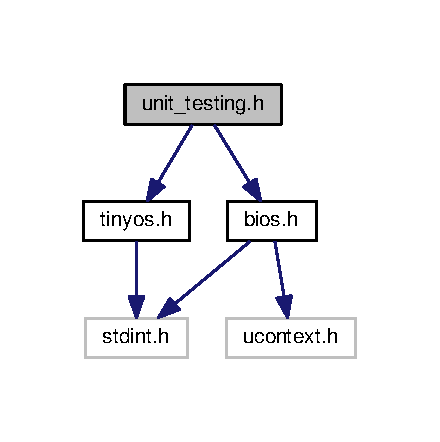
\includegraphics[width=211pt]{unit__testing_8h__incl}
\end{center}
\end{figure}
This graph shows which files directly or indirectly include this file\+:\nopagebreak
\begin{figure}[H]
\begin{center}
\leavevmode
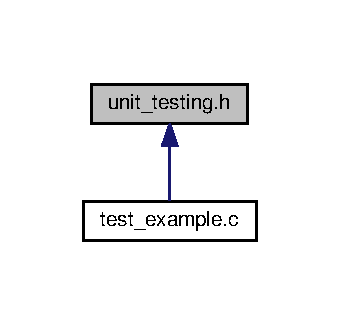
\includegraphics[width=163pt]{unit__testing_8h__dep__incl}
\end{center}
\end{figure}
\subsection*{Data Structures}
\begin{DoxyCompactItemize}
\item 
struct \hyperlink{structprogram__arguments}{program\+\_\+arguments}
\begin{DoxyCompactList}\small\item\em Global arguments for test execution. \end{DoxyCompactList}\item 
struct \hyperlink{structTest}{Test}
\begin{DoxyCompactList}\small\item\em \hyperlink{structTest}{Test} descriptor. \end{DoxyCompactList}\end{DoxyCompactItemize}
\subsection*{Macros}
\begin{DoxyCompactItemize}
\item 
\#define \hyperlink{group__Testing_ga2a77d2f2c5b698c69c19e1f8782bf709}{M\+A\+X\+\_\+\+T\+E\+S\+TS}~1024
\begin{DoxyCompactList}\small\item\em Maximum number of tests on the command line. \end{DoxyCompactList}\item 
\#define \hyperlink{group__Testing_ga9be407f8744aff436633d34c62591cb9}{A\+S\+S\+E\+R\+T\+\_\+\+M\+SG}(expr,  format, ...)
\begin{DoxyCompactList}\small\item\em Like A\+S\+S\+E\+RT but with a custom message. \end{DoxyCompactList}\item 
\#define \hyperlink{group__Testing_ga28301f76c53b643912da7c538f74e2c6}{A\+S\+S\+E\+RT}(expr)~\hyperlink{group__Testing_ga9be407f8744aff436633d34c62591cb9}{A\+S\+S\+E\+R\+T\+\_\+\+M\+SG}(expr, \char`\"{}\%s(\%d)\+: A\+S\+S\+E\+RT failed\+: \%s \textbackslash{}n\char`\"{},\+\_\+\+\_\+\+F\+I\+L\+E\+\_\+\+\_\+, \+\_\+\+\_\+\+L\+I\+N\+E\+\_\+\+\_\+, \#expr)
\begin{DoxyCompactList}\small\item\em Fail the test if an expression is false. \end{DoxyCompactList}\item 
\#define \hyperlink{group__Testing_ga1ac76218e138d4f495b9a695c5da5b9b}{F\+U\+D\+GE}(var)~memset(\&(var), 170, sizeof(var))
\begin{DoxyCompactList}\small\item\em Fill in the bytes of a variable with a weird value\+: 10101010 or 0x\+AA. \end{DoxyCompactList}\item 
\#define \hyperlink{group__Testing_gaad2dd72565852b91c809cd4685833b17}{D\+E\+F\+A\+U\+L\+T\+\_\+\+T\+I\+M\+E\+O\+UT}~10
\begin{DoxyCompactList}\small\item\em Default time per test. \end{DoxyCompactList}\item 
\#define \hyperlink{group__Testing_gadeb59351f026036674baa906f32ccd5c}{B\+A\+R\+E\+\_\+\+T\+E\+ST}(tname,  descr, ...)
\begin{DoxyCompactList}\small\item\em Declare a standard test function. \end{DoxyCompactList}\item 
\#define \hyperlink{group__Testing_gadaaab439c094503b6ed7c313ad082f10}{B\+O\+O\+T\+\_\+\+T\+E\+ST}(tname,  descr, ...)
\begin{DoxyCompactList}\small\item\em Declare a test function run as the boot function of the tinyos kernel. \end{DoxyCompactList}\item 
\#define \hyperlink{group__Testing_ga3e52396e466caa8cba74e1ae603817d3}{T\+E\+S\+T\+\_\+\+S\+U\+I\+TE}(tname,  descr, ...)
\begin{DoxyCompactList}\small\item\em Declare a collectio of test functions. \end{DoxyCompactList}\end{DoxyCompactItemize}
\subsection*{Typedefs}
\begin{DoxyCompactItemize}
\item 
typedef struct \hyperlink{structTest}{Test} \hyperlink{group__Testing_ga8900225cc98bb7c7fb170b8694e1f7a4}{Test}
\begin{DoxyCompactList}\small\item\em \hyperlink{structTest}{Test} descriptor. \end{DoxyCompactList}\end{DoxyCompactItemize}
\subsection*{Enumerations}
\begin{DoxyCompactItemize}
\item 
enum {\bfseries Test\+\_\+type} \{ {\bfseries N\+O\+\_\+\+F\+U\+NC}, 
{\bfseries B\+A\+R\+E\+\_\+\+F\+U\+NC}, 
{\bfseries B\+O\+O\+T\+\_\+\+F\+U\+NC}, 
{\bfseries S\+U\+I\+T\+E\+\_\+\+F\+U\+NC}
 \}\hypertarget{group__Testing_gae6e489086f229b5c8289c94fba0244fa}{}\label{group__Testing_gae6e489086f229b5c8289c94fba0244fa}

\end{DoxyCompactItemize}
\subsection*{Functions}
\begin{DoxyCompactItemize}
\item 
void \hyperlink{group__Testing_ga2e36933a48fbca44bb782f881ddceb20}{M\+SG} (const char $\ast$format,...) \+\_\+\+\_\+attribute\+\_\+\+\_\+((format(printf
\begin{DoxyCompactList}\small\item\em Print formatted messages. \end{DoxyCompactList}\item 
void \hyperlink{group__Testing_ga0c4e801b8c3317b802fa4e80e1e26de2}{expect} (\hyperlink{bios_8h_a91ad9478d81a7aaf2593e8d9c3d06a14}{uint} term, const char $\ast$pattern)
\begin{DoxyCompactList}\small\item\em Expect to see some bytes printed to terminal. \end{DoxyCompactList}\item 
void \hyperlink{group__Testing_ga0f97d30c4cd1370bcac6d7f4775d6789}{sendme} (\hyperlink{bios_8h_a91ad9478d81a7aaf2593e8d9c3d06a14}{uint} term, const char $\ast$pattern)
\begin{DoxyCompactList}\small\item\em Ask to receive some bytes from the keyboard. \end{DoxyCompactList}\item 
int \hyperlink{group__Testing_gac023795199b4f577a9181ac45e62b170}{run\+\_\+test} (const \hyperlink{structTest}{Test} $\ast$test)
\begin{DoxyCompactList}\small\item\em The main routine to run a test. \end{DoxyCompactList}\item 
int \hyperlink{group__Testing_ga4663cf3fb390b2a6d9cf1943f21b9934}{register\+\_\+test} (const \hyperlink{structTest}{Test} $\ast$test)
\begin{DoxyCompactList}\small\item\em Called from the main program to register a test (usually a suite). \end{DoxyCompactList}\item 
int \hyperlink{group__Testing_ga91dbdb97056588b088b689582abc2382}{run\+\_\+program} (int argc, char $\ast$$\ast$argv, const \hyperlink{structTest}{Test} $\ast$default\+\_\+test)
\begin{DoxyCompactList}\small\item\em Called from the main program to parse arguments and run tests. \end{DoxyCompactList}\end{DoxyCompactItemize}
\subsection*{Variables}
\begin{DoxyCompactItemize}
\item 
struct \hyperlink{structprogram__arguments}{program\+\_\+arguments} \hyperlink{group__Testing_ga0bc61f89e22f48a0af7de4659a69c6f2}{A\+R\+GS}
\item 
void int \hyperlink{group__Testing_ga35895e417ef253455c9cf365cb66d87c}{F\+L\+A\+G\+\_\+\+F\+A\+I\+L\+U\+RE}
\begin{DoxyCompactList}\small\item\em Flag failure during a test. \end{DoxyCompactList}\end{DoxyCompactItemize}


\subsection{Detailed Description}
A library for coding and running unit tests. 


\hypertarget{util_8h}{}\section{util.\+h File Reference}
\label{util_8h}\index{util.\+h@{util.\+h}}


Tinyos utility code.  


{\ttfamily \#include $<$stdlib.\+h$>$}\\*
{\ttfamily \#include $<$stdio.\+h$>$}\\*
{\ttfamily \#include $<$stdint.\+h$>$}\\*
{\ttfamily \#include $<$string.\+h$>$}\\*
{\ttfamily \#include $<$errno.\+h$>$}\\*
{\ttfamily \#include $<$setjmp.\+h$>$}\\*
{\ttfamily \#include $<$assert.\+h$>$}\\*
Include dependency graph for util.\+h\+:\nopagebreak
\begin{figure}[H]
\begin{center}
\leavevmode
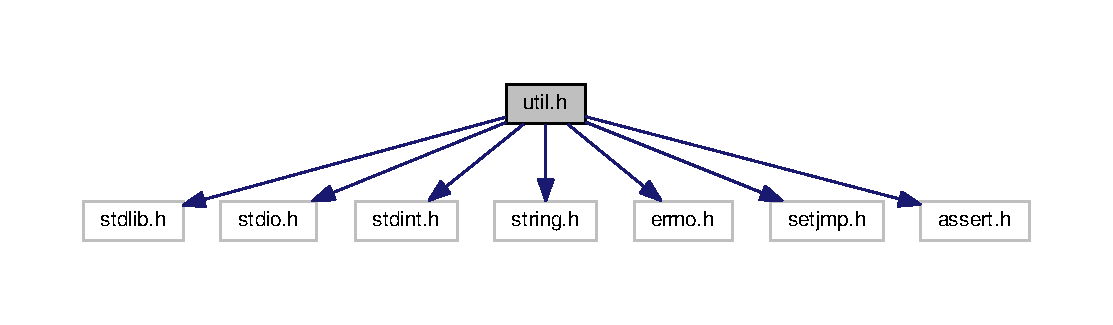
\includegraphics[width=350pt]{util_8h__incl}
\end{center}
\end{figure}
This graph shows which files directly or indirectly include this file\+:\nopagebreak
\begin{figure}[H]
\begin{center}
\leavevmode
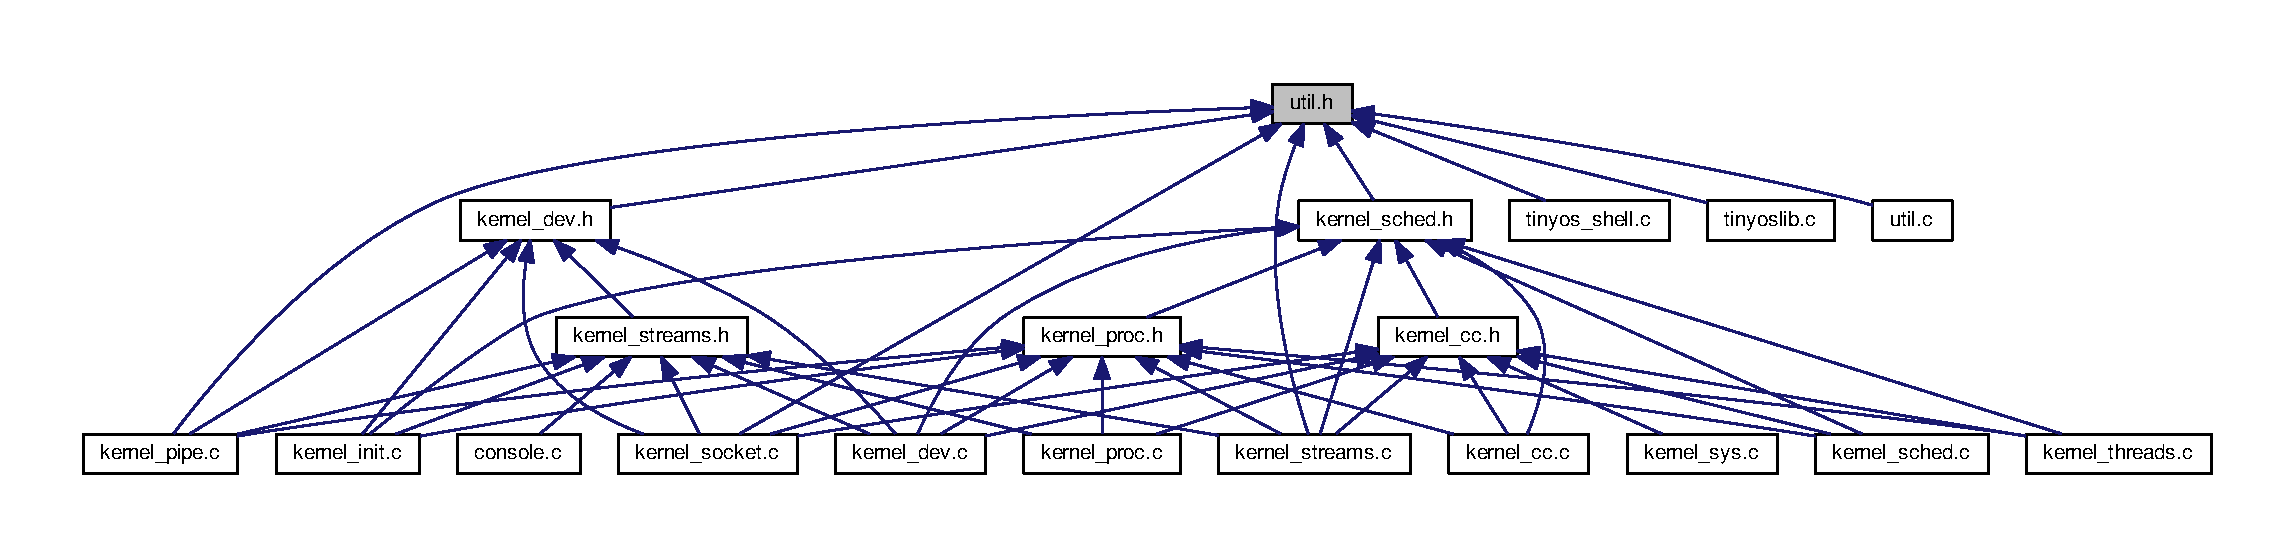
\includegraphics[width=350pt]{util_8h__dep__incl}
\end{center}
\end{figure}
\subsection*{Data Structures}
\begin{DoxyCompactItemize}
\item 
struct \hyperlink{structresource__list__node}{resource\+\_\+list\+\_\+node}
\begin{DoxyCompactList}\small\item\em List node. \end{DoxyCompactList}\item 
struct \hyperlink{structexception__handler__frame}{exception\+\_\+handler\+\_\+frame}
\item 
struct \hyperlink{structexception__stack__frame}{exception\+\_\+stack\+\_\+frame}
\end{DoxyCompactItemize}
\subsection*{Macros}
\begin{DoxyCompactItemize}
\item 
\#define \hyperlink{group__check__macros_ga7a3e1d362790a375466c5e77a6d5c9c5}{F\+A\+T\+AL}(msg)
\begin{DoxyCompactList}\small\item\em Print a message to stderr and abort. \end{DoxyCompactList}\item 
\#define \hyperlink{group__check__macros_gab2b3925a76d34a1272ace73af5a81945}{F\+A\+T\+A\+L\+E\+RR}(errcode)~\hyperlink{group__check__macros_ga7a3e1d362790a375466c5e77a6d5c9c5}{F\+A\+T\+AL}(strerror(errcode))
\begin{DoxyCompactList}\small\item\em Print an error message to stderr and abort. \end{DoxyCompactList}\item 
\#define \hyperlink{group__check__macros_ga879857ca00d32faa0d6cfe416428a804}{C\+H\+E\+C\+K\+RC}(cmd)~\{ int rc = (cmd); if(rc) \hyperlink{group__check__macros_gab2b3925a76d34a1272ace73af5a81945}{F\+A\+T\+A\+L\+E\+RR}(rc); \}
\begin{DoxyCompactList}\small\item\em Wrap a unix call to check for errors. \end{DoxyCompactList}\item 
\#define \hyperlink{group__check__macros_ga1992445028206dcca9c93c9a0b558436}{C\+H\+E\+CK}(cmd)~\{ if((cmd)==-\/1) \hyperlink{group__check__macros_gab2b3925a76d34a1272ace73af5a81945}{F\+A\+T\+A\+L\+E\+RR}(errno); \}
\begin{DoxyCompactList}\small\item\em Wrap a unix call to check for errors. \end{DoxyCompactList}\item 
\#define \hyperlink{group__check__macros_ga6196238e8ab53ab90e7bf7ab51fc73e9}{C\+H\+E\+C\+K\+\_\+\+C\+O\+N\+D\+I\+T\+I\+ON}(expr)~\{ if(!(expr)) \hyperlink{group__check__macros_ga7a3e1d362790a375466c5e77a6d5c9c5}{F\+A\+T\+AL}(\char`\"{}Failed constraint\+: \char`\"{} \# expr) \}
\begin{DoxyCompactList}\small\item\em Check a condition and abort if it fails. \end{DoxyCompactList}\item 
\#define {\bfseries \+\_\+\+\_\+concatenate\+\_\+tokens}(x,  y)~x \#\# y
\item 
\#define {\bfseries \+\_\+\+\_\+conc}(z,  w)~\+\_\+\+\_\+concatenate\+\_\+tokens(z,w)
\item 
\#define {\bfseries T\+R\+Y\+\_\+\+W\+I\+TH}(context)
\item 
\#define {\bfseries F\+I\+N\+A\+L\+LY}(excname)
\item 
\#define {\bfseries O\+N\+\_\+\+E\+R\+R\+OR}
\end{DoxyCompactItemize}
\subsection*{Typedefs}
\begin{DoxyCompactItemize}
\item 
typedef struct \hyperlink{structprocess__thread__control__block}{process\+\_\+thread\+\_\+control\+\_\+block} {\bfseries P\+T\+CB}
\item 
typedef struct \hyperlink{structprocess__control__block}{process\+\_\+control\+\_\+block} \hyperlink{group__rlists_ga91aaadf0c3f9cef2293a99c69795323f}{P\+CB}
\begin{DoxyCompactList}\small\item\em Forward declaration. \end{DoxyCompactList}\item 
typedef struct \hyperlink{structthread__control__block}{thread\+\_\+control\+\_\+block} \hyperlink{group__rlists_ga8e5eca0c5ec064a81ae9246c7d4f32ef}{T\+CB}
\begin{DoxyCompactList}\small\item\em Forward declaration. \end{DoxyCompactList}\item 
typedef struct \hyperlink{structcore__control__block}{core\+\_\+control\+\_\+block} \hyperlink{group__rlists_gac3d551eb0caa1296280ea2278b4f1b11}{C\+CB}
\begin{DoxyCompactList}\small\item\em Forward declaration. \end{DoxyCompactList}\item 
typedef struct \hyperlink{structdevice__control__block}{device\+\_\+control\+\_\+block} \hyperlink{group__rlists_ga5b4de7b0c72db6219c5a6dda2466181f}{D\+CB}
\begin{DoxyCompactList}\small\item\em Forward declaration. \end{DoxyCompactList}\item 
typedef struct \hyperlink{structfile__control__block}{file\+\_\+control\+\_\+block} \hyperlink{group__rlists_ga60c6c294fa1d8ea73ed270404fe5c17d}{F\+CB}
\begin{DoxyCompactList}\small\item\em Forward declaration. \end{DoxyCompactList}\item 
typedef struct \hyperlink{structresource__list__node}{resource\+\_\+list\+\_\+node} $\ast$ \hyperlink{group__rlists_gaae2ea9be18d20f0c80a62a2f8e2eed4d}{rlnode\+\_\+ptr}
\begin{DoxyCompactList}\small\item\em A convenience typedef. \end{DoxyCompactList}\item 
typedef struct \hyperlink{structresource__list__node}{resource\+\_\+list\+\_\+node} \hyperlink{group__rlists_ga8f6244877f7ce2322c90525217ea6e7a}{rlnode}
\begin{DoxyCompactList}\small\item\em List node. \end{DoxyCompactList}\item 
typedef void($\ast$ {\bfseries exception\+\_\+handler}) (int)
\item 
typedef struct \hyperlink{structexception__stack__frame}{exception\+\_\+stack\+\_\+frame} $\ast$$\ast$ {\bfseries exception\+\_\+context}
\end{DoxyCompactItemize}
\subsection*{Functions}
\begin{DoxyCompactItemize}
\item 
static void $\ast$ \hyperlink{group__check__macros_ga1d16f442903359e8146370c52297334c}{xmalloc} (size\+\_\+t size)
\begin{DoxyCompactList}\small\item\em A wrapper for malloc checking for out-\/of-\/memory. \end{DoxyCompactList}\item 
static \hyperlink{group__rlists_ga8f6244877f7ce2322c90525217ea6e7a}{rlnode} $\ast$ \hyperlink{group__rlists_gaccdb4bce65952fede472de20297eb36e}{rlnode\+\_\+new} (\hyperlink{group__rlists_ga8f6244877f7ce2322c90525217ea6e7a}{rlnode} $\ast$p)
\begin{DoxyCompactList}\small\item\em Initialize a node as a singleton ring. \end{DoxyCompactList}\item 
static \hyperlink{group__rlists_ga8f6244877f7ce2322c90525217ea6e7a}{rlnode} $\ast$ \hyperlink{group__rlists_ga578e6dc256d4f1580bd8500edf374aca}{rlnode\+\_\+init} (\hyperlink{group__rlists_ga8f6244877f7ce2322c90525217ea6e7a}{rlnode} $\ast$p, void $\ast$ptr)
\begin{DoxyCompactList}\small\item\em Initialize a node as a singleton ring. \end{DoxyCompactList}\item 
static void \hyperlink{group__rlists_ga47c4de39ce6c032dd9fc23c88a883a4b}{rlnode\+\_\+swap} (\hyperlink{group__rlists_gaae2ea9be18d20f0c80a62a2f8e2eed4d}{rlnode\+\_\+ptr} $\ast$p, \hyperlink{group__rlists_gaae2ea9be18d20f0c80a62a2f8e2eed4d}{rlnode\+\_\+ptr} $\ast$q)
\begin{DoxyCompactList}\small\item\em Swap two pointers to rlnode. \end{DoxyCompactList}\item 
static \hyperlink{group__rlists_ga8f6244877f7ce2322c90525217ea6e7a}{rlnode} $\ast$ \hyperlink{group__rlists_gac04dfecc68239457f673c0a63c254541}{rl\+\_\+splice} (\hyperlink{group__rlists_ga8f6244877f7ce2322c90525217ea6e7a}{rlnode} $\ast$a, \hyperlink{group__rlists_ga8f6244877f7ce2322c90525217ea6e7a}{rlnode} $\ast$b)
\begin{DoxyCompactList}\small\item\em Splice two rlnodes. \end{DoxyCompactList}\item 
static \hyperlink{group__rlists_ga8f6244877f7ce2322c90525217ea6e7a}{rlnode} $\ast$ \hyperlink{group__rlists_ga9177b286dcefd1d853aae220a98d3c7b}{rlist\+\_\+remove} (\hyperlink{group__rlists_ga8f6244877f7ce2322c90525217ea6e7a}{rlnode} $\ast$a)
\begin{DoxyCompactList}\small\item\em Remove node from a ring and turn it into singleton. \end{DoxyCompactList}\item 
static int \hyperlink{group__rlists_gaf60549214daf0df46bcd1a0d5ba5b661}{is\+\_\+rlist\+\_\+empty} (\hyperlink{group__rlists_ga8f6244877f7ce2322c90525217ea6e7a}{rlnode} $\ast$a)
\begin{DoxyCompactList}\small\item\em Check a list for emptiness. \end{DoxyCompactList}\item 
static void \hyperlink{group__rlists_ga63ab59e50f2007a6bfedb0180a73b06f}{rlist\+\_\+push\+\_\+front} (\hyperlink{group__rlists_ga8f6244877f7ce2322c90525217ea6e7a}{rlnode} $\ast$list, \hyperlink{group__rlists_ga8f6244877f7ce2322c90525217ea6e7a}{rlnode} $\ast$node)
\begin{DoxyCompactList}\small\item\em insert at the head of a list. \end{DoxyCompactList}\item 
static void \hyperlink{group__rlists_gac454004e8fb74ccd539e7fbd1affa86a}{rlist\+\_\+push\+\_\+back} (\hyperlink{group__rlists_ga8f6244877f7ce2322c90525217ea6e7a}{rlnode} $\ast$list, \hyperlink{group__rlists_ga8f6244877f7ce2322c90525217ea6e7a}{rlnode} $\ast$node)
\begin{DoxyCompactList}\small\item\em insert at the tail of a list. \end{DoxyCompactList}\item 
static \hyperlink{group__rlists_ga8f6244877f7ce2322c90525217ea6e7a}{rlnode} $\ast$ \hyperlink{group__rlists_ga5cc2be48f94a7573fb8952356c6ba7d1}{rlist\+\_\+pop\+\_\+front} (\hyperlink{group__rlists_ga8f6244877f7ce2322c90525217ea6e7a}{rlnode} $\ast$list)
\begin{DoxyCompactList}\small\item\em Remove and return the head of the list. \end{DoxyCompactList}\item 
static \hyperlink{group__rlists_ga8f6244877f7ce2322c90525217ea6e7a}{rlnode} $\ast$ \hyperlink{group__rlists_ga55f998d5871e6e563b4320392995a6c5}{rlist\+\_\+pop\+\_\+back} (\hyperlink{group__rlists_ga8f6244877f7ce2322c90525217ea6e7a}{rlnode} $\ast$list)
\begin{DoxyCompactList}\small\item\em Remove and return the tail of the list. \end{DoxyCompactList}\item 
static size\+\_\+t \hyperlink{group__rlists_ga107b2689c5811f7dbab8f334812b46d0}{rlist\+\_\+len} (\hyperlink{group__rlists_ga8f6244877f7ce2322c90525217ea6e7a}{rlnode} $\ast$list)
\begin{DoxyCompactList}\small\item\em Return the length of a list. \end{DoxyCompactList}\item 
static int \hyperlink{group__rlists_gac02a33ca2f63b5dc5e9597a54da32cf4}{rlist\+\_\+equal} (\hyperlink{group__rlists_ga8f6244877f7ce2322c90525217ea6e7a}{rlnode} $\ast$L1, \hyperlink{group__rlists_ga8f6244877f7ce2322c90525217ea6e7a}{rlnode} $\ast$L2)
\begin{DoxyCompactList}\small\item\em Check two lists for equality. \end{DoxyCompactList}\item 
static void \hyperlink{group__rlists_ga7f5989d7ec35645d6bbb1c15cd438532}{rlist\+\_\+append} (\hyperlink{group__rlists_ga8f6244877f7ce2322c90525217ea6e7a}{rlnode} $\ast$ldest, \hyperlink{group__rlists_ga8f6244877f7ce2322c90525217ea6e7a}{rlnode} $\ast$lsrc)
\begin{DoxyCompactList}\small\item\em Append the nodes of a list to another. \end{DoxyCompactList}\item 
static void \hyperlink{group__rlists_ga906dea2f5a25116f979ba6585266453e}{rlist\+\_\+prepend} (\hyperlink{group__rlists_ga8f6244877f7ce2322c90525217ea6e7a}{rlnode} $\ast$ldest, \hyperlink{group__rlists_ga8f6244877f7ce2322c90525217ea6e7a}{rlnode} $\ast$lsrc)
\begin{DoxyCompactList}\small\item\em Prepend the nodes of a list to another. \end{DoxyCompactList}\item 
static void \hyperlink{group__rlists_ga3911836f21f2f50b4caa2fa1d8e1f1de}{rlist\+\_\+reverse} (\hyperlink{group__rlists_ga8f6244877f7ce2322c90525217ea6e7a}{rlnode} $\ast$l)
\begin{DoxyCompactList}\small\item\em Reverse a ring or list. \end{DoxyCompactList}\item 
static \hyperlink{group__rlists_ga8f6244877f7ce2322c90525217ea6e7a}{rlnode} $\ast$ \hyperlink{group__rlists_gafbb3a5edeac9f1d43130528292c47cf6}{rlist\+\_\+find} (\hyperlink{group__rlists_ga8f6244877f7ce2322c90525217ea6e7a}{rlnode} $\ast$List, void $\ast$key, \hyperlink{group__rlists_ga8f6244877f7ce2322c90525217ea6e7a}{rlnode} $\ast$fail)
\begin{DoxyCompactList}\small\item\em Find a node by key. \end{DoxyCompactList}\item 
static void \hyperlink{group__rlists_ga6016cbc055d242a03d823ebfec422c2b}{rlist\+\_\+select} (\hyperlink{group__rlists_ga8f6244877f7ce2322c90525217ea6e7a}{rlnode} $\ast$Lsrc, \hyperlink{group__rlists_ga8f6244877f7ce2322c90525217ea6e7a}{rlnode} $\ast$Ldest, int($\ast$pred)(\hyperlink{group__rlists_ga8f6244877f7ce2322c90525217ea6e7a}{rlnode} $\ast$))
\begin{DoxyCompactList}\small\item\em Move nodes. \end{DoxyCompactList}\item 
static size\+\_\+t \hyperlink{util_8h_a7a9791238730610435f0e56f3c9e9d5a}{argvlen} (size\+\_\+t argc, const char $\ast$$\ast$argv)
\begin{DoxyCompactList}\small\item\em Return the total length of a string array. \end{DoxyCompactList}\item 
static size\+\_\+t \hyperlink{util_8h_a17795e528244cffd51a5935d8c5f2a74}{argvpack} (void $\ast$args, size\+\_\+t argc, const char $\ast$$\ast$argv)
\begin{DoxyCompactList}\small\item\em Pack a string array into an argument buffer. \end{DoxyCompactList}\item 
static size\+\_\+t \hyperlink{util_8h_a97bcca5a76c0b621981e80cfb618a73d}{argscount} (int argl, void $\ast$args)
\begin{DoxyCompactList}\small\item\em Return the number of strings packed in an argument buffer. \end{DoxyCompactList}\item 
static void $\ast$ \hyperlink{util_8h_aef7e8ed491979281a8ca2bcfcbaf852f}{argvunpack} (size\+\_\+t argc, const char $\ast$$\ast$argv, int argl, void $\ast$args)
\begin{DoxyCompactList}\small\item\em Unpack a string array from an argument buffer. \end{DoxyCompactList}\item 
void {\bfseries raise\+\_\+exception} (\hyperlink{structexception__stack__frame}{exception\+\_\+context} context)
\item 
void {\bfseries exception\+\_\+unwind} (\hyperlink{structexception__stack__frame}{exception\+\_\+context} context, int errcode)
\item 
static void {\bfseries \+\_\+\+\_\+exc\+\_\+push\+\_\+frame} (\hyperlink{structexception__stack__frame}{exception\+\_\+context} context, struct \hyperlink{structexception__stack__frame}{exception\+\_\+stack\+\_\+frame} $\ast$frame)
\item 
static struct \hyperlink{structexception__stack__frame}{exception\+\_\+stack\+\_\+frame} $\ast$ {\bfseries \+\_\+\+\_\+exc\+\_\+try} (\hyperlink{structexception__stack__frame}{exception\+\_\+context} context, int errcode)
\item 
static struct \hyperlink{structexception__stack__frame}{exception\+\_\+stack\+\_\+frame} $\ast$ {\bfseries \+\_\+\+\_\+exc\+\_\+exit\+\_\+try} (\hyperlink{structexception__stack__frame}{exception\+\_\+context} context)
\end{DoxyCompactItemize}


\subsection{Detailed Description}
Tinyos utility code. 

This file defines the following\+:
\begin{DoxyItemize}
\item macros for error checking and message reporting
\item a {\itshape resource list} data structure
\end{DoxyItemize}

\subsubsection*{Resource list }

\subsection{Macro Definition Documentation}
\index{util.\+h@{util.\+h}!F\+I\+N\+A\+L\+LY@{F\+I\+N\+A\+L\+LY}}
\index{F\+I\+N\+A\+L\+LY@{F\+I\+N\+A\+L\+LY}!util.\+h@{util.\+h}}
\subsubsection[{\texorpdfstring{F\+I\+N\+A\+L\+LY}{FINALLY}}]{\setlength{\rightskip}{0pt plus 5cm}\#define F\+I\+N\+A\+L\+LY(
\begin{DoxyParamCaption}
\item[{}]{excname}
\end{DoxyParamCaption}
)}\hypertarget{util_8h_af343c484a1e3247f669b832f6cb0fce6}{}\label{util_8h_af343c484a1e3247f669b832f6cb0fce6}
{\bfseries Value\+:}
\begin{DoxyCode}
\textcolor{keyword}{struct }\hyperlink{structexception__handler__frame}{exception\_handler\_frame} \_\_conc(\_\_xframe\_,\_\_LINE\_\_);\(\backslash\)
    \_\_conc(\_\_xframe\_, \_\_LINE\_\_).next = \_\_frame->finalizers; \(\backslash\)
    \_\_frame->finalizers = & \_\_conc(\_\_xframe\_, \_\_LINE\_\_) ;\(\backslash\)
    auto \textcolor{keywordtype}{void} \_\_conc(\_\_action\_, \_\_LINE\_\_) (int); \(\backslash\)
    \_\_conc(\_\_xframe\_,\_\_LINE\_\_).handler = \_\_conc(\_\_action\_,\_\_LINE\_\_);\(\backslash\)
    \_\_atomic\_signal\_fence(\_\_ATOMIC\_SEQ\_CST);\(\backslash\)
    void \_\_conc(\_\_action\_,\_\_LINE\_\_)(\textcolor{keywordtype}{int} excname) \(\backslash\)
\end{DoxyCode}


Definition at line 937 of file util.\+h.

\index{util.\+h@{util.\+h}!O\+N\+\_\+\+E\+R\+R\+OR@{O\+N\+\_\+\+E\+R\+R\+OR}}
\index{O\+N\+\_\+\+E\+R\+R\+OR@{O\+N\+\_\+\+E\+R\+R\+OR}!util.\+h@{util.\+h}}
\subsubsection[{\texorpdfstring{O\+N\+\_\+\+E\+R\+R\+OR}{ON_ERROR}}]{\setlength{\rightskip}{0pt plus 5cm}\#define O\+N\+\_\+\+E\+R\+R\+OR}\hypertarget{util_8h_ab5034f048fef6a41e7901a4e34368f3d}{}\label{util_8h_ab5034f048fef6a41e7901a4e34368f3d}
{\bfseries Value\+:}
\begin{DoxyCode}
\textcolor{keyword}{struct }\hyperlink{structexception__handler__frame}{exception\_handler\_frame} \_\_conc(\_\_xframe\_,\_\_LINE\_\_);\(\backslash\)
    \_\_conc(\_\_xframe\_, \_\_LINE\_\_).next = \_\_frame->catchers; \(\backslash\)
    \_\_frame->catchers = & \_\_conc(\_\_xframe\_, \_\_LINE\_\_) ;\(\backslash\)
    auto \textcolor{keywordtype}{void} \_\_conc(\_\_action\_, \_\_LINE\_\_) (int); \(\backslash\)
    \_\_conc(\_\_xframe\_,\_\_LINE\_\_).handler = \_\_conc(\_\_action\_,\_\_LINE\_\_);\(\backslash\)
    \_\_atomic\_signal\_fence(\_\_ATOMIC\_SEQ\_CST);\(\backslash\)
    void \_\_conc(\_\_action\_,\_\_LINE\_\_)(\textcolor{keywordtype}{int} \_\_dummy) \(\backslash\)
\end{DoxyCode}


Definition at line 947 of file util.\+h.

\index{util.\+h@{util.\+h}!T\+R\+Y\+\_\+\+W\+I\+TH@{T\+R\+Y\+\_\+\+W\+I\+TH}}
\index{T\+R\+Y\+\_\+\+W\+I\+TH@{T\+R\+Y\+\_\+\+W\+I\+TH}!util.\+h@{util.\+h}}
\subsubsection[{\texorpdfstring{T\+R\+Y\+\_\+\+W\+I\+TH}{TRY_WITH}}]{\setlength{\rightskip}{0pt plus 5cm}\#define T\+R\+Y\+\_\+\+W\+I\+TH(
\begin{DoxyParamCaption}
\item[{}]{context}
\end{DoxyParamCaption}
)}\hypertarget{util_8h_a6dbafe1c80b34213de23960742a82ca1}{}\label{util_8h_a6dbafe1c80b34213de23960742a82ca1}
{\bfseries Value\+:}
\begin{DoxyCode}
\textcolor{keyword}{struct }\hyperlink{structexception__stack__frame}{exception\_stack\_frame} \_\_conc(\_\_try\_,\_\_LINE\_\_) = \(\backslash\)
        \{ .catchers=NULL, .finalizers=NULL \};\(\backslash\)
    \_\_exc\_push\_frame((context), & \_\_conc(\_\_try\_ , \_\_LINE\_\_) ); \(\backslash\)
    int \_\_conc(\_\_exception\_,\_\_LINE\_\_) = setjmp( \_\_conc(\_\_try\_,\_\_LINE\_\_).jbuf); \(\backslash\)
    \_\_atomic\_signal\_fence(\_\_ATOMIC\_SEQ\_CST);\(\backslash\)
    for(\textcolor{keyword}{struct} \hyperlink{structexception__stack__frame}{exception\_stack\_frame}* \_\_frame = \(\backslash\)
        \_\_exc\_try((context), \_\_conc(\_\_exception\_, \_\_LINE\_\_) );\(\backslash\)
        \_\_frame != NULL ; \(\backslash\)
        \_\_frame = \_\_exc\_exit\_try(context)) \(\backslash\)
\end{DoxyCode}


Definition at line 926 of file util.\+h.



\subsection{Function Documentation}
\index{util.\+h@{util.\+h}!argscount@{argscount}}
\index{argscount@{argscount}!util.\+h@{util.\+h}}
\subsubsection[{\texorpdfstring{argscount(int argl, void $\ast$args)}{argscount(int argl, void *args)}}]{\setlength{\rightskip}{0pt plus 5cm}static size\+\_\+t argscount (
\begin{DoxyParamCaption}
\item[{int}]{argl, }
\item[{void $\ast$}]{args}
\end{DoxyParamCaption}
)\hspace{0.3cm}{\ttfamily [inline]}, {\ttfamily [static]}}\hypertarget{util_8h_a97bcca5a76c0b621981e80cfb618a73d}{}\label{util_8h_a97bcca5a76c0b621981e80cfb618a73d}


Return the number of strings packed in an argument buffer. 

This is equal to the number of zero bytes in the buffer.


\begin{DoxyParams}{Parameters}
{\em argl} & the length of the argument buffer \\
\hline
{\em args} & the argument buffer \\
\hline
\end{DoxyParams}
\begin{DoxyReturn}{Returns}
the number of strings packed in {\ttfamily args} 
\end{DoxyReturn}


Definition at line 637 of file util.\+h.

\index{util.\+h@{util.\+h}!argvlen@{argvlen}}
\index{argvlen@{argvlen}!util.\+h@{util.\+h}}
\subsubsection[{\texorpdfstring{argvlen(size\+\_\+t argc, const char $\ast$$\ast$argv)}{argvlen(size_t argc, const char **argv)}}]{\setlength{\rightskip}{0pt plus 5cm}static size\+\_\+t argvlen (
\begin{DoxyParamCaption}
\item[{size\+\_\+t}]{argc, }
\item[{const char $\ast$$\ast$}]{argv}
\end{DoxyParamCaption}
)\hspace{0.3cm}{\ttfamily [inline]}, {\ttfamily [static]}}\hypertarget{util_8h_a7a9791238730610435f0e56f3c9e9d5a}{}\label{util_8h_a7a9791238730610435f0e56f3c9e9d5a}


Return the total length of a string array. 


\begin{DoxyParams}{Parameters}
{\em argc} & the length of the string array \\
\hline
{\em argv} & the string array \\
\hline
\end{DoxyParams}
\begin{DoxyReturn}{Returns}
the total number of bytes in all the strings, including the terminating zeros. 
\end{DoxyReturn}


Definition at line 594 of file util.\+h.

\index{util.\+h@{util.\+h}!argvpack@{argvpack}}
\index{argvpack@{argvpack}!util.\+h@{util.\+h}}
\subsubsection[{\texorpdfstring{argvpack(void $\ast$args, size\+\_\+t argc, const char $\ast$$\ast$argv)}{argvpack(void *args, size_t argc, const char **argv)}}]{\setlength{\rightskip}{0pt plus 5cm}static size\+\_\+t argvpack (
\begin{DoxyParamCaption}
\item[{void $\ast$}]{args, }
\item[{size\+\_\+t}]{argc, }
\item[{const char $\ast$$\ast$}]{argv}
\end{DoxyParamCaption}
)\hspace{0.3cm}{\ttfamily [inline]}, {\ttfamily [static]}}\hypertarget{util_8h_a17795e528244cffd51a5935d8c5f2a74}{}\label{util_8h_a17795e528244cffd51a5935d8c5f2a74}


Pack a string array into an argument buffer. 

Pack a string array into an argument buffer, which must be at least {\ttfamily argvlen(argc,argv)} bytes big.


\begin{DoxyParams}{Parameters}
{\em args} & the output argument buffer, which must be large enough \\
\hline
{\em argc} & the length of the input string array \\
\hline
{\em argv} & the input string array \\
\hline
\end{DoxyParams}
\begin{DoxyReturn}{Returns}
the length of the output argument buffer 
\end{DoxyReturn}
\begin{DoxySeeAlso}{See also}
\hyperlink{util_8h_a7a9791238730610435f0e56f3c9e9d5a}{argvlen} 
\end{DoxySeeAlso}


Definition at line 616 of file util.\+h.

\index{util.\+h@{util.\+h}!argvunpack@{argvunpack}}
\index{argvunpack@{argvunpack}!util.\+h@{util.\+h}}
\subsubsection[{\texorpdfstring{argvunpack(size\+\_\+t argc, const char $\ast$$\ast$argv, int argl, void $\ast$args)}{argvunpack(size_t argc, const char **argv, int argl, void *args)}}]{\setlength{\rightskip}{0pt plus 5cm}static void$\ast$ argvunpack (
\begin{DoxyParamCaption}
\item[{size\+\_\+t}]{argc, }
\item[{const char $\ast$$\ast$}]{argv, }
\item[{int}]{argl, }
\item[{void $\ast$}]{args}
\end{DoxyParamCaption}
)\hspace{0.3cm}{\ttfamily [inline]}, {\ttfamily [static]}}\hypertarget{util_8h_aef7e8ed491979281a8ca2bcfcbaf852f}{}\label{util_8h_aef7e8ed491979281a8ca2bcfcbaf852f}


Unpack a string array from an argument buffer. 

The string array\textquotesingle{}s length must be less than or equal to the number of zero bytes in {\ttfamily args}.


\begin{DoxyParams}{Parameters}
{\em argc} & the length of the output string array \\
\hline
{\em argv} & the output string array \\
\hline
{\em argl} & the length of the input argument buffer \\
\hline
{\em args} & the input argument buffer \\
\hline
\end{DoxyParams}
\begin{DoxyReturn}{Returns}
the first location not unpacked
\end{DoxyReturn}
\begin{DoxySeeAlso}{See also}
\hyperlink{util_8h_a97bcca5a76c0b621981e80cfb618a73d}{argscount} 
\end{DoxySeeAlso}


Definition at line 661 of file util.\+h.


%--- End generated contents ---

% Index
\backmatter
\newpage
\phantomsection
\clearemptydoublepage
\addcontentsline{toc}{chapter}{Index}
\printindex

\end{document}
